\documentclass{article}

% =========================================================
% PACKAGES
% =========================================================
\usepackage[utf8]{inputenc}
\usepackage[T5]{fontenc}
\usepackage[fontsize=13pt]{scrextend}

\usepackage[
    paperheight=29.7cm,
    paperwidth=21cm,
    right=2cm,
    left=3cm,
    top=2cm,
    bottom=2.5cm,
    twoside
]{geometry}

\usepackage{mathptmx}
\usepackage{amsmath}
\usepackage{amssymb}
\usepackage{graphicx}
\usepackage{caption}
\usepackage{subcaption}
\usepackage{listings}
\usepackage{algorithm}
\usepackage{algorithmic}
\usepackage{float}
\usepackage{tikz}
\usetikzlibrary{calc,shapes.geometric}
\usepackage{indentfirst}
\usepackage{booktabs}
\usepackage{tabularx}
\usepackage{longtable}
\usepackage{ragged2e}
\usepackage{colortbl}
\usepackage{forloop}
\usepackage{titlesec}
\usepackage{cite}
\usepackage[unicode]{hyperref}

% =========================================================
% FORMATTING
% =========================================================
\renewcommand{\baselinestretch}{1.2}
\setlength{\parskip}{6pt}
\setlength{\parindent}{1cm}
\setcounter{secnumdepth}{4}

\titlespacing*{\section}{0pt}{0pt}{30pt}
\titleformat*{\section}{\fontsize{16pt}{0pt}\selectfont \bfseries \centering}

\titlespacing*{\subsection}{0pt}{10pt}{0pt}
\titleformat*{\subsection}{\fontsize{14pt}{0pt}\selectfont \bfseries}

\titlespacing*{\subsubsection}{0pt}{10pt}{0pt}
\titleformat*{\subsubsection}{\fontsize{13pt}{0pt}\selectfont \bfseries \itshape}

\titlespacing*{\paragraph}{0pt}{10pt}{0pt}
\titleformat*{\paragraph}{\fontsize{13pt}{0pt}\selectfont \itshape}

% =========================================================
% FIGURE, TABLE, EQUATION NUMBERING
% =========================================================
\renewcommand{\figurename}{\fontsize{12pt}{0pt}\selectfont \bfseries Figure}
\renewcommand{\tablename}{\fontsize{12pt}{0pt}\selectfont \bfseries Table}

\renewcommand{\thefigure}{\thesection.\arabic{figure}}
\renewcommand{\thetable}{\thesection.\arabic{table}}
\renewcommand{\theequation}{\thesection.\arabic{equation}}

\captionsetup[figure]{labelsep=space}
\captionsetup[table]{labelsep=space}

% =========================================================
% TABLE COLUMN TYPES
% =========================================================
\newcolumntype{s}{>{\hsize=.3\hsize}X}
\newcolumntype{y}{>{\hsize=.4\hsize}X}
\newcolumntype{d}{>{\hsize=.1\hsize}X}
\newcolumntype{a}{>{\hsize=1.1\hsize}X}
\newcolumntype{g}{>{\hsize=5\hsize}X}
\renewcommand{\tabularxcolumn}[1]{>{\small}m{#1}}

% =========================================================
% THEOREM ENVIRONMENTS
% =========================================================
\newtheorem{theorem}{Theorem}[section]
\newtheorem{defn}[theorem]{Definition}
\newtheorem{corollary}[theorem]{Corollary}
\newtheorem{lemma}[theorem]{Lemma}

% =========================================================
% ENGLISH TITLES
% =========================================================
\renewcommand{\contentsname}{TABLE OF CONTENTS}
\renewcommand{\listfigurename}{LIST OF FIGURES}
\renewcommand{\listtablename}{LIST OF TABLES}
\renewcommand{\refname}{REFERENCES}

% =========================================================
% OTHER CUSTOM COMMANDS
% =========================================================
\definecolor{LightCyan}{rgb}{0.88,1,1}

\newcounter{loopcntr}
\newcommand{\rpt}[2][1]{%
    \forloop{loopcntr}{0}{\value{loopcntr}<#1}{#2}%
}

% =========================================================
% DOCUMENT
% =========================================================
\begin{document}

% =========================================================
% FRONT MATTER PAGE NUMBERING
% =========================================================
\pagenumbering{roman}
\setcounter{page}{1}
\pagestyle{plain}

% =========================================================
% COVER PAGE
% =========================================================
{
\pagestyle{empty}
\begin{titlepage}
\thispagestyle{empty}

% =====================================================
% BORDER
% =====================================================
\begin{tikzpicture}[overlay,remember picture]
\draw[line width=3pt]
    ($(current page.north west)+(3.0cm,-2.0cm)$)
    rectangle
    ($(current page.south east)+(-2.0cm,2.5cm)$);

\draw[line width=0.5pt]
    ($(current page.north west)+(3.1cm,-2.1cm)$)
    rectangle
    ($(current page.south east)+(-2.1cm,2.6cm)$);
\end{tikzpicture}

\begin{center}

\vspace*{0.05cm}

% =====================================================
% HEADER
% =====================================================
{\bfseries\fontsize{13pt}{16pt}\selectfont
HANOI UNIVERSITY OF SCIENCE AND TECHNOLOGY}

\vspace{0.04cm}

{\bfseries\fontsize{13pt}{16pt}\selectfont
SCHOOL OF ELECTRICAL AND ELECTRONIC ENGINEERING}

\vspace{0.75cm}


\includegraphics[width=2.0cm]{Images/logodhbk.png}

\vspace{1.35cm}

% =====================================================
% THESIS TYPE
% =====================================================
{\bfseries\fontsize{22pt}{28pt}\selectfont
BACHELOR THESIS}

\vspace{1.05cm}

% =====================================================
% TITLE
% =====================================================
{\bfseries\fontsize{18pt}{24pt}\selectfont
DESIGN AND PERFORMANCE EVALUATION OF}\\[0.22cm]

{\bfseries\fontsize{18pt}{24pt}\selectfont
OTFS WITH INDEX MODULATION FOR}\\[0.22cm]

{\bfseries\fontsize{18pt}{24pt}\selectfont
HIGH-MOBILITY WIRELESS COMMUNICATIONS}

\vspace{1.10cm}

% =====================================================
% STUDENT INFORMATION
% =====================================================
{\bfseries\fontsize{15pt}{19pt}\selectfont
Trần Minh Hà}

\vspace{0.06cm}

{\fontsize{13pt}{16pt}\selectfont
ha.tm224309@sis.hust.edu.vn}

\vspace{0.24cm}

{\bfseries\fontsize{13pt}{16pt}\selectfont
Major: Electronics and Telecommunications Engineering}

\vspace{0.06cm}

{\bfseries\fontsize{13pt}{16pt}\selectfont
Specialization: Digital Communications and Multimedia Engineering}

\vspace{1.10cm}

% =====================================================
% SUPERVISOR AND DEPARTMENT
% =====================================================
\begin{minipage}{0.78\textwidth}
\centering
\fontsize{13pt}{18pt}\selectfont
\begin{tabular}{@{}p{3.4cm}p{8.0cm}@{}}
\textbf{Supervisor:}  & Prof. Nguyễn Văn Đức \\[0.22cm]
\textbf{Department:}  & Communication Engineering \\[0.22cm]
\textbf{School:}      & Electrical and Electronic Engineering
\end{tabular}
\end{minipage}

\vfill

{\fontsize{13pt}{16pt}\selectfont
Hanoi, June 2026}

\end{center}

\end{titlepage}
\cleardoublepage

\cleardoublepage
}

\pagestyle{plain}

% \input{FrontMatter/DanhGia}

\section*{ACKNOWLEDGEMENTS}
\thispagestyle{plain}

The completion of this thesis would not have been possible without the support, guidance, and encouragement of many individuals.

First and foremost, I would like to express my deepest gratitude to Professor Nguyen Van Duc, Department of Communication Engineering, School of Electrical and Electronic Engineering, Hanoi University of Science and Technology, for his invaluable guidance, continuous support, and insightful comments throughout the development of this thesis. His expertise, dedication, and encouragement have been a constant source of motivation during my research and study.

I would also like to sincerely thank all lecturers and staff members of the School of Electrical and Electronic Engineering for providing me with a solid academic foundation and a stimulating learning environment throughout my undergraduate studies. The knowledge and experience gained during my years at Hanoi University of Science and Technology have played an essential role in the completion of this work.

My sincere appreciation is extended to my classmates and friends for their support, valuable discussions, and encouragement throughout the research process. Their companionship has made my academic journey more enjoyable and meaningful.

Finally, I would like to express my heartfelt gratitude to my family for their unconditional love, understanding, and continuous support. Their trust and encouragement have been my greatest motivation in overcoming challenges and completing this thesis.

\vspace{1cm}

\begin{flushright}
\textbf{Tran Minh Ha}
\end{flushright}

\newpage
        % ACKNOWLEDGEMENTS

\section*{ABSTRACT}
\thispagestyle{plain}

Future sixth-generation (6G) wireless communication systems are expected to support high-mobility applications such as intelligent transportation systems, unmanned aerial vehicles, high-speed railways, and satellite communications. In these scenarios, conventional Orthogonal Frequency Division Multiplexing (OFDM) may suffer from Doppler-induced channel variation and inter-carrier interference. Orthogonal Time Frequency Space (OTFS) modulation has emerged as a promising waveform candidate because it places information in the delay-Doppler domain, where multipath delay and Doppler shifts can be represented more directly.

This thesis investigates the design and performance evaluation of OTFS with Index Modulation (OTFS-IM). A baseline OTFS transceiver is first developed, including delay-Doppler-domain symbol placement, OTFS modulation and demodulation, a discrete delay-Doppler multipath Rayleigh fading channel, additive white Gaussian noise, and message passing detection. The system is then extended to OTFS-IM, where information is conveyed through both QAM constellation symbols and the indices of active positions inside each index-modulation block.

To study the reliability of active-position mapping, this thesis implements structured activation-pattern selection based on Orthogonal Hamming Distance (OHD) and Balanced OHD (B-OHD). The proposed OTFS-IM configurations are evaluated against baseline OTFS, OFDM-LMMSE, and a random-pattern diagnostic reference. MATLAB simulations are conducted over multiple \(E_b/N_0\) values and several \((n,k)\) configurations. The performance analysis includes total bit error rate (BER), index BER, symbol BER, pattern error rate, and BER-spectral-efficiency trade-off.

The simulation results show that OTFS provides stronger robustness than OFDM-LMMSE under the considered high-Doppler delay-Doppler channel model. OTFS-IM can further improve BER in selected configurations, but its advantage must be interpreted together with spectral efficiency. Equal-spectral-efficiency cases provide the strongest evidence of OTFS-IM benefit, while lower-rate configurations mainly represent reliability-oriented operating modes. The results also show that OHD and B-OHD offer interpretable pattern-table design criteria, although their gains depend on the selected \((n,k)\) configuration and may be close to random pattern selection in some cases.

Overall, the thesis provides a complete simulation-based study of OTFS and OTFS-IM under a common delay-Doppler channel framework. The findings highlight the potential of OTFS-IM as a flexible BER-SE design approach for future high-mobility wireless communications, while also identifying important limitations related to channel modeling, detector assumptions, and pattern-selection scalability.

\textbf{Keywords:} Orthogonal Time Frequency Space (OTFS), Index Modulation (IM), OTFS-IM, Delay-Doppler Domain, High-Mobility Communications, Orthogonal Hamming Distance (OHD), Bit Error Rate (BER).

\newpage
         % ABSTRACT

\section*{DECLARATION}
\thispagestyle{plain}

I, Tran Minh Ha, student of the Department of Communication Engineering, School of Electrical and Electronic Engineering, Hanoi University of Science and Technology, hereby declare that this thesis entitled

\begin{center}
\textit{"Design and Performance Evaluation of OTFS with Index Modulation for High-Mobility Wireless Communications"}
\end{center}

is the result of my own research and study under the supervision of Prof. Nguyễn Văn Đức.

All contents presented in this thesis have been developed by myself and have not been submitted, either in whole or in part, for any other degree or qualification at this or any other institution. Any ideas, results, figures, data, or quotations obtained from other sources have been properly acknowledged and cited in accordance with academic and ethical standards.

I take full responsibility for the accuracy, authenticity, and integrity of the work presented in this thesis.

\vspace{0.8cm}

\begin{center}
\hspace{9cm}
\begin{minipage}{5cm}
\centering

Hanoi, June 2026

\vspace{0.4cm}

Declared by

\vspace{1.9cm}

\textbf{Tran Minh Ha}

\end{minipage}
\end{center}

\cleardoublepage
       % DECLARATION

\section*{THESIS SUMMARY}
\thispagestyle{plain}

This bachelor thesis studies Orthogonal Time Frequency Space (OTFS) modulation and its extension with Index Modulation (OTFS-IM) for high-mobility wireless communication scenarios. The main motivation is that conventional Orthogonal Frequency Division Multiplexing (OFDM) is sensitive to Doppler-induced channel variation, while OTFS represents information in the delay-Doppler domain, where multipath delay and Doppler effects can be described more naturally.

The thesis first develops a baseline OTFS transceiver and then extends it to OTFS-IM. In OTFS-IM, information is conveyed through both QAM constellation symbols and the indices of active positions inside each delay-Doppler index-modulation block. This creates a design trade-off among bit error rate, spectral efficiency, active-position selection, and detector reliability. To study this trade-off, the thesis implements Orthogonal Hamming Distance (OHD) and Balanced OHD (B-OHD) pattern selection and compares them with baseline OTFS, OFDM-LMMSE, and a random-pattern diagnostic reference.

MATLAB simulations are conducted under a discrete delay-Doppler multipath Rayleigh fading channel with additive white Gaussian noise. The evaluation focuses on BER, index BER, symbol BER, pattern error rate, and BER-spectral-efficiency trade-off. The results show that OTFS is more robust than OFDM-LMMSE in the considered high-Doppler channel model. OTFS-IM can further improve BER in selected configurations, but its benefit must be interpreted together with spectral efficiency and the chosen \((n,k)\) activation structure.

\textbf{Chapter 1 -- Introduction}

This chapter presents the motivation, application context, research problem, objectives, scope, and methodology of the thesis. It explains the difficulty of high-mobility wireless communication, the limitations of OFDM under Doppler effects, and the reason for studying OTFS and Index Modulation as a combined transmission approach.

\textbf{Chapter 2 -- Theoretical Background}

This chapter reviews the theoretical foundation of the thesis, including wireless fading channels, multipath propagation, Doppler effects, doubly selective channels, OFDM, delay-Doppler representation, and Index Modulation. These concepts provide the basis for the OTFS and OTFS-IM system models developed in the following chapters.

\textbf{Chapter 3 -- OTFS System Design and Modeling}

This chapter develops the baseline OTFS transceiver. It describes the transmitter, delay-Doppler grid, ISFFT, Heisenberg transform, discrete delay-Doppler channel, receiver processing chain, equivalent input-output model, and message passing detector. This baseline is used as the reference system before index modulation is introduced.

\textbf{Chapter 4 -- OTFS with Index Modulation Design}

This chapter extends the baseline OTFS system to OTFS-IM. It presents block-wise index modulation, index-bit and symbol-bit mapping, active-position pattern tables, receiver-side MAP decision, and the OHD and B-OHD pattern-selection methods. The chapter also discusses random-pattern validation and the complexity of exact pattern search.

\textbf{Chapter 5 -- Simulation Results and Performance Evaluation}

This chapter evaluates OFDM-LMMSE, baseline OTFS, OHD OTFS-IM, and B-OHD OTFS-IM under common channel and noise assumptions. The analysis includes BER curves, error decomposition, pattern-selection validation, configuration-wise BER comparison, and BER-SE trade-off across multiple \((n,k)\) configurations.

\textbf{Chapter 6 -- Conclusion and Future Work}

This chapter summarizes the main contributions and findings of the thesis. It concludes that OTFS is a strong candidate for high-Doppler delay-Doppler channels and that OTFS-IM provides a flexible BER-SE design space through active-position selection. Remaining limitations and future extensions, including velocity-based channel modeling, coded OTFS-IM, adaptive pattern selection, and improved detectors, are also discussed.

\cleardoublepage
    % THESIS SUMMARY

% =========================================================
% TABLE OF CONTENTS
% =========================================================
\tableofcontents
\thispagestyle{plain}
\cleardoublepage

% =========================================================
% LIST OF ABBREVIATIONS
% =========================================================
\thispagestyle{plain}

\section*{ABBREVIATIONS}
\phantomsection
\addcontentsline{toc}{section}{ABBREVIATIONS}

\begingroup
\centering
\renewcommand{\arraystretch}{1.25}
\setlength{\LTleft}{0.06\textwidth}
\setlength{\LTright}{0.06\textwidth}

\begin{longtable}{|>{\bfseries\centering\arraybackslash}p{0.20\textwidth}|>{\centering\arraybackslash}p{0.62\textwidth}|}
    \hline
    \textbf{Abbreviation} & \textbf{Full name (English)} \\
    \hline
    \endfirsthead

    \hline
    \textbf{Abbreviation} & \textbf{Full name (English)} \\
    \hline
    \endhead

    AWGN & Additive White Gaussian Noise \\
    \hline
    BER & Bit Error Rate \\
    \hline
    B-OHD & Balanced Orthogonal Hamming Distance \\
    \hline
    CP & Cyclic Prefix \\
    \hline
    CSI & Channel State Information \\
    \hline
    DD & Delay-Doppler \\
    \hline
    DFT & Discrete Fourier Transform \\
    \hline
    FFT & Fast Fourier Transform \\
    \hline
    ICI & Inter-Carrier Interference \\
    \hline
    IDFT & Inverse Discrete Fourier Transform \\
    \hline
    IFFT & Inverse Fast Fourier Transform \\
    \hline
    IM & Index Modulation \\
    \hline
    ISFFT & Inverse Symplectic Finite Fourier Transform \\
    \hline
    ISI & Inter-Symbol Interference \\
    \hline
    LMMSE & Linear Minimum Mean Square Error \\
    \hline
    LOS & Line-of-Sight \\
    \hline
    MAP & Maximum A Posteriori \\
    \hline
    MIMO & Multiple-Input Multiple-Output \\
    \hline
    MP & Message Passing \\
    \hline
    OHD & Orthogonal Hamming Distance \\
    \hline
    OFDM & Orthogonal Frequency Division Multiplexing \\
    \hline
    OFDM-IM & Orthogonal Frequency Division Multiplexing with Index Modulation \\
    \hline
    OTFS & Orthogonal Time Frequency Space \\
    \hline
    OTFS-IM & Orthogonal Time Frequency Space with Index Modulation \\
    \hline
    PER & Pattern Error Rate \\
    \hline
    QAM & Quadrature Amplitude Modulation \\
    \hline
    RF & Radio Frequency \\
    \hline
    SE & Spectral Efficiency \\
    \hline
    SFFT & Symplectic Finite Fourier Transform \\
    \hline
    SNR & Signal-to-Noise Ratio \\
    \hline
    TF & Time-Frequency \\
    \hline
    UAV & Unmanned Aerial Vehicle \\
    \hline
    V2X & Vehicle-to-Everything \\
    \hline
\end{longtable}

\endgroup

\clearpage

% =========================================================
% LIST OF FIGURES
% =========================================================
\phantomsection
\addcontentsline{toc}{section}{LIST OF FIGURES}
\listoffigures
\thispagestyle{plain}
\cleardoublepage

% =========================================================
% LIST OF TABLES
% =========================================================
\phantomsection
\addcontentsline{toc}{section}{LIST OF TABLES}
\listoftables
\thispagestyle{plain}
\cleardoublepage

% =========================================================
% MAIN CONTENT
% =========================================================
\renewcommand{\thepage}{\arabic{page}}

\setcounter{figure}{0}
\setcounter{table}{0}
\setcounter{equation}{0}
\setcounter{section}{1}
\setcounter{subsection}{0}
\setcounter{subsubsection}{0}

\renewcommand{\thefigure}{1.\arabic{figure}}
\renewcommand{\thetable}{1.\arabic{table}}
\renewcommand{\theequation}{1.\arabic{equation}}
\renewcommand{\theHfigure}{1.\arabic{figure}}
\renewcommand{\theHtable}{1.\arabic{table}}
\renewcommand{\theHequation}{1.\arabic{equation}}
\section*{CHAPTER 1. INTRODUCTION}
\addcontentsline{toc}{section}{CHAPTER 1. INTRODUCTION}

This chapter introduces the research background and motivation behind the development of OTFS with Index Modulation (OTFS-IM) for future high-mobility wireless communication systems. The main application context of this thesis is reliable and spectrally efficient physical-layer transmission over Doppler-affected doubly selective channels, where conventional OFDM-based systems may suffer from inter-carrier interference and performance degradation. The limitations of conventional OFDM transmission are first discussed, followed by an overview of OTFS modulation, Index Modulation techniques, and related research works. Finally, the research problem, objectives, scope, methodology, and overall organization of the thesis are presented.

\subsection{Background and Motivation}


\subsubsection{Evolution of Wireless Communication Systems}

The rapid evolution of wireless communication systems has fundamentally transformed the way information is transmitted and accessed. Over the past four decades, mobile communication technologies have progressed from first-generation (1G) analog systems to modern broadband networks capable of supporting high-speed data services, multimedia applications, and massive machine-type communications. Each generation has introduced significant improvements in spectral efficiency, data rate, reliability, and network capacity.

The transition from 1G to 4G has been accompanied by major advances in waveform design and signal processing techniques. While early systems relied on frequency division multiple access (FDMA), later generations adopted time division multiple access (TDMA), code division multiple access (CDMA), and eventually orthogonal frequency division multiple access (OFDMA). As the wireless industry moves toward beyond-5G and 6G networks, waveform design must address not only higher data rates but also reliable operation in channels with stronger mobility, more severe Doppler effects, and increasingly dynamic propagation conditions.

\begin{figure}[H]
    \centering
    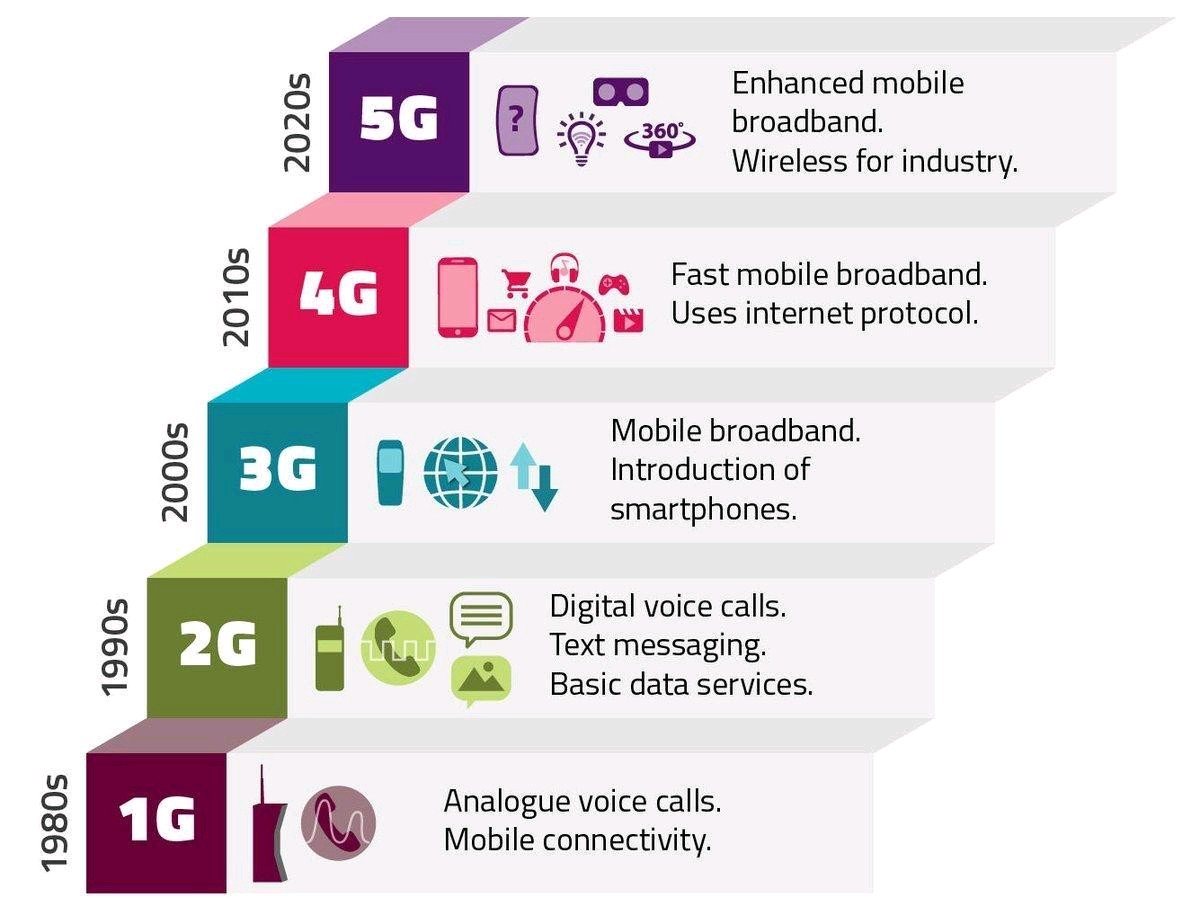
\includegraphics[width=0.75\textwidth]{Images/Chapter1/wireless_evolution.jpg}
    \caption[Evolution of wireless communication systems from 1G to 5G.]{Evolution of wireless communication systems from 1G to 5G~\protect\cite{Fig5GrowthWirelessEvolution}.}
    \label{fig:wireless_evolution}
\end{figure}

\subsubsection{Challenges in High-Mobility Communications}

Future wireless networks are expected to operate in highly dynamic environments, including high-speed trains, unmanned aerial vehicles (UAVs), vehicular communications, and low-earth-orbit satellite systems. In such scenarios, the wireless channel experiences rapid temporal variations caused by the relative motion between transmitters, receivers, and surrounding scatterers. These variations introduce significant Doppler shifts and Doppler spreads, making reliable communication increasingly challenging.

In addition to Doppler effects, multipath propagation generates delay spread due to the presence of multiple reflected signal components arriving at different times. The combined impact of delay spread and Doppler spread results in a doubly selective channel, where the channel varies across both time and frequency domains. Under these conditions, conventional communication systems often suffer from severe performance degradation because the channel characteristics change rapidly within a transmission frame.

As illustrated in Fig.~\ref{fig:ch1_channel_impairments}, multipath propagation introduces delay spread due to the existence of multiple signal propagation paths with different delays. Meanwhile, the relative motion between the transmitter, receiver, and scatterers produces Doppler spread, resulting in frequency shifts that vary among propagation paths.

\begin{figure}[H]
    \centering
    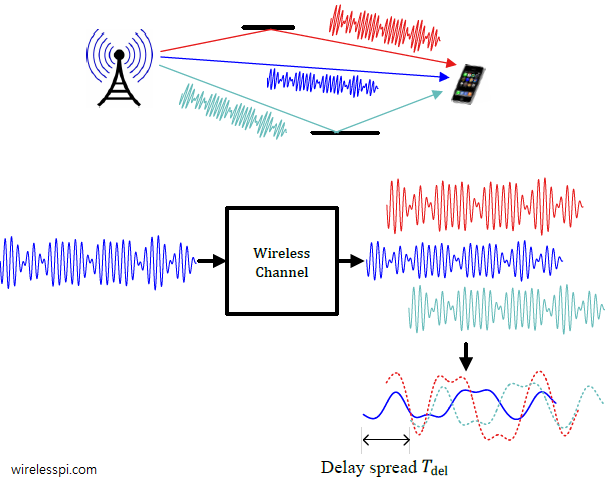
\includegraphics[width=0.8\textwidth]{Images/Chapter1/tre.png}
    \caption[Fundamental channel impairments in high-mobility wireless communications.]{Fundamental channel impairments in high-mobility wireless communications~\protect\cite{WirelessPiSmallScaleFading}.}
    \label{fig:ch1_channel_impairments}
\end{figure}

\subsubsection{Limitations of OFDM Systems}

Orthogonal Frequency Division Multiplexing (OFDM) has become the dominant modulation technique in modern wireless standards due to its ability to efficiently combat frequency-selective fading. By dividing the available bandwidth into multiple orthogonal subcarriers, OFDM converts a frequency-selective channel into a set of parallel flat-fading subchannels, allowing low-complexity one-tap equalization at the receiver.

However, the effectiveness of OFDM relies on the assumption that the wireless channel remains approximately constant during one OFDM symbol interval. In high-mobility environments, significant Doppler shifts destroy the orthogonality among subcarriers and introduce inter-carrier interference (ICI). As a result, the channel matrix loses its desirable diagonal structure, making equalization more difficult and reducing system reliability. Furthermore, the overall performance of an OFDM system is often constrained by the weakest subcarrier, leading to reduced robustness under rapidly time-varying channel conditions.

These limitations motivate the investigation of alternative waveform designs capable of operating effectively in doubly selective channels. Orthogonal Time Frequency Space (OTFS) modulation has recently emerged as a promising candidate, as it represents wireless channels in the delay-Doppler domain and provides improved resilience against high Doppler effects compared with conventional OFDM systems~\cite{Hadani2017OTFSWCNC,Hadani2018OTFS,Wei2020OTFSPromising}.

\begin{figure}[H]
    \centering
    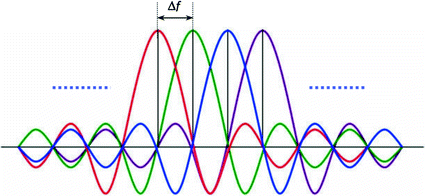
\includegraphics[width=0.75\textwidth]{Images/Chapter1/ici.png}
    \caption[Loss of subcarrier orthogonality and inter-carrier interference in OFDM under high Doppler conditions.]{Loss of subcarrier orthogonality and inter-carrier interference in OFDM under high Doppler conditions~\protect\cite{ScienceDirectICI}.}
    \label{fig:ch1_ofdm_ici}
\end{figure}

\subsubsection{Practical Application Context and Research Problem}

The practical motivation of this thesis comes from wireless links in which mobility and multipath propagation occur simultaneously. Examples include high-speed railway communications, vehicle-to-everything links, unmanned aerial vehicle communication, and satellite-assisted mobile access. In these scenarios, the received signal may contain multiple delayed replicas of the transmitted waveform, while the relative motion of terminals and scatterers introduces Doppler shifts. The resulting channel is difficult to handle with conventional time-frequency-domain designs because the channel response may vary significantly within a transmission frame.

The central physical-layer problem addressed in this thesis is therefore not only how to improve BER performance under a Doppler-affected channel, but also how to evaluate the trade-off between reliability and spectral efficiency when index-based transmission is introduced into OTFS. Baseline OTFS provides a delay-Doppler-domain modulation framework that is suitable for doubly selective channels, whereas OTFS-IM introduces additional information through the activation pattern of delay-Doppler resource elements. However, this additional flexibility also creates a design question: the selected activation patterns, the number of active positions, and the receiver detector jointly affect the final error performance.

For this reason, the thesis studies OTFS-IM as a high-mobility-inspired transmission scheme over discrete delay-Doppler channels. The goal is to evaluate how OTFS-IM behaves compared with baseline OTFS and OFDM-LMMSE references, and to examine whether distance-aware activation pattern selection can improve the reliability of index detection. This framing keeps the study close to practical high-mobility applications while remaining consistent with the MATLAB simulation model developed in the later chapters.

\subsection{Overview of OTFS and Index Modulation}

\subsubsection{Orthogonal Time Frequency Space Modulation}

Orthogonal Time Frequency Space (OTFS) modulation has recently emerged as a promising waveform candidate for future wireless communication systems operating in highly dynamic environments. Unlike conventional OFDM, which multiplexes information symbols in the time-frequency domain, OTFS maps information symbols onto the delay-Doppler domain before transmission~\cite{Hadani2017OTFSWCNC,Hong2019OTFSTutorial}. This alternative signal representation allows the wireless channel to be characterized by a small number of relatively stable propagation paths, each associated with a specific delay and Doppler shift.

The fundamental idea behind OTFS is to transform a rapidly time-varying wireless channel into a nearly invariant representation in the delay-Doppler domain. As a result, all transmitted symbols experience approximately the same channel conditions and can exploit the full time-frequency diversity available in the channel. This characteristic makes OTFS particularly attractive for high-mobility communication scenarios where conventional OFDM systems suffer from severe performance degradation.

Compared with OFDM, OTFS has demonstrated superior robustness against Doppler effects and improved reliability in doubly selective channels. Consequently, OTFS has attracted significant research interest and is considered a potential waveform candidate for beyond-5G and future 6G wireless communication systems.

\begin{figure}[H]
    \centering
    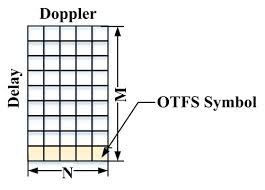
\includegraphics[width=0.88\textwidth]{Images/Chapter1/otfsframe.jpeg}
    \caption[Conceptual framework of OTFS modulation in the delay-Doppler domain.]{Conceptual framework of OTFS modulation in the delay-Doppler domain~\protect\cite{ACM3711129}.}
    \label{fig:otfs_framework}
\end{figure}

\subsubsection{Index Modulation Techniques}

Index Modulation (IM) is a transmission technique that conveys information not only through conventional modulation symbols but also through the indices of selected communication resources~\cite{Basar2016IndexMod5G,Cheng2017IndexMod5G,DoganTusha2020MultidimIM}. Depending on the system configuration, these resources may correspond to subcarriers, antennas, time slots, or other transmission entities. By exploiting additional degrees of freedom for information transmission, IM can improve spectral efficiency without requiring a proportional increase in bandwidth or transmission power.

One of the most widely studied forms of IM is Orthogonal Frequency Division Multiplexing with Index Modulation (OFDM-IM), where only a subset of subcarriers is activated during each transmission interval. The indices of the active subcarriers carry additional information bits, while the active subcarriers simultaneously transmit conventional modulation symbols. Similar concepts have also been extended to multiple-input multiple-output (MIMO) systems and various multicarrier communication frameworks.

The primary advantages of IM include improved spectral efficiency, enhanced flexibility in resource allocation, and the possibility of achieving favorable performance-complexity trade-offs. These characteristics make IM an attractive candidate for integration with advanced waveform technologies in next-generation wireless communication systems.

\begin{figure}[H]
\centering

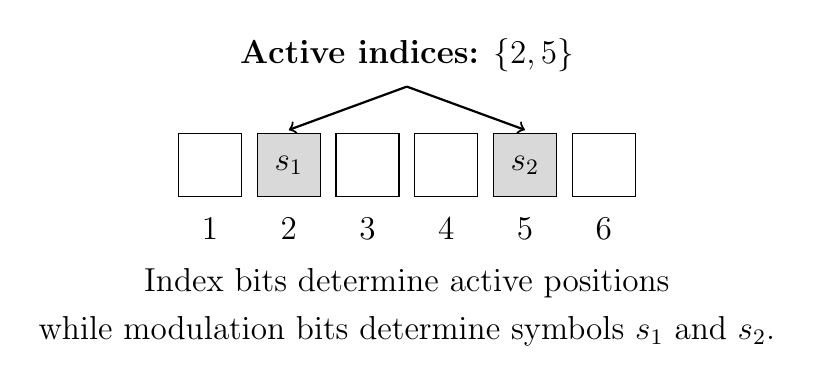
\begin{tikzpicture}[
    every node/.style={font=\small},
    active/.style={draw, fill=gray!30, minimum width=0.8cm, minimum height=0.8cm},
    inactive/.style={draw, minimum width=0.8cm, minimum height=0.8cm}
]

% Resource elements
\node[inactive] (a1) at (0,0) {};
\node[active]   (a2) at (1,0) {$s_1$};
\node[inactive] (a3) at (2,0) {};
\node[inactive] (a4) at (3,0) {};
\node[active]   (a5) at (4,0) {$s_2$};
\node[inactive] (a6) at (5,0) {};

% Index labels
\node at (0,-0.8) {1};
\node at (1,-0.8) {2};
\node at (2,-0.8) {3};
\node at (3,-0.8) {4};
\node at (4,-0.8) {5};
\node at (5,-0.8) {6};

% Text
\node[align=center] at (2.5,1.4)
{\textbf{Active indices:} $\{2,5\}$};

\node[align=center] at (2.5,-1.8)
{Index bits determine active positions\\
while modulation bits determine symbols $s_1$ and $s_2$.};

\draw[->, thick] (2.5,1.0) -- (1,0.45);
\draw[->, thick] (2.5,1.0) -- (4,0.45);

\end{tikzpicture}

\caption{Illustration of information transmission using active index patterns.}
\label{fig:index_modulation}

\end{figure}

\subsubsection{OTFS with Index Modulation}

The integration of Index Modulation into the OTFS framework leads to a new transmission scheme known as OTFS with Index Modulation (OTFS-IM). In this approach, information bits are divided into two groups. One group determines the activation pattern of delay-Doppler resource elements, while the remaining bits are mapped onto conventional constellation symbols transmitted through the activated resources.

By jointly exploiting symbol modulation and index-based information transmission, OTFS-IM can provide additional design flexibility and may improve spectral efficiency depending on the selected activation configuration. The resulting system benefits from both the delay-Doppler diversity offered by OTFS and the additional information-carrying capability introduced by IM.

Recent studies have demonstrated that OTFS-IM can achieve competitive error-rate performance while providing enhanced transmission efficiency under doubly selective fading channels. These promising characteristics motivate further investigation into the design, implementation, and performance evaluation of OTFS-IM systems, which forms the primary focus of this thesis.

\begin{figure}[H]
\centering

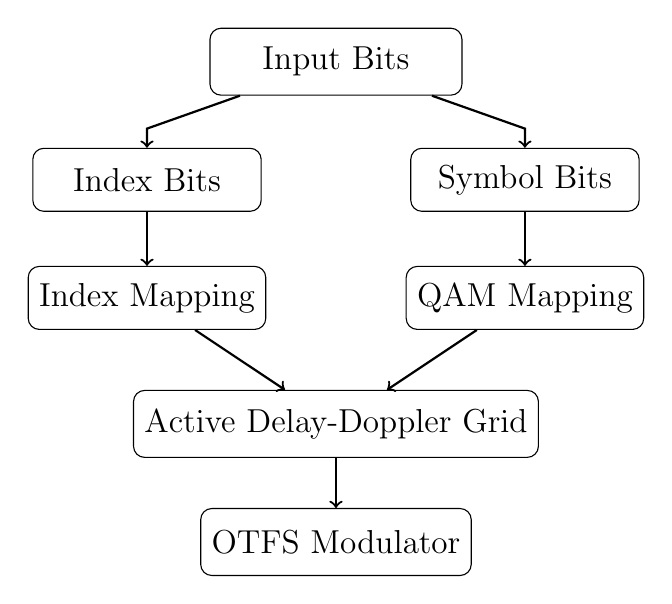
\begin{tikzpicture}[
    node distance=1.15cm,
    every node/.style={font=\small},
    block/.style={
        draw,
        rounded corners,
        minimum width=3.2cm,
        minimum height=0.85cm,
        align=center
    },
    smallblock/.style={
        draw,
        rounded corners,
        minimum width=2.9cm,
        minimum height=0.8cm,
        align=center
    },
    arrow/.style={->, thick}
]

% Main input
\node[block] (bits) at (0,0) {Input Bits};

% Split branches
\node[smallblock] (indexbits) at (-2.4,-1.5) {Index Bits};
\node[smallblock] (symbolbits) at (2.4,-1.5) {Symbol Bits};

\node[smallblock] (indexmap) at (-2.4,-3.0) {Index Mapping};
\node[smallblock] (qammap) at (2.4,-3.0) {QAM Mapping};

% Merge
\node[block] (ddgrid) at (0,-4.6) {Active Delay-Doppler Grid};

\node[block] (otfs) at (0,-6.1) {OTFS Modulator};

% Arrows
\draw[arrow] (bits) -- (-2.4,-0.85) -- (indexbits);
\draw[arrow] (bits) -- (2.4,-0.85) -- (symbolbits);

\draw[arrow] (indexbits) -- (indexmap);
\draw[arrow] (symbolbits) -- (qammap);

\draw[arrow] (indexmap) -- (ddgrid);
\draw[arrow] (qammap) -- (ddgrid);

\draw[arrow] (ddgrid) -- (otfs);

\end{tikzpicture}

\caption{Basic principle of information transmission in an OTFS-IM system.}
\label{fig:otfs_im_concept}

\end{figure}

\subsection{Related Works}

Research on high-mobility wireless transmission has shown that conventional OFDM can suffer from severe inter-carrier interference when Doppler effects are strong~\cite{Hadani2017OTFSWCNC,Wei2020OTFSPromising,Raviteja2018OTFSInterference}. Although OFDM remains attractive because of its simple FFT-based implementation and low-complexity equalization, its performance depends heavily on the preservation of subcarrier orthogonality. This limitation has motivated the study of alternative modulation schemes that are more suitable for doubly selective channels.

OTFS was introduced as a delay-Doppler-domain modulation technique to improve robustness in time-varying channels~\cite{Hadani2017OTFSWCNC,Hadani2018OTFS,Wei2020OTFSPromising,Hong2019OTFSTutorial}. Later works further analyzed OTFS input-output relations, interference behavior, and receiver design, including message passing and linear equalization methods~\cite{Raviteja2018OTFSMP,Raviteja2018OTFSInterference,Surabhi2020LinearEqualization}. These studies indicate that representing the channel in the delay-Doppler domain can provide a more stable structure for high-mobility communication than conventional time-frequency-domain processing.

In parallel, Index Modulation has been widely studied as a method for transmitting extra information through the indices of active resources~\cite{Basar2016IndexMod5G,Cheng2017IndexMod5G,DoganTusha2020MultidimIM}. OFDM-IM is a representative example, where only a subset of subcarriers is activated and the active-subcarrier pattern carries additional bits~\cite{Wen2017OFDMIM}. This principle can improve flexibility in the trade-off among reliability, spectral efficiency, and detection complexity.

Recent studies have extended the IM concept to OTFS systems and reported that OTFS-IM can achieve promising BER and spectral-efficiency performance over doubly selective channels~\cite{Liang2020OTFSIM,Qian2022BlockWiseOTFSIM,Qian2023ReceiverOTFSIM,Wu2024OTFSIMDetector}. However, the final performance of OTFS-IM depends strongly on activation-pattern design, the number of active delay-Doppler positions, and the receiver detection method. Therefore, this thesis focuses on a simulation-based evaluation of OTFS-IM, with particular attention to distance-aware activation-pattern selection and the decomposition of total BER into index and symbol error components. This provides the basis for the research objectives and methodology presented in the following section.

\subsection{Research Objectives and Methodology}

\subsubsection{Research Objectives}

The primary objective of this thesis is to investigate the applicability of Orthogonal Time Frequency Space modulation combined with Index Modulation techniques for high-mobility-inspired wireless communication environments. The study focuses on analyzing the performance characteristics of OTFS-IM systems and evaluating their potential advantages and limitations compared with conventional OTFS transmission schemes.

To achieve this objective, the theoretical foundations of OTFS modulation and Index Modulation are first studied in detail. Particular attention is given to the representation of wireless channels in the delay-Doppler domain, which forms the basis for the robustness of OTFS under rapidly time-varying channel conditions. Furthermore, the principles of index-based information transmission are investigated to understand how additional information can be conveyed through the activation patterns of transmission resources.

Based on these theoretical foundations, an OTFS-IM transmission framework is developed and implemented in MATLAB. The proposed system is evaluated under doubly selective fading channels with various signal-to-noise ratios. The performance of the system is assessed primarily in terms of Bit Error Rate (BER), while the impact of different index activation patterns, modulation parameters, and spectral-efficiency configurations is also examined.

The final objective of the thesis is to provide a comprehensive performance evaluation of OTFS-IM and to identify its potential benefits and limitations for future high-mobility wireless communication systems. The obtained results are expected to contribute to the ongoing development of waveform technologies for beyond-5G and sixth-generation (6G) communication networks.

\subsubsection{Main Contributions of the Thesis}

The first contribution of this thesis is the development of a MATLAB-based simulation framework for comparing OFDM-LMMSE, baseline OTFS, and OTFS-IM under a common delay-Doppler channel model. This framework allows the effect of Doppler-aware signal representation and index-based transmission to be evaluated within the same physical-layer setting.

The second contribution is the construction and evaluation of an OTFS-IM transmission chain in which information bits are divided into index bits and constellation bits. Different activation configurations are considered in order to study how the number of active positions affects BER performance and spectral efficiency. This is important because OTFS-IM does not always improve all performance metrics simultaneously; instead, it introduces a reliability-efficiency trade-off that must be analyzed carefully.

The third contribution is the investigation of activation-pattern selection strategies for OTFS-IM. In particular, Hamming-distance-aware pattern selection and its balanced variant are examined as rule-based methods for selecting delay-Doppler activation patterns. These methods are compared with random pattern selection to assess whether larger pairwise pattern separation and more balanced carrier usage can improve index detection reliability.

The final contribution is a multi-level performance analysis that includes total BER, index BER, symbol BER, pattern error rate, and BER-spectral-efficiency trade-off across several OTFS-IM configurations. Instead of relying on a single BER curve, the thesis analyzes where the performance gain or loss originates, thereby providing a clearer interpretation of the behavior of OTFS-IM systems under the considered simulation assumptions.

\subsubsection{Research Scope}

This thesis focuses on the investigation of OTFS modulation and OTFS with Index Modulation under high-mobility-inspired wireless communication scenarios. The study is limited to single-user transmission systems and considers doubly selective fading channels characterized by both delay spread and Doppler spread.

The research primarily concentrates on the physical layer aspects of wireless communication systems. Channel coding, medium access control protocols, resource scheduling, and higher-layer networking issues are beyond the scope of this work. Instead, emphasis is placed on signal modulation, index mapping strategies, delay-Doppler domain processing, and receiver detection techniques.

A simulation-based approach is adopted throughout the study. The performance evaluation is carried out using MATLAB-based implementations of both conventional OTFS and OTFS-IM systems. The considered performance metric is the Bit Error Rate (BER), which is evaluated under different signal-to-noise ratio conditions. Various system parameters, including modulation order and index activation configurations, are investigated to analyze their influence on system performance.

It should be noted that practical implementation issues such as hardware impairments, synchronization errors, channel estimation inaccuracies, and real-time processing constraints are not explicitly addressed in this thesis. These aspects are left for future research and experimental validation.

\subsubsection{Research Methodology}

The research methodology adopted in this thesis consists of four main stages, including theoretical analysis, system modeling, simulation implementation, and performance evaluation.

The first stage involves an extensive review of the existing literature related to wireless communication systems operating in high-mobility environments. Particular attention is given to the theoretical principles of OTFS modulation, delay-Doppler domain channel representation, and Index Modulation techniques. Relevant research articles, tutorial papers, and recent survey studies are examined to establish a comprehensive theoretical foundation for the proposed work.

The second stage focuses on the development of mathematical models for both OTFS and OTFS-IM systems. The signal processing procedures involved in transmission and reception are analyzed, including symbol mapping, index selection, delay-Doppler domain modulation, channel propagation, and receiver detection. These models provide the basis for the simulation framework employed throughout the study.

The third stage consists of implementing the developed models in MATLAB. The simulation environment is designed to emulate high-mobility wireless channels with varying Doppler conditions and additive white Gaussian noise. Different system configurations are considered to investigate the influence of modulation parameters and index activation strategies on communication performance.

The final stage involves analyzing and comparing the obtained simulation results. The BER performance of conventional OTFS and OTFS-IM systems is evaluated over a range of signal-to-noise ratios. Based on the observed results, conclusions are drawn regarding the effectiveness of index modulation in improving the performance and transmission efficiency of OTFS systems under challenging wireless channel conditions.

\begin{figure}[H]
    \centering
    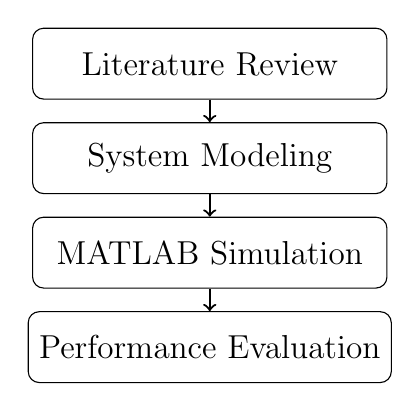
\begin{tikzpicture}[
        node distance=1.2cm,
        block/.style={
            draw,
            rounded corners,
            minimum width=4.5cm,
            minimum height=0.9cm,
            align=center
        },
        arrow/.style={->, thick}
    ]

    \node[block] (lit) {Literature Review};

    \node[block, below of=lit] (model) {System Modeling};

    \node[block, below of=model] (sim) {MATLAB Simulation};

    \node[block, below of=sim] (eval) {Performance Evaluation};

    \draw[arrow] (lit) -- (model);
    \draw[arrow] (model) -- (sim);
    \draw[arrow] (sim) -- (eval);

    \end{tikzpicture}

    \caption{Research methodology adopted in this thesis.}
    \label{fig:research_methodology}
\end{figure}

\subsection{Thesis Organization}

The remainder of this thesis is organized as follows.

Chapter 2 presents the theoretical background required for understanding the proposed system. Fundamental concepts of wireless communication channels, multipath propagation, Doppler effects, Orthogonal Frequency Division Multiplexing (OFDM), delay-Doppler domain representation, and Index Modulation techniques are reviewed. The limitations of conventional multicarrier systems in high-mobility environments are also discussed.

Chapter 3 introduces the principles of Orthogonal Time Frequency Space (OTFS) modulation. The OTFS transmitter and receiver structures, delay-Doppler domain signal representation, modulation and demodulation processes, and input-output relationships are presented. The advantages of OTFS over conventional OFDM systems in doubly selective channels are also analyzed.

Chapter 4 focuses on the integration of Index Modulation into the OTFS framework. The operating principles of OTFS-IM, index mapping strategies, resource activation patterns, transmitter and receiver architectures, and detection mechanisms are described. Furthermore, the expected benefits and design considerations of OTFS-IM systems are discussed.

Chapter 5 presents the simulation framework and performance evaluation of the proposed systems. MATLAB-based implementations of OTFS and OTFS-IM are developed and tested under various channel conditions. The performance of the considered schemes is evaluated primarily in terms of Bit Error Rate (BER), and comparisons are conducted to investigate the impact of different system parameters and index activation configurations.

Finally, Chapter 6 summarizes the main findings of the thesis and highlights the key contributions of the conducted research. Possible directions for future work and further improvements of OTFS-IM systems are also suggested.

\begin{figure}[H]
    \centering
    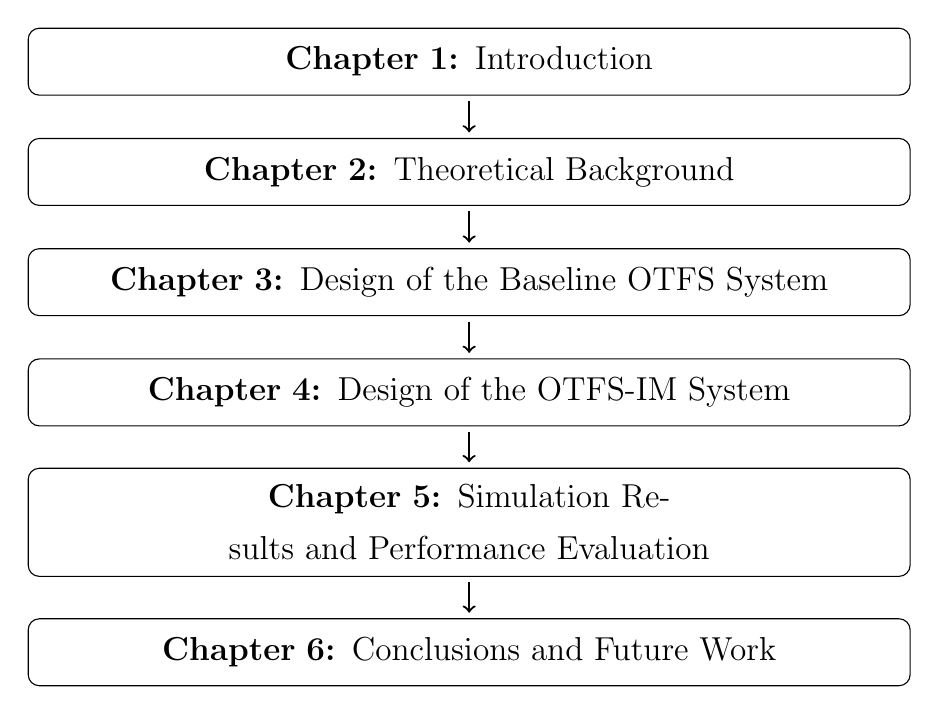
\begin{tikzpicture}[
        block/.style={
            draw,
            rounded corners,
            minimum width=11.2cm,
            minimum height=0.85cm,
            text width=10.4cm,
            align=center,
            inner sep=6pt
        },
        arrow/.style={->, thick, shorten >=2pt, shorten <=2pt}
    ]

    \node[block] (c1) at (0,0) {\textbf{Chapter 1:} Introduction};
    \node[block] (c2) at (0,-1.40) {\textbf{Chapter 2:} Theoretical Background};
    \node[block] (c3) at (0,-2.80) {\textbf{Chapter 3:} Design of the Baseline OTFS System};
    \node[block] (c4) at (0,-4.20) {\textbf{Chapter 4:} Design of the OTFS-IM System};
    \node[block] (c5) at (0,-5.85) {\textbf{Chapter 5:} Simulation Results and Performance Evaluation};
    \node[block] (c6) at (0,-7.50) {\textbf{Chapter 6:} Conclusions and Future Work};

    \draw[arrow] (c1) -- (c2);
    \draw[arrow] (c2) -- (c3);
    \draw[arrow] (c3) -- (c4);
    \draw[arrow] (c4) -- (c5);
    \draw[arrow] (c5) -- (c6);

    \end{tikzpicture}

    \caption{Thesis structure and chapter progression.}
    \label{fig:thesis_organization}
\end{figure}

The structure presented in Fig.~\ref{fig:thesis_organization} illustrates the logical flow of the research conducted in this thesis. The organization begins with the research motivation and theoretical background, followed by the baseline OTFS system design and the OTFS-IM extension. The developed systems are then evaluated through simulation, and the final chapter summarizes the main findings, limitations, and future research directions.

\newpage

\section*{CHAPTER 2. THEORETICAL BACKGROUND}
\addcontentsline{toc}{section}{CHAPTER 2. THEORETICAL BACKGROUND}

% =========================================================
% Numbering for Chapter 2
% =========================================================
\setcounter{section}{2}
\setcounter{subsection}{0}
\setcounter{subsubsection}{0}
\setcounter{figure}{0}
\setcounter{table}{0}
\setcounter{equation}{0}

\renewcommand{\thefigure}{2.\arabic{figure}}
\renewcommand{\thetable}{2.\arabic{table}}
\renewcommand{\theequation}{2.\arabic{equation}}
\renewcommand{\theHfigure}{2.\arabic{figure}}
\renewcommand{\theHtable}{2.\arabic{table}}
\renewcommand{\theHequation}{2.\arabic{equation}}

% =========================================================
% Chapter Introduction
% =========================================================
This chapter presents the theoretical foundations required for the study of OTFS and OTFS-IM systems. Fundamental concepts related to wireless communication channels, multipath propagation, Doppler effects, OFDM transmission, delay-Doppler signal representation, and index modulation techniques are reviewed~\cite{Hong2019OTFSTutorial,Basar2016IndexMod5G,Wen2017OFDMIM}. These concepts provide the necessary background for the development and analysis of the proposed systems in the subsequent chapters.


% =========================================================
% Chapter Sections
% =========================================================
\subsection{Wireless Communication Channels}

Wireless communication channels provide the medium through which information is transmitted between communicating devices. Due to the random nature of the propagation environment, wireless signals are affected by various phenomena that influence transmission quality and system performance. Therefore, understanding the characteristics, impairments, and classification of wireless channels is essential for the design and analysis of modern communication systems.

\subsubsection{Wireless Channel Characteristics}

A wireless communication channel represents the physical medium through which electromagnetic waves propagate from a transmitter to a receiver. Unlike wired channels, where the transmission medium is fixed and relatively predictable, wireless channels are inherently dynamic and strongly influenced by the surrounding environment. Buildings, vehicles, terrain, and moving objects may alter the propagation path of transmitted signals, resulting in significant variations in the received waveform.

In communication theory, a wireless channel is commonly modeled as a linear system that modifies the transmitted signal during propagation. The received signal can generally be expressed as

\begin{equation}
y(t)=h(t)\ast x(t)+n(t)
\end{equation}

where $x(t)$ is the transmitted signal, $y(t)$ is the received signal, $h(t)$ denotes the channel impulse response, $\ast$ represents the convolution operation, and $n(t)$ denotes additive noise.

The channel impulse response contains information regarding the propagation environment and determines how the transmitted signal is transformed before reaching the receiver. Variations in the channel response arise from factors such as propagation distance, obstacles, mobility, and environmental conditions.

\begin{figure}[H]
    \centering

    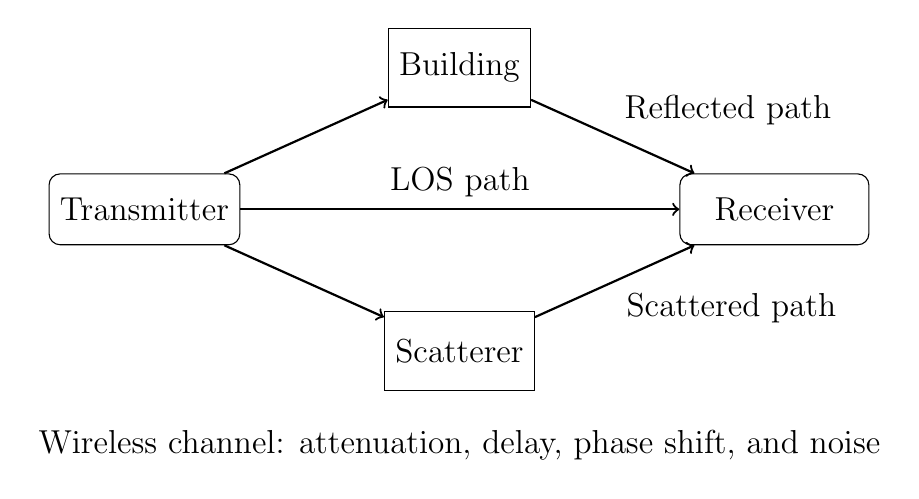
\begin{tikzpicture}[
        every node/.style={font=\small},
        block/.style={
            draw,
            rounded corners,
            minimum width=2.4cm,
            minimum height=0.9cm,
            align=center
        },
        obj/.style={
            draw,
            minimum width=1.2cm,
            minimum height=1.0cm,
            align=center
        },
        arrow/.style={->, thick}
    ]

    % Transmitter and receiver
    \node[block] (tx) at (0,0) {Transmitter};
    \node[block] (rx) at (8,0) {Receiver};

    % Objects
    \node[obj] (building) at (4,1.8) {Building};
    \node[obj] (scatterer) at (4,-1.8) {Scatterer};

    % Direct path
    \draw[arrow] (tx) -- node[above] {LOS path} (rx);

    % Reflected path
    \draw[arrow] (tx) -- (building);
    \draw[arrow] (building) -- node[above right] {Reflected path} (rx);

    % Scattered path
    \draw[arrow] (tx) -- (scatterer);
    \draw[arrow] (scatterer) -- node[below right] {Scattered path} (rx);

    % Channel label
    \node[align=center] at (4,-3.0)
    {Wireless channel: attenuation, delay, phase shift, and noise};

    \end{tikzpicture}

    \caption{General representation of a wireless communication channel.}
    \label{fig:wireless_channel_model}
\end{figure}

Figure~\ref{fig:wireless_channel_model} illustrates a typical wireless propagation scenario. Instead of following a single direct path, the transmitted signal may arrive at the receiver through multiple propagation paths generated by reflection, diffraction, and scattering mechanisms.

The unique characteristics of wireless channels distinguish them from wired transmission media. Signal attenuation increases with propagation distance, multiple signal replicas may be received due to multipath propagation, and mobility introduces time-varying channel behavior. These characteristics collectively create significant challenges for reliable wireless communication.

\subsubsection{Channel Impairments}

During propagation, wireless signals are subjected to various impairments that degrade transmission quality and limit communication performance. These impairments originate from the physical characteristics of the propagation environment as well as from practical limitations of communication hardware. Understanding their effects is essential for the design of reliable wireless transmission systems.

One of the most fundamental impairments is path loss, which refers to the gradual reduction in signal power as the propagation distance increases. In practical environments, obstacles such as buildings, vegetation, and terrain irregularities introduce additional attenuation, commonly known as shadowing. These effects reduce the received signal strength and may significantly limit communication coverage.

Another important impairment is multipath fading. Due to reflections, diffraction, and scattering, multiple copies of the transmitted signal arrive at the receiver through different propagation paths. Since these signal components experience different delays and phases, constructive and destructive interference may occur, leading to fluctuations in the received signal amplitude and phase.

Wireless communication systems are also affected by Doppler effects caused by relative motion between the transmitter, receiver, or surrounding scatterers. Doppler shifts introduce frequency offsets and time variations into the channel response, which become increasingly significant in high-mobility scenarios such as vehicular communications, high-speed railways, and unmanned aerial vehicle networks.

In addition, all practical receivers are affected by thermal noise generated by electronic components. This disturbance is commonly modeled as Additive White Gaussian Noise (AWGN) and represents a fundamental source of performance degradation in wireless communication systems.

\begin{figure}[H]
    \centering

    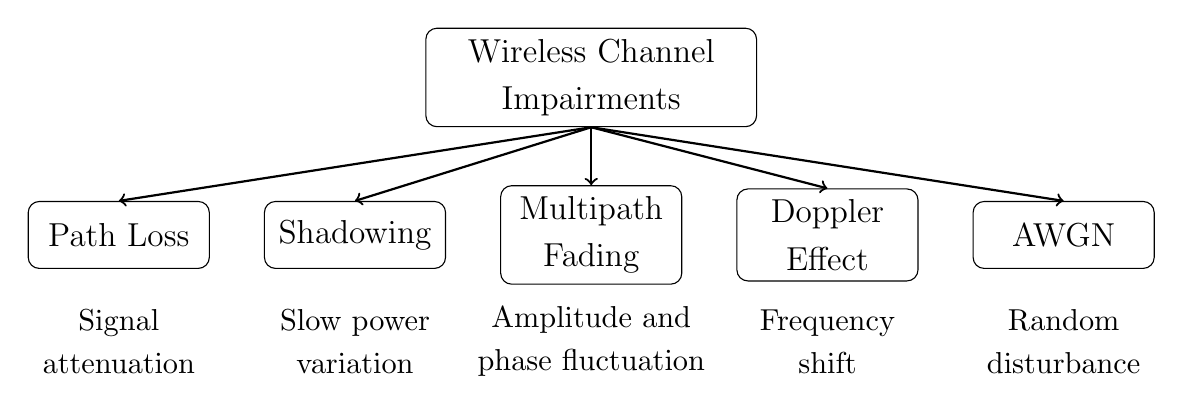
\begin{tikzpicture}[
        every node/.style={font=\small},
        main/.style={
            draw,
            rounded corners,
            minimum width=4.2cm,
            minimum height=1.0cm,
            align=center
        },
        item/.style={
            draw,
            rounded corners,
            minimum width=2.3cm,
            minimum height=0.85cm,
            align=center
        },
        desc/.style={
            align=center,
            font=\footnotesize
        },
        arrow/.style={->, thick}
    ]

    % Main node
    \node[main] (channel) at (0,0) {Wireless Channel\\Impairments};

    % Impairment nodes - increased spacing
    \node[item] (pathloss)  at (-6.0,-2.0) {Path Loss};
    \node[item] (shadowing) at (-3.0,-2.0) {Shadowing};
    \node[item] (multipath) at (0,-2.0) {Multipath\\Fading};
    \node[item] (doppler)   at (3.0,-2.0) {Doppler\\Effect};
    \node[item] (noise)     at (6.0,-2.0) {AWGN};

    % Arrows
    \draw[arrow] (channel.south) -- (pathloss.north);
    \draw[arrow] (channel.south) -- (shadowing.north);
    \draw[arrow] (channel.south) -- (multipath.north);
    \draw[arrow] (channel.south) -- (doppler.north);
    \draw[arrow] (channel.south) -- (noise.north);

    % Descriptions
    \node[desc] at (-6.0,-3.35) {Signal\\attenuation};
    \node[desc] at (-3.0,-3.35) {Slow power\\variation};
    \node[desc] at (0,-3.35) {Amplitude and\\phase fluctuation};
    \node[desc] at (3.0,-3.35) {Frequency\\shift};
    \node[desc] at (6.0,-3.35) {Random\\disturbance};

    \end{tikzpicture}

    \caption{Major impairments affecting wireless communication channels.}
    \label{fig:channel_impairments}
\end{figure}

The major impairments encountered in wireless communication channels and their corresponding effects are summarized in Table~\ref{tab:channel_impairments}.

\begin{table}[H]
\centering
\caption{Common wireless channel impairments and their effects.}
\label{tab:channel_impairments}

\begin{tabular}{|p{3cm}|p{4cm}|p{6cm}|}
\hline
\textbf{Impairment} &
\textbf{Primary Cause} &
\textbf{Effect on System Performance} \\
\hline

Path Loss &
Propagation distance &
Reduction of received signal power \\
\hline

Shadowing &
Obstacles and terrain &
Slow fluctuations in received signal strength \\
\hline

Multipath Fading &
Multiple propagation paths &
Amplitude and phase variations, signal distortion \\
\hline

Doppler Effect &
Relative motion &
Frequency shifts and channel time variations \\
\hline

AWGN &
Thermal noise &
Detection errors and performance degradation \\
\hline

\end{tabular}

\end{table}

The combined effects of path loss, fading, Doppler shifts, and noise represent the primary challenges faced by modern wireless communication systems. These impairments directly influence the design of modulation schemes, channel estimation algorithms, equalization techniques, and receiver architectures. Consequently, accurate channel modeling is a crucial step in the development and evaluation of advanced communication technologies.


\subsubsection{Channel Classification}

Wireless communication channels can be classified according to different characteristics of the propagation environment. Such classifications provide useful insight into channel behavior and help communication engineers select appropriate transmission and receiver techniques for specific operating conditions.

Based on frequency selectivity, wireless channels are generally categorized as flat-fading channels or frequency-selective channels. In a flat-fading channel, all frequency components of the transmitted signal experience approximately the same channel gain and phase shift. Conversely, a frequency-selective channel affects different frequency components differently, resulting in signal distortion and potential inter-symbol interference.

From a temporal perspective, channels may be classified as time-invariant or time-varying. A time-invariant channel remains relatively stable during the transmission interval, whereas a time-varying channel exhibits continuous fluctuations due to user mobility and changes in the propagation environment.

Wireless channels can also be categorized according to propagation conditions. Line-of-Sight (LOS) channels contain a direct propagation path between the transmitter and receiver, while Non-Line-of-Sight (NLOS) channels rely mainly on reflected, diffracted, and scattered signal components.

Table~\ref{tab:channel_classification} summarizes several common criteria used for wireless channel classification.

\begin{table}[H]
\centering
\caption{Classification of wireless communication channels.}
\label{tab:channel_classification}

\begin{tabular}{|p{4cm}|p{4cm}|p{4cm}|}
\hline
\textbf{Classification Criterion} &
\textbf{Category 1} &
\textbf{Category 2} \\
\hline

Frequency Selectivity &
Flat Fading &
Frequency Selective \\
\hline

Time Variation &
Time Invariant &
Time Varying \\
\hline

Propagation Condition &
LOS &
NLOS \\
\hline

Mobility Scenario &
Low Mobility &
High Mobility \\
\hline

\end{tabular}

\end{table}

\begin{figure}[H]
    \centering

    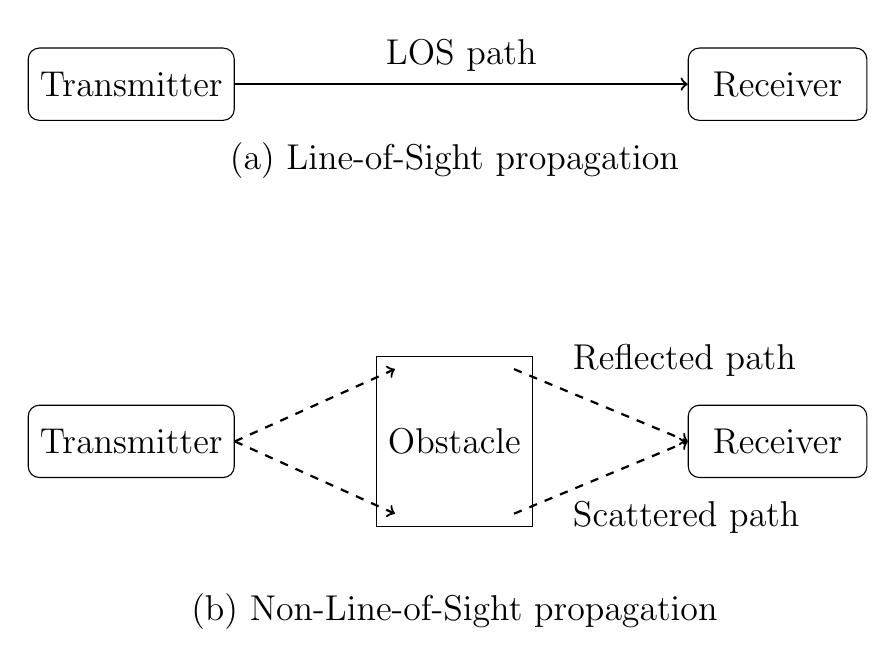
\begin{tikzpicture}[
        scale=1.08,
        transform shape,
        every node/.style={font=\small},
        device/.style={
            draw,
            rounded corners,
            minimum width=2.1cm,
            minimum height=0.85cm,
            align=center
        },
        obstacle/.style={
            draw,
            minimum width=1.45cm,
            minimum height=2.0cm,
            align=center
        },
        arrow/.style={->, thick},
        dashedarrow/.style={->, thick, dashed}
    ]

    % =========================
    % LOS scenario
    % =========================
    \node[device] (tx1) at (0,2.2) {Transmitter};
    \node[device] (rx1) at (7.6,2.2) {Receiver};

    \draw[arrow] (tx1.east) -- node[above] {LOS path} (rx1.west);

    \node[align=center] at (3.8,1.3) {(a) Line-of-Sight propagation};

    % =========================
    % NLOS scenario
    % =========================
    \node[device] (tx2) at (0,-2.0) {Transmitter};
    \node[obstacle] (obs) at (3.8,-2.0) {Obstacle};
    \node[device] (rx2) at (7.6,-2.0) {Receiver};

    % Points near obstacle edges (shorter dashed arrows)
    \coordinate (topL) at (3.1,-1.15);
    \coordinate (topR) at (4.5,-1.15);
    \coordinate (botL) at (3.1,-2.85);
    \coordinate (botR) at (4.5,-2.85);

    % Dashed paths
    \draw[dashedarrow] (tx2.east) -- (topL);
    \draw[dashedarrow] (topR) -- (rx2.west);

    \draw[dashedarrow] (tx2.east) -- (botL);
    \draw[dashedarrow] (botR) -- (rx2.west);

    % Labels moved away from paths
    \node[anchor=west] at (5.05,-1.05) {Reflected path};
    \node[anchor=west] at (5.05,-2.9) {Scattered path};

    \node[align=center] at (3.8,-4.0) {(b) Non-Line-of-Sight propagation};

    \end{tikzpicture}

    \caption{Illustration of LOS and NLOS propagation scenarios.}
    \label{fig:los_nlos}
\end{figure}

Among the various channel categories, high-mobility wireless channels represent one of the most challenging communication environments. In such scenarios, the channel often exhibits both frequency selectivity due to multipath propagation and time selectivity due to Doppler effects. These characteristics lead to the so-called doubly selective channel, which plays a central role in the development of advanced waveform technologies such as OTFS. The propagation mechanisms responsible for these effects are discussed in the following section.


% ~6 pages
\subsection{Multipath Propagation and Doppler Effects}

The performance of wireless communication systems is strongly affected by the physical propagation environment. In practice, wireless signals rarely propagate through a single ideal path. Instead, they are influenced by surrounding objects, user mobility, and the relative motion between transmitters, receivers, and scatterers. Among these effects, multipath propagation and Doppler effects are particularly important because they determine how the wireless channel varies over time and frequency.

In high-mobility scenarios such as vehicular communications, high-speed railways, unmanned aerial vehicles, and low-earth-orbit satellite links, these effects become more severe. Multipath propagation causes the transmitted signal to arrive at the receiver through multiple paths with different delays, while Doppler effects introduce frequency shifts and time variation. These two phenomena provide the basis for understanding doubly selective channels, which are one of the main motivations for advanced waveform designs such as OTFS.

\begin{figure}[H]
    \centering
    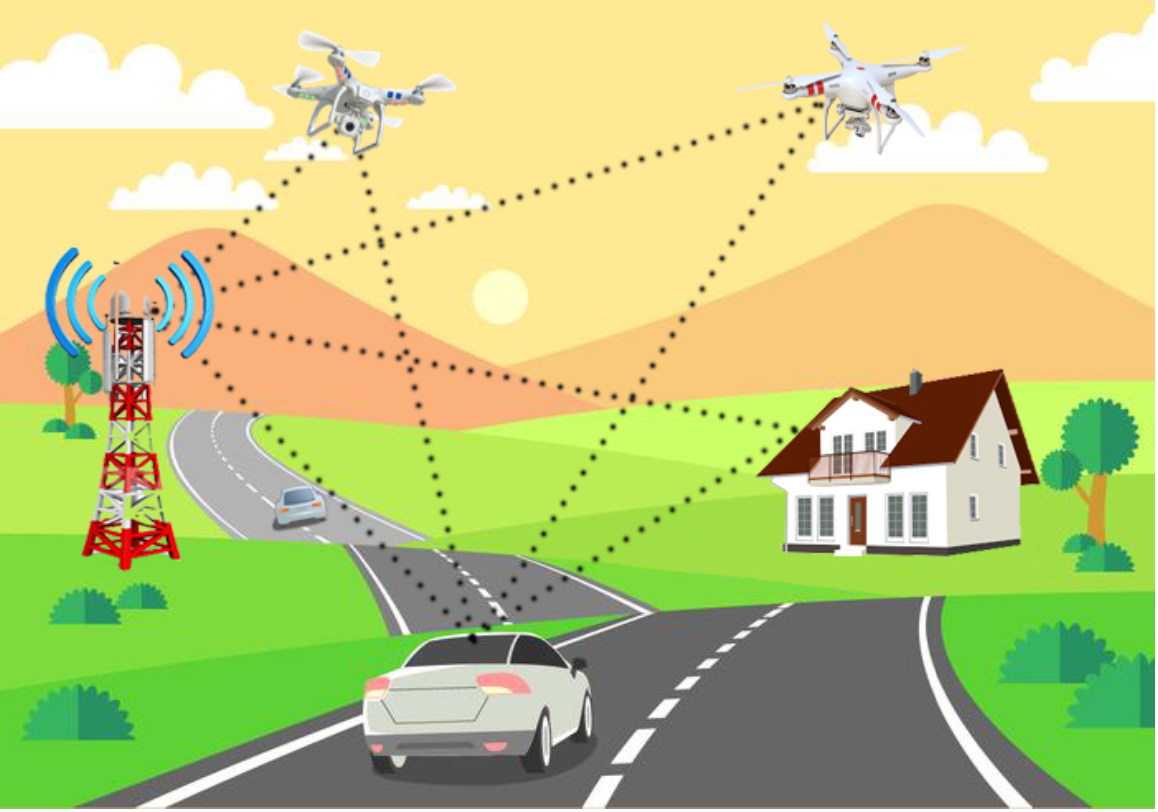
\includegraphics[width=0.82\textwidth]{Images/Chapter2/high_mobility_multipath.png}
    \caption[High-mobility wireless communication scenario with multiple propagation paths.]{High-mobility wireless communication scenario with multiple propagation paths~\protect\cite{Hong2019OTFSTutorial}.}
    \label{fig:high_mobility_multipath}
\end{figure}

Figure~\ref{fig:high_mobility_multipath} illustrates a high-mobility wireless communication scenario in which several terminals and reflecting objects coexist. The transmitted signal may reach the receiver through direct, reflected, diffracted, and scattered paths. Such a propagation environment leads naturally to both delay dispersion and Doppler dispersion.

\subsubsection{Multipath Propagation}

Multipath propagation occurs when transmitted electromagnetic waves reach the receiver through more than one propagation path. These paths may be created by reflection from buildings, diffraction around obstacles, and scattering from irregular objects such as trees, vehicles, and terrain. As a result, the receiver observes several replicas of the transmitted signal rather than a single clean copy.

Each propagation path is generally associated with a different path length. Therefore, the corresponding received signal component has its own delay, amplitude attenuation, and phase shift. The received waveform is formed by the superposition of all these components. Depending on their relative phases, the multipath components may combine constructively or destructively, causing fluctuations in the received signal strength.

A simple multipath channel can be represented as

\begin{equation}
h(t,\tau)=\sum_{i=1}^{P}h_i(t)\delta(\tau-\tau_i),
\end{equation}

where \(P\) is the number of propagation paths, \(h_i(t)\) is the complex channel gain of the \(i\)-th path, and \(\tau_i\) is the propagation delay of that path. This equation only states that the channel is composed of several delayed copies of the transmitted signal.

Figure~\ref{fig:high_mobility_multipath} illustrates the basic idea of multipath propagation. In addition to a possible direct path between the transmitter and receiver, the signal may also arrive through reflected or scattered paths. These additional paths usually travel longer distances and therefore arrive later than the direct component.

Multipath propagation is important because it directly affects the received signal quality. If the delayed components arrive within a short time interval, they may simply cause fading. However, if the delay differences are comparable to the symbol duration, different symbols may overlap at the receiver. This effect is known as inter-symbol interference (ISI).

Although multipath propagation is often considered a source of distortion, it may also provide diversity. Since different propagation paths carry different versions of the transmitted signal, a properly designed receiver can exploit these components to improve reliability. Modern wireless systems use equalization, coding, diversity combining, and multicarrier modulation to reduce the negative effects of multipath and, when possible, benefit from the available path diversity.

In the context of this thesis, multipath propagation is important because it leads to delay spread and frequency selectivity. These concepts are discussed in the next subsection.

\subsubsection{Delay Spread and Frequency Selectivity}

Delay spread is a direct consequence of multipath propagation. Since different propagation paths have different lengths, their corresponding signal components arrive at the receiver at different times. The difference between the earliest and latest significant arriving components is commonly referred to as delay spread.

The propagation delay of a signal path is proportional to the path length and can be expressed as

\begin{equation}
\tau=\frac{d}{c},
\end{equation}

where \(d\) is the propagation distance and \(c\) is the speed of light.

\begin{figure}[H]
    \centering
    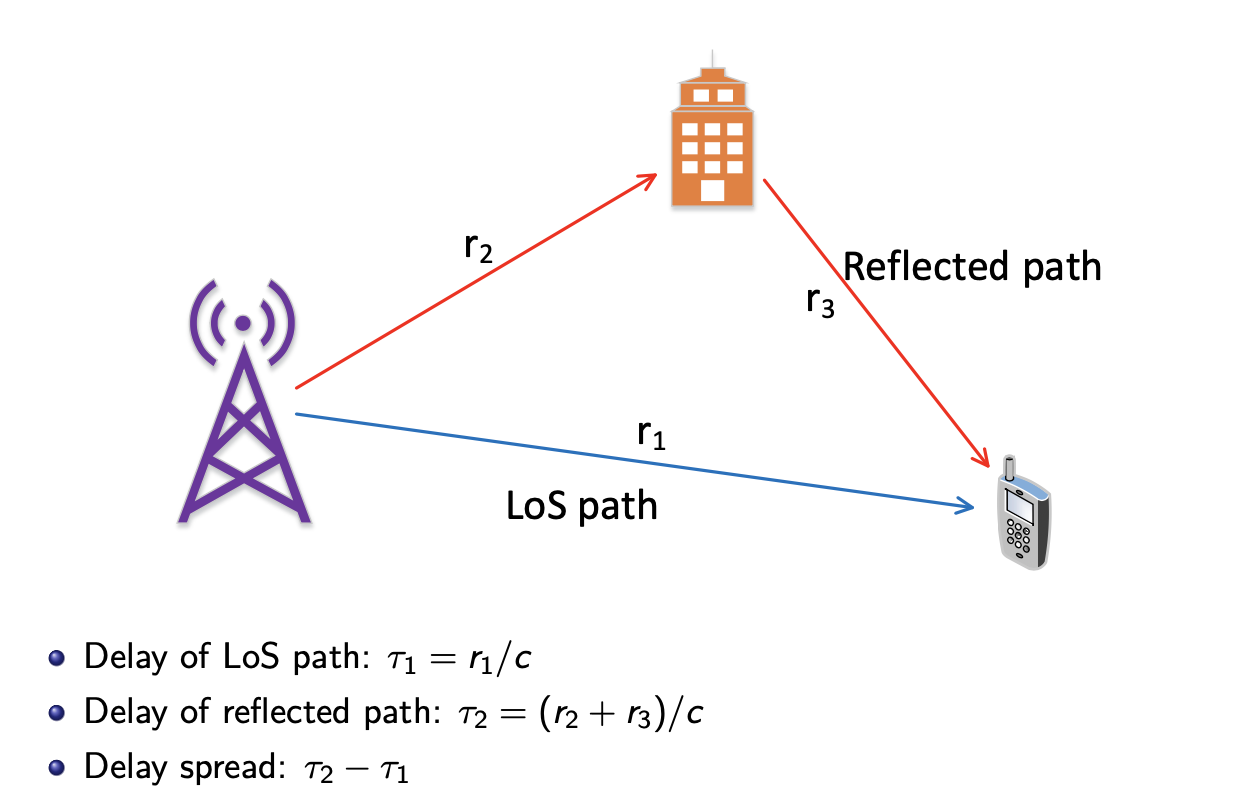
\includegraphics[width=0.82\textwidth]{Images/Chapter2/delay_spread.png}
    \caption[Illustration of delay spread caused by LoS and reflected propagation paths.]{Illustration of delay spread caused by LoS and reflected propagation paths~\protect\cite{Hong2019OTFSTutorial}.}
    \label{fig:delay_spread}
\end{figure}

Figure~\ref{fig:delay_spread} shows a simple example of delay spread. The direct Line-of-Sight (LoS) path travels a distance \(r_1\), while the reflected path travels through two segments with distances \(r_2\) and \(r_3\). Therefore, the corresponding delays can be written as

\begin{equation}
\tau_1=\frac{r_1}{c},
\qquad
\tau_2=\frac{r_2+r_3}{c}.
\end{equation}

The delay spread in this simple case is the difference between these two delays. A larger delay spread means that the received signal components are more spread out in time.

Delay spread has an important effect on the frequency-domain behavior of the channel. When a channel introduces significant delay dispersion, different frequency components of the transmitted signal may experience different attenuation and phase rotation. In this case, the channel is called frequency selective.

If the signal bandwidth is small compared with the frequency range over which the channel response is approximately constant, the channel behaves like a flat-fading channel. In a flat-fading channel, all frequency components of the signal are affected in nearly the same way. Conversely, when the signal bandwidth is large, different frequency components may experience different channel gains. The channel then becomes frequency selective.

Frequency selectivity is a major challenge for broadband communication systems. It can distort the transmitted waveform and create ISI. This is one of the main reasons why OFDM has been widely used in modern wireless systems: OFDM divides a wideband frequency-selective channel into many narrowband subchannels, making equalization much simpler.

Table~\ref{tab:delay_spread_effects} summarizes the relationship between multipath propagation, delay spread, and frequency selectivity.

\begin{table}[H]
\centering
\caption{Effects of multipath propagation and delay spread.}
\label{tab:delay_spread_effects}

\begin{tabular}{|p{4cm}|p{4cm}|p{5cm}|}
\hline
\textbf{Cause} &
\textbf{Channel Effect} &
\textbf{Main Consequence} \\
\hline

Multiple propagation paths &
Different arrival times &
Delay spread \\
\hline

Large delay spread &
Different response across frequency &
Frequency-selective fading \\
\hline

Frequency-selective fading &
Waveform distortion &
Inter-symbol interference \\
\hline

Narrowband transmission &
Nearly constant channel response &
Flat fading \\
\hline

Wideband transmission &
Different gains over the signal bandwidth &
Frequency selectivity \\
\hline

\end{tabular}

\end{table}

For the purpose of this thesis, it is sufficient to understand that delay spread describes how much the signal is dispersed in time, while frequency selectivity describes how differently the channel affects different frequency components. These concepts are essential for understanding why OFDM is effective against multipath, but they do not fully explain high-mobility channels. To characterize mobility, Doppler effects must also be considered.

\subsubsection{Doppler Shift and Doppler Spread}

Doppler effects occur when there is relative motion between the transmitter, receiver, or surrounding scatterers. In wireless communications, such motion causes a shift in the observed carrier frequency. This frequency shift is known as the Doppler shift.

For a propagation path arriving at an angle \(\theta\) relative to the direction of motion, the Doppler shift can be expressed as

\begin{equation}
f_D=\frac{f_c v}{c}\cos\theta,
\end{equation}

where \(f_c\) is the carrier frequency, \(v\) is the relative velocity, \(c\) is the speed of light, and \(\theta\) is the angle between the direction of motion and the direction of wave propagation.

\begin{figure}[H]
    \centering
    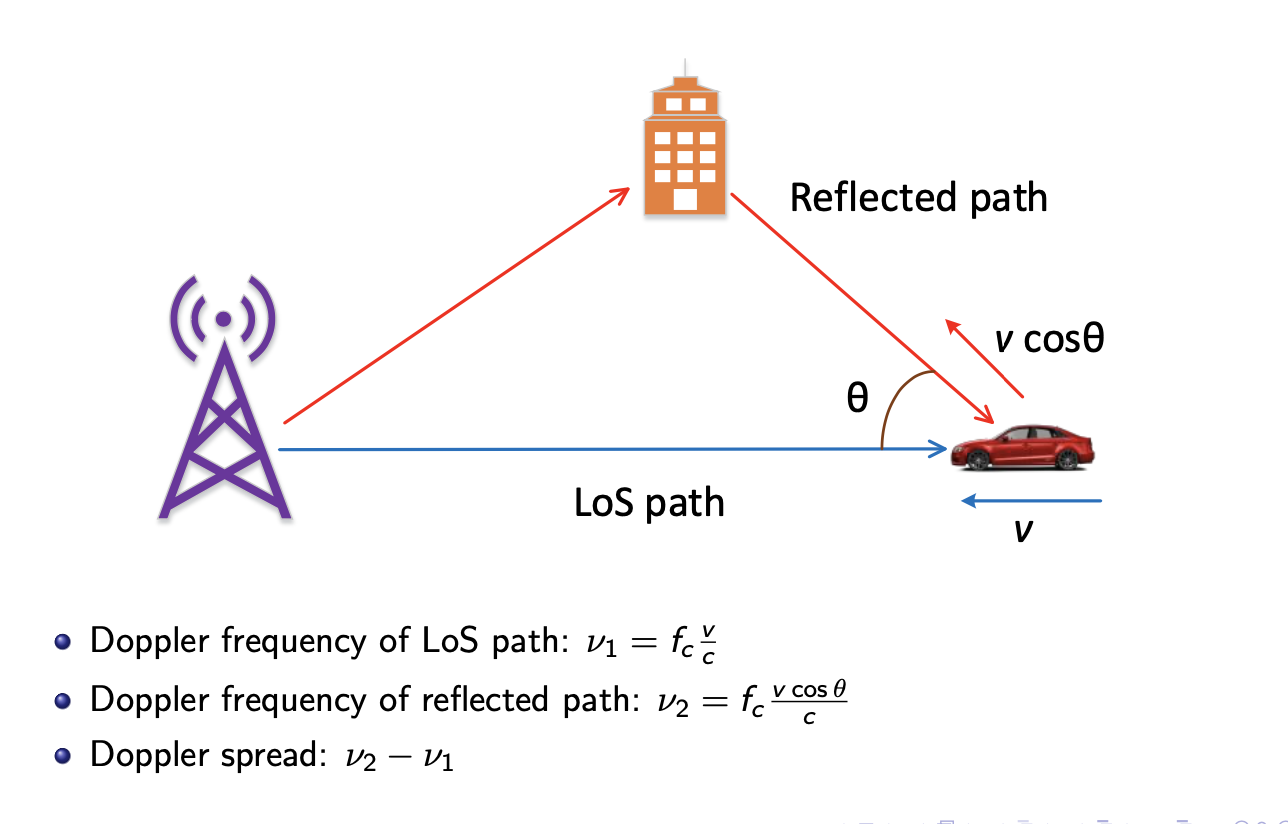
\includegraphics[width=0.82\textwidth]{Images/Chapter2/doppler_spread.png}
    \caption[Illustration of Doppler shift and Doppler spread in a wireless channel.]{Illustration of Doppler shift and Doppler spread in a wireless channel~\protect\cite{Hong2019OTFSTutorial}.}
    \label{fig:doppler_spread}
\end{figure}

Figure~\ref{fig:doppler_spread} illustrates the Doppler effect in a mobile wireless channel. For the LoS path, the motion is assumed to be aligned with the propagation direction, so the Doppler shift can be written as \(f_D=f_c v/c\). For the reflected path, only the velocity component along the propagation direction contributes to the Doppler shift, resulting in \(f_D=f_c v\cos\theta/c\). Since different propagation paths may arrive from different directions, they experience different Doppler shifts.

When multiple propagation paths are present, the received signal contains a range of Doppler shifts rather than a single frequency offset. This range is called Doppler spread. A small Doppler spread means that the channel varies slowly with time, while a large Doppler spread indicates a rapidly time-varying channel.

Doppler spread describes how much the received signal is spread in frequency due to motion. A small Doppler spread means that the channel varies slowly with time. A large Doppler spread means that the channel changes rapidly. Therefore, Doppler spread is closely related to time selectivity.

In low-mobility systems, the wireless channel may remain nearly constant over several symbol intervals. In this case, conventional channel estimation and equalization methods are usually effective. However, in high-mobility environments, the channel may change significantly during a transmission frame or even within one OFDM symbol. This rapid variation makes detection more difficult and may lead to serious performance degradation.

The Doppler effect is particularly important for OFDM systems. OFDM relies on the orthogonality among subcarriers. When the channel varies rapidly due to large Doppler spread, this orthogonality may be destroyed. As a result, energy from one subcarrier leaks into neighboring subcarriers, producing inter-carrier interference (ICI).

Table~\ref{tab:doppler_effects} summarizes the main effects of Doppler shift and Doppler spread.

\begin{table}[H]
\centering
\caption{Effects of Doppler shift and Doppler spread.}
\label{tab:doppler_effects}

\begin{tabular}{|p{4cm}|p{4cm}|p{5cm}|}
\hline
\textbf{Cause} &
\textbf{Channel Effect} &
\textbf{Main Consequence} \\
\hline

Relative motion &
Frequency shift of each path &
Doppler shift \\
\hline

Multiple moving paths &
Range of Doppler shifts &
Doppler spread \\
\hline

Large Doppler spread &
Rapid channel variation &
Time selectivity \\
\hline

Time-selective channel &
Loss of subcarrier orthogonality &
Inter-carrier interference \\
\hline

High mobility &
Fast time-varying channel response &
Difficult channel estimation and equalization \\
\hline

\end{tabular}

\end{table}

In summary, delay spread is mainly associated with multipath propagation, while Doppler spread is mainly associated with mobility. Delay spread causes frequency selectivity, whereas Doppler spread causes time selectivity. Both effects appear simultaneously in many practical high-mobility systems.

\subsubsection{Doubly Selective Channels}

A wireless channel is called doubly selective when it is both frequency selective and time selective. Frequency selectivity is caused by delay spread, while time selectivity is caused by Doppler spread. Therefore, doubly selective channels appear when multipath propagation and mobility occur simultaneously.

Doubly selective channels are common in high-mobility wireless communication scenarios. Examples include high-speed railways, vehicular networks, unmanned aerial vehicles, and low-earth-orbit satellite communications. In these scenarios, the transmitted signal experiences multiple propagation paths and rapid channel variation at the same time.

\begin{figure}[H]
    \centering

    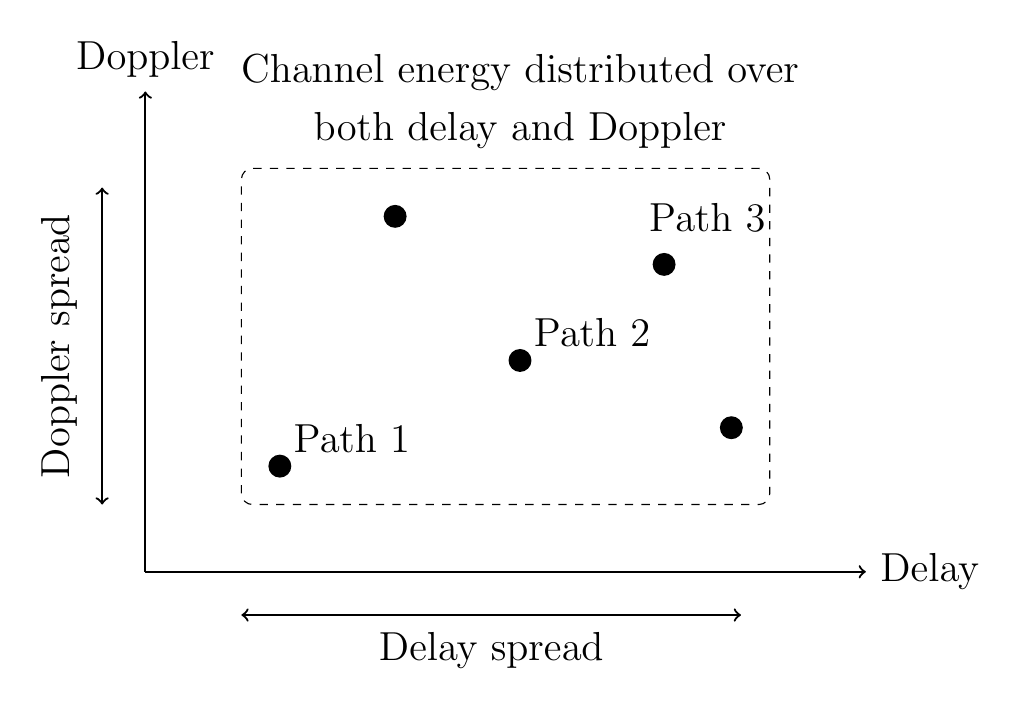
\begin{tikzpicture}[
        scale=1.22,
        transform shape,
        every node/.style={font=\small},
        axis/.style={->, thick},
        pathpoint/.style={circle, fill=black, inner sep=2.4pt},
        spread/.style={draw, dashed, rounded corners}
    ]

    % Axes
    \draw[axis] (0,0) -- (7.5,0) node[right] {Delay};
    \draw[axis] (0,0) -- (0,5.0) node[above] {Doppler};

    % Dashed area showing channel support
    \draw[spread] (1.0,0.7) rectangle (6.5,4.2);

    % Title inside the figure, moved away from y-axis label
    \node[align=center] at (3.9,4.9)
    {Channel energy distributed over\\both delay and Doppler};

    % Delay and Doppler spread indication
    \draw[<->, thick] (1.0,-0.45) -- (6.2,-0.45);
    \node at (3.6,-0.82) {Delay spread};

    \draw[<->, thick] (-0.45,0.7) -- (-0.45,4.0);
    \node[rotate=90] at (-0.9,2.35) {Doppler spread};

    % Path points
    \node[pathpoint] at (1.4,1.1) {};
    \node[pathpoint] at (2.6,3.7) {};
    \node[pathpoint] at (3.9,2.2) {};
    \node[pathpoint] at (5.4,3.2) {};
    \node[pathpoint] at (6.1,1.5) {};

    % Labels
    \node[above right] at (1.4,1.1) {Path 1};
    \node[above right] at (3.9,2.2) {Path 2};
    \node[above right] at (5.1,3.4) {Path 3};

    \end{tikzpicture}

    \caption{Conceptual illustration of a doubly selective channel with both delay and Doppler dispersion.}
    \label{fig:doubly_selective_channel}
\end{figure}

Figure~\ref{fig:doubly_selective_channel} conceptually illustrates a doubly selective channel. The delay dimension represents multipath-induced time dispersion, while the Doppler dimension represents mobility-induced frequency dispersion. Instead of being concentrated around a single propagation component, the channel energy is distributed across both delay and Doppler dimensions.

From a communication system perspective, doubly selective channels are difficult because they introduce both ISI and ICI. Delay spread may cause symbols to overlap in time, leading to ISI. Doppler spread may destroy subcarrier orthogonality, leading to ICI. When both effects are present, receiver design becomes significantly more challenging.

\begin{table}[H]
\centering
\caption{Relationship between propagation effects and channel selectivity.}
\label{tab:channel_selectivity}

\begin{tabular}{|p{4cm}|p{4cm}|p{5cm}|}
\hline
\textbf{Propagation Effect} &
\textbf{Channel Characteristic} &
\textbf{Resulting Impairment} \\
\hline

Delay spread &
Frequency selectivity &
Inter-symbol interference \\
\hline

Doppler spread &
Time selectivity &
Inter-carrier interference \\
\hline

Delay spread and Doppler spread &
Doubly selective channel &
ISI and ICI simultaneously \\
\hline

\end{tabular}

\end{table}

The concept of a doubly selective channel is central to the motivation of OTFS. OFDM can effectively deal with frequency-selective fading when the channel is approximately constant over one OFDM symbol. However, in high-Doppler environments, the channel changes rapidly and the simple diagonal subcarrier model of OFDM is no longer valid. This leads to significant performance degradation.

For this reason, waveform designs for future high-mobility communications must handle both delay and Doppler effects. OTFS addresses this problem by representing information symbols in the delay-Doppler domain, where the wireless channel can often be described more compactly in terms of physical propagation paths. Before discussing OTFS in detail, the next section reviews OFDM, which remains the dominant waveform in current wireless communication systems and provides a useful reference point for understanding the need for OTFS.


% ~8 pages
\subsection{Orthogonal Frequency Division Multiplexing}

Orthogonal Frequency Division Multiplexing (OFDM) has become the dominant waveform technology in modern wireless communication systems due to its high spectral efficiency and implementation simplicity. OFDM has been adopted in numerous communication standards, including LTE, 5G NR, Wi-Fi, and digital broadcasting systems. Before discussing the limitations of OFDM in high-mobility environments and the motivation for OTFS modulation, it is necessary to understand its fundamental operating principles.

\subsubsection{Principles of OFDM}

Orthogonal Frequency Division Multiplexing (OFDM) is a multicarrier transmission technique that divides a high-rate data stream into multiple parallel low-rate data streams. These streams are transmitted simultaneously over a set of orthogonal subcarriers, thereby reducing the symbol rate associated with each subcarrier and improving robustness against frequency-selective fading.

Unlike conventional Frequency Division Multiplexing (FDM), where adjacent subcarriers must be separated by guard bands to prevent interference, OFDM exploits the orthogonality between subcarriers to allow significant spectral overlap. As a result, OFDM achieves high spectral efficiency while maintaining the ability to separate individual subcarriers at the receiver.

The baseband OFDM signal can be expressed as

\begin{equation}
s(t)=\sum_{k=0}^{N-1} X_k e^{j2\pi k\Delta f t},
\quad 0 \le t < T
\end{equation}

where \(X_k\) denotes the complex symbol transmitted on the \(k\)-th subcarrier, \(N\) is the total number of subcarriers, and \(\Delta f\) represents the subcarrier spacing.

The key feature of OFDM is the orthogonality among subcarriers. Two subcarriers are orthogonal when

\begin{equation}
\int_{0}^{T}
e^{j2\pi n\Delta f t}
e^{-j2\pi m\Delta f t}
dt
=
0,
\quad n \neq m
\end{equation}

which is satisfied when the subcarrier spacing is chosen as

\begin{equation}
\Delta f = \frac{1}{T}
\end{equation}

where \(T\) denotes the OFDM symbol duration.

\begin{figure}[H]
    \centering
    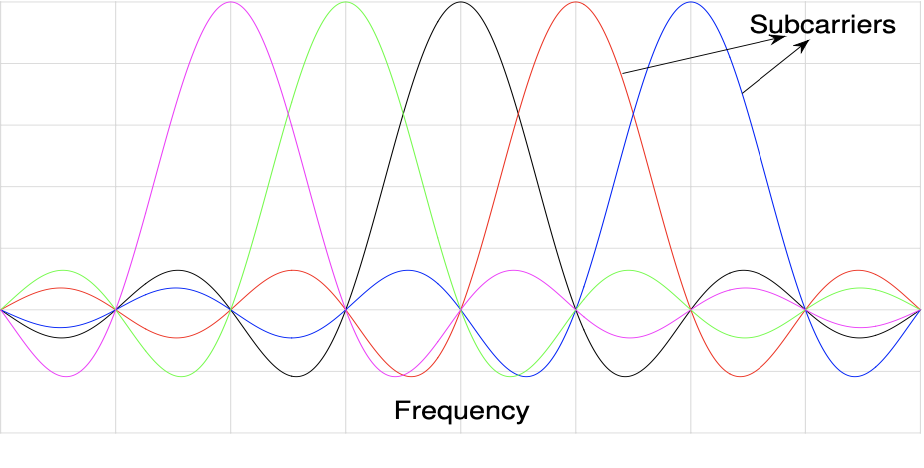
\includegraphics[width=1\textwidth]{Images/Chapter2/ofdmsubcarrier.png}
    \caption[Orthogonality among OFDM subcarriers.]{Orthogonality among OFDM subcarriers~\protect\cite{ScienceDirectICI}.}
    \label{fig:ofdm_orthogonality}
\end{figure}

As illustrated in Fig.~\ref{fig:ofdm_orthogonality}, the spectrum of each subcarrier exhibits a sinc-shaped response. Although adjacent subcarriers overlap significantly in the frequency domain, the peak of one subcarrier coincides with the null points of all other subcarriers. Consequently, mutual interference is avoided and the transmitted symbols can be recovered independently.

A major advantage of OFDM is its efficient implementation using the Inverse Fast Fourier Transform (IFFT) and Fast Fourier Transform (FFT). At the transmitter, information symbols are mapped onto frequency-domain subcarriers and transformed into the time domain using an IFFT operation. At the receiver, an FFT operation is applied to recover the transmitted symbols from the received waveform.

\begin{figure}[H]
    \centering
    \resizebox{0.95\textwidth}{!}{
    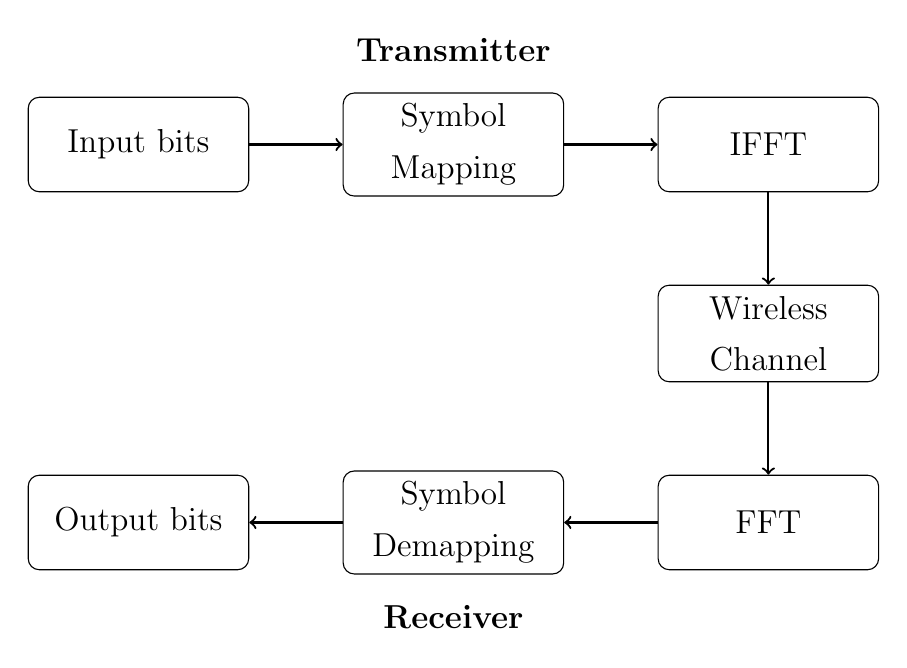
\begin{tikzpicture}[
        block/.style={
            draw,
            rounded corners,
            minimum width=2.8cm,
            minimum height=1.2cm,
            align=center,
            font=\normalsize
        },
        arrow/.style={->, thick}
    ]

    % =========================
    % Transmitter
    % =========================
    \node[block] (in)   at (0,2.4) {Input bits};
    \node[block] (map)  at (4.0,2.4) {Symbol\\Mapping};
    \node[block] (ifft) at (8.0,2.4) {IFFT};

    \draw[arrow] (in) -- (map);
    \draw[arrow] (map) -- (ifft);

    \node[font=\bfseries] at (4.0,3.6) {Transmitter};

    % =========================
    % Channel
    % =========================
    \node[block] (channel) at (8.0,0) {Wireless\\Channel};
    \draw[arrow] (ifft) -- (channel);

    % =========================
    % Receiver
    % =========================
    \node[block] (fft)   at (8.0,-2.4) {FFT};
    \node[block] (demap) at (4.0,-2.4) {Symbol\\Demapping};
    \node[block] (out)   at (0,-2.4) {Output bits};

    \draw[arrow] (channel) -- (fft);
    \draw[arrow] (fft) -- (demap);
    \draw[arrow] (demap) -- (out);

    \node[font=\bfseries] at (4.0,-3.6) {Receiver};

    \end{tikzpicture}
    }
    \caption{Basic principle of OFDM transmission using IFFT and FFT operations.}
    \label{fig:ofdm_basic_principle}
\end{figure}

By converting a broadband frequency-selective channel into multiple narrowband subchannels, OFDM significantly simplifies receiver design and equalization. This property has contributed to its widespread adoption in modern wireless communication systems. However, despite these advantages, OFDM experiences considerable performance degradation in rapidly time-varying channels, particularly under high Doppler conditions. These limitations are discussed in the following subsections.


\subsubsection{OFDM Transceiver Structure}

The practical implementation of OFDM systems is based on digital signal processing techniques that efficiently generate and recover orthogonal subcarriers using IFFT and FFT operations. Instead of using a large number of separate oscillators and modulators for different subcarriers, OFDM generates all subcarriers jointly through an inverse Fourier transform. This significantly reduces implementation complexity while maintaining high spectral efficiency.

A typical OFDM transceiver consists of a transmitter, a wireless propagation channel, and a receiver. At the transmitter, the input binary data stream is first converted into parallel data streams. These bits are then mapped into complex modulation symbols using modulation schemes such as BPSK, QPSK, or QAM. The resulting symbols are assigned to different frequency-domain subcarriers.

To generate the time-domain OFDM waveform, an \(N\)-point Inverse Fast Fourier Transform (IFFT) is applied to the frequency-domain symbols. The IFFT converts the parallel subcarrier symbols into a discrete-time OFDM signal while preserving the orthogonality among subcarriers. The transmitted OFDM symbol can be expressed as

\begin{equation}
x[n]
=
\frac{1}{\sqrt{N}}
\sum_{k=0}^{N-1}
X[k]
e^{j\frac{2\pi kn}{N}},
\quad n=0,1,\ldots,N-1,
\end{equation}

where \(X[k]\) denotes the modulation symbol transmitted on the \(k\)-th subcarrier and \(N\) represents the total number of subcarriers.

In practical OFDM systems, a cyclic prefix (CP) is often appended to each OFDM symbol before transmission. The CP is formed by copying the last portion of the OFDM symbol and inserting it at the beginning of the symbol interval. This operation helps mitigate inter-symbol interference (ISI) caused by multipath propagation and allows the linear convolution of the channel to be treated approximately as circular convolution. As a result, frequency-domain equalization at the receiver becomes much simpler.

\begin{figure}[H]
    \centering
    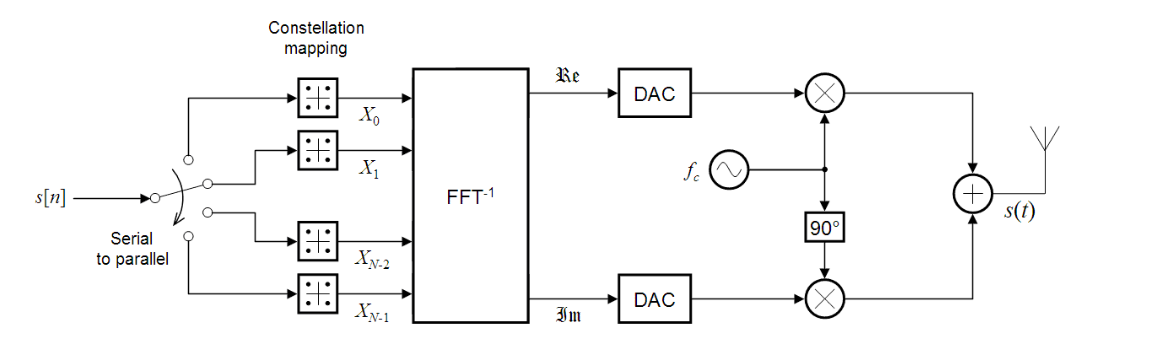
\includegraphics[width=0.92\textwidth]{Images/Chapter2/ofdmtx.png}
    \caption[OFDM transmitter structure.]{OFDM transmitter structure~\protect\cite{Hong2019OTFSTutorial}.}
    \label{fig:ofdm_tx}
\end{figure}

\begin{figure}[H]
    \centering
    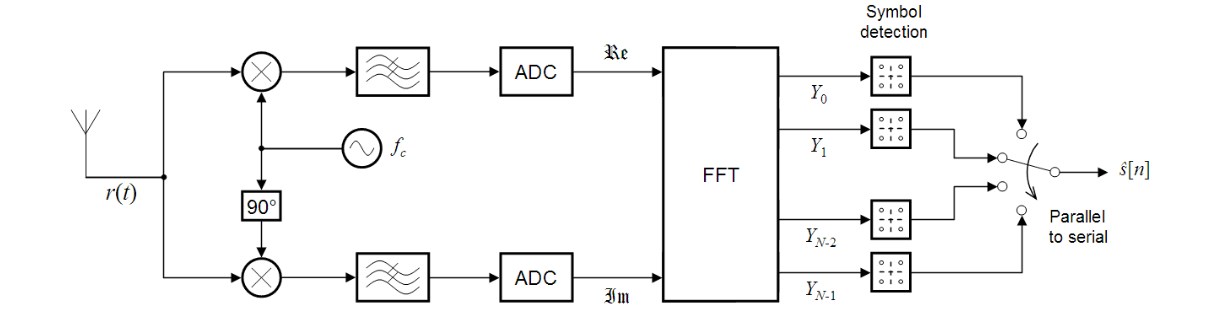
\includegraphics[width=0.92\textwidth]{Images/Chapter2/ofdmrx.png}
    \caption[OFDM receiver structure.]{OFDM receiver structure~\protect\cite{Hong2019OTFSTutorial}.}
    \label{fig:ofdm_rx}
\end{figure}



As illustrated in Fig.~\ref{fig:ofdm_tx}, the transmitter performs serial-to-parallel conversion, constellation mapping, IFFT processing, digital-to-analog conversion, and carrier modulation before radiating the signal through the antenna. The IFFT block is the key baseband processing stage because it converts frequency-domain subcarrier symbols into a time-domain waveform suitable for transmission.

After propagating through the wireless channel, the received signal is affected by multipath fading, Doppler shifts, and additive noise. At the receiver, the signal is first downconverted from the carrier frequency, filtered, and converted back into digital samples. The FFT operation is then applied to transform the received time-domain signal back into the frequency domain. Symbol detection and parallel-to-serial conversion are finally performed to recover the estimated transmitted bit sequence.

Under the assumption that the channel remains approximately constant during one OFDM symbol interval and that the CP is sufficiently long, the received symbol on the \(k\)-th subcarrier can be represented as

\begin{equation}
Y[k]
=
H[k]X[k]
+
W[k],
\end{equation}

where \(Y[k]\) is the received symbol on the \(k\)-th subcarrier, \(H[k]\) denotes the channel frequency response, \(X[k]\) is the transmitted symbol, and \(W[k]\) represents the noise component.

Because each OFDM subcarrier experiences an approximately flat channel response, equalization can be performed independently for each subcarrier. This one-tap frequency-domain equalization greatly reduces receiver complexity compared with single-carrier systems operating over frequency-selective channels.

The use of FFT-based processing and simple per-subcarrier equalization is one of the main reasons for the widespread adoption of OFDM in modern wireless communication systems. However, these advantages rely on the assumption that the channel is nearly time-invariant within each OFDM symbol. In high-mobility environments, Doppler spread causes rapid channel variation and may destroy the orthogonality among subcarriers, resulting in inter-carrier interference and degraded system performance.


\subsubsection{Advantages of OFDM}

OFDM has been widely adopted in modern wireless communication systems because it provides an efficient solution for transmission over frequency-selective fading channels. By dividing a wideband channel into a large number of narrowband orthogonal subchannels, OFDM simplifies the equalization problem and enables reliable high-data-rate transmission.

One of the most important advantages of OFDM is its robustness against multipath propagation. In a single-carrier system, multipath delay spread may cause severe inter-symbol interference because delayed replicas of previous symbols overlap with the current symbol. In OFDM, the symbol duration on each subcarrier is increased by transmitting data in parallel over many subcarriers. As a result, the relative impact of delay spread is reduced.

Another major advantage is the use of the cyclic prefix. When the cyclic prefix length is longer than the maximum delay spread of the channel, the linear convolution between the transmitted signal and the multipath channel can be transformed into circular convolution. This allows the frequency-selective channel to be represented as a set of parallel flat-fading subchannels after the FFT operation at the receiver.

Under ideal synchronization and sufficiently slow channel variation, the received signal on each subcarrier follows the one-tap input-output relation introduced in the previous subsection. Since the transmitted symbols are separated in the frequency domain, each subcarrier can be equalized independently using a one-tap equalizer.

The estimated transmitted symbol can therefore be obtained as

\begin{equation}
\hat{X}[k]=\frac{Y[k]}{H[k]},
\end{equation}

where \(H[k]\) is the channel frequency response on the \(k\)-th subcarrier.

This one-tap frequency-domain equalization is one of the key reasons for the practical success of OFDM. Compared with time-domain equalization in wideband single-carrier systems, OFDM significantly reduces receiver complexity.

\begin{figure}[H]
    \centering
    \resizebox{0.95\textwidth}{!}{
    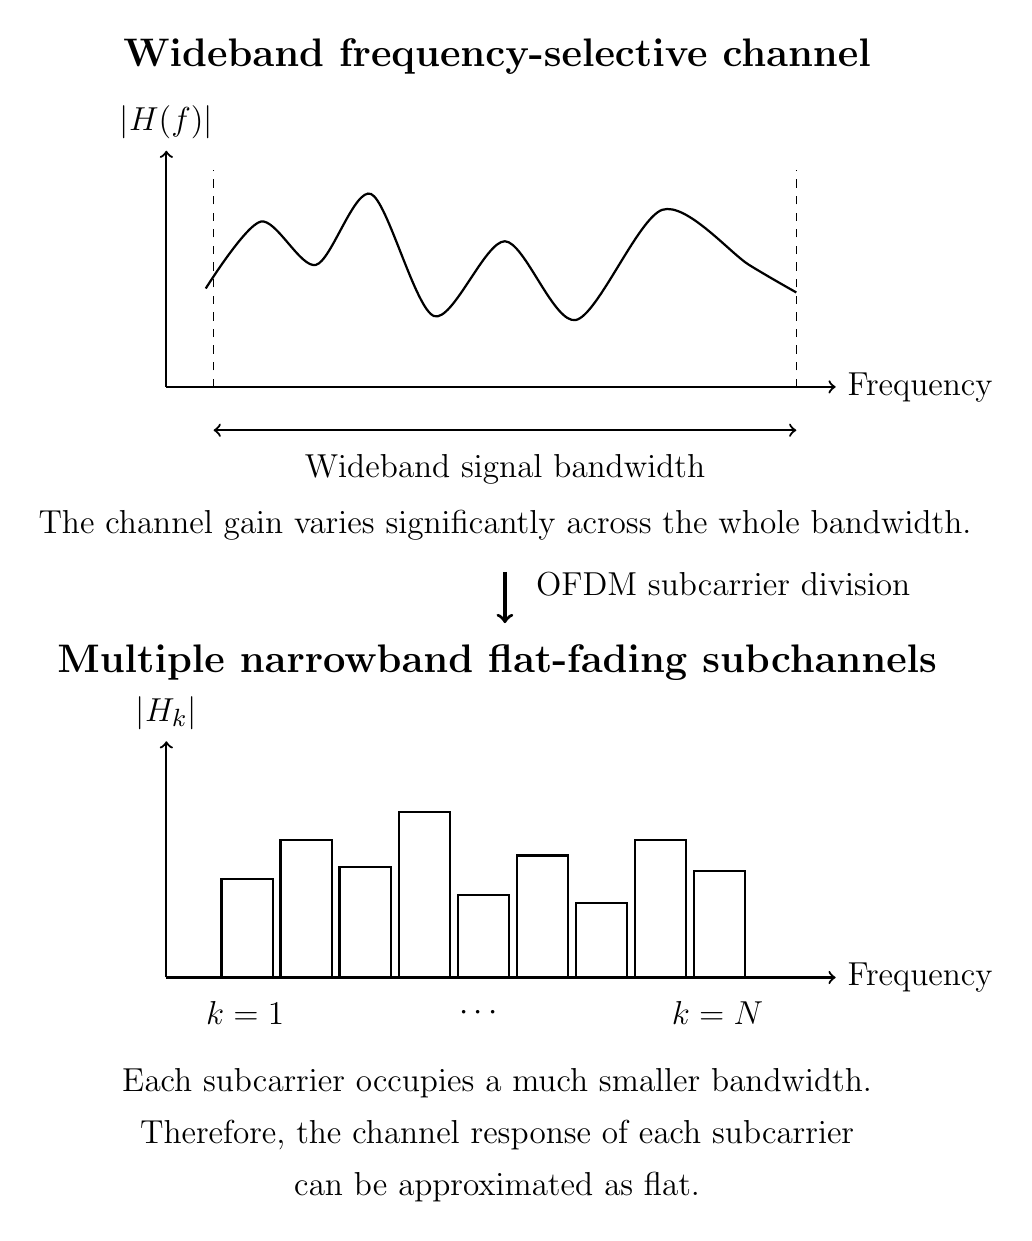
\begin{tikzpicture}[
        every node/.style={font=\normalsize},
        axis/.style={->, thick},
        thickline/.style={thick}
    ]

    % =====================================================
    % Top: Wideband frequency-selective channel
    % =====================================================
    \node[font=\bfseries\large] at (4.2,4.2)
    {Wideband frequency-selective channel};

    \draw[axis] (0,0) -- (8.5,0) node[right] {Frequency};
    \draw[axis] (0,0) -- (0,3.0) node[above] {$|H(f)|$};

    % Frequency-selective response
    \draw[thickline]
        plot[smooth] coordinates {
        (0.5,1.25)
        (1.2,2.10)
        (1.9,1.55)
        (2.6,2.45)
        (3.4,0.90)
        (4.3,1.85)
        (5.2,0.85)
        (6.3,2.25)
        (7.4,1.55)
        (8.0,1.20)
        };

    % Bandwidth marks
    \draw[dashed] (0.6,0) -- (0.6,2.75);
    \draw[dashed] (8.0,0) -- (8.0,2.75);

    \draw[<->, thick] (0.6,-0.55) -- (8.0,-0.55);
    \node at (4.3,-1.05) {Wideband signal bandwidth};

    % Explanation label
    \node[align=center] at (4.3,-1.75)
    {The channel gain varies significantly across the whole bandwidth.};

    % =====================================================
    % Down arrow
    % =====================================================
    \draw[->, very thick] (4.3,-2.35) -- (4.3,-3.0);
    \node[right] at (4.55,-2.5) {OFDM subcarrier division};

    % =====================================================
    % Bottom: Narrowband subchannels
    % =====================================================
    \begin{scope}[yshift=-7.5cm]

    \node[font=\bfseries\large] at (4.2,4.0)
    {Multiple narrowband flat-fading subchannels};

    \draw[axis] (0,0) -- (8.5,0) node[right] {Frequency};
    \draw[axis] (0,0) -- (0,3.0) node[above] {$|H_k|$};

    % Draw narrow flat subchannels
    \draw[thick] (0.7,0) rectangle (1.35,1.25);
    \draw[thick] (1.45,0) rectangle (2.10,1.75);
    \draw[thick] (2.20,0) rectangle (2.85,1.40);
    \draw[thick] (2.95,0) rectangle (3.60,2.10);
    \draw[thick] (3.70,0) rectangle (4.35,1.05);
    \draw[thick] (4.45,0) rectangle (5.10,1.55);
    \draw[thick] (5.20,0) rectangle (5.85,0.95);
    \draw[thick] (5.95,0) rectangle (6.60,1.75);
    \draw[thick] (6.70,0) rectangle (7.35,1.35);

    % Labels
    \node at (1.0,-0.45) {$k=1$};
    \node at (4.0,-0.45) {$\cdots$};
    \node at (7.0,-0.45) {$k=N$};

    \node[align=center] at (4.2,-2)
    {Each subcarrier occupies a much smaller bandwidth.\\
    Therefore, the channel response of each subcarrier\\
    can be approximated as flat.};

    \end{scope}

    \end{tikzpicture}
    }

    \caption{Conversion of a frequency-selective wideband channel into multiple narrowband flat-fading subchannels in OFDM.}
    \label{fig:ofdm_parallel_subchannels}
\end{figure}


OFDM also provides high spectral efficiency due to the orthogonality among subcarriers. Unlike conventional frequency division multiplexing, which requires guard bands between adjacent carriers, OFDM allows subcarrier spectra to overlap while still avoiding mutual interference under ideal conditions. This property makes OFDM particularly suitable for bandwidth-limited wireless communication systems.

The main advantages of OFDM are summarized in Table~\ref{tab:ofdm_advantages}.

\begin{table}[H]
\centering
\caption{Main advantages of OFDM systems.}
\label{tab:ofdm_advantages}

\begin{tabular}{|p{4cm}|p{8cm}|}
\hline
\textbf{Advantage} &
\textbf{Description} \\
\hline

High spectral efficiency &
Overlapping orthogonal subcarriers reduce the need for guard bands. \\
\hline

Robustness to multipath &
Longer symbol duration and cyclic prefix reduce the effect of delay spread. \\
\hline

Simple equalization &
Frequency-selective channels are transformed into parallel flat-fading subchannels. \\
\hline

FFT-based implementation &
IFFT and FFT operations enable efficient digital implementation. \\
\hline

Flexible resource allocation &
Subcarriers can be assigned adaptively according to channel conditions and user requirements. \\
\hline

\end{tabular}

\end{table}

Despite these advantages, OFDM relies heavily on the preservation of subcarrier orthogonality. This requirement becomes difficult to satisfy in rapidly time-varying wireless channels, especially when the receiver operates under high mobility. The limitations of OFDM under such conditions are discussed in the following subsection.

\subsubsection{Limitations of OFDM in High-Mobility Environments}

Although OFDM is highly effective in combating frequency-selective fading, its performance can degrade significantly in high-mobility environments. The main reason is that OFDM assumes the wireless channel remains approximately constant during one OFDM symbol duration. When this assumption is violated, the orthogonality among subcarriers is destroyed.

In high-mobility scenarios, relative motion between the transmitter, receiver, and scatterers introduces Doppler shifts. These Doppler shifts cause the channel response to vary within an OFDM symbol interval. Consequently, the received signal is no longer affected only by the channel gain on its own subcarrier, but also by leakage from neighboring subcarriers. This phenomenon is known as inter-carrier interference (ICI).

Under ideal conditions, the received signal on the \(k\)-th subcarrier is represented by

\begin{equation}
Y[k]=H[k]X[k]+W[k].
\end{equation}

However, in the presence of Doppler-induced channel variation, the received signal becomes

\begin{equation}
Y[k]=H[k]X[k]+\sum_{\substack{m=0 \\ m\neq k}}^{N-1} I[k,m]X[m]+W[k],
\end{equation}

where \(I[k,m]\) represents the interference contribution from the \(m\)-th subcarrier to the \(k\)-th subcarrier. The second term in the equation represents inter-carrier interference caused by the loss of orthogonality.

\begin{figure}[H]
    \centering
    
\includegraphics[width=1\textwidth]{Images/Chapter2/ici.png}
    \caption[Inter-carrier interference in OFDM caused by Doppler-induced loss of subcarrier orthogonality.]{Inter-carrier interference in OFDM caused by Doppler-induced loss of subcarrier orthogonality~\protect\cite{Hong2019OTFSTutorial}.}
    \label{fig:ofdm_ici}
\end{figure}

As illustrated in Fig.~\ref{fig:ofdm_ici}, Doppler shifts disturb the frequency-domain alignment of OFDM subcarriers. The null points of one subcarrier no longer coincide with the peaks of other subcarriers, causing interference among subcarriers. This effect becomes more severe as the Doppler spread increases.

Another limitation of OFDM is that the performance of the system is strongly affected by the weakest subcarriers. In a frequency-selective fading channel, some subcarriers may experience deep fading while others maintain strong channel gains. Although coding and interleaving can mitigate this problem to some extent, the overall reliability of the system may still be limited by poorly conditioned subchannels.

Furthermore, the one-tap equalization structure of OFDM is only effective when the channel matrix remains nearly diagonal in the frequency domain. In high-Doppler conditions, the channel matrix loses this diagonal structure due to ICI. Equalization therefore becomes more complex, and the simplicity that makes OFDM attractive is partially lost.

\begin{table}[H]
\centering
\caption{Main limitations of OFDM in high-mobility environments.}
\label{tab:ofdm_limitations}

\begin{tabular}{|p{4cm}|p{8cm}|}
\hline
\textbf{Limitation} &
\textbf{Impact} \\
\hline

Sensitivity to Doppler spread &
Doppler shifts destroy subcarrier orthogonality and introduce ICI. \\
\hline

Channel time variation &
The channel may change within one OFDM symbol, violating the quasi-static channel assumption. \\
\hline

Deep fading on subcarriers &
Some subcarriers may experience severe attenuation, reducing reliability. \\
\hline

Increased equalization complexity &
The channel matrix is no longer diagonal under severe Doppler conditions. \\
\hline

Performance degradation in high mobility &
BER increases significantly in vehicular, high-speed railway, UAV, and satellite communication scenarios. \\
\hline

\end{tabular}

\end{table}

These limitations motivate the search for alternative waveform designs that can better handle doubly selective channels. Instead of representing information symbols only in the time-frequency domain, OTFS modulation introduces a delay-Doppler domain representation where the channel can be described more compactly and more stably under high mobility. Before introducing OTFS in detail, the next section reviews the delay-Doppler domain representation of wireless channels.


\subsection{Delay-Doppler Domain Representation}

The analysis of high-mobility wireless channels requires a signal representation that can describe both multipath propagation and Doppler effects. Conventional multicarrier systems such as OFDM usually describe signal transmission in the time-frequency domain. This representation is convenient for practical implementation, because data symbols can be arranged over time slots and frequency subcarriers.

However, in high-mobility environments, the wireless channel may vary rapidly over time due to Doppler effects. As a result, the time-frequency channel coefficients can change significantly from one resource element to another. This makes channel estimation and equalization more difficult. For this reason, the delay-Doppler domain is introduced as an alternative representation that is more closely related to the physical propagation paths of the wireless channel.

The delay-Doppler representation is an important foundation for OTFS modulation. Instead of describing the channel only by its variations over time and frequency, this representation describes the channel using propagation delay and Doppler shift. These two quantities correspond directly to multipath propagation and relative motion, respectively.

\subsubsection{Time-Frequency Domain}

The time-frequency domain is widely used in modern wireless communication systems, especially in OFDM-based transmission. In this representation, the available transmission resources are divided into time slots and frequency subcarriers. Each information symbol is placed on a specific time-frequency resource element.

The time axis represents consecutive OFDM symbols or time slots, while the frequency axis represents the orthogonal subcarriers. Therefore, each cell in the time-frequency grid corresponds to one symbol position in both time and frequency. This structure is suitable for OFDM because one OFDM symbol occupies a time interval and contains multiple subcarriers in the frequency domain.

\begin{figure}[H]
\centering
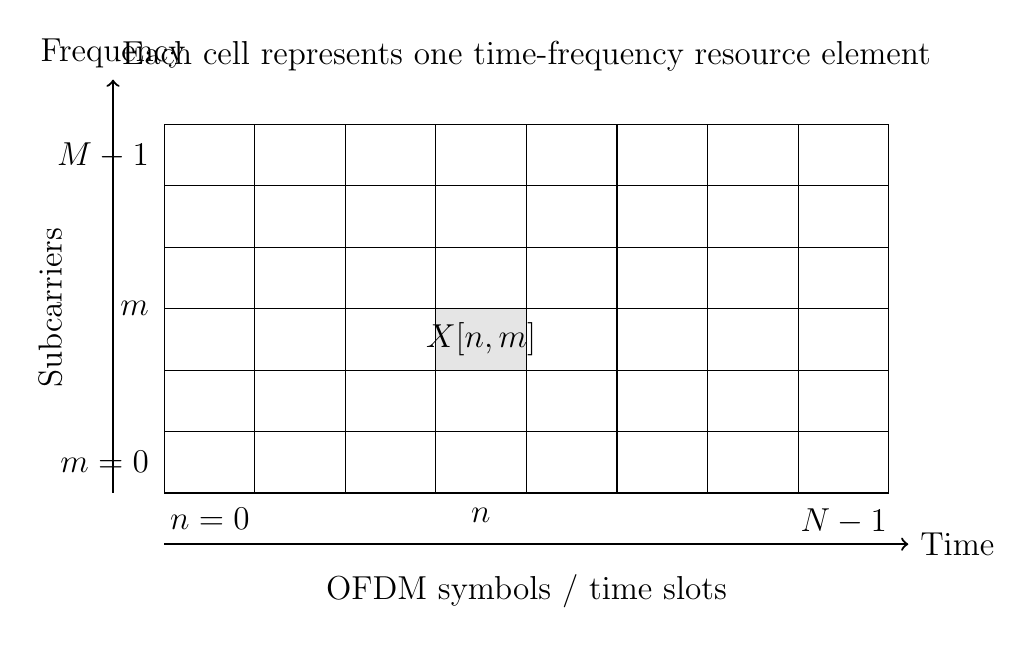
\begin{tikzpicture}[every node/.style={font=\small}]

    % Grid parameters
    \def\cw{1.15}
    \def\ch{0.78}

    % Draw grid
    \foreach \i in {0,...,7} {
        \foreach \j in {0,...,5} {
            \draw (\i*\cw,\j*\ch) rectangle ++(\cw,\ch);
        }
    }

    % Highlight one resource element
    \filldraw[fill=gray!20, draw=black] (3*\cw,2*\ch) rectangle ++(\cw,\ch);
    \node at (3*\cw+0.5*\cw,2*\ch+0.5*\ch) {$X[n,m]$};

    % Axes
    \draw[->, thick] (-0.65,0) -- (-0.65,5.25) node[above] {Frequency};
    \draw[->, thick] (0,-0.65) -- (9.45,-0.65) node[right] {Time};

    % Axis descriptors
    \node[rotate=90] at (-1.45,2.35) {Subcarriers};
    \node at (4.6,-1.25) {OFDM symbols / time slots};

    % Labels on vertical axis
    \node[left] at (-0.05,0.39) {$m=0$};
    \node[left] at (-0.05,2.34) {$m$};
    \node[left] at (-0.05,4.29) {$M-1$};

    % Labels on horizontal axis
    \node[below] at (0.58,-0.05) {$n=0$};
    \node[below] at (4.02,-0.05) {$n$};
    \node[below] at (8.63,-0.05) {$N-1$};

    % Top explanation
    \node at (4.6,5.55) {Each cell represents one time-frequency resource element};

\end{tikzpicture}
\caption{Time-frequency grid representation used in multicarrier transmission systems.}
\label{fig:time_frequency_grid}

\end{figure}

Figure~\ref{fig:time_frequency_grid} illustrates the time-frequency grid structure. In OFDM, data symbols are directly assigned to this grid. The receiver then processes the received signal in the frequency domain using FFT-based operations. This approach is effective when the channel is approximately constant during one OFDM symbol interval.

Nevertheless, the time-frequency representation becomes less stable in high-mobility environments. When the transmitter, receiver, or surrounding scatterers move rapidly, the channel changes during transmission. Consequently, the channel response in the time-frequency domain may fluctuate quickly across both time and frequency. This effect can destroy the orthogonality among OFDM subcarriers and introduce inter-carrier interference.

Although the time-frequency domain is convenient for waveform generation and practical implementation, it does not always provide the most compact description of doubly selective channels. This motivates the use of the delay-Doppler domain.

\subsubsection{Delay-Doppler Representation}

The delay-Doppler domain describes the wireless channel using two physical parameters: propagation delay and Doppler shift. The delay dimension is associated with multipath propagation. Different reflected paths travel different distances before reaching the receiver, so they arrive at different times. The Doppler dimension is associated with relative motion. When the transmitter, receiver, or scatterers are moving, each path may experience a frequency shift.

In this representation, each dominant propagation path can be described by three main parameters: its path gain, its delay, and its Doppler shift. Therefore, instead of viewing the channel as a rapidly changing surface over time and frequency, the delay-Doppler domain views it as a collection of physical propagation paths.

A simple delay-Doppler channel model can be expressed as

\begin{equation}
h(\tau,\nu)
=
\sum_{i=1}^{P}
h_i
\delta(\tau-\tau_i)
\delta(\nu-\nu_i),
\end{equation}

where \(P\) denotes the number of dominant propagation paths. The parameter \(h_i\) represents the complex gain of the \(i\)-th path, while \(\tau_i\) and \(\nu_i\) denote its delay and Doppler shift, respectively.

This equation means that the channel can be interpreted as the sum of several dominant propagation components. Each component appears at a certain delay and a certain Doppler shift. In many practical wireless channels, only a limited number of propagation paths carry significant energy. Therefore, the delay-Doppler channel representation is often sparse.

\begin{figure}[H]
\centering
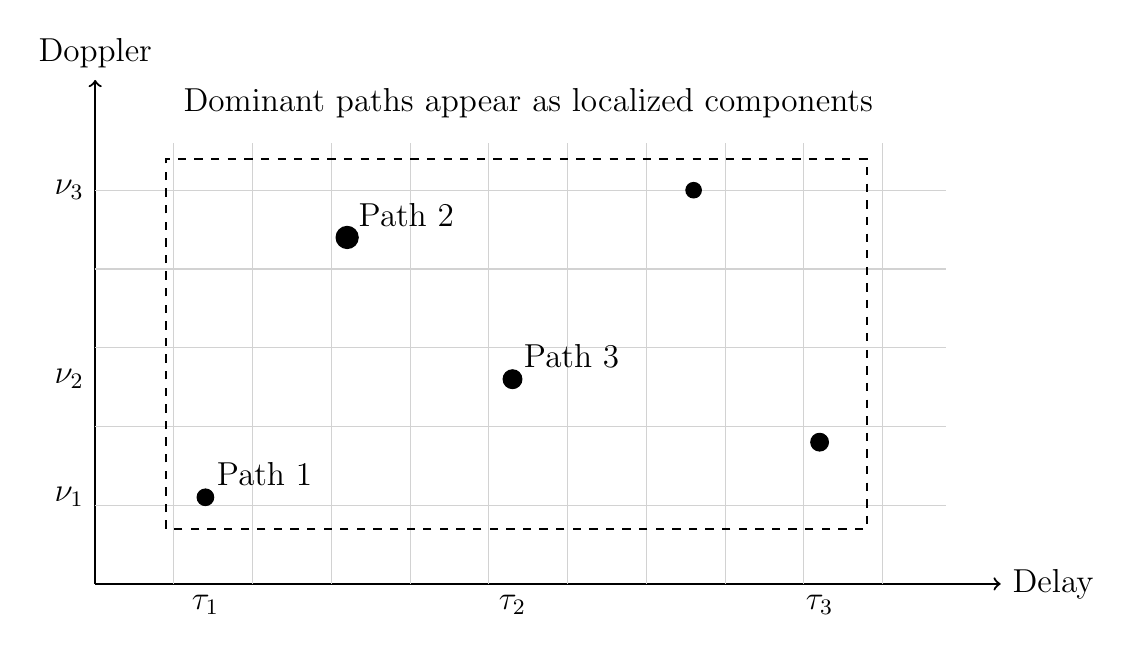
\begin{tikzpicture}[
every node/.style={font=\small},
axis/.style={->, thick},
gridline/.style={gray!35, thin}
]

    % Axes
    \draw[axis] (0,0) -- (11.5,0) node[right] {Delay};
    \draw[axis] (0,0) -- (0,6.4) node[above] {Doppler};

    % Grid
    \foreach \x in {1,2,...,10} {
        \draw[gridline] (\x,0) -- (\x,5.6);
    }

    \foreach \y in {1,2,3,4,5} {
        \draw[gridline] (0,\y) -- (10.8,\y);
    }

    % Sparse dominant paths
    \filldraw[black] (1.4,1.1) circle (3.0pt);
    \filldraw[black] (3.2,4.4) circle (4.0pt);
    \filldraw[black] (5.3,2.6) circle (3.4pt);
    \filldraw[black] (7.6,5.0) circle (2.8pt);
    \filldraw[black] (9.2,1.8) circle (3.2pt);

    % Path labels
    \node[above right] at (1.4,1.1) {Path 1};
    \node[above right] at (3.2,4.4) {Path 2};
    \node[above right] at (5.3,2.6) {Path 3};

    % Sparse support region
    \draw[dashed, thick] (0.9,0.7) rectangle (9.8,5.4);

    % Axis tick labels
    \node[below] at (1.4,0) {$\tau_1$};
    \node[below] at (5.3,0) {$\tau_2$};
    \node[below] at (9.2,0) {$\tau_3$};

    \node[left] at (0,1.1) {$\nu_1$};
    \node[left] at (0,2.6) {$\nu_2$};
    \node[left] at (0,5.0) {$\nu_3$};

    % Annotation
    \node[align=center] at (5.5,6.1)
    {Dominant paths appear as localized components};

\end{tikzpicture}
\caption{Sparse representation of dominant multipath components in the delay-Doppler domain.}
\label{fig:delay_doppler_channel}

\end{figure}

As illustrated in Fig.~\ref{fig:delay_doppler_channel}, each significant propagation path appears as a localized component in the delay-Doppler plane. The horizontal coordinate represents the propagation delay, while the vertical coordinate represents the Doppler shift. Since the number of dominant paths is usually limited, the channel energy is concentrated around several points or small regions.

This sparse representation is useful in high-mobility communications. In the time-frequency domain, the channel coefficients may vary rapidly due to Doppler effects. In the delay-Doppler domain, however, the physical path parameters usually vary more slowly. This makes the delay-Doppler domain more suitable for describing doubly selective wireless channels.

Compared with the time-frequency domain, the delay-Doppler domain provides a more compact and physically meaningful description of the wireless channel. This is one of the main motivations for OTFS modulation.

\subsubsection{Relationship Between Signal Domains}

The time-frequency and delay-Doppler domains are not independent representations. They describe the same wireless communication system from different viewpoints. The time-frequency domain is convenient for practical waveform generation, while the delay-Doppler domain is more suitable for describing physical channel behavior in high-mobility scenarios.

In conventional OFDM systems, information symbols are placed directly on the time-frequency grid. Each symbol is associated with a particular OFDM symbol index and subcarrier index. In contrast, OTFS places information symbols on the delay-Doppler grid first. These symbols are then transformed into the time-frequency grid before transmission.

This transformation is performed by the inverse symplectic finite Fourier transform (ISFFT). At the receiver, after the signal has passed through the wireless channel and has been processed in the time-frequency domain, the symplectic finite Fourier transform (SFFT) is used to transform the received samples back into the delay-Doppler domain.

Instead of presenting the full mathematical expressions of these transforms here, the main idea can be understood as follows. The ISFFT spreads each delay-Doppler symbol over the time-frequency plane before transmission. After reception, the SFFT collects the received time-frequency information back into the delay-Doppler domain. Therefore, the two transforms form a bridge between the physical delay-Doppler representation and the practical time-frequency transmission structure.

\begin{figure}[H]
\centering
\resizebox{0.96\linewidth}{!}{%
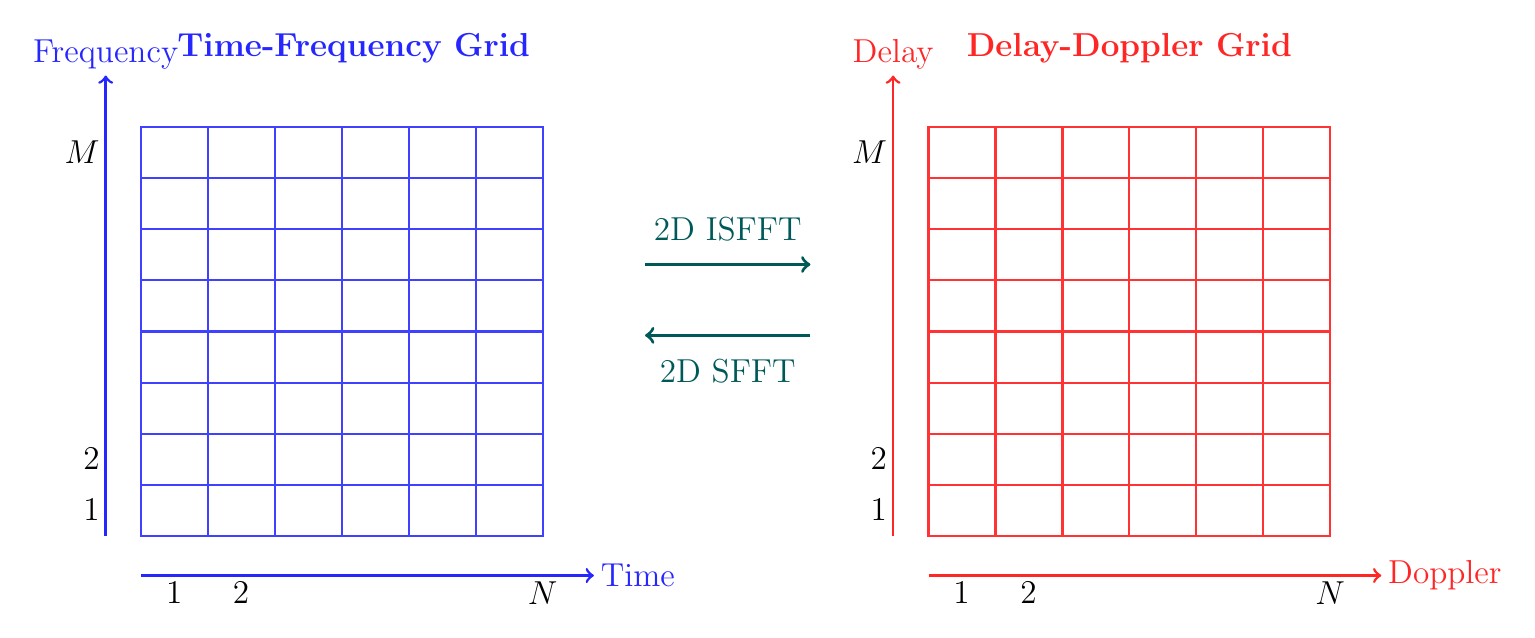
\begin{tikzpicture}[every node/.style={font=\small, inner sep=2pt}]

    % Parameters
    \def\cw{0.85}
    \def\ch{0.65}

    % =====================================================
    % Left grid: Time-Frequency
    % =====================================================
    \begin{scope}[shift={(0,0)}]

        \foreach \i in {0,...,5} {
            \foreach \j in {0,...,7} {
                \draw[blue!75, line width=0.8pt] (\i*\cw,\j*\ch) rectangle ++(\cw,\ch);
            }
        }

        \draw[->, blue!85, line width=1pt] (-0.45,0) -- (-0.45,5.85) node[above] {Frequency};
        \draw[->, blue!85, line width=1pt] (0,-0.5) -- (5.75,-0.5) node[right] {Time};

        \node[below] at (0.42,-0.5) {$1$};
        \node[below] at (1.27,-0.5) {$2$};
        \node[below] at (5.10,-0.5) {$N$};

        \node[left] at (-0.45,0.33) {$1$};
        \node[left] at (-0.45,0.98) {$2$};
        \node[left] at (-0.45,4.88) {$M$};

        \node[blue!85, font=\bfseries] at (2.7,6.2) {Time-Frequency Grid};

    \end{scope}

    % =====================================================
    % Middle arrows
    % =====================================================
    \draw[->, teal!70!black, line width=1.2pt] (6.4,3.45) -- (8.5,3.45);
    \node[teal!70!black] at (7.45,3.9) {2D ISFFT};

    \draw[->, teal!70!black, line width=1.2pt] (8.5,2.55) -- (6.4,2.55);
    \node[teal!70!black] at (7.45,2.1) {2D SFFT};

    % =====================================================
    % Right grid: Delay-Doppler
    % =====================================================
    \begin{scope}[shift={(10.0,0)}]

        \foreach \i in {0,...,5} {
            \foreach \j in {0,...,7} {
                \draw[red!80, line width=0.8pt] (\i*\cw,\j*\ch) rectangle ++(\cw,\ch);
            }
        }

        \draw[->, red!85, line width=1pt] (-0.45,0) -- (-0.45,5.85) node[above] {Delay};
        \draw[->, red!85, line width=1pt] (0,-0.5) -- (5.75,-0.5) node[right] {Doppler};

        \node[below] at (0.42,-0.5) {$1$};
        \node[below] at (1.27,-0.5) {$2$};
        \node[below] at (5.10,-0.5) {$N$};

        \node[left] at (-0.45,0.33) {$1$};
        \node[left] at (-0.45,0.98) {$2$};
        \node[left] at (-0.45,4.88) {$M$};

        \node[red!85, font=\bfseries] at (2.55,6.2) {Delay-Doppler Grid};

    \end{scope}

\end{tikzpicture}
}
\caption{Relationship between time-frequency and delay-Doppler signal domains.}
\label{fig:tf_dd_relationship}

\end{figure}

As illustrated in Fig.~\ref{fig:tf_dd_relationship}, the delay-Doppler grid and the time-frequency grid are connected through two-dimensional transforms. The delay-Doppler grid is useful for symbol placement and channel interpretation, while the time-frequency grid is suitable for practical transmission using multicarrier waveforms.

This relationship is particularly important for OTFS. OTFS does not completely discard the time-frequency domain. Instead, it uses the delay-Doppler domain for data representation and then maps the symbols into the time-frequency domain for transmission. In this way, OTFS can remain compatible with multicarrier transmission principles while exploiting the physical delay and Doppler characteristics of high-mobility wireless channels.

Table~\ref{tab:signal_domain_relationship} summarizes the main differences between the two domains.

\begin{table}[H]
\centering
\caption{Comparison between time-frequency and delay-Doppler signal domains.}
\label{tab:signal_domain_relationship}

\renewcommand{\arraystretch}{1.35}
\begin{tabularx}{\textwidth}{|
>{\RaggedRight\arraybackslash}p{3.0cm}|
>{\RaggedRight\arraybackslash}X|
>{\RaggedRight\arraybackslash}X|}
\hline
\textbf{Aspect} &
\textbf{Time-Frequency Domain} &
\textbf{Delay-Doppler Domain} \\
\hline

Signal coordinates &
Time and frequency indices &
Delay and Doppler indices \\
\hline

Typical use &
OFDM-based transmission &
OTFS-based transmission \\
\hline

Channel description &
Channel variation over time and frequency &
Physical paths with delay and Doppler shift \\
\hline

High-mobility behavior &
Rapidly varying channel coefficients &
Sparse and more stable path representation \\
\hline

Main transform &
FFT/IFFT operations &
SFFT/ISFFT operations \\
\hline

\end{tabularx}
\end{table}

Therefore, the delay-Doppler domain does not replace the time-frequency domain in practical implementation. Instead, it complements it. The time-frequency domain remains convenient for waveform generation and compatibility with OFDM architectures, while the delay-Doppler domain provides a more suitable representation for data placement and channel interpretation under high-mobility conditions. This idea forms the foundation of OTFS modulation, which is discussed in detail in Chapter 3.


% ~5 pages
\subsection{Index Modulation Fundamentals}

Index Modulation (IM) is a transmission concept in which information is conveyed not only through conventional modulation symbols but also through the indices of selected communication resources. These resources may correspond to subcarriers, antennas, time slots, spreading codes, or delay-Doppler resource elements depending on the considered system architecture. In this thesis, IM is introduced as a fundamental technique that later motivates the development of OTFS with Index Modulation.

Unlike conventional modulation schemes, where all information bits are mapped only onto constellation symbols, IM divides the information-carrying mechanism into two parts. A portion of the input bits determines the active resource indices, while the remaining bits are mapped onto conventional modulation symbols. This additional index dimension provides a flexible way to improve spectral efficiency and system design without necessarily increasing the modulation order.

\subsubsection{Principle of Index Modulation}

The basic principle of Index Modulation is to activate only a subset of available transmission resources during each transmission interval. The specific activation pattern itself carries information. For example, if a transmission block contains \(n\) available resource elements and only \(k\) of them are activated, the number of possible activation patterns is given by

\begin{equation}
N_{\mathrm{pattern}} = \binom{n}{k}.
\end{equation}

The number of bits that can be conveyed by the index pattern is therefore

\begin{equation}
p_1 = \left\lfloor \log_2 \binom{n}{k} \right\rfloor.
\end{equation}

In addition to these index bits, each active resource element transmits a conventional modulation symbol selected from an \(M_{\mathrm{mod}}\)-ary constellation. If \(k\) resource elements are active, the number of bits conveyed by the modulation symbols is

\begin{equation}
p_2 = k \log_2 M_{\mathrm{mod}}.
\end{equation}

Thus, the total number of transmitted bits per block can be written as

\begin{equation}
p = p_1 + p_2
=
\left\lfloor \log_2 \binom{n}{k} \right\rfloor
+
k \log_2 M_{\mathrm{mod}}.
\end{equation}

This formulation shows that IM conveys information through both the selected indices and the symbols transmitted on the active positions. The inactive positions are usually assigned zero values and do not transmit modulation symbols.

\begin{figure}[H]
\centering

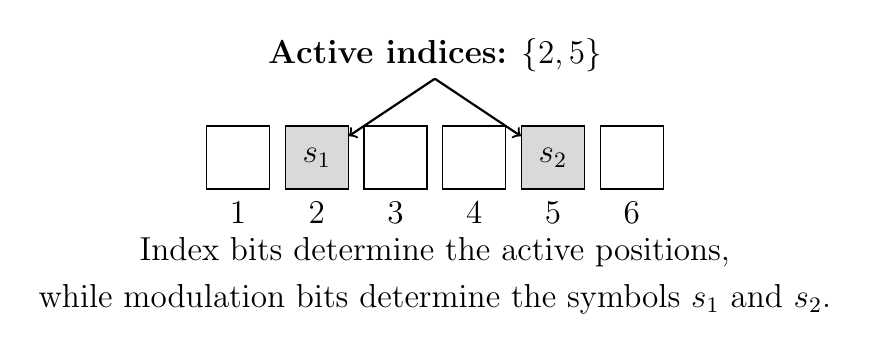
\begin{tikzpicture}[
    every node/.style={font=\small},
    active/.style={draw, fill=gray!30, minimum width=0.8cm, minimum height=0.8cm},
    inactive/.style={draw, minimum width=0.8cm, minimum height=0.8cm},
    arrow/.style={->, thick}
]

\node[align=center] at (2.5,1.3)
{\textbf{Active indices:} $\{2,5\}$};

\node[inactive] (r1) at (0,0) {};
\node[active]   (r2) at (1,0) {$s_1$};
\node[inactive] (r3) at (2,0) {};
\node[inactive] (r4) at (3,0) {};
\node[active]   (r5) at (4,0) {$s_2$};
\node[inactive] (r6) at (5,0) {};

\node at (0,-0.7) {\small 1};
\node at (1,-0.7) {\small 2};
\node at (2,-0.7) {\small 3};
\node at (3,-0.7) {\small 4};
\node at (4,-0.7) {\small 5};
\node at (5,-0.7) {\small 6};

\draw[arrow] (2.5,1.0) -- (r2);
\draw[arrow] (2.5,1.0) -- (r5);

\node[align=center] at (2.5,-1.5)
{Index bits determine the active positions,\\
while modulation bits determine the symbols $s_1$ and $s_2$.};

\end{tikzpicture}

\caption{Basic principle of index modulation using active resource elements.}
\label{fig:index_modulation_principle}
\end{figure}

As shown in Fig.~\ref{fig:index_modulation_principle}, only selected resource elements are activated in an IM-based transmission block. The receiver detects both the active indices and the transmitted constellation symbols in order to recover the original information bits.

\subsubsection{OFDM-IM Systems}

One of the most widely studied applications of Index Modulation is OFDM with Index Modulation (OFDM-IM). In conventional OFDM, all subcarriers are generally used to transmit constellation symbols. In OFDM-IM, however, only a subset of subcarriers within each subblock is activated, and the indices of these active subcarriers are used to convey additional information bits.

For an OFDM-IM subblock with \(n\) subcarriers, \(k\) active subcarriers, and \(M_{\mathrm{mod}}\)-ary modulation, the total number of transmitted bits per subblock is given by

\begin{equation}
p_{\mathrm{OFDM\text{-}IM}}
=
\left\lfloor \log_2 \binom{n}{k} \right\rfloor
+
k \log_2 M_{\mathrm{mod}}.
\end{equation}

The first term corresponds to the index bits, while the second term corresponds to the conventional modulation bits carried by the active subcarriers. Therefore, OFDM-IM can be viewed as an extension of OFDM in which subcarrier activation patterns introduce an additional information-carrying dimension.

\begin{figure}[H]
\centering

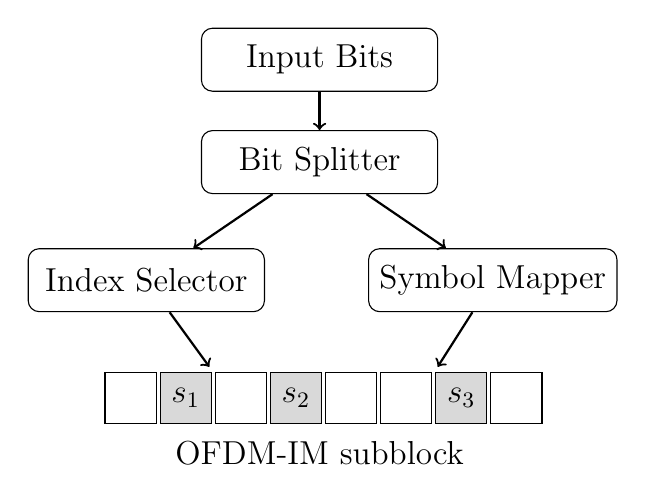
\begin{tikzpicture}[
    every node/.style={font=\small},
    block/.style={
        draw,
        rounded corners,
        minimum width=3.0cm,
        minimum height=0.8cm,
        align=center
    },
    arrow/.style={->, thick},
    active/.style={draw, fill=gray!30, minimum width=0.65cm, minimum height=0.65cm},
    inactive/.style={draw, minimum width=0.65cm, minimum height=0.65cm}
]

\node[block] (bits) at (0,0) {Input Bits};
\node[block] (split) at (0,-1.3) {Bit Splitter};
\node[block] (index) at (-2.2,-2.8) {Index Selector};
\node[block] (mapper) at (2.2,-2.8) {Symbol Mapper};

\draw[arrow] (bits) -- (split);
\draw[arrow] (split) -- (index);
\draw[arrow] (split) -- (mapper);

\node[inactive] (s1) at (-2.4,-4.3) {};
\node[active]   (s2) at (-1.7,-4.3) {$s_1$};
\node[inactive] (s3) at (-1.0,-4.3) {};
\node[active]   (s4) at (-0.3,-4.3) {$s_2$};
\node[inactive] (s5) at (0.4,-4.3) {};
\node[inactive] (s6) at (1.1,-4.3) {};
\node[active]   (s7) at (1.8,-4.3) {$s_3$};
\node[inactive] (s8) at (2.5,-4.3) {};

\node at (0,-5.0) {OFDM-IM subblock};

\draw[arrow] (index) -- (-1.4,-3.9);
\draw[arrow] (mapper) -- (1.5,-3.9);

\end{tikzpicture}

\caption{Conceptual structure of an OFDM-IM subblock.}
\label{fig:ofdm_im_subblock}
\end{figure}

The OFDM-IM concept provides a useful foundation for understanding more advanced IM-based systems. Since the present thesis focuses on OTFS-IM, the detailed mathematical design of OFDM-IM is not discussed extensively in this chapter. Instead, OFDM-IM is introduced as a representative example showing how index patterns can be exploited for information transmission.

\subsubsection{Advantages and Challenges of IM}

Index Modulation offers several attractive advantages for wireless communication systems. First, it provides an additional mechanism for conveying information without relying solely on constellation symbols. This can improve spectral efficiency or allow lower modulation orders to be used for a given transmission rate.

Second, IM offers flexibility in resource allocation. By changing the number of active resources, modulation order, and index mapping strategy, the system can be adapted to different performance requirements. For example, increasing the number of active resources may improve data rate, while reducing the number of active resources may reduce transmit energy and interference.

Third, IM can improve error performance in certain channel conditions because inactive resource elements provide additional structure that may assist detection at the receiver. The sparsity introduced by index activation can also be beneficial for receiver design, especially in systems where the channel itself has a sparse structure.

However, Index Modulation also introduces several challenges. The receiver must detect both the active indices and the transmitted symbols, which may increase detection complexity compared with conventional modulation. Furthermore, incorrect detection of active indices can lead to multiple bit errors because both index bits and symbol bits may be affected.

Another challenge is the design of efficient index mapping tables. Since the number of available activation patterns \(\binom{n}{k}\) is not always a power of two, only a subset of all possible patterns may be used in practical systems. This may lead to unused patterns and requires careful mapping design.

The main advantages and challenges of Index Modulation are summarized in Table~\ref{tab:im_advantages_challenges}.

\begin{table}[H]
\centering
\caption{Advantages and challenges of Index Modulation.}
\label{tab:im_advantages_challenges}

\small
\setlength{\tabcolsep}{6pt}
\begin{tabularx}{0.95\textwidth}{|>{\RaggedRight\arraybackslash}p{0.31\textwidth}|>{\RaggedRight\arraybackslash}X|}
\hline
\textbf{Aspect} &
\textbf{Description} \\
\hline

Additional information dimension &
Information is transmitted through both constellation symbols and active indices. \\
\hline

Flexible system design &
The number of active resources and modulation order can be adjusted according to system requirements. \\
\hline

Potential energy efficiency &
Only selected resources are active in each transmission block. \\
\hline

Detection complexity &
The receiver must jointly detect active indices and transmitted symbols. \\
\hline

Index detection errors &
Incorrect index detection may cause multiple bit errors. \\
\hline

Mapping design &
Efficient mapping is required when the number of activation patterns is not a power of two. \\
\hline

\end{tabularx}

\end{table}

In the context of this thesis, Index Modulation is considered as a promising technique to enhance OTFS transmission. The detailed OTFS-IM system model, including index mapping in the delay-Doppler domain, transmitter structure, receiver detection, and performance evaluation, will be presented in Chapter 4.


\subsection{Chapter Summary}

This chapter presented the theoretical background required for the study of OTFS and OTFS-IM systems. The fundamental characteristics of wireless communication channels were first introduced, including channel impairments, channel classification, multipath propagation, delay spread, Doppler effects, and doubly selective fading channels.

The chapter then reviewed the principles of OFDM, including its transceiver structure, advantages, and limitations in high-mobility environments. Although OFDM provides high spectral efficiency and simple frequency-domain equalization, its performance degrades significantly when severe Doppler spread destroys subcarrier orthogonality and introduces inter-carrier interference.

The delay-Doppler domain representation was also discussed as an alternative way to characterize time-varying wireless channels. This representation describes wireless propagation in terms of delay and Doppler shifts, providing a more suitable foundation for understanding OTFS modulation. Finally, the basic concept of Index Modulation was introduced, including its principle, OFDM-IM structure, advantages, and challenges.

Overall, this chapter established the necessary theoretical foundation for the following chapters. Based on these concepts, Chapter 3 will present the principles and mathematical formulation of OTFS modulation in more detail.

\newpage

\newpage

\section*{CHAPTER 3. OTFS SYSTEM DESIGN AND MODELING}
\addcontentsline{toc}{section}{CHAPTER 3. OTFS SYSTEM DESIGN AND MODELING}

% =========================================================
% Numbering for Chapter 3
% =========================================================
\setcounter{section}{3}
\setcounter{subsection}{0}
\setcounter{subsubsection}{0}
\setcounter{figure}{0}
\setcounter{table}{0}
\setcounter{equation}{0}

\renewcommand{\thefigure}{3.\arabic{figure}}
\renewcommand{\thetable}{3.\arabic{table}}
\renewcommand{\theequation}{3.\arabic{equation}}
\renewcommand{\theHfigure}{3.\arabic{figure}}
\renewcommand{\theHtable}{3.\arabic{table}}
\renewcommand{\theHequation}{3.\arabic{equation}}

% =========================================================
% Chapter Introduction
% =========================================================
This chapter develops the baseline OTFS system used as the reference model for the rest of the thesis. It describes the OTFS transceiver architecture, transmitter and receiver processing chains, delay-Doppler channel model, equivalent input-output relation, and message passing detector, following the main OTFS and iterative detection principles reported in the literature~\cite{Hadani2018OTFS,Raviteja2018OTFSMP,Raviteja2018OTFSInterference}. The objective is to establish a clear baseline before introducing index modulation in Chapter 4.

\begin{figure}[H]
    \centering
    \resizebox{0.98\linewidth}{!}{%
    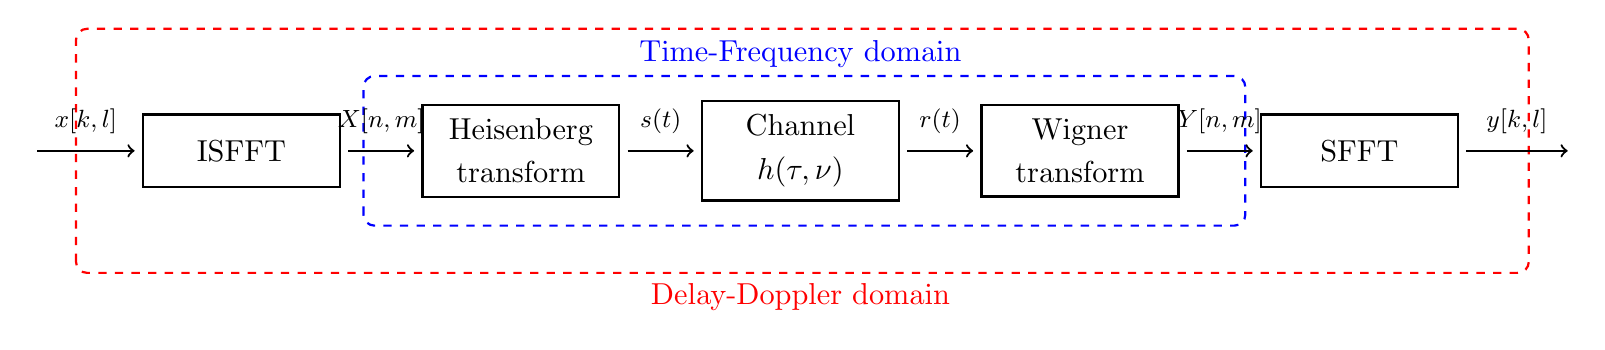
\begin{tikzpicture}[
        block/.style={
            rectangle,
            draw,
            thick,
            align=center,
            text width=2.15cm,
            minimum height=0.92cm,
            font=\footnotesize,
            inner sep=5pt,
            outer sep=0pt
        },
        arrow/.style={
            ->,
            thick,
            shorten >=3pt,
            shorten <=3pt
        }
    ]

        \node[block] (isfft) at (0,0) {ISFFT};
        \node[block] (heis) at (3.55,0) {Heisenberg\\transform};
        \node[block] (chan) at (7.10,0) {Channel\\\(h(\tau,\nu)\)};
        \node[block] (wig) at (10.65,0) {Wigner\\transform};
        \node[block] (sfft) at (14.20,0) {SFFT};

        \draw[dashed, red, thick, rounded corners]
            (-2.10,-1.55) rectangle (16.35,1.55);
        \node[red, font=\footnotesize] at (7.10,-1.86) {Delay-Doppler domain};

        \draw[dashed, blue, thick, rounded corners]
            (1.55,-0.95) rectangle (12.75,0.95);
        \node[blue, font=\footnotesize] at (7.10,1.23) {Time-Frequency domain};

        \draw[arrow] (-2.70,0) -- node[midway, above, yshift=2pt, font=\scriptsize] {\(x[k,l]\)} (isfft.west);
        \draw[arrow] (isfft.east) -- node[midway, above, yshift=2pt, font=\scriptsize] {\(X[n,m]\)} (heis.west);
        \draw[arrow] (heis.east) -- node[midway, above, yshift=2pt, font=\scriptsize] {\(s(t)\)} (chan.west);
        \draw[arrow] (chan.east) -- node[midway, above, yshift=2pt, font=\scriptsize] {\(r(t)\)} (wig.west);
        \draw[arrow] (wig.east) -- node[midway, above, yshift=2pt, font=\scriptsize] {\(Y[n,m]\)} (sfft.west);
        \draw[arrow] (sfft.east) -- node[midway, above, yshift=2pt, font=\scriptsize] {\(y[k,l]\)} (16.95,0);

    \end{tikzpicture}
    }
    \caption{Overall baseline OTFS transceiver architecture}
    \label{fig:baseline_otfs_transceiver_architecture}
\end{figure}


% =========================================================
% Chapter Sections
% =========================================================
\subsection{Design Objectives and System Assumptions}

This section defines the design objectives, system configuration, and main assumptions of the baseline OTFS system used in this thesis. The baseline system is designed as the reference model for the OTFS-IM extension in Chapter 4 and for the numerical comparison in Chapter 5. Therefore, the model must be detailed enough to represent the essential OTFS transmission mechanism, while remaining sufficiently controlled so that the effects of index modulation and pattern selection can be evaluated clearly.

\subsubsection{Design Objectives}

The first objective of the baseline OTFS system is to establish a complete end-to-end transmission chain operating through the delay-Doppler domain. Unlike OFDM, where information symbols are directly arranged in the time-frequency domain, OTFS places data symbols on a two-dimensional delay-Doppler grid before transforming them for transmission. This structure allows the channel effects caused by multipath delay and Doppler shift to be represented more explicitly in the signal model.

The second objective is to provide a fair reference for the OTFS-IM system developed later in this thesis. Since OTFS-IM changes the way information bits are mapped onto the delay-Doppler grid, its performance must be evaluated against a conventional OTFS baseline using the same frame dimensions, modulation order, channel model, noise definition, and detector assumptions. This makes it possible to determine whether the observed performance difference comes from the index-modulation structure and pattern design, rather than from inconsistent simulation settings.

The third objective is to define the receiver structure used as the foundation for later detection analysis. In this thesis, the baseline OTFS receiver uses a message passing detector. This detector is suitable for sparse delay-Doppler channel structures and provides a natural basis for the OTFS-IM receiver, where both QAM symbols and active-position patterns must be detected. Therefore, the baseline OTFS model is not only a comparison curve in the BER results, but also the starting point for the receiver design in the proposed OTFS-IM framework.

\subsubsection{Delay-Doppler Grid and Frame Structure}

The baseline OTFS frame is constructed on a two-dimensional delay-Doppler grid with \(N\) Doppler bins and \(M\) delay bins. The transmitted delay-Doppler symbol matrix is denoted as
\begin{equation}
    \mathbf{x}_{\mathrm{DD}}
    =
    [x[k,l]]
    \in \mathbb{C}^{N \times M},
\end{equation}
where \(k\) is the Doppler index and \(l\) is the delay index. The element \(x[k,l]\) represents the QAM information symbol placed at the \(k\)-th Doppler bin and the \(l\)-th delay bin.

In the baseline OTFS system, all delay-Doppler resource elements are active. Hence, each frame contains
\begin{equation}
    N_{\mathrm{RE}} = MN
\end{equation}
resource elements, and each resource element carries one QAM symbol. This is different from the OTFS-IM system introduced in Chapter 4, where only a subset of positions in each index-modulation block is active and the activation pattern itself also conveys information.

If the QAM modulation order is denoted by \(M_{\mathrm{QAM}}\), then each QAM symbol carries
\begin{equation}
    b_{\mathrm{QAM}} = \log_2(M_{\mathrm{QAM}})
\end{equation}
information bits. Therefore, the total number of information bits transmitted in one baseline OTFS frame is
\begin{equation}
    B_{\mathrm{OTFS}} = MN \log_2(M_{\mathrm{QAM}}).
\end{equation}
The corresponding spectral efficiency, measured in bits per delay-Doppler resource element, is
\begin{equation}
    \eta_{\mathrm{OTFS}}
    =
    \frac{B_{\mathrm{OTFS}}}{MN}
    =
    \log_2(M_{\mathrm{QAM}}).
\end{equation}

For the numerical simulations in this thesis, the baseline OTFS system uses 4-QAM modulation. Thus,
\begin{equation}
    M_{\mathrm{QAM}} = 4,
    \qquad
    b_{\mathrm{QAM}} = 2.
\end{equation}
The baseline spectral efficiency is therefore
\begin{equation}
    \eta_{\mathrm{OTFS}} = 2
    \quad \text{bits/resource element}.
\end{equation}

The selected OTFS grid size is
\begin{equation}
    N = 10, \qquad M = 12,
\end{equation}
which gives
\begin{equation}
    MN = 120
\end{equation}
delay-Doppler resource elements per frame. Since 4-QAM is used, the number of information bits transmitted in one baseline OTFS frame is
\begin{equation}
    B_{\mathrm{OTFS}} = 120 \times 2 = 240
    \quad \text{bits/frame}.
\end{equation}

The main simulation parameters of the baseline OTFS system are summarized in Table~\ref{tab:baseline_otfs_parameters}. This table is placed here because these parameters are repeatedly used in the transmitter design, receiver design, and performance evaluation sections.

\begin{table}[H]
    \centering
    \caption{Baseline OTFS simulation parameters}
    \label{tab:baseline_otfs_parameters}
    \begin{tabular}{c c c}
        \hline
        Parameter & Symbol & Value \\
        \hline
        Number of Doppler bins & \(N\) & 10 \\
        Number of delay bins & \(M\) & 12 \\
        Resource elements per frame & \(MN\) & 120 \\
        QAM modulation order & \(M_{\mathrm{QAM}}\) & 4-QAM \\
        Bits per QAM symbol & \(b_{\mathrm{QAM}}\) & 2 \\
        Baseline spectral efficiency & \(\eta_{\mathrm{OTFS}}\) & 2 bits/resource element \\
        Information bits per OTFS frame & \(B_{\mathrm{OTFS}}\) & 240 bits \\
        \(E_b/N_0\) range & \(E_b/N_0\) & 0:5:20 dB \\
        OTFS Monte Carlo frames & \(N_{\mathrm{fram}}\) & 1000 \\
        OFDM-LMMSE Monte Carlo frames & \(N_{\mathrm{fram,OFDM}}\) & 1000 \\
        \hline
    \end{tabular}
\end{table}

The selected grid size provides a compact simulation setting that keeps the Monte Carlo evaluation computationally feasible. This is important because the thesis later evaluates multiple OTFS-IM configurations and pattern-selection methods under the same channel and noise conditions. The same delay-Doppler frame dimensions are also used as the reference grid for OTFS-IM, so that performance differences can be interpreted in terms of modulation structure and receiver behavior rather than different frame sizes.

\subsubsection{Transceiver Assumptions}

The system considered in this thesis is a single-input single-output transmission system. This assumption keeps the focus on the modulation structure, channel effect, and receiver detection process. Although multi-antenna transmission is important for practical wireless systems, including MIMO processing would introduce additional spatial-domain operations that are outside the main scope of this work.

Perfect timing and frequency synchronization are assumed at the receiver. Under this assumption, the received OTFS frame can be demodulated without additional synchronization errors. This choice is suitable for the baseline design because synchronization impairments would introduce another source of degradation and make it more difficult to isolate the effects of OTFS modulation and OTFS-IM pattern selection.

The receiver is also assumed to have access to the channel parameters required by the detector. In other words, the detection process is evaluated under a perfect-CSI assumption. This does not imply that channel estimation is unimportant in practical OTFS systems. Rather, channel estimation is excluded so that the thesis can focus on modulation, index-pattern design, and detection reliability under controlled conditions.

\subsubsection{Channel Assumptions}

The wireless channel is modeled as a time-varying multipath Rayleigh fading channel in the delay-Doppler domain. Each propagation path is represented by a delay tap, a Doppler tap, and a complex fading coefficient. The delay tap models the propagation delay of a multipath component, while the Doppler tap represents the time variation induced by relative motion or dynamic scattering in the propagation environment.

The complex path coefficients are generated as complex Gaussian random variables with delay-dependent power scaling. As a result, the channel amplitudes follow a Rayleigh fading behavior. Additive white Gaussian noise is then added after the multipath channel. This model allows the simulation to capture the combined effects of multipath fading, delay spread, Doppler spread, and thermal noise.

In this thesis, the Doppler shifts are represented by normalized discrete Doppler taps on the OTFS grid. Therefore, the channel captures Doppler-induced time selectivity without assigning a specific physical velocity in kilometres per hour. This modeling choice is appropriate for the objective of the thesis, which is to evaluate OFDM, OTFS, and OTFS-IM under a common high-Doppler delay-Doppler fading condition, rather than to reproduce a standardized vehicular channel model.

This assumption should be interpreted carefully. The simulated channel represents the main impairment associated with high-mobility communication, namely Doppler-induced time variation. However, it is not claimed to correspond exactly to a particular vehicle speed. For this reason, the channel is described as a high-Doppler or mobility-like delay-Doppler fading channel in the simulation discussion.

\subsubsection{Fairness Criteria for Comparison}

A key requirement of the simulation framework is fairness. The OFDM, OTFS, and OTFS-IM systems are evaluated over the same \(E_b/N_0\) range and under the same channel generation mechanism. This ensures that the performance differences observed in Chapter 5 mainly arise from the modulation and detection structures, rather than from inconsistent channel or noise assumptions.

The OFDM reference used in this thesis is denoted as OFDM-LMMSE. It uses a full-frame linear minimum mean square error equalizer with channel knowledge. This makes the OFDM baseline stronger and more meaningful than a simple one-tap OFDM receiver in a time-varying channel. Therefore, any gain achieved by OTFS or OTFS-IM is compared against an OFDM receiver that already includes explicit equalization.

For the OTFS baseline, the same channel realization style and noise definition are used. The receiver uses a message passing detector, which is suitable for sparse delay-Doppler channel structures. In Chapter 4, the OTFS-IM receiver builds on this detection framework by using probability information to identify both QAM symbols and activation patterns.

Spectral efficiency is also considered when interpreting the results. Since the baseline OTFS system with 4-QAM has a spectral efficiency of \(2\) bits/resource element, OTFS-IM configurations with the same value are treated as rate-fair comparisons. Configurations with lower spectral efficiency are interpreted as reliability-oriented cases, where reduced rate is exchanged for improved BER performance. This distinction is important because OTFS-IM does not automatically outperform OTFS in every configuration; its advantage depends on the trade-off among spectral efficiency, pattern detection reliability, and symbol detection accuracy.

\subsubsection{Scope of the Baseline Model}

The baseline OTFS model is intentionally compact and controlled. It does not include channel coding, channel estimation error, synchronization offset, MIMO transmission, or standardized 5G channel profiles. These components are important in practical systems, but including all of them would make it harder to isolate the contribution of OTFS-IM activation-pattern design.

The role of the baseline model is therefore to provide a clean and consistent reference system. It defines the delay-Doppler frame, the modulation format, the channel assumptions, and the receiver detection structure used throughout the thesis. Based on this baseline, Chapter 4 introduces index modulation into the OTFS grid and studies how activation-pattern design affects index BER, symbol BER, pattern error rate, and total BER.

\subsection{OTFS Transmitter Design}

\subsubsection{Overview of the Transmitter Processing Chain}

The OTFS transmitter is designed to convert a binary information sequence into a time-domain waveform suitable for transmission over a time-varying multipath channel. The key idea is that the information symbols are first arranged in the delay-Doppler domain, rather than being transmitted directly in the time-frequency domain. This processing structure allows the transmitted frame to be associated with the delay and Doppler characteristics of the wireless channel.

The overall transmitter chain used in the baseline OTFS system is illustrated in Fig.~\ref{fig:otfs_transmitter_chain}. The input bit sequence is first mapped into QAM symbols. These symbols are then placed on the delay-Doppler grid to form the matrix \(\mathbf{x}_{\mathrm{DD}}\). After that, the inverse symplectic finite Fourier transform is applied to convert the delay-Doppler symbols into the time-frequency domain. The resulting time-frequency symbols are finally transformed into a time-domain transmit signal by the Heisenberg transform, or equivalently by its discrete implementation in the simulation.

\begin{figure}[H]
    \centering
    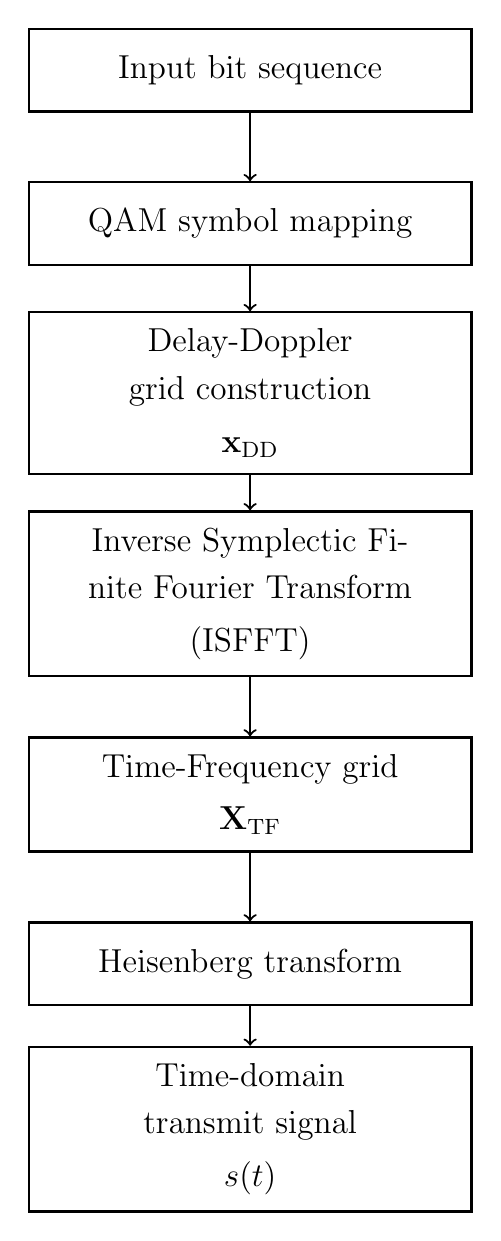
\begin{tikzpicture}[
        block/.style={
            rectangle,
            draw,
            thick,
            align=center,
            text width=5.2cm,
            minimum height=1.05cm,
            font=\small,
            inner sep=6pt
        },
        arrow/.style={
            ->,
            thick,
            shorten >=0pt,
            shorten <=0pt
        }
    ]

        \node[block] (bits) at (0,0) {Input bit sequence};
        \node[block] (qam) at (0,-1.95) {QAM symbol mapping};
        \node[block] (dd) at (0,-4.10) {Delay-Doppler grid construction\\[2pt]\(\mathbf{x}_{\mathrm{DD}}\)};
        \node[block] (isfft) at (0,-6.65) {Inverse Symplectic Finite Fourier Transform\\[2pt](ISFFT)};
        \node[block] (tf) at (0,-9.20) {Time-Frequency grid\\[2pt]\(\mathbf{X}_{\mathrm{TF}}\)};
        \node[block] (heis) at (0,-11.35) {Heisenberg transform};
        \node[block] (tx) at (0,-13.45) {Time-domain transmit signal\\[2pt]\(s(t)\)};

        \draw[arrow] (bits.south) -- (qam.north);
        \draw[arrow] (qam.south) -- (dd.north);
        \draw[arrow] (dd.south) -- (isfft.north);
        \draw[arrow] (isfft.south) -- (tf.north);
        \draw[arrow] (tf.south) -- (heis.north);
        \draw[arrow] (heis.south) -- (tx.north);

    \end{tikzpicture}
    \caption{Baseline OTFS transmitter processing chain}
    \label{fig:otfs_transmitter_chain}
\end{figure}

The transmitter can therefore be viewed as a sequence of four main operations. The first operation is bit-to-symbol mapping, where the input bits are grouped and mapped to QAM constellation points. The second operation is delay-Doppler grid construction, where the QAM symbols are arranged over the \(N \times M\) OTFS frame. The third operation is the inverse symplectic finite Fourier transform, which maps the delay-Doppler representation to the time-frequency representation. The final operation is time-domain signal generation, where the time-frequency samples are converted into the transmitted waveform.

This separation of operations is useful because each stage has a distinct role in the OTFS system. The QAM mapper determines the number of bits carried by each active resource element. The delay-Doppler grid defines the information-bearing structure of the OTFS frame. The ISFFT performs the domain transformation required by OTFS modulation, while the Heisenberg transform generates the signal that is actually transmitted through the channel. In the baseline OTFS system, all delay-Doppler grid positions are active, which makes the transmitter structure simpler than the OTFS-IM transmitter introduced in Chapter 4.

In the discrete simulation model, the transmitter follows the same conceptual chain. A random bit sequence is generated and mapped to 4-QAM symbols. The symbol vector is reshaped into an \(N \times M\) delay-Doppler matrix. The OTFS modulation stage then performs the discrete transform operations and serializes the result into a time-domain vector. This vector is used as the input to the multipath delay-Doppler channel model described in the next section.

\subsubsection{Bit-to-QAM Symbol Mapping}

The first stage of the baseline OTFS transmitter is the mapping of information bits to QAM symbols. In the OTFS notation used in this thesis, the information symbols before modulation are denoted by \(x[k,l]\), where \(k\) is the Doppler index and \(l\) is the delay index. These symbols form the delay-Doppler information grid that will later be transformed into the time-frequency domain.

For one OTFS frame, the transmitter generates a binary information sequence with
\begin{equation}
    B_{\mathrm{OTFS}} = MN\log_2(M_{\mathrm{QAM}})
\end{equation}
bits, where \(M_{\mathrm{QAM}}\) is the QAM modulation order. For the baseline setup, \(N=10\), \(M=12\), and \(M_{\mathrm{QAM}}=4\), so one OTFS frame contains
\begin{equation}
    B_{\mathrm{OTFS}} = 10 \times 12 \times \log_2(4) = 240
\end{equation}
information bits.

The input bit sequence is divided into groups of \(\log_2(M_{\mathrm{QAM}})\) bits. Each group is converted into a decimal symbol index and then mapped to one QAM constellation point. This produces a vector of \(MN\) complex-valued QAM symbols. This mapping is represented by
\begin{equation}
    \mathbf{x}
    =
    \mathcal{Q}_{M_{\mathrm{QAM}}}
    \left(
    \mathbf{b}
    \right),
\end{equation}
where \(\mathcal{Q}_{M_{\mathrm{QAM}}}(\cdot)\) denotes grouping the input bits and mapping each group to an \(M_{\mathrm{QAM}}\)-ary QAM constellation point.

After QAM mapping, the symbol vector is reshaped into the delay-Doppler grid as
\begin{equation}
    \mathbf{x}_{\mathrm{DD}}
    =
    \left[
    x[k,l]
    \right]_{N \times M}.
\end{equation}
In the code, this step is performed by
\begin{equation}
    \mathbf{x}_{\mathrm{DD}}
    =
    \mathrm{reshape}(\mathbf{x},N,M).
\end{equation}

For the baseline OTFS system, all positions on the delay-Doppler grid are active. Therefore, every element \(x[k,l]\) carries one QAM symbol. This is an important difference from the OTFS-IM transmitter introduced in Chapter 4, where only selected positions are active and the active-position pattern itself also conveys information.

With 4-QAM modulation, each delay-Doppler resource element carries two information bits. Therefore, the baseline OTFS transmitter maps the 240 input bits of one frame into 120 QAM symbols and places them over the full \(10 \times 12\) delay-Doppler grid. The resulting matrix \(\mathbf{x}_{\mathrm{DD}}\) is then used as the input to the OTFS modulation block.

\subsubsection{Delay-Doppler Grid Construction}

After QAM symbol mapping, the next stage is to arrange the modulated symbols onto the OTFS delay-Doppler grid. This grid is the information-bearing domain of OTFS. Instead of assigning symbols directly to time-frequency resource elements as in OFDM, OTFS first places the QAM symbols in the delay-Doppler domain. The subsequent OTFS modulation stages then spread these symbols over the time-frequency plane before transmission.

Let the QAM symbol vector generated by the previous stage be denoted by
\begin{equation}
    \mathbf{x}
    =
    [x_0,x_1,\ldots,x_{MN-1}]^T.
\end{equation}
This vector contains \(MN\) complex-valued QAM symbols. In the baseline OTFS transmitter, these symbols are reshaped into the delay-Doppler symbol matrix
\begin{equation}
    \mathbf{x}_{\mathrm{DD}}
    =
    [x[k,l]]
    \in \mathbb{C}^{N \times M},
\end{equation}
where \(k=0,1,\ldots,N-1\) denotes the Doppler index and \(l=0,1,\ldots,M-1\) denotes the delay index.

The mapping from the one-dimensional QAM symbol vector to the two-dimensional delay-Doppler grid can be written as
\begin{equation}
    x[k,l] = x_{k + lN},
    \qquad
    0 \leq k \leq N-1,\quad 0 \leq l \leq M-1.
\end{equation}
This indexing follows a fixed column-wise ordering when the one-dimensional symbol sequence is arranged into the \(N \times M\) delay-Doppler grid. Equivalently, the reshaping operation can be represented as
\begin{equation}
    \mathbf{x}_{\mathrm{DD}}
    =
    \mathrm{reshape}(\mathbf{x},N,M).
\end{equation}

For the baseline OTFS system, every position of the delay-Doppler grid is occupied by one QAM symbol. Therefore, the grid contains no inactive resource elements. This full-grid structure is important because it defines the conventional OTFS reference system. In Chapter 4, the OTFS-IM transmitter modifies this structure by dividing the grid into index-modulation blocks and activating only selected positions inside each block.

For the simulation configuration used in this thesis, the grid size is \(N=10\) and \(M=12\). Hence, the delay-Doppler grid contains \(120\) symbol positions. With 4-QAM modulation, the transmitter maps \(240\) input bits into \(120\) QAM symbols and places them over the full delay-Doppler grid. The resulting matrix \(\mathbf{x}_{\mathrm{DD}}\) is then used as the input to the inverse symplectic finite Fourier transform in the next stage of the OTFS modulator.

A conceptual view of the baseline delay-Doppler grid is shown in Fig.~\ref{fig:baseline_dd_grid}. Each cell represents one delay-Doppler resource element, and all cells are active in the baseline OTFS system.

\begin{figure}[H]
    \centering
    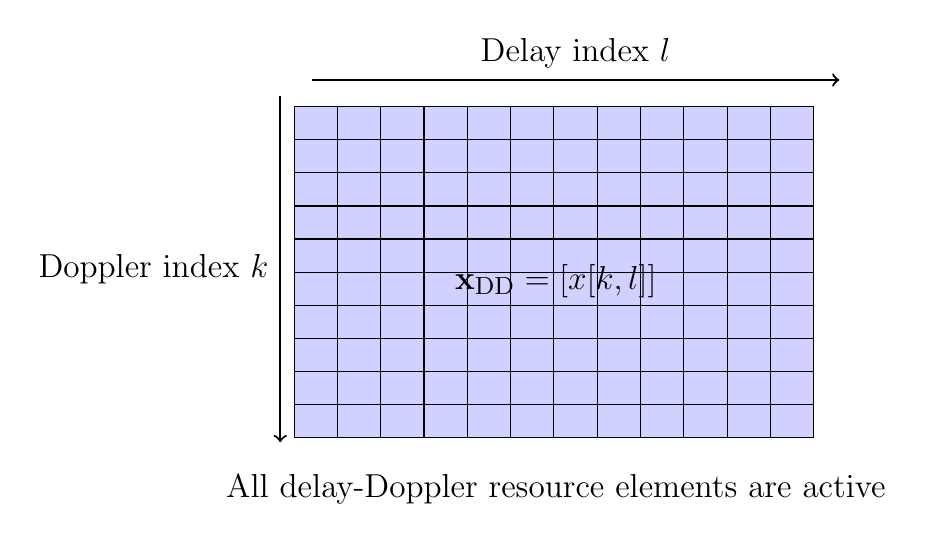
\begin{tikzpicture}[
        cell/.style={
            rectangle,
            draw,
            minimum width=0.55cm,
            minimum height=0.42cm
        },
        active/.style={
            fill=blue!18
        }
    ]

        \foreach \i in {0,...,9} {
            \foreach \j in {0,...,11} {
                \node[cell, active] at (\j*0.55,-\i*0.42) {};
            }
        }

        \draw[->, thick] (-0.45,0.35) -- (-0.45,-4.05)
            node[midway, left] {Doppler index \(k\)};
        \draw[->, thick] (-0.05,0.55) -- (6.65,0.55)
            node[midway, above] {Delay index \(l\)};

        \node at (3.05,-2.0) {\(\mathbf{x}_{\mathrm{DD}}=[x[k,l]]\)};
        \node[align=center] at (3.05,-4.65) {All delay-Doppler resource elements are active};

    \end{tikzpicture}
    \caption{Baseline OTFS delay-Doppler grid with full resource activation}
    \label{fig:baseline_dd_grid}
\end{figure}

\subsubsection{Inverse Symplectic Finite Fourier Transform}

After the QAM symbols are arranged on the delay-Doppler grid, the next step of the OTFS transmitter is to transform them into the time-frequency domain. This operation is performed by the inverse symplectic finite Fourier transform. The ISFFT is one of the core operations of OTFS modulation because it connects the information-bearing delay-Doppler representation to the time-frequency representation used for waveform generation.

Let the delay-Doppler symbol matrix be denoted by
\begin{equation}
    \mathbf{x}_{\mathrm{DD}} = [x[k,l]],
\end{equation}
where \(k=0,1,\ldots,N-1\) is the Doppler index and \(l=0,1,\ldots,M-1\) is the delay index. The ISFFT maps \(x[k,l]\) into the time-frequency symbols \(X[n,m]\), where \(n=0,1,\ldots,N-1\) denotes the time index and \(m=0,1,\ldots,M-1\) denotes the frequency index.

Using the OTFS convention adopted in this thesis, the ISFFT can be written as
\begin{equation}
    X[n,m]
    =
    \frac{1}{\sqrt{MN}}
    \sum_{k=0}^{N-1}
    \sum_{l=0}^{M-1}
    x[k,l]
    e^{j2\pi\left(\frac{nk}{N}-\frac{ml}{M}\right)}.
    \label{eq:isfft}
\end{equation}
The resulting matrix
\begin{equation}
    \mathbf{X}_{\mathrm{TF}}
    =
    [X[n,m]]
    \in \mathbb{C}^{N \times M}
\end{equation}
represents the OTFS frame in the time-frequency domain.

The structure of the ISFFT is different from a conventional two-dimensional inverse Fourier transform because the signs of the Fourier kernels are opposite along the two dimensions. This symplectic structure reflects the dual relationship between the delay-Doppler and time-frequency domains. In particular, the Doppler dimension is transformed with respect to the time index, while the delay dimension is transformed with respect to the frequency index.

For the discrete implementation used in the simulation model, the ISFFT operation is evaluated through a pair of finite Fourier transforms along the two grid dimensions:
\begin{equation}
    \mathbf{X}_{\mathrm{TF}}
    =
    \mathrm{fft}
    \left(
    \mathrm{ifft}
    \left(
    \mathbf{x}_{\mathrm{DD}}
    \right)^T
    \right)^T
    \bigg/
    \sqrt{\frac{M}{N}}.
    \label{eq:isfft_matlab}
\end{equation}
This expression is the matrix-form counterpart of the ISFFT in \eqref{eq:isfft}. The two transform directions correspond to the delay and Doppler dimensions, while the normalization factor preserves the energy scale of the OTFS frame.

The normalization factor is included to preserve the signal energy across the domain transformation. This is important for BER simulation because the noise variance is computed from the selected \(E_b/N_0\) value. If the transform scaling were inconsistent, the effective received SNR would be shifted, making the BER comparison between OFDM, OTFS, and OTFS-IM unfair.

After the ISFFT, each delay-Doppler information symbol has been spread across the time-frequency grid. This spreading property is one of the reasons OTFS is suitable for time-varying multipath channels. Instead of assigning each information symbol to a single time-frequency resource element, OTFS distributes the symbol over the frame before waveform generation. The time-frequency matrix \(\mathbf{X}_{\mathrm{TF}}\) is then passed to the Heisenberg transform to generate the time-domain transmit signal.

\subsubsection{Heisenberg Transform and Time-Domain Signal Generation}

After the ISFFT, the OTFS frame is represented by the time-frequency symbol matrix
\begin{equation}
    \mathbf{X}_{\mathrm{TF}} = [X[n,m]],
\end{equation}
where \(n=0,1,\ldots,N-1\) is the time index and \(m=0,1,\ldots,M-1\) is the frequency index. The purpose of the Heisenberg transform is to convert these time-frequency samples into a continuous-time transmit waveform.

In the general OTFS formulation, the transmitted signal can be expressed as
\begin{equation}
    s(t)
    =
    \sum_{n=0}^{N-1}
    \sum_{m=0}^{M-1}
    X[n,m]\,
    g_{\mathrm{tx}}(t-nT)
    e^{j2\pi m\Delta f(t-nT)},
    \label{eq:heisenberg_transform}
\end{equation}
where \(g_{\mathrm{tx}}(t)\) is the transmit pulse, \(T\) is the symbol duration, and \(\Delta f\) is the subcarrier spacing. This expression shows that each time-frequency sample \(X[n,m]\) modulates a time-shifted and frequency-shifted version of the transmit pulse.

The Heisenberg transform can be viewed as the waveform-generation stage of the OTFS transmitter. While the delay-Doppler grid defines where the information symbols are placed, and the ISFFT maps them into the time-frequency domain, the Heisenberg transform produces the actual signal that enters the wireless channel. Therefore, it plays a role similar to the multicarrier modulation stage in OFDM, but it operates on the time-frequency samples generated from the delay-Doppler information grid.

In the discrete model used in this thesis, the Heisenberg transform is represented after the ISFFT by applying an inverse Fourier transform along the frequency-related dimension:
\begin{equation}
    \mathbf{s}_{\mathrm{mat}}
    =
    \mathrm{ifft}
    \left(
    \mathbf{X}_{\mathrm{TF}}^T
    \right)
    \sqrt{M}.
    \label{eq:heisenberg_matlab}
\end{equation}
This matrix \(\mathbf{s}_{\mathrm{mat}}\) contains the time-domain samples associated with the time-frequency grid \(\mathbf{X}_{\mathrm{TF}}\). The scaling factor keeps the discrete waveform normalization consistent with the ISFFT stage.

The matrix \(\mathbf{s}_{\mathrm{mat}}\) contains the discrete time-domain samples before serialization. To form the transmit vector, the matrix is converted into a column vector according to
\begin{equation}
    \mathbf{s}
    =
    \mathrm{vec}
    \left(
    \mathbf{s}_{\mathrm{mat}}
    \right).
    \label{eq:tx_vector}
\end{equation}
The vectorization step preserves the sample ordering used by the OTFS frame and produces a one-dimensional transmit sequence suitable for the channel model.

The output vector \(\mathbf{s}\) is the discrete-time transmit signal used as the input to the wireless channel model. In the simulation framework, this signal is passed to the time-varying multipath channel model, where delay taps, Doppler taps, fading coefficients, and additive noise are applied. Therefore, the Heisenberg transform and serialization stage completes the baseline OTFS transmitter processing chain.

\subsubsection{Discrete Processing Summary}

The baseline OTFS transmitter can be summarized by three discrete signal-processing operations: ISFFT, discrete Heisenberg transformation, and serialization. The input is the delay-Doppler matrix \(\mathbf{x}_{\mathrm{DD}}\), obtained by arranging the QAM symbol vector according to the \(N \times M\) frame ordering described earlier. The output is the time-domain transmit vector \(\mathbf{s}\).

The complete discrete transmitter chain can therefore be summarized as
\begin{equation}
\begin{aligned}
    \mathbf{X}_{\mathrm{TF}}
    &=
    \mathrm{fft}
    \left(
    \mathrm{ifft}
    \left(
    \mathbf{x}_{\mathrm{DD}}
    \right)^T
    \right)^T
    \bigg/
    \sqrt{\frac{M}{N}},
    \\
    \mathbf{s}_{\mathrm{mat}}
    &=
    \mathrm{ifft}
    \left(
    \mathbf{X}_{\mathrm{TF}}^T
    \right)
    \sqrt{M},
    \\
    \mathbf{s}
    &=
    \mathrm{vec}
    \left(
    \mathbf{s}_{\mathrm{mat}}
    \right).
\end{aligned}
\end{equation}

This compact representation is important for the rest of the thesis because the same OTFS modulation principle is used for both the baseline OTFS system and the later OTFS-IM system. The difference between the two systems is not in the modulation transform itself, but in the construction of the delay-Doppler input matrix. In the baseline OTFS system, every delay-Doppler position carries a QAM symbol, while in OTFS-IM only selected positions are active according to an index-modulation pattern.

\subsubsection{Summary of the Baseline OTFS Transmitter}

The baseline OTFS transmitter converts a binary information sequence into a time-domain signal through a sequence of delay-Doppler and time-frequency processing stages. The input bits are first mapped to QAM symbols and arranged on the delay-Doppler grid as \(x[k,l]\). In the baseline system, all delay-Doppler resource elements are active, so every grid position carries one QAM symbol.

The delay-Doppler symbol matrix \(\mathbf{x}_{\mathrm{DD}}\) is then transformed into the time-frequency domain by the ISFFT. This produces the time-frequency matrix \(\mathbf{X}_{\mathrm{TF}}\), whose elements \(X[n,m]\) are used for waveform generation. The discrete Heisenberg transform is finally applied to obtain the time-domain transmit vector \(\mathbf{s}\).

The transmitter chain can be summarized as
\begin{equation}
    \mathbf{b}
    \rightarrow
    \mathbf{x}
    \rightarrow
    \mathbf{x}_{\mathrm{DD}}
    \xrightarrow{\mathrm{ISFFT}}
    \mathbf{X}_{\mathrm{TF}}
    \xrightarrow{\mathrm{Heisenberg}}
    \mathbf{s}.
\end{equation}

This structure highlights the main difference between OTFS and conventional OFDM. In OFDM, information symbols are directly assigned to time-frequency resource elements. In OTFS, the information symbols are first placed in the delay-Doppler domain and then spread across the time-frequency plane before transmission. This spreading allows the transmitted frame to interact with the delay-Doppler structure of the wireless channel.

The same OTFS modulation block is reused later for the OTFS-IM transmitter. The key difference is the construction of the delay-Doppler input matrix. In the baseline OTFS system, every grid position is active. In OTFS-IM, only selected positions are active, and their indices carry additional information bits. Therefore, the baseline transmitter developed in this section provides the foundation for the OTFS-IM design in Chapter 4.

After the time-domain signal \(\mathbf{s}\) is generated, it is passed through the time-varying multipath channel. The design of this channel model and its delay-Doppler characteristics are discussed in the next section.


\subsection{Channel Model Design}

This section describes the wireless channel model used in the baseline OTFS simulation. The purpose of the channel model is to represent a time-varying multipath propagation environment with both delay and Doppler effects. The same channel generation mechanism is used for OFDM-LMMSE, baseline OTFS, and OTFS-IM so that the performance comparison in Chapter 5 remains consistent.

\subsubsection{Time-Varying Multipath Channel Overview}

In OTFS theory, a time-varying wireless channel can be represented in the delay-Doppler domain by a finite number of propagation paths. Each path is characterized by a delay, a Doppler shift, and a complex channel coefficient. This representation is suitable for OTFS because the transmitted information symbols are first arranged in the delay-Doppler domain before being transformed for transmission.

In the simulation model used in this thesis, the continuous delay-Doppler channel is represented by discrete channel taps. The channel is described by
\begin{equation}
    \{h_i,l_i,\nu_i\}_{i=1}^{P},
\end{equation}
where \(P\) is the number of channel paths, \(h_i\) is the complex fading coefficient of the \(i\)-th path, \(l_i\) is the discrete delay tap, and \(\nu_i\) is the discrete Doppler tap. In this model, \(\nu_i\) denotes a Doppler-tap index on the OTFS grid rather than a physical Doppler frequency in hertz. The Doppler tap is therefore represented as a normalized integer index on the OTFS Doppler grid.

A conceptual representation of the channel model is shown in Fig.~\ref{fig:discrete_multipath_channel}. The transmitted signal is passed through several delayed, Doppler-shifted, and faded propagation paths. The path contributions are then summed and complex additive white Gaussian noise is added.

\begin{figure}[H]
    \centering
    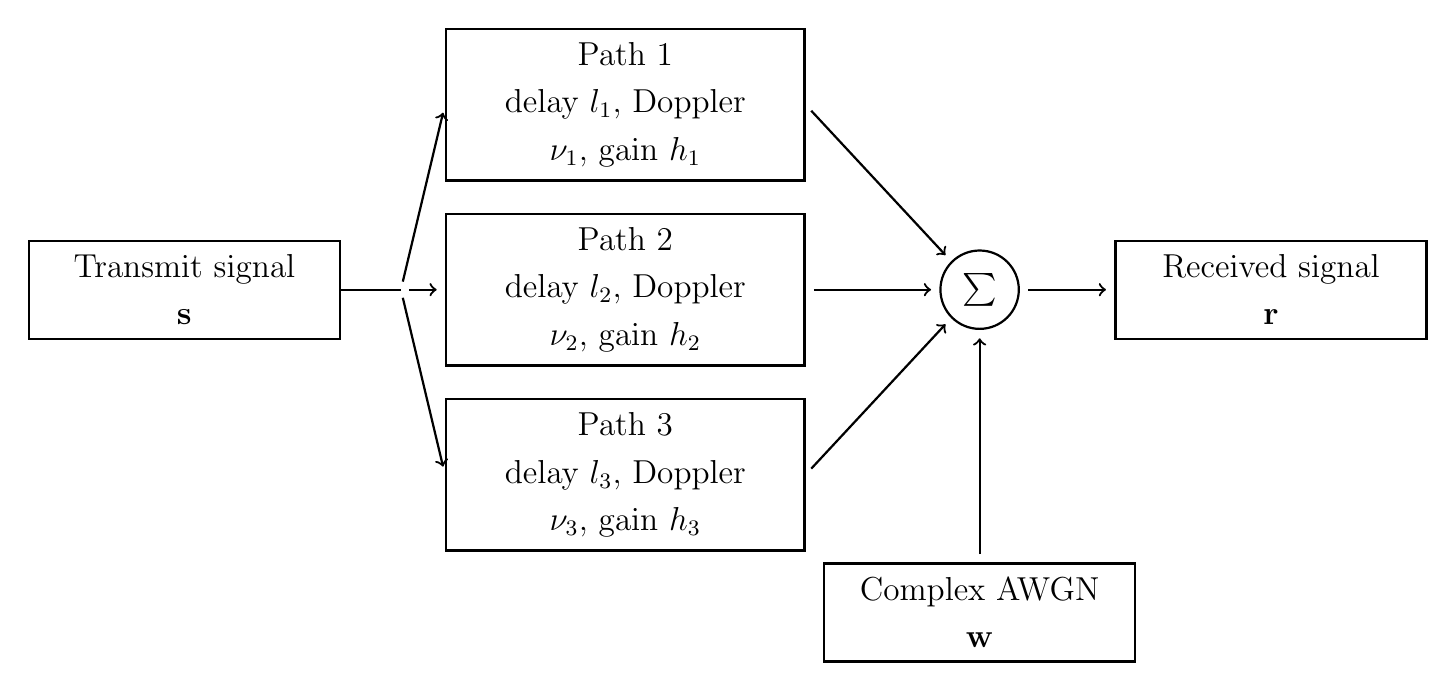
\begin{tikzpicture}[
        block/.style={
            rectangle,
            draw,
            thick,
            align=center,
            text width=3.6cm,
            minimum height=0.9cm,
            font=\small,
            inner sep=5pt
        },
        pathblock/.style={
            rectangle,
            draw,
            thick,
            align=center,
            text width=4.2cm,
            minimum height=1.05cm,
            font=\small,
            inner sep=5pt
        },
        sum/.style={
            circle,
            draw,
            thick,
            minimum size=0.8cm,
            font=\small
        },
        arrow/.style={
            ->,
            thick,
            shorten >=3pt,
            shorten <=3pt
        }
    ]

        \node[block] (input) at (0,0) {Transmit signal\\\(\mathbf{s}\)};

        \coordinate (split) at (2.75,0);

        \node[pathblock] (p1) at (5.6,2.35) {Path 1\\delay \(l_1\), Doppler \(\nu_1\), gain \(h_1\)};
        \node[pathblock] (p2) at (5.6,0) {Path 2\\delay \(l_2\), Doppler \(\nu_2\), gain \(h_2\)};
        \node[pathblock] (p3) at (5.6,-2.35) {Path 3\\delay \(l_3\), Doppler \(\nu_3\), gain \(h_3\)};

        \node[sum] (sum) at (10.1,0) {\(\sum\)};
        \node[block] (noise) at (10.1,-4.1) {Complex AWGN\\\(\mathbf{w}\)};
        \node[block] (output) at (13.8,0) {Received signal\\\(\mathbf{r}\)};

        \draw[thick] (input.east) -- (split);
        \draw[arrow] (split) -- (p1.west);
        \draw[arrow] (split) -- (p2.west);
        \draw[arrow] (split) -- (p3.west);

        \draw[arrow] (p1.east) -- (sum.north west);
        \draw[arrow] (p2.east) -- (sum.west);
        \draw[arrow] (p3.east) -- (sum.south west);

        \draw[arrow] (noise.north) -- (sum.south);
        \draw[arrow] (sum.east) -- (output.west);

    \end{tikzpicture}
    \caption{Discrete time-varying multipath channel model}
    \label{fig:discrete_multipath_channel}
\end{figure}

\subsubsection{Delay and Doppler Tap Representation}

The channel model uses three multipath components, so
\begin{equation}
    P = 3.
\end{equation}
The delay taps are fixed as
\begin{equation}
    \mathbf{l} = [0,1,2],
\end{equation}
which means that the three paths arrive with different discrete delays. These delay taps create delay spread in the received signal.

The Doppler taps are generated randomly for each channel realization. Each Doppler tap belongs to the set
\begin{equation}
    \nu_i \in \{-4,-3,-2,-1,0,1,2,3,4,5\}.
\end{equation}

The Doppler taps introduce time variation through phase rotation across the transmitted samples. A larger absolute Doppler tap produces faster phase variation. Since the Doppler values are represented as discrete indices, the model captures Doppler-induced time selectivity without assigning a specific physical velocity in kilometres per hour.

\subsubsection{Rayleigh Fading Path Coefficients}

Each channel path is assigned a complex fading coefficient. The channel coefficients are modeled as
\begin{equation}
    h_i
    =
    \sqrt{\frac{e^{-l_i}}{2}}
    \left(
    a_i + jb_i
    \right),
    \label{eq:channel_coeff}
\end{equation}
where \(a_i\) and \(b_i\) are independent real Gaussian random variables.

Because \(h_i\) is complex Gaussian, its amplitude follows a Rayleigh fading behavior. The factor \(e^{-l_i}\) introduces a delay-dependent power profile, where paths with larger delays have lower average power. This produces a simple exponentially decaying multipath channel profile.

\subsubsection{Discrete Channel Input-Output Operation}

Let \(\mathbf{s}\) be the transmitted time-domain vector generated by the OTFS transmitter. The channel output is obtained by summing the contribution of all delayed and Doppler-shifted paths. A compact discrete representation is
\begin{equation}
    r[q]
    =
    \sum_{i=1}^{P}
    h_i
    e^{j\phi_i(q)}
    s[q-l_i]
    +
    w[q],
    \label{eq:discrete_channel}
\end{equation}
where \(q\) is the discrete time-sample index, \(l_i\) is the delay tap, \(e^{j\phi_i(q)}\) is the Doppler-induced phase rotation, and \(w[q]\) is the additive noise sample.

The Doppler phase rotation is represented through the exponential term
\begin{equation}
    \exp
    \left(
    j\frac{2\pi}{M}
    q
    \frac{\nu_i}{N}
    \right).
\end{equation}
Each path contribution is then circularly shifted according to its delay tap and weighted by its complex channel coefficient.

Before applying the channel, a cyclic-prefix-like extension is added using the maximum delay tap. After the channel and noise are applied, this prefix part is removed so that the received vector has the same length as the transmitted OTFS frame.

\subsubsection{Additive White Gaussian Noise}

After the multipath channel output is generated, complex additive white Gaussian noise is added. The noise sample is modeled as
\begin{equation}
    w[q]
    =
    \sqrt{\frac{\sigma^2}{2}}
    \left(
    n_{\mathrm{I}}[q] + jn_{\mathrm{Q}}[q]
    \right),
    \label{eq:awgn}
\end{equation}
where \(n_{\mathrm{I}}[q]\) and \(n_{\mathrm{Q}}[q]\) are independent real Gaussian random variables with zero mean and unit variance.

The noise variance \(\sigma^2\) is computed from the selected \(E_b/N_0\) value and the spectral efficiency of the corresponding transmission scheme. Therefore, OFDM-LMMSE, OTFS, and OTFS-IM are evaluated under consistent energy-per-bit conditions.

\subsubsection{Channel Parameters Used in Simulation}

The main channel parameters are summarized in Table~\ref{tab:channel_model_parameters}. These parameters are used consistently across the baseline OTFS system, the OFDM-LMMSE reference, and the OTFS-IM simulations.

\begin{table}[H]
    \centering
    \caption{Delay-Doppler channel parameters used in simulation}
    \label{tab:channel_model_parameters}
    \begin{tabular}{c c c}
        \hline
        Parameter & Symbol & Value \\
        \hline
        Number of channel paths & \(P\) & 3 \\
        Delay taps & \(\mathbf{l}\) & \([0,1,2]\) \\
        Doppler tap range & \(\nu_i\) & \(-4\) to \(5\) \\
        Fading coefficient & \(h_i\) & Complex Gaussian \\
        Fading amplitude & \(|h_i|\) & Rayleigh-type fading \\
        Delay power profile & -- & Exponential decay \(e^{-l_i}\) \\
        Noise model & \(w[q]\) & Complex AWGN \\
        CSI assumption & -- & Known channel parameters at receiver \\
        \hline
    \end{tabular}
\end{table}

\subsubsection{Channel Model Summary}

The channel model used in this thesis is a discrete delay-Doppler multipath Rayleigh fading channel with additive white Gaussian noise. It includes three propagation paths, fixed delay taps, random discrete Doppler taps, and complex Gaussian fading coefficients. This structure is consistent with the OTFS principle that channels with delay and Doppler dispersion can be represented compactly in the delay-Doppler domain.

The model is intentionally controlled rather than fully standardized. It does not assign a specific mobile velocity or use a complete 3GPP channel profile. Instead, it provides a common high-Doppler delay-Doppler fading environment for comparing OFDM-LMMSE, OTFS, and OTFS-IM under the same channel conditions.


\subsection{OTFS Receiver Design}

The receiver of the baseline OTFS system performs the inverse operation of the transmitter front-end. After the transmitted waveform passes through the time-varying multipath channel, the received time-domain signal is first converted back to the time-frequency domain and then transformed to the delay-Doppler domain. The resulting delay-Doppler symbols are not directly used for hard symbol decisions. Instead, they form the observation vector for the message passing detector described in Section 3.6.

In the simulation model, the receiver processing contains two main operations: the Wigner transform and the symplectic finite Fourier transform (SFFT). The Wigner transform converts the received time-domain samples into a time-frequency grid, while the SFFT converts the time-frequency grid back to the delay-Doppler domain.

\subsubsection{Overview of the Receiver Processing Chain}

The receiver starts from the sampled received signal \(\mathbf{r}\), which includes the effect of the doubly dispersive channel and additive noise. This signal is reshaped into a two-dimensional matrix so that the receiver can process it over the same \(M \times N\) OTFS frame structure used at the transmitter. The first transform extracts the received time-frequency symbols. The second transform maps these symbols back into the delay-Doppler domain.

\begin{figure}[H]
    \centering
    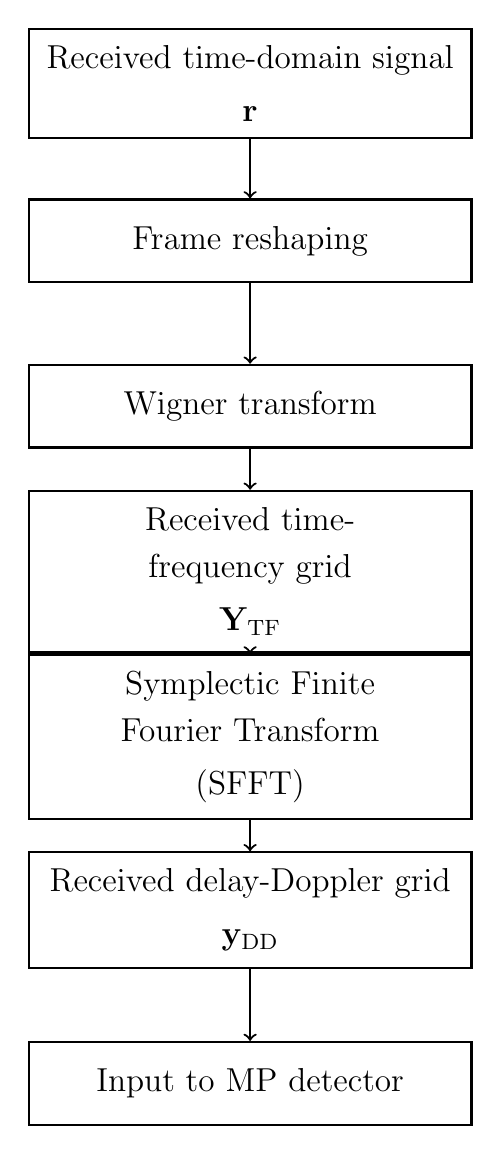
\begin{tikzpicture}[
        block/.style={
            rectangle,
            draw,
            thick,
            align=center,
            text width=5.2cm,
            minimum height=1.05cm,
            font=\small,
            inner sep=6pt
        },
        arrow/.style={
            ->,
            thick,
            shorten >=0pt,
            shorten <=0pt
        }
    ]

        \node[block] (rx) at (0,0) {Received time-domain signal\\[2pt]\(\mathbf{r}\)};
        \node[block] (reshape) at (0,-2.0) {Frame reshaping};
        \node[block] (wigner) at (0,-4.1) {Wigner transform};
        \node[block] (tf) at (0,-6.2) {Received time-frequency grid\\[2pt]\(\mathbf{Y}_{\mathrm{TF}}\)};
        \node[block] (sfft) at (0,-8.3) {Symplectic Finite Fourier Transform\\[2pt](SFFT)};
        \node[block] (dd) at (0,-10.5) {Received delay-Doppler grid\\[2pt]\(\mathbf{y}_{\mathrm{DD}}\)};
        \node[block] (detector) at (0,-12.7) {Input to MP detector};

        \draw[arrow] (rx.south) -- (reshape.north);
        \draw[arrow] (reshape.south) -- (wigner.north);
        \draw[arrow] (wigner.south) -- (tf.north);
        \draw[arrow] (tf.south) -- (sfft.north);
        \draw[arrow] (sfft.south) -- (dd.north);
        \draw[arrow] (dd.south) -- (detector.north);

    \end{tikzpicture}
    \caption{Baseline OTFS receiver processing chain}
    \label{fig:otfs_receiver_chain}
\end{figure}

Figure~\ref{fig:otfs_receiver_chain} shows that the receiver does not directly demodulate QAM symbols after the SFFT stage. This is important because the time-varying channel causes coupling among delay-Doppler symbols. Therefore, the receiver front-end only reconstructs the received delay-Doppler observation, while the actual symbol estimation is performed later by the detector.

\subsubsection{Received Signal Reshaping}

Let \(\mathbf{r}\) denote the received time-domain sample vector after the channel. This vector is reshaped into an \(M \times N\) matrix as

\begin{equation}
    \mathbf{R} = \mathrm{reshape}(\mathbf{r}, M, N).
\end{equation}

This operation restores the frame structure before applying the receiver transforms. It is the counterpart of the serialization step at the transmitter, where the time-domain transmit matrix is converted into a one-dimensional signal vector.

The reshaping operation itself does not remove channel distortion or noise. It only prepares the received samples for the Wigner transform.

\subsubsection{Wigner Transform}

The Wigner transform is used to convert the received time-domain samples into the time-frequency domain. In the discrete implementation, this operation is performed by an \(M\)-point FFT along the delay-related dimension of the reshaped received signal. The resulting time-frequency grid is denoted by \(\mathbf{Y}_{\mathrm{TF}}\).

In matrix form, the discrete Wigner stage can be represented as
\begin{equation}
    \mathbf{Y}_{\mathrm{TF}}
    =
    \left(
    \frac{1}{\sqrt{M}}\mathbf{F}_{M}\mathbf{R}
    \right)^{T},
    \label{eq:receiver_wigner_matrix}
\end{equation}
where \(\mathbf{F}_{M}\) denotes the \(M\)-point DFT matrix. The transpose follows the grid-index convention used by the transmitter-side time-frequency matrix.

The normalization factor \(\sqrt{M}\) is used to keep the signal energy consistently scaled with the transmitter implementation. After the FFT, the transpose operation arranges the matrix so that the received time-frequency samples follow the same indexing convention as the transmitted grid \(\mathbf{X}_{\mathrm{TF}}\).

Conceptually, this stage can be interpreted as the receiver counterpart of the Heisenberg transform. While the Heisenberg transform generates the time-domain waveform from the time-frequency grid, the Wigner transform extracts the time-frequency representation from the received waveform.

\subsubsection{Symplectic Finite Fourier Transform}

After obtaining the received time-frequency grid, the receiver applies the SFFT to map the signal back to the delay-Doppler domain. This is the inverse operation of the ISFFT used at the transmitter. If \(Y[n,m]\) denotes the received time-frequency sample, the corresponding delay-Doppler observation \(y[k,l]\) is obtained as

\begin{equation}
    y[k,l]
    =
    \frac{1}{\sqrt{MN}}
    \sum_{n=0}^{N-1}
    \sum_{m=0}^{M-1}
    Y[n,m]
    e^{-j2\pi\left(\frac{nk}{N}-\frac{ml}{M}\right)} .
\end{equation}

This equation is the most important receiver-side transform in the baseline OTFS model. It explains how the received signal is returned to the delay-Doppler domain, where the channel has a sparse and structured representation.

In discrete matrix processing, the SFFT combines one Fourier operation and one inverse Fourier operation along the two OTFS grid dimensions. The normalization term is selected consistently with the transmitter-side ISFFT normalization, ensuring that the overall modulation and demodulation chain has compatible energy scaling.

\subsubsection{Received Delay-Doppler Observation}

The output of the OTFS demodulator is the received delay-Doppler grid \(\mathbf{y}_{\mathrm{DD}}\). In an ideal channel without noise or Doppler-delay spreading, this grid would match the transmitted delay-Doppler symbol grid. In the simulated doubly dispersive channel, however, each received grid point may contain contributions from several transmitted symbols due to delay shifts, Doppler shifts, and complex fading coefficients.

Therefore, the received delay-Doppler grid should be understood as an observation, not as a final decision. The receiver front-end produces

\begin{equation}
    \mathbf{y}_{\mathrm{DD}} = \mathrm{SFFT}\left\{\mathbf{Y}_{\mathrm{TF}}\right\},
\end{equation}

and this observation is then passed to the message passing detector. The detector uses the channel information, delay taps, Doppler taps, and path coefficients to estimate the transmitted QAM symbols.

This separation between demodulation and detection is important in OTFS. The demodulator only changes the signal representation, while the detector resolves the interference introduced by the time-varying multipath channel.

\subsubsection{Discrete Receiver Processing Summary}

The complete receiver front-end can be summarized by the ordered sequence
\begin{equation}
    \mathbf{r}
    \xrightarrow{\text{frame reshaping}}
    \mathbf{R}
    \xrightarrow{\text{Wigner transform}}
    \mathbf{Y}_{\mathrm{TF}}
    \xrightarrow{\text{SFFT}}
    \mathbf{y}_{\mathrm{DD}} .
    \label{eq:receiver_discrete_summary}
\end{equation}
The first operation restores the received OTFS frame. The Wigner transform then extracts the time-frequency grid, and the SFFT returns the observation to the delay-Doppler domain.

This processing order is consistent with the transmitter chain. The transmitter maps delay-Doppler symbols to the time-frequency domain using the ISFFT and then generates the time-domain signal using the Heisenberg transform. The receiver reverses this order by first applying the Wigner transform and then the SFFT.

\subsubsection{Summary of the Baseline OTFS Receiver}

The baseline OTFS receiver converts the received time-domain waveform back into a delay-Doppler observation through two main operations. The Wigner transform extracts the time-frequency grid from the received samples, and the SFFT maps this grid into the delay-Doppler domain. The receiver output is not yet the estimated transmitted data, because the delay-Doppler symbols are still affected by channel-induced interference.

The overall receiver front-end can be summarized as

\begin{equation}
    \mathbf{r}
    \rightarrow
    \mathbf{R}
    \rightarrow
    \mathbf{Y}_{\mathrm{TF}}
    \rightarrow
    \mathbf{y}_{\mathrm{DD}} .
\end{equation}

The delay-Doppler observation \(\mathbf{y}_{\mathrm{DD}}\) is then used as the input to the message passing detector. This completes the receiver-side signal transformation and prepares the system for symbol estimation, which is discussed in the following sections.


\subsection{Equivalent Input-Output Model for Detection}

After OTFS demodulation, the receiver obtains the delay-Doppler observation grid \(\mathbf{y}_{\mathrm{DD}}\). This grid is not yet the final estimate of the transmitted symbols because the doubly dispersive channel introduces interference among delay-Doppler positions. At the grid level, the received delay-Doppler sample can be interpreted as a two-dimensional circular convolution between the transmitted symbols and the sparse delay-Doppler channel. A compact form of this relation is

\begin{equation}
    y[k,l]
    =
    \sum_{i=1}^{P}
    h_i
    x\!\left([\!k-\nu_i\!]_N,[\!l-l_i\!]_M\right)
    +
    w[k,l],
    \label{eq:dd_2d_convolution}
\end{equation}

where \(P\) is the number of channel paths, \(h_i\) is the complex gain of the \(i\)-th path, \(\nu_i\) and \(l_i\) denote the Doppler and delay shifts, and \([\cdot]_N\) and \([\cdot]_M\) denote circular indexing over the Doppler and delay dimensions, respectively. This expression shows that the received sample at one delay-Doppler position may contain contributions from several shifted transmitted symbols.

For detection, the two-dimensional delay-Doppler grid is rewritten into an equivalent vector input-output model. Let \(\mathbf{x}\) denote the transmitted delay-Doppler symbol vector and \(\mathbf{y}\) denote the received delay-Doppler observation vector. Both vectors have length \(MN\), where \(M\) is the number of delay bins and \(N\) is the number of Doppler bins. The equivalent input-output relation can be written as

\begin{equation}
    \mathbf{y}
    =
    \mathbf{H}_{\mathrm{DD}}\mathbf{x}
    +
    \mathbf{w},
    \label{eq:dd_input_output_model}
\end{equation}

where \(\mathbf{H}_{\mathrm{DD}}\) is the effective delay-Doppler channel matrix and \(\mathbf{w}\) is the additive noise vector after demodulation.

Equation~\eqref{eq:dd_input_output_model} is the key model used for detection. It shows that each received delay-Doppler sample is a linear combination of transmitted symbols affected by the channel. If the channel contained only a single zero-delay and zero-Doppler path, \(\mathbf{H}_{\mathrm{DD}}\) would reduce to a scaled identity-like matrix. In a time-varying multipath channel, however, delay and Doppler shifts move the transmitted symbols across the delay-Doppler grid, so the channel matrix contains structured off-diagonal components.

\subsubsection{Vector Representation of the Delay-Doppler Grid}

The transmitted delay-Doppler grid is first arranged as a two-dimensional matrix of size \(N \times M\). Equivalently, the QAM symbol vector is mapped into a fixed \(N \times M\) delay-Doppler ordering before detection.

For detection, the same grid can be represented as a vector. If \(x[k,l]\) denotes the symbol at Doppler index \(k\) and delay index \(l\), the corresponding vector element can be written as

\begin{equation}
    x_{q} = x[k,l],
    \qquad
    q = k + lN .
\end{equation}

The received delay-Doppler grid is vectorized in the same way. This vector representation is useful because the detector operates on indexed symbol positions rather than on a purely visual two-dimensional grid.

\subsubsection{Sparse Structure of the Delay-Doppler Channel}

The delay-Doppler channel matrix \(\mathbf{H}_{\mathrm{DD}}\) is sparse because the simulated channel contains only a limited number of propagation paths. Each path is characterized by a delay tap, a Doppler tap, and a complex fading coefficient. As a result, each transmitted symbol only contributes significantly to a small number of received positions.

This sparse structure is important for the message passing detector. Instead of treating every transmitted symbol as interfering with every received symbol, the detector only needs to consider the dominant connections created by the channel taps. This reduces the detection complexity compared with a full exhaustive search over all possible transmitted symbol vectors.

In the simulation, this structure is not explicitly stored as a full dense matrix. Instead, the detector uses the delay taps, Doppler taps, and channel coefficients directly. This avoids unnecessary memory usage and matches the sparse physical interpretation of the delay-Doppler channel.

\subsubsection{Role of the Equivalent Model in the Receiver}

The equivalent input-output model separates the receiver into two conceptual parts. The first part is the OTFS demodulator, which converts the received waveform into the delay-Doppler observation \(\mathbf{y}\). The second part is the detector, which estimates the transmitted symbol vector \(\mathbf{x}\) based on \(\mathbf{y}\) and the channel information.

This separation is useful because the demodulation stage only performs deterministic signal transformations, while the detection stage deals with channel-induced interference and noise. Therefore, the model in Equation~\eqref{eq:dd_input_output_model} provides the direct mathematical foundation for the message passing detector discussed in the next section.

\subsubsection{Summary of the Detection Model}

The baseline OTFS receiver can be summarized by the following delay-Doppler input-output relation:

\begin{equation}
    \mathbf{y}
    =
    \mathbf{H}_{\mathrm{DD}}\mathbf{x}
    +
    \mathbf{w}.
\end{equation}

This model shows that the received delay-Doppler vector is affected by the sparse time-varying channel and additive noise. It also explains why a dedicated detector is required after OTFS demodulation. The next section presents the message passing detector used to estimate the transmitted QAM symbols from this equivalent delay-Doppler model.


\subsection{Message Passing Detector Design}

After OTFS demodulation, the receiver obtains the delay-Doppler observation vector \(\mathbf{y}\). Because the channel is time-varying and multipath, each received delay-Doppler sample may contain contributions from several transmitted symbols. A direct exhaustive search over all possible transmitted symbol vectors would be computationally impractical. Therefore, the baseline OTFS receiver uses a message passing detector to estimate the transmitted QAM symbols from the sparse delay-Doppler input-output model.

The detector used in this thesis follows the message passing structure commonly adopted for OTFS detection over sparse delay-Doppler channels. The same detector core is later reused for OTFS-IM. In the baseline OTFS case, the detector output is used to form hard QAM symbol decisions. In the OTFS-IM case, the probability output of the same detector is further processed to detect both active positions and QAM symbols, as discussed in Chapter 4.

\subsubsection{Motivation for Message Passing Detection}

From Section 3.5, the equivalent delay-Doppler input-output relation can be written as
\begin{equation}
    \mathbf{y}
    =
    \mathbf{H}_{\mathrm{DD}}\mathbf{x}
    +
    \mathbf{w}.
\end{equation}
The matrix \(\mathbf{H}_{\mathrm{DD}}\) is sparse because the channel contains only a limited number of delay-Doppler paths. This means that each received symbol is mainly affected by a small subset of transmitted symbols, rather than by all \(MN\) transmitted symbols.

This sparse structure makes message passing suitable for OTFS detection. Instead of solving the full linear system using a dense matrix inversion, the detector iteratively exchanges probability information between received observation nodes and transmitted symbol nodes. The algorithm estimates the probability that each transmitted symbol belongs to each constellation point, and then makes a hard decision after the probabilities converge or the maximum number of iterations is reached.

\begin{figure}[H]
    \centering
    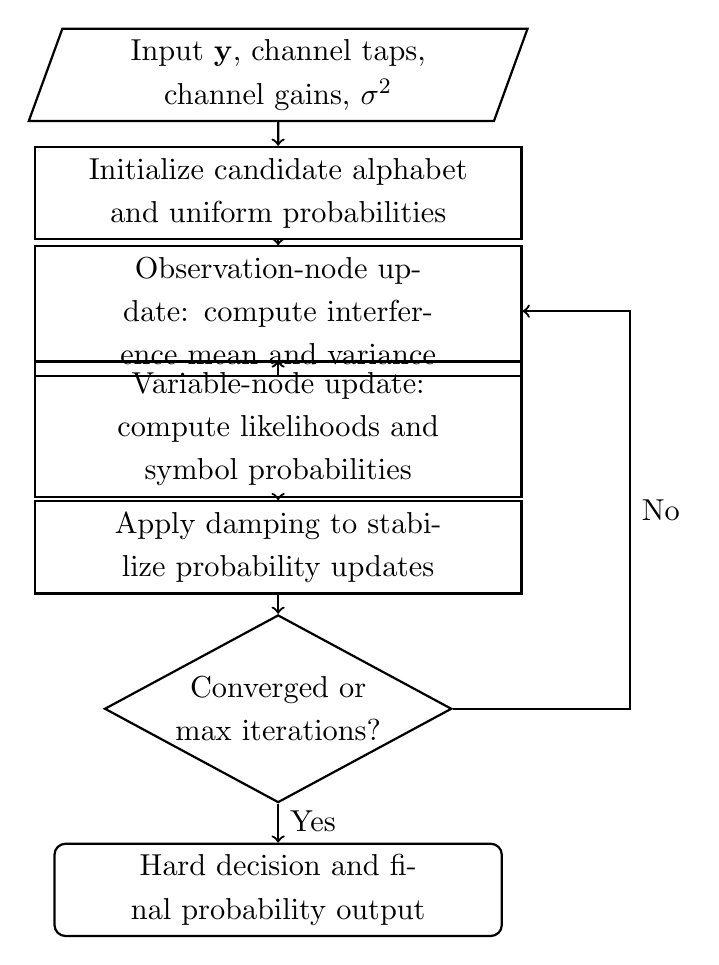
\begin{tikzpicture}[
        startstop/.style={
            rectangle,
            rounded corners,
            draw,
            thick,
            align=center,
            text width=5.4cm,
            minimum height=0.72cm,
            font=\footnotesize,
            inner sep=4pt
        },
        io/.style={
            trapezium,
            trapezium left angle=70,
            trapezium right angle=110,
            draw,
            thick,
            align=center,
            text width=5.2cm,
            minimum height=0.72cm,
            font=\footnotesize,
            inner sep=4pt
        },
        process/.style={
            rectangle,
            draw,
            thick,
            align=center,
            text width=5.9cm,
            minimum height=0.72cm,
            font=\footnotesize,
            inner sep=4pt
        },
        decision/.style={
            diamond,
            draw,
            thick,
            align=center,
            text width=2.7cm,
            aspect=1.85,
            font=\footnotesize,
            inner sep=1pt
        },
        arrow/.style={
            ->,
            thick
        }
    ]

        \node[io] (input) at (0,0) {Input \(\mathbf{y}\), channel taps, channel gains, \(\sigma^2\)};
        \node[process] (init) at (0,-1.50) {Initialize candidate alphabet and uniform probabilities};
        \node[process] (meanvar) at (0,-3.00) {Observation-node update: compute interference mean and variance};
        \node[process] (prob) at (0,-4.50) {Variable-node update: compute likelihoods and symbol probabilities};
        \node[process] (damp) at (0,-6.00) {Apply damping to stabilize probability updates};
        \node[decision] (conv) at (0,-8.05) {Converged or max iterations?};
        \node[startstop] (hard) at (0,-10.35) {Hard decision and final probability output};

        \draw[arrow] (input.south) -- (init.north);
        \draw[arrow] (init.south) -- (meanvar.north);
        \draw[arrow] (meanvar.south) -- (prob.north);
        \draw[arrow] (prob.south) -- (damp.north);
        \draw[arrow] (damp.south) -- (conv.north);
        \draw[arrow] (conv.south) -- node[right, font=\footnotesize, pos=0.45] {Yes} (hard.north);
        \draw[arrow] (conv.east) -- ++(2.25,0) |- node[pos=0.25, right, font=\footnotesize] {No} (meanvar.east);

    \end{tikzpicture}
    \caption{Operational flow of the message passing detector}
    \label{fig:mp_detector_flow}
\end{figure}

Figure~\ref{fig:mp_detector_flow} summarizes the operational flow of the detector. The algorithm starts with uniform symbol probabilities, repeatedly refines the interference statistics and symbol probabilities, and stops when the probability decisions become sufficiently reliable or when the iteration limit is reached.

\subsubsection{Sparse Factor-Graph Interpretation}

The message passing detector can be interpreted using a factor graph. In this graph, variable nodes represent transmitted symbols, while observation nodes represent received delay-Doppler samples. An edge exists between a variable node and an observation node if the corresponding transmitted symbol contributes to that received sample through one of the channel taps.

\begin{figure}[H]
    \centering
    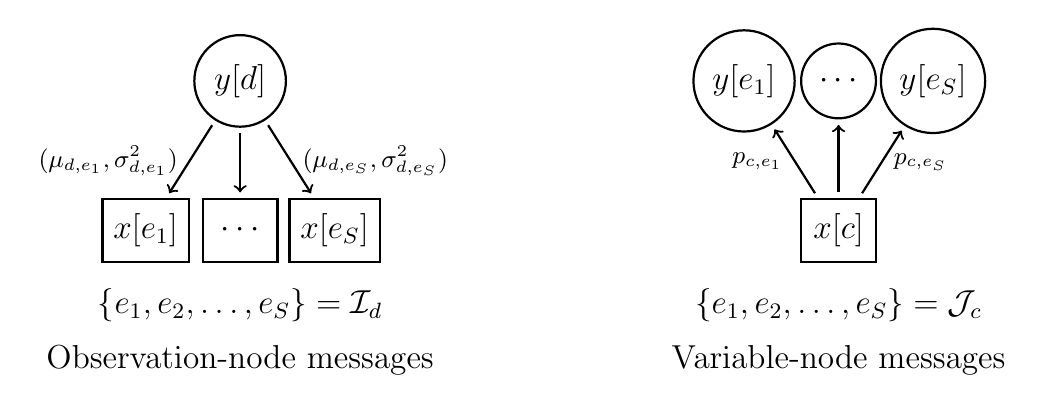
\begin{tikzpicture}[
        obsnode/.style={
            circle,
            draw,
            thick,
            align=center,
            minimum size=0.95cm,
            font=\small
        },
        varnode/.style={
            rectangle,
            draw,
            thick,
            align=center,
            minimum width=0.95cm,
            minimum height=0.8cm,
            font=\small
        },
        arrow/.style={
            ->,
            thick,
            shorten >=2pt,
            shorten <=2pt
        }
    ]

        % Observation-node messages
        \node[obsnode] (yd) at (-3.8,0.3) {\(y[d]\)};
        \node[varnode] (xe1) at (-5.0,-1.6) {\(x[e_1]\)};
        \node[varnode] (xe2) at (-3.8,-1.6) {\(\cdots\)};
        \node[varnode] (xes) at (-2.6,-1.6) {\(x[e_S]\)};

        \draw[arrow] (yd) -- node[left, font=\scriptsize, pos=0.52]
            {\((\mu_{d,e_1},\sigma^2_{d,e_1})\)} (xe1);
        \draw[arrow] (yd) -- (xe2);
        \draw[arrow] (yd) -- node[right, font=\scriptsize, pos=0.52]
            {\((\mu_{d,e_S},\sigma^2_{d,e_S})\)} (xes);

        \node[align=center, font=\small] at (-3.8,-2.55)
            {\(\{e_1,e_2,\ldots,e_S\}=\mathcal{I}_d\)};
        \node[align=center, font=\small] at (-3.8,-3.25)
            {Observation-node messages};

        % Variable-node messages
        \node[varnode] (xc) at (3.8,-1.6) {\(x[c]\)};
        \node[obsnode] (ye1) at (2.6,0.3) {\(y[e_1]\)};
        \node[obsnode] (ye2) at (3.8,0.3) {\(\cdots\)};
        \node[obsnode] (yes) at (5.0,0.3) {\(y[e_S]\)};

        \draw[arrow] (xc) -- node[left, font=\scriptsize, pos=0.50]
            {\(p_{c,e_1}\)} (ye1);
        \draw[arrow] (xc) -- (ye2);
        \draw[arrow] (xc) -- node[right, font=\scriptsize, pos=0.50]
            {\(p_{c,e_S}\)} (yes);

        \node[align=center, font=\small] at (3.8,-2.55)
            {\(\{e_1,e_2,\ldots,e_S\}=\mathcal{J}_c\)};
        \node[align=center, font=\small] at (3.8,-3.25)
            {Variable-node messages};

    \end{tikzpicture}
    \caption{Observation-node and variable-node messages in the MP detector}
    \label{fig:mp_factor_graph}
\end{figure}

Figure~\ref{fig:mp_factor_graph} illustrates the two types of messages exchanged in the MP detector. An observation node \(y[d]\) sends interference statistics, represented by the mean and variance pair \((\mu_{d,e},\sigma^2_{d,e})\), to its neighboring variable nodes. Conversely, a variable node \(x[c]\) sends probability messages \(p_{c,e}\) to the observation nodes connected to it. The neighbor sets \(\mathcal{I}_d\) and \(\mathcal{J}_c\) are determined by the delay taps, Doppler taps, and channel coefficients. Since the number of paths is small, each node is connected only to a limited number of neighboring nodes. This locality is the main reason why message passing can reduce the detection complexity.

\begin{algorithm}[H]
    \caption{Message passing detector for OTFS symbol detection}
    \label{alg:mp_detector}
    \begin{algorithmic}[1]
        \REQUIRE Received delay-Doppler vector \(\mathbf{y}\), delay taps, Doppler taps, channel coefficients, noise variance \(\sigma^2\), candidate alphabet \(\mathcal{A}_{0}\)
        \ENSURE Hard symbol estimate \(\widehat{\mathbf{x}}\) and final probability map
        \STATE Vectorize the received grid as \(\mathbf{y}=\mathrm{vec}(\mathbf{y}_{\mathrm{DD}})\)
        \STATE Initialize all symbol probabilities uniformly over \(\mathcal{A}_{0}\)
        \FOR{\(i=1\) to \(N_{\mathrm{ite}}\)}
            \STATE For each observation-symbol connection, compute the effective channel coefficient from the delay and Doppler taps
            \STATE Compute the interference mean by excluding the candidate symbol being updated
            \STATE Compute the interference variance and add the noise variance \(\sigma^2\)
            \STATE Evaluate the likelihood of every candidate symbol in \(\mathcal{A}_{0}\)
            \STATE Normalize the likelihoods to obtain updated symbol probabilities
            \STATE Apply damping between the new probabilities and the previous probabilities
            \STATE Compute the convergence rate from the maximum probability at each symbol position
            \IF{all symbol positions are reliable or the convergence rate degrades}
                \STATE Stop the iteration
            \ENDIF
        \ENDFOR
        \STATE Select the symbol with the largest final probability at each position
        \RETURN \(\widehat{\mathbf{x}}\) and the final probability map
    \end{algorithmic}
\end{algorithm}

Algorithm~\ref{alg:mp_detector} presents the computational order of the detector. The most important idea is that the detector does not decide symbols immediately after OTFS demodulation. Instead, it repeatedly estimates the interference caused by neighboring delay-Doppler symbols and uses this estimate to refine the probability of each candidate symbol.

\subsubsection{Algorithmic Complexity Interpretation}

The advantage of message passing becomes clearer when it is compared with an exhaustive detector. If all \(MN\) transmitted OTFS symbols were detected jointly, the search space would grow as \(|\mathcal{A}|^{MN}\), where \(|\mathcal{A}|\) is the constellation size. This is impossible even for moderate frame sizes. For the baseline setup in this thesis, \(MN=120\), so a full joint search over 4-QAM candidates would require \(4^{120}\) possible symbol vectors. This number is far beyond practical simulation or implementation.

The MP detector avoids this full search by using the sparse delay-Doppler channel structure. Since each received observation is connected only to a limited number of transmitted symbols, the detector updates probabilities locally rather than globally. If the number of channel paths is \(P\), the number of detector iterations is \(N_{\mathrm{ite}}\), and the candidate alphabet size is \(|\mathcal{A}_{0}|\), a useful high-level complexity description is
\begin{equation}
    \mathcal{O}
    \left(
    N_{\mathrm{ite}}
    MN
    P
    |\mathcal{A}_{0}|
    \right).
    \label{eq:mp_complexity_order}
\end{equation}
This expression is not intended to count every arithmetic operation exactly. Its purpose is to show the scaling behavior: the computational effort grows approximately linearly with the number of delay-Doppler resource elements, the number of channel paths, the number of iterations, and the number of candidate symbols.

This complexity interpretation also explains why the same detector can be reused for OTFS-IM. In OTFS-IM, the alphabet is extended by adding the inactive symbol \(0\). Therefore, the detector does not need a different factor-graph structure. It only evaluates one additional candidate state per resource element. The more difficult OTFS-IM operation is not the MP update itself, but the block-wise interpretation of the resulting probability map, which is developed in Chapter 4.

From a reporting perspective, this distinction is important. The MP detector provides a soft reliability profile over the delay-Doppler grid. The later OTFS-IM receiver then uses this reliability profile to decide which positions are active. Therefore, the detector is not only a symbol estimator; it is also the probability engine that enables index detection.

\subsubsection{Role of Damping and Stopping in the Iterative Process}

The damping factor is included because probability messages in a loopy factor graph can oscillate between iterations. In an ideal tree-structured factor graph, messages can converge in a finite number of passes. The OTFS detection graph, however, contains cycles because several transmitted symbols can affect several received observations through different delay-Doppler shifts. In this case, updating probabilities too aggressively may cause the detector to overreact to an unreliable intermediate estimate.

Damping reduces this problem by mixing the newly computed probability with the previous probability. A large damping factor gives more weight to the new likelihood information and can lead to faster convergence when the observation is reliable. A smaller damping factor makes the detector more conservative and can improve stability when the received observation is noisy or when the interference estimate is still inaccurate. The value \(\Delta=0.6\) used in the simulation therefore represents a compromise between convergence speed and numerical stability.

The convergence criterion is also important. The detector does not need to run the full number of iterations if most symbol probabilities have already become reliable. In this thesis, reliability is measured by checking whether the largest candidate probability at a symbol position exceeds a high threshold. If the maximum probability is close to one, the detector is confident about that symbol decision. If many positions remain uncertain, additional iterations may still improve the probability map.

However, more iterations do not always guarantee better BER. In a loopy message-passing detector, later iterations can sometimes reinforce an incorrect decision if the probability map becomes overconfident too early. For this reason, the stopping rule also monitors whether the convergence behavior is improving. The detector is therefore designed to stop when the probability map has become sufficiently reliable or when further iterations are unlikely to provide useful improvement.

\begin{table}[H]
\centering
\caption{Interpretation of key MP detector parameters.}
\label{tab:mp_detector_parameter_roles}
\begin{tabularx}{0.95\linewidth}{|p{3.0cm}|X|}
\hline
\textbf{Parameter} & \textbf{Role in the detector} \\
\hline
\(P\) & Number of channel paths; determines how many neighboring symbols contribute significantly to each observation. \\
\hline
\(|\mathcal{A}_{0}|\) & Number of candidate symbol states; includes QAM symbols and, for OTFS-IM reuse, the inactive zero state. \\
\hline
\(N_{\mathrm{ite}}\) & Maximum number of message-passing iterations; limits complexity and prevents endless updates. \\
\hline
\(\Delta\) & Damping factor; balances new probability information and previous messages to improve stability. \\
\hline
\(\sigma^2\) & Noise variance; affects the likelihood width and therefore the confidence of probability updates. \\
\hline
\end{tabularx}
\end{table}

Table~\ref{tab:mp_detector_parameter_roles} also shows why detector parameters must be reported together with BER results. If the number of iterations, damping factor, or noise normalization were changed, the detector output probabilities could change even under the same channel realization. Keeping these parameters fixed is therefore necessary for a fair comparison between baseline OTFS and OTFS-IM.

\subsubsection{Symbol Alphabet and Probability Initialization}

Let \(\mathcal{A}\) denote the QAM constellation alphabet. For baseline OTFS with 4-QAM, \(\mathcal{A}\) contains four constellation points. The detector estimates, for each transmitted symbol position, the probability that the symbol belongs to each element of the alphabet.

To make the detector reusable for both baseline OTFS and OTFS-IM, an extended candidate alphabet is defined as
\begin{equation}
    \mathcal{A}_{0}
    =
    \mathcal{A}
    \cup
    \{0\}.
\end{equation}
The zero symbol is included because the same detector is later used for OTFS-IM, where inactive positions correspond to zero-valued transmitted symbols. For the baseline OTFS discussion, the important point is that the detector produces symbol probabilities over the candidate alphabet. The probability output is then used either for direct hard QAM decisions in baseline OTFS or for block-wise index detection in OTFS-IM.

At the beginning of the algorithm, all symbol candidates are assigned equal probability:
\begin{equation}
    p_{c,d}^{(0)}(a_j)
    =
    \frac{1}{|\mathcal{A}_{0}|},
    \qquad
    a_j\in\mathcal{A}_{0}.
    \label{eq:mp_uniform_initialization}
\end{equation}
This initialization avoids biasing the first iteration toward any constellation point or inactive state.

\subsubsection{Observation-Node Mean and Variance Update}

Consider one received observation \(y[d]\) and one transmitted symbol \(x[c]\) connected to it. The received sample can be written as
\begin{equation}
    y[d]
    =
    H[d,c]x[c]
    +
    \sum_{e\in\mathcal{I}(d),\,e\neq c}
    H[d,e]x[e]
    +
    w[d],
    \label{eq:mp_observation_model}
\end{equation}
where \(\mathcal{I}(d)\) is the set of transmitted symbols connected to observation node \(d\). The summation term represents the interference caused by other connected symbols.

In message passing detection, this interference is approximated as a Gaussian random variable. Therefore, for each connected edge, the observation node computes the mean and variance of the interference using the current symbol probabilities. If \(p_{e,d}^{(i-1)}(a_j)\) is the probability from the previous iteration that \(x[e]=a_j\), the interference mean can be expressed as
\begin{equation}
    \mu_{d,c}^{(i)}
    =
    \sum_{e\in\mathcal{I}(d),\,e\neq c}
    \sum_{a_j\in\mathcal{A}_{0}}
    p_{e,d}^{(i-1)}(a_j)
    a_j
    H[d,e].
\end{equation}
The corresponding variance is
\begin{equation}
    \begin{aligned}
    \left(\sigma_{d,c}^{(i)}\right)^2
    &=
    \sum_{e\in\mathcal{I}(d),\,e\neq c}
    \Bigg(
    \sum_{a_j\in\mathcal{A}_{0}}
    p_{e,d}^{(i-1)}(a_j)
    |a_j|^2
    |H[d,e]|^2
    \\
    &\qquad
    -
    \left|
    \sum_{a_j\in\mathcal{A}_{0}}
    p_{e,d}^{(i-1)}(a_j)
    a_j
    H[d,e]
    \right|^2
    \Bigg)
    +
    \sigma^2.
    \end{aligned}
\end{equation}
These two quantities summarize the contribution of all interfering symbols except the candidate symbol currently being updated.

\subsubsection{Variable-Node Probability Update with Damping}

After the observation-node update, the detector updates the probability of each candidate symbol. For a candidate value \(a_j\), the likelihood is computed by comparing the received observation with the predicted contribution of \(a_j\), while treating the remaining interference as Gaussian. A compact likelihood expression is
\begin{equation}
    \xi^{(i)}(d,c,a_j)
    =
    \exp
    \left(
    -
    \frac{
    \left|
    y[d]
    -
    \mu_{d,c}^{(i)}
    -
    H[d,c]a_j
    \right|^2
    }{
    \left(\sigma_{d,c}^{(i)}\right)^2
    }
    \right).
\end{equation}
The probability of each candidate symbol is then updated using the product of the likelihoods from the connected observation nodes. This follows the standard message passing principle that a variable node combines information from its neighboring observation nodes.

For numerical stability, the probability update can be evaluated in the logarithmic domain. After the new probability is computed, damping is applied:
\begin{equation}
    p_{c,d}^{(i)}(a_j)
    =
    \Delta \widetilde{p}_{c,d}^{(i)}(a_j)
    +
    (1-\Delta)p_{c,d}^{(i-1)}(a_j),
    \label{eq:mp_damping}
\end{equation}
where \(\widetilde{p}_{c,d}^{(i)}(a_j)\) is the newly computed probability and \(\Delta\) is the damping factor. In the simulation, the damping factor is set to
\begin{equation}
    \Delta = 0.6.
\end{equation}
Damping prevents the probabilities from changing too aggressively between iterations. This helps stabilize the iterative detector, especially when the factor graph contains cycles.

\subsubsection{Hard Decision and Convergence Criterion}

At each iteration, the detector computes the final symbol probability for every transmitted position. The hard decision is obtained by selecting the candidate symbol with the largest probability:
\begin{equation}
    j^{\star}
    =
    \arg\max_{j}
    p_c(a_j).
\end{equation}
The detected symbol is then
\begin{equation}
    \widehat{x}[c] = a_{j^{\star}}.
    \label{eq:mp_hard_decision}
\end{equation}

The implementation also evaluates a convergence indicator. A symbol position is considered reliable if the maximum probability exceeds \(0.99\). The convergence rate is therefore computed as the fraction of symbol positions satisfying this condition:
\begin{equation}
    \eta^{(i)}
    =
    \frac{1}{MN}
    \sum_{c=1}^{MN}
    \mathbf{1}
    \left(
    \max_{a_j\in\mathcal{A}_{0}} p_c^{(i)}(a_j) > 0.99
    \right).
\end{equation}
If all positions become reliable, the detector stops early. Otherwise, the algorithm continues until the maximum number of iterations is reached. In the simulation, the maximum number of message passing iterations is
\begin{equation}
    N_{\mathrm{ite}} = 10.
\end{equation}

\subsubsection{Detector Input and Output Summary}

The detector takes the received delay-Doppler observation, the OTFS frame size, the QAM order, the delay and Doppler taps, the channel coefficients, and the noise variance as its main inputs. The received grid is first vectorized so that each delay-Doppler position can be treated as one variable node in the factor graph:
\begin{equation}
    \mathbf{y}_{v}
    =
    \mathrm{vec}\!\left(\mathbf{y}_{\mathrm{DD}}\right).
    \label{eq:mp_received_vectorization}
\end{equation}
The detector then initializes the probability map, iteratively updates the interference mean and variance, updates the symbol probabilities with damping, and finally returns both a hard symbol estimate and a final probability map. The hard estimate is denoted by \(\widehat{\mathbf{x}}\), while the final probability map is denoted by \(\mathbf{P}_{\mathrm{fin}}\).

For the baseline OTFS system, \(\widehat{\mathbf{x}}\) is used to recover the QAM symbols and compute the BER. For the OTFS-IM system in Chapter 4, \(\mathbf{P}_{\mathrm{fin}}\) becomes especially important because it provides the probability that each position is active or inactive. The OTFS-IM receiver then uses these probabilities to perform block-wise pattern detection. Therefore, the detector described in this section is a common receiver component shared by both the baseline OTFS and OTFS-IM systems.

\subsubsection{Summary of the Detector Design}

The message passing detector exploits the sparse structure of the delay-Doppler channel. Instead of solving the full detection problem by exhaustive search, it iteratively exchanges probability information between received observation nodes and transmitted symbol nodes. The observation-node update computes the mean and variance of the interference, while the variable-node update refines the probability of each candidate symbol.

In the baseline OTFS receiver, the detector produces hard QAM symbol decisions used for BER evaluation. In the later OTFS-IM receiver, the same probability output is reused to detect active-position patterns and QAM symbols jointly at the block level. This makes the MP detector a central component of the simulation framework and provides the receiver foundation for the OTFS-IM design developed in Chapter 4.


\subsection{OTFS Simulation Flow}

The previous sections have described the baseline OTFS system from the transmitter, channel, receiver, input-output model, and detector perspectives. This section connects these individual processing blocks into the end-to-end simulation flow used for BER evaluation. The purpose is not to introduce a new theoretical model, but to clarify how the baseline OTFS chain is executed in MATLAB before it is used as a reference system in the performance evaluation chapter.

In the simulation framework, the baseline OTFS system is evaluated through an end-to-end Monte Carlo loop. For each value of \(E_b/N_0\), the simulator generates random information bits, maps them into QAM symbols, places the symbols on the delay-Doppler grid, applies OTFS modulation, passes the transmitted signal through the delay-Doppler multipath channel, performs OTFS demodulation, detects the transmitted symbols using the MP detector, and finally computes the BER by comparing the detected bits with the transmitted bits.

\begin{figure}[H]
    \centering
    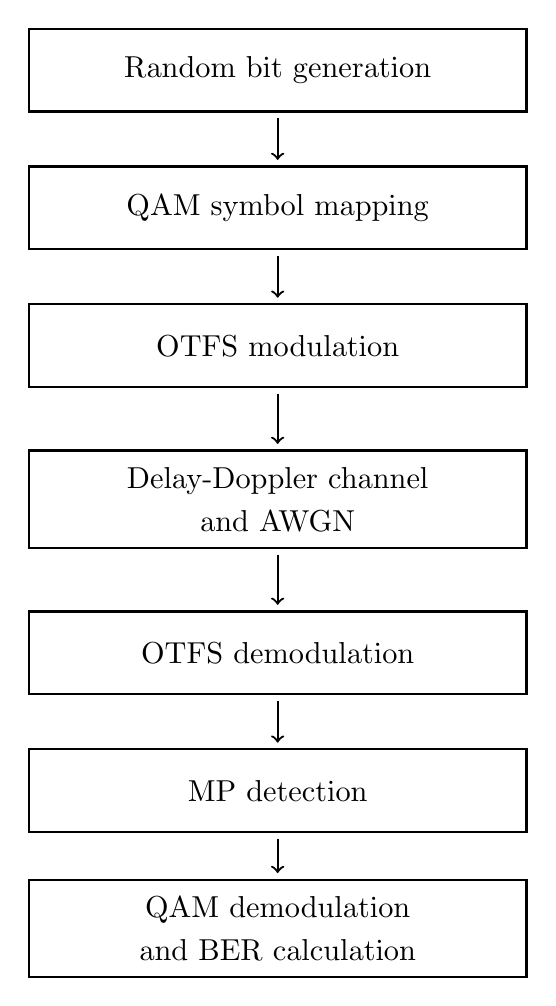
\begin{tikzpicture}[
        block/.style={
            rectangle,
            draw,
            thick,
            align=center,
            text width=5.9cm,
            minimum height=1.05cm,
            font=\footnotesize,
            inner sep=6pt
        },
        arrow/.style={
            ->,
            thick,
            shorten >=2pt,
            shorten <=2pt
        }
    ]

        \node[block] (bits) at (0,0) {Random bit generation};
        \node[block] (qam) at (0,-1.75) {QAM symbol mapping};
        \node[block] (mod) at (0,-3.50) {OTFS modulation};
        \node[block] (chan) at (0,-5.45) {Delay-Doppler channel\\and AWGN};
        \node[block] (demod) at (0,-7.40) {OTFS demodulation};
        \node[block] (mp) at (0,-9.15) {MP detection};
        \node[block] (ber) at (0,-10.90) {QAM demodulation and BER calculation};

        \draw[arrow] (bits.south) -- (qam.north);
        \draw[arrow] (qam.south) -- (mod.north);
        \draw[arrow] (mod.south) -- (chan.north);
        \draw[arrow] (chan.south) -- (demod.north);
        \draw[arrow] (demod.south) -- (mp.north);
        \draw[arrow] (mp.south) -- (ber.north);

    \end{tikzpicture}
    \caption{Baseline OTFS simulation flow used for BER evaluation}
    \label{fig:baseline_otfs_simulation_flow}
\end{figure}

Figure~\ref{fig:baseline_otfs_simulation_flow} summarizes the simulation flow. The first stage creates an equiprobable binary information sequence
\begin{equation}
    \mathbf{b}
    \in
    \{0,1\}^{N_{\mathrm{bits}}},
    \qquad
    \Pr(b_i=0)=\Pr(b_i=1)=\frac{1}{2}.
    \label{eq:baseline_random_bits}
\end{equation}
The generated bits are then grouped according to the QAM order and mapped to complex QAM symbols. For the baseline OTFS case, all delay-Doppler positions carry QAM symbols, because no index modulation is applied at this stage.

The mapped QAM symbols are reshaped into the \(N\times M\) delay-Doppler grid and processed by the OTFS transmitter described in Section 3.2. The output is a time-domain transmit vector. A channel realization is then generated by specifying the number of paths, delay taps, Doppler taps, and complex channel coefficients. The transmitted signal is passed through this time-varying multipath channel and corrupted by AWGN.

At the receiver, OTFS demodulation transforms the received time-domain signal back to the delay-Doppler observation grid. The MP detector then estimates the transmitted symbols from this observation using the sparse delay-Doppler channel structure. The estimated QAM symbols are demodulated back into bits, and the BER is computed as
\begin{equation}
    \mathrm{BER}
    =
    \frac{N_{\mathrm{err}}}{N_{\mathrm{bits}}},
\end{equation}
where \(N_{\mathrm{err}}\) is the number of incorrectly detected bits and \(N_{\mathrm{bits}}\) is the total number of transmitted bits over the simulated frames.

The baseline OTFS simulation also supports adaptive stopping in the Monte Carlo loop. If adaptive simulation is enabled, the number of frames at a given \(E_b/N_0\) point can stop early after a minimum number of frames and a target number of bit errors have been reached. This keeps the simulation practical while still collecting enough errors for BER estimation. If adaptive simulation is not enabled, the simulator uses the fixed number of frames specified in the configuration.

The baseline OTFS simulation outputs include the accumulated bit errors, the number of frames used at each SNR point, and the resulting BER vector. These outputs are later combined with the OFDM, OTFS-IM, and pattern-selection results in the main experiment runner. Therefore, the baseline OTFS flow provides the reference BER curve against which the proposed OTFS-IM schemes are evaluated in Chapter 5.


\subsection{Design Discussion and Chapter Summary}

This chapter has developed the baseline OTFS system used as the foundation for the later OTFS-IM design. The main design idea is to represent information symbols in the delay-Doppler domain, transform them to the time-frequency domain for transmission, and recover them through an OTFS receiver followed by message passing detection. This structure is suitable for time-varying multipath channels because the dominant propagation effects can be represented through a limited number of delay and Doppler taps.

The baseline system is intentionally kept as a conventional OTFS chain without index modulation. This is important for two reasons. First, it provides a clean reference that shows the performance of OTFS modulation and MP detection under the same delay-Doppler channel model used later in the thesis. Second, it allows the contribution of OTFS-IM to be evaluated separately. If index modulation were introduced too early, it would be difficult to distinguish between the benefit of the OTFS waveform itself and the effect of activating only selected positions within each IM block.

From a transmitter perspective, the baseline system maps QAM symbols directly onto the full delay-Doppler grid. The ISFFT and Heisenberg transform then produce the transmit signal. From a channel perspective, the simulation uses a discrete delay-Doppler multipath model with delay taps, Doppler taps, complex Rayleigh fading coefficients, and AWGN. From a receiver perspective, the received signal is transformed back to the delay-Doppler domain and detected using the MP detector. These blocks form a complete baseline chain that can be simulated repeatedly over different \(E_b/N_0\) values to obtain BER performance.

The use of the MP detector is a key part of the baseline receiver. A direct exhaustive search over all possible transmitted symbol vectors would be computationally expensive, especially as the frame size increases. The sparse delay-Doppler channel structure makes message passing more suitable because each received observation is connected to only a limited number of transmitted symbols. The detector therefore provides both hard symbol estimates and probability outputs. In the baseline OTFS system, the hard estimates are sufficient for BER calculation. In the OTFS-IM system developed in the next chapter, the probability outputs become more important because they support active-position and pattern detection.

The main limitation of the baseline OTFS design is that every delay-Doppler position carries a conventional modulation symbol. As a result, the baseline system does not exploit the index of active positions as an additional information-bearing dimension. It also does not provide a mechanism to study how activation-pattern design affects reliability. These limitations motivate the transition to OTFS with Index Modulation, where information is carried jointly by QAM symbols and the selected active positions inside each block.

In summary, this chapter has established the baseline OTFS transceiver, the delay-Doppler channel model, the equivalent input-output relation, the MP detector, and the MATLAB simulation flow. These components provide the reference system for the rest of the thesis. The next chapter extends this baseline by introducing OTFS-IM, block-wise active-position mapping, pattern selection, and probability-based index detection.


\newpage

\section*{CHAPTER 4. OTFS WITH INDEX MODULATION DESIGN}
\addcontentsline{toc}{section}{CHAPTER 4. OTFS WITH INDEX MODULATION DESIGN}

% =========================================================
% Numbering for Chapter 4
% =========================================================
\setcounter{section}{4}
\setcounter{subsection}{0}
\setcounter{subsubsection}{0}
\setcounter{figure}{0}
\setcounter{table}{0}
\setcounter{equation}{0}

\renewcommand{\thefigure}{4.\arabic{figure}}
\renewcommand{\thetable}{4.\arabic{table}}
\renewcommand{\theequation}{4.\arabic{equation}}
\renewcommand{\theHfigure}{4.\arabic{figure}}
\renewcommand{\theHtable}{4.\arabic{table}}
\renewcommand{\theHequation}{4.\arabic{equation}}

% =========================================================
% Chapter Introduction
% =========================================================
This chapter extends the baseline OTFS system by introducing Index Modulation in the delay-Doppler domain. The focus is on the OTFS-IM block structure, activation-pattern mapping, spectral-efficiency trade-off, transmitter and receiver design, and the OHD-based pattern-selection methods used for the simulation study in Chapter 5. The design is motivated by prior work on OTFS-IM and efficient OTFS-IM detection~\cite{Liang2020OTFSIM,Wu2024OTFSIMDetector,Qian2022BlockWiseOTFSIM,Qian2023ReceiverOTFSIM}.

% =========================================================
% Chapter Sections
% =========================================================
\subsection{OTFS-IM Design Objectives and Architecture}

This section introduces the role of OTFS-IM in the proposed system design. It clarifies why index modulation is applied in the delay-Doppler domain and how the resulting architecture extends the baseline OTFS model.

\subsubsection{Motivation and Design Objectives}

The baseline OTFS system developed in Chapter 3 places QAM symbols on all available delay-Doppler resource elements. This structure is suitable for time-varying multipath channels because the information symbols are represented in a domain where delay and Doppler effects can be described more naturally. However, the baseline OTFS transmitter uses only the symbol values themselves to convey information. The positions of the delay-Doppler resource elements are fixed and do not carry additional bits.

Index Modulation introduces a different way of using the same resource grid. Instead of activating every resource element, only a selected subset of positions is activated inside each transmission block. The activation pattern itself represents part of the transmitted information, while the active positions still carry conventional modulation symbols. In OFDM-IM, this idea is applied to frequency-domain subcarriers. In OTFS-IM, the same principle is transferred to the delay-Doppler domain, where the active delay-Doppler positions become information-bearing indices.

The motivation for combining OTFS and IM is therefore twofold. First, OTFS provides a modulation framework suitable for high-Doppler and high-mobility channels. Second, IM provides an additional information-bearing dimension through activation patterns. This combination is particularly relevant when low-order modulation is used, because the loss caused by deactivating some positions can be compensated by the additional index bits. In the present thesis, 4-QAM is used for both the baseline OTFS and OTFS-IM systems, making the IM structure meaningful from a spectral-efficiency and reliability perspective.

The main design objective of the OTFS-IM system in this thesis is to evaluate how activation-pattern design affects performance under the same delay-Doppler channel model used for the baseline OTFS system. The goal is not merely to add inactive elements to the OTFS grid, but to construct a controlled OTFS-IM framework in which index bits, QAM symbol bits, and pattern-selection rules can be evaluated separately. For this reason, the later simulation results do not report only total BER. They also separate index BER, symbol BER, and pattern error rate, because these quantities explain whether the performance is limited by QAM symbol detection or by incorrect activation-pattern detection.

Another important objective is fairness. The OTFS-IM system is compared with the baseline OTFS system using the same delay-Doppler frame size, modulation order, channel-generation method, noise definition, and detector foundation. When an OTFS-IM configuration has the same spectral efficiency as the baseline OTFS system, its BER curve can be interpreted as a rate-fair comparison. When the spectral efficiency is lower, the result is interpreted as a reliability-oriented trade-off rather than a direct throughput advantage. This distinction is important because OTFS-IM does not automatically improve BER in every configuration; its benefit depends on the number of active positions, the selected pattern table, and the reliability of the receiver.

\subsubsection{Overall OTFS-IM Transceiver Architecture}

The overall OTFS-IM transceiver can be understood as an extension of the baseline OTFS chain. The OTFS modulation and demodulation blocks remain the same as in Chapter 3. The key difference appears before OTFS modulation and after delay-Doppler-domain detection. At the transmitter, an OTFS-IM mapper converts the input bit stream into two parts: index bits and QAM symbol bits. The index bits select an activation pattern from a predefined pattern table, while the QAM symbol bits are mapped to constellation symbols placed only on the active positions.

The resulting delay-Doppler grid contains both nonzero QAM symbols and zero-valued inactive elements. This is the most fundamental structural difference between OTFS and OTFS-IM. In conventional OTFS, every delay-Doppler position carries a modulation symbol. In OTFS-IM, the zero positions are intentional and meaningful: their locations help define the selected activation pattern. Consequently, the receiver must recover not only the values of the active QAM symbols but also the pattern of active and inactive positions.

After the OTFS-IM mapper constructs the delay-Doppler grid, the remaining transmitter operations follow the baseline OTFS modulation process. The grid is transformed to the time-frequency domain by the ISFFT operation and then converted to a time-domain transmit signal by the Heisenberg transform, or equivalently by the discrete implementation used in the simulation. The signal then passes through the same time-varying delay-Doppler channel model introduced in Chapter 3.

At the receiver, the signal is demodulated back to the delay-Doppler domain. The MP detector provides probability information for each resource element. In the baseline OTFS receiver, this probability information is mainly used to make hard QAM symbol decisions. In OTFS-IM, it has a more central role because the receiver must determine whether each position is active or inactive. The receiver therefore uses the MP output probabilities to perform block-wise pattern detection and QAM symbol detection.

At the discrete processing level, the input bits are first mapped into a vectorized delay-Doppler frame, where inactive positions are kept at zero and active positions contain scaled QAM symbols. The vector is reshaped into the delay-Doppler grid and passed through the common OTFS modulation block. After channel propagation and demodulation, the MP detector produces symbol probabilities. These probabilities are then processed block by block to choose the most likely activation pattern and the most likely QAM symbols.

\begin{figure}[H]
    \centering
    \resizebox{0.98\linewidth}{!}{
    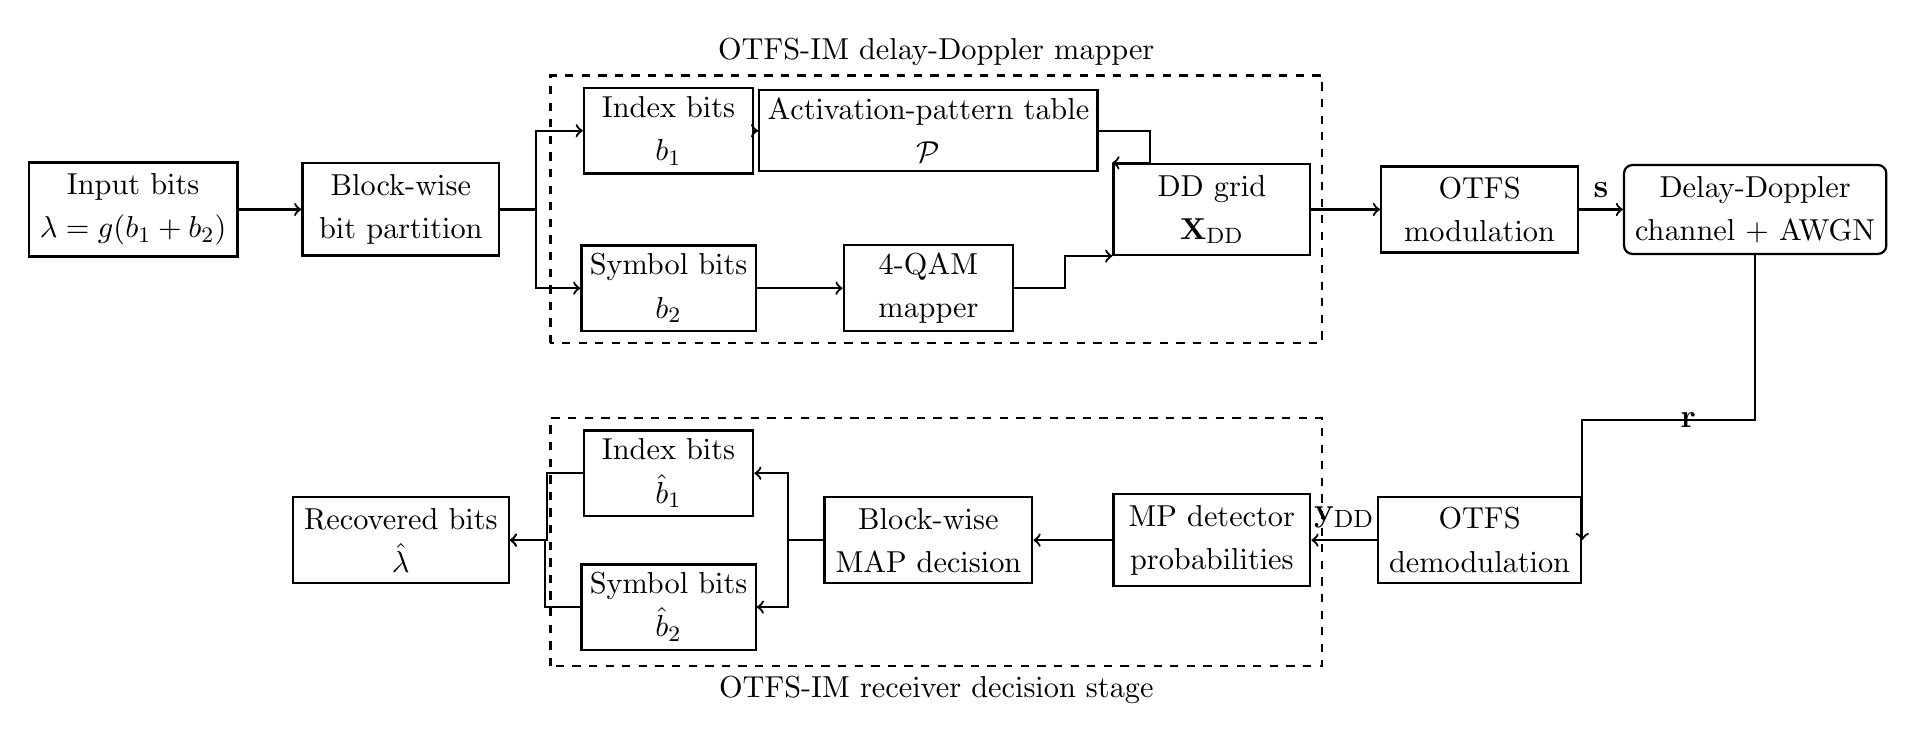
\begin{tikzpicture}[
        block/.style={
            rectangle,
            draw,
            thick,
            align=center,
            minimum width=2.5cm,
            minimum height=0.9cm,
            font=\footnotesize,
            inner sep=4pt
        },
        smallblock/.style={
            rectangle,
            draw,
            thick,
            align=center,
            minimum width=2.15cm,
            minimum height=0.75cm,
            font=\footnotesize,
            inner sep=3pt
        },
        channel/.style={
            rectangle,
            draw,
            thick,
            rounded corners=3pt,
            align=center,
            minimum width=2.6cm,
            minimum height=0.95cm,
            font=\footnotesize,
            inner sep=4pt
        },
        arrow/.style={->, thick}
    ]

        % Transmitter path
        \node[block] (inbits) at (0,0) {Input bits\\\(\lambda=g(b_1+b_2)\)};
        \node[block] (split) at (3.4,0) {Block-wise\\bit partition};
        \node[smallblock] (idx) at (6.8,1.0) {Index bits\\\(b_1\)};
        \node[smallblock] (sym) at (6.8,-1.0) {Symbol bits\\\(b_2\)};
        \node[smallblock] (map) at (10.1,1.0) {Activation-pattern table\\\(\mathcal{P}\)};
        \node[smallblock] (qam) at (10.1,-1.0) {4-QAM\\mapper};
        \node[block] (ddgrid) at (13.7,0) {DD grid\\\(\mathbf{X}_{\mathrm{DD}}\)};
        \node[block] (mod) at (17.1,0) {OTFS\\modulation};
        \node[channel] (chan) at (20.6,0) {Delay-Doppler\\channel + AWGN};

        % Receiver path
        \node[block] (demod) at (17.1,-4.2) {OTFS\\demodulation};
        \node[block] (mp) at (13.7,-4.2) {MP detector\\probabilities};
        \node[block] (mapdet) at (10.1,-4.2) {Block-wise\\MAP decision};
        \node[smallblock] (idxrx) at (6.8,-3.35) {Index bits\\\(\hat{b}_1\)};
        \node[smallblock] (symrx) at (6.8,-5.05) {Symbol bits\\\(\hat{b}_2\)};
        \node[block] (outbits) at (3.4,-4.2) {Recovered bits\\\(\hat{\lambda}\)};

        % Transmitter arrows
        \draw[arrow] (inbits.east) -- (split.west);
        \draw[arrow] (split.east) -- ++(0.45,0) |- (idx.west);
        \draw[arrow] (split.east) -- ++(0.45,0) |- (sym.west);
        \draw[arrow] (idx.east) -- (map.west);
        \draw[arrow] (sym.east) -- (qam.west);
        \draw[arrow] (map.east) -- ++(0.65,0) |- (ddgrid.north west);
        \draw[arrow] (qam.east) -- ++(0.65,0) |- (ddgrid.south west);
        \draw[arrow] (ddgrid.east) -- (mod.west);
        \draw[arrow] (mod.east) -- node[above] {\(\mathbf{s}\)} (chan.west);

        % Receiver arrows
        \draw[arrow] (chan.south) -- ++(0,-2.1) -| node[pos=0.25, right] {\(\mathbf{r}\)} (demod.east);
        \draw[arrow] (demod.west) -- node[above] {\(\mathbf{y}_{\mathrm{DD}}\)} (mp.east);
        \draw[arrow] (mp.west) -- (mapdet.east);
        \draw[arrow] (mapdet.west) -- ++(-0.45,0) |- (idxrx.east);
        \draw[arrow] (mapdet.west) -- ++(-0.45,0) |- (symrx.east);
        \draw[arrow] (idxrx.west) -- ++(-0.45,0) |- (outbits.east);
        \draw[arrow] (symrx.west) -- ++(-0.45,0) |- (outbits.east);

        \draw[dashed, thick] (5.3,-1.7) rectangle (15.1,1.7);
        \node[font=\footnotesize] at (10.2,2.0) {OTFS-IM delay-Doppler mapper};
        \draw[dashed, thick] (5.3,-5.8) rectangle (15.1,-2.65);
        \node[font=\footnotesize] at (10.2,-6.1) {OTFS-IM receiver decision stage};

    \end{tikzpicture}
    }
    \caption{Overall architecture of the implemented OTFS-IM transceiver}
    \label{fig:otfs_im_transceiver_architecture}
\end{figure}

\subsubsection{Design Scope and Relation to the Baseline OTFS System}

The OTFS-IM design in this chapter is built deliberately on top of the baseline OTFS system. The baseline system already defines the delay-Doppler grid, the modulation and demodulation operations, the channel model, and the MP detector. Chapter 4 therefore focuses only on the components that are new to OTFS-IM: block-wise mapping, activation-pattern tables, pattern selection, and block-wise receiver decisions.

This separation avoids unnecessary repetition. The ISFFT, Heisenberg transform, Wigner transform, SFFT, and delay-Doppler input-output model have already been developed in Chapter 3. In this chapter, these blocks are treated as established processing stages. The emphasis is instead placed on how the delay-Doppler input grid is constructed differently and how the receiver interprets the probability output of the detector differently.

The system considered in this thesis is an uncoded OTFS-IM system with perfect channel-state information at the receiver. Channel coding, channel estimation, synchronization errors, and standardized vehicular channel profiles are not included in the Chapter 4 design. These assumptions are consistent with the baseline model in Chapter 3 and are chosen to isolate the effect of index modulation and activation-pattern selection. Adding more practical impairments would make it harder to determine whether the observed performance difference comes from OTFS-IM itself or from another system component.

The design scope also differs from some OTFS-IM studies that focus mainly on new detector architectures such as MMSE-based or vector-wise message passing detectors. In this thesis, the receiver uses the existing MP detector as a probability engine and adds a block-wise MAP decision stage for OTFS-IM. This choice keeps the receiver structure close to the baseline OTFS system while still allowing the thesis to evaluate the reliability of index detection. The main contribution is therefore not a completely new OTFS detector, but a controlled OTFS-IM simulation framework with deterministic activation-pattern selection and detailed error-component analysis.

This design direction leads naturally to the rest of the chapter. Section 4.2 defines the IM block and spectral-efficiency calculation. Section 4.3 introduces the activation-pattern table. Section 4.4 describes the OTFS-IM transmitter. Section 4.5 presents the receiver and block-wise MAP detection process. Section 4.6 then develops the OHD and Balanced-OHD pattern-selection methods used to construct reliable activation-pattern tables.


\subsection{Index Modulation Block and Spectral Efficiency}

This section defines the OTFS-IM block structure used in the thesis and relates the mathematical parameters to the simulation model. Unlike Chapter 2, where IM was introduced as a general principle, this section focuses on how index modulation is embedded into the \(N \times M\) delay-Doppler grid of the implemented OTFS-IM system.

\subsubsection{Delay-Doppler IM Block Structure}

In the baseline OTFS system, all \(NM\) delay-Doppler resource elements are occupied by QAM symbols. In OTFS-IM, the same delay-Doppler frame is divided into smaller index-modulation blocks. Each block contains \(n\) delay-Doppler positions, of which only \(k\) positions are active. The remaining \(n-k\) positions are set to zero and are interpreted as inactive positions.

Let \(N\) denote the number of Doppler bins and \(M\) denote the number of delay bins. The total number of delay-Doppler resource elements in one OTFS frame is
\begin{equation}
    N_{\mathrm{total}} = NM .
\end{equation}
The OTFS-IM block size \(n\) is chosen such that it divides \(NM\), so that the frame can be partitioned into an integer number of IM blocks. The number of IM blocks per OTFS frame is therefore
\begin{equation}
    g = \frac{NM}{n}.
    \label{eq:otfs_im_num_blocks}
\end{equation}
The block partitioning is applied to the vectorized delay-Doppler grid. The transmit vector \(\mathbf{x}_{\mathrm{vec}}\) has length \(NM\). For the \(i\)-th IM block, the positions from \((i-1)n+1\) to \(in\) form one local activation block. The active positions inside this block are determined by the selected activation pattern, while all inactive positions remain zero.

This block-wise construction is important for two reasons. First, it defines how the input bit sequence is mapped to the delay-Doppler grid. Second, it limits the receiver search to a small block rather than the entire OTFS frame. Without this block structure, detecting the active-position pattern over all \(NM\) resource elements would be computationally impractical.

\subsubsection{Bit Partitioning and Activation Patterns}

Each OTFS-IM block carries information in two parts. The first part is represented by the activation pattern, and the second part is represented by QAM symbols transmitted on the active positions. For a block with \(n\) available positions and \(k\) active positions, the number of possible constant-weight activation patterns is \(\binom{n}{k}\). Since binary mapping requires a power-of-two number of labels, the number of index bits per block is
\begin{equation}
    b_1 =
    \left\lfloor
    \log_2 \binom{n}{k}
    \right\rfloor .
    \label{eq:otfs_im_index_bits}
\end{equation}
Only \(2^{b_1}\) patterns are selected and stored in the activation-pattern table, denoted by \(\mathcal{P}\). This table will be discussed in more detail in Section 4.3.

The second part of each block consists of QAM symbol bits. Since only \(k\) positions are active and each active position carries one \(M_{\mathrm{mod}}\)-ary QAM symbol, the number of QAM symbol bits per IM block is
\begin{equation}
    b_2 = k\log_2(M_{\mathrm{mod}}).
    \label{eq:otfs_im_symbol_bits}
\end{equation}
In this thesis, \(M_{\mathrm{mod}}=4\), so each active resource element carries two QAM bits.

Therefore, the total number of information bits per OTFS-IM block is
\begin{equation}
    b_{\mathrm{block}} = b_1 + b_2.
    \label{eq:otfs_im_bits_per_block}
\end{equation}
For one full OTFS-IM frame, the total number of transmitted bits is
\begin{equation}
    \lambda = g(b_1+b_2).
    \label{eq:otfs_im_total_bits}
\end{equation}
For each OTFS-IM frame, a binary vector of length \(\lambda\) is generated. The receiver reconstructs a vector of the same length after block-wise pattern and symbol detection.

Table~\ref{tab:otfs_im_parameters} summarizes the main OTFS-IM block parameters used in the simulation. This table is useful because Chapter 5 changes \((n,k)\) to compare different spectral-efficiency and reliability trade-offs.

\begin{table}[H]
\centering
\caption{Main OTFS-IM block parameters used in the simulation.}
\label{tab:otfs_im_parameters}
\begin{tabularx}{0.95\linewidth}{|c|c|X|}
\hline
\textbf{Symbol} & \textbf{Simulation parameter} & \textbf{Meaning} \\
\hline
\(N\) & Doppler-bin count & Number of Doppler bins in one OTFS frame. \\
\hline
\(M\) & Delay-bin count & Number of delay bins in one OTFS frame. \\
\hline
\(NM\) & Total DD resources & Total number of delay-Doppler resource elements. \\
\hline
\(n\) & IM block length & Number of resource elements in one IM block. \\
\hline
\(k\) & Active positions per block & Number of active resource elements in one IM block. \\
\hline
\(g\) & Number of IM blocks & Number of IM blocks per OTFS frame. \\
\hline
\(b_1\) & Index-bit count & Number of index bits per IM block. \\
\hline
\(b_2\) & Symbol-bit count & Number of QAM symbol bits per IM block. \\
\hline
\(\lambda\) & Frame bit length & Total number of transmitted bits per OTFS-IM frame. \\
\hline
\end{tabularx}
\end{table}

\subsubsection{Spectral Efficiency and Power Normalization}

The spectral efficiency of the baseline OTFS system is straightforward because every delay-Doppler resource element carries one QAM symbol. With \(M_{\mathrm{mod}}\)-ary QAM, the baseline OTFS spectral efficiency is
\begin{equation}
    \eta_{\mathrm{OTFS}} = \log_2(M_{\mathrm{mod}}).
    \label{eq:otfs_baseline_se}
\end{equation}
For 4-QAM, \(\eta_{\mathrm{OTFS}} = 2\) bits per delay-Doppler resource element.

For OTFS-IM, the spectral efficiency is determined by the number of transmitted bits per frame divided by the number of delay-Doppler resource elements:
\begin{equation}
    \eta_{\mathrm{IM}}
    =
    \frac{\lambda}{NM}
    =
    \frac{g(b_1+b_2)}{NM}.
    \label{eq:otfs_im_se_frame}
\end{equation}
Using \(g = NM/n\), this can also be written as
\begin{equation}
    \eta_{\mathrm{IM}}
    =
    \frac{b_1+b_2}{n}
    =
    \frac{
    \left\lfloor \log_2 \binom{n}{k} \right\rfloor
    +
    k\log_2(M_{\mathrm{mod}})
    }{n}.
    \label{eq:otfs_im_se_block}
\end{equation}
This expression is the spectral-efficiency value used to compare different OTFS-IM configurations.

Power normalization is also required because only \(k\) out of \(n\) positions are active in each IM block. If the active QAM symbols were transmitted without scaling, the average block energy would decrease simply because some positions are set to zero. To keep the energy comparison controlled, the active symbols are scaled by
\begin{equation}
    \alpha = \sqrt{\frac{n}{k}}.
    \label{eq:otfs_im_alpha}
\end{equation}
In the transmitter, the QAM symbols on active positions are multiplied by \(\alpha\). At the receiver, the demodulated delay-Doppler grid is divided by \(\alpha\), and the noise variance used by the detector is adjusted by \(\alpha^2\).

The normalization does not remove the detection difficulty of OTFS-IM. The receiver still has to distinguish active and inactive positions under noise and channel interference. Rather, the purpose of \(\alpha\) is to prevent the BER comparison from being dominated by a trivial transmit-energy mismatch between OTFS and OTFS-IM.

\subsubsection{Rate-Fair and Reliability-Oriented Configurations}

The choice of \(n\) and \(k\) determines the operating point of the OTFS-IM system. A configuration is considered rate-fair with the baseline OTFS system when
\begin{equation}
    \eta_{\mathrm{IM}} = \eta_{\mathrm{OTFS}}.
\end{equation}
Under this condition, BER curves can be compared directly because both systems transmit the same number of bits per delay-Doppler resource element.

For example, with 4-QAM and \((n,k)=(4,3)\),
\begin{equation}
    b_1 = \left\lfloor \log_2 \binom{4}{3} \right\rfloor = 2,
    \qquad
    b_2 = 3\log_2(4)=6,
\end{equation}
so that
\begin{equation}
    \eta_{\mathrm{IM}} = \frac{2+6}{4}=2
    \ \text{bits/resource element}.
\end{equation}
This is equal to the baseline OTFS spectral efficiency with 4-QAM.

Another useful equal-rate example is \((n,k)=(5,4)\). In this case,
\begin{equation}
    b_1 = \left\lfloor \log_2 \binom{5}{4} \right\rfloor = 2,
    \qquad
    b_2 = 4\log_2(4)=8,
\end{equation}
and therefore
\begin{equation}
    \eta_{\mathrm{IM}} = \frac{2+8}{5}=2
    \ \text{bits/resource element}.
\end{equation}
This configuration is also consistent with the common IM design guideline that, for low-order modulation, the number of active positions should be a large fraction of the block size when spectral efficiency is the priority.

In contrast, configurations such as \((n,k)=(4,2)\) have lower spectral efficiency:
\begin{equation}
    b_1 = \left\lfloor \log_2 \binom{4}{2} \right\rfloor = 2,
    \qquad
    b_2 = 2\log_2(4)=4,
\end{equation}
which gives
\begin{equation}
    \eta_{\mathrm{IM}} = \frac{2+4}{4}=1.5
    \ \text{bits/resource element}.
\end{equation}
Such a configuration should not be interpreted as a direct rate-fair BER comparison against baseline OTFS. Instead, it represents a reliability-oriented operating point where the system sacrifices spectral efficiency in exchange for a potentially easier detection problem.

Table~\ref{tab:otfs_im_config_examples} lists representative OTFS-IM configurations used or considered in the simulation study. The table also indicates how the corresponding results should be interpreted.

\begin{table}[H]
\centering
\caption{Representative OTFS-IM configurations and interpretation.}
\label{tab:otfs_im_config_examples}
\begin{tabular}{|c|c|c|c|c|}
\hline
\(\boldsymbol{n}\) & \(\boldsymbol{k}\) & \(\boldsymbol{b_1}\) & \(\boldsymbol{\eta_{\mathrm{IM}}}\) & \textbf{Interpretation} \\
\hline
4 & 2 & 2 & 1.50 & Reliability-oriented lower-rate case \\
\hline
4 & 3 & 2 & 2.00 & Rate-fair comparison with 4-QAM OTFS \\
\hline
5 & 4 & 2 & 2.00 & Rate-fair comparison with high active ratio \\
\hline
6 & 4 & 3 & 1.83 & Supplementary BER-SE trade-off case \\
\hline
6 & 5 & 2 & 2.00 & Rate-fair high-active-ratio validation \\
\hline
\end{tabular}
\end{table}

The selected configurations therefore serve different purposes. Rate-fair configurations are used to compare OTFS and OTFS-IM under the same spectral efficiency. Lower-rate configurations are useful for studying whether reducing the number of active positions improves the reliability of pattern and symbol detection. This distinction is carried into Chapter 5, where BER, index BER, symbol BER, and pattern error rate are interpreted together rather than relying on total BER alone.


\subsection{Activation Pattern Table Design}

After the OTFS-IM block parameters have been defined, the next design step is to determine how the index bits are converted into active delay-Doppler positions. This section describes the activation-pattern table used by the transmitter and receiver. The purpose is not only to list possible patterns, but also to explain why the pattern table has a direct influence on index detection reliability.

\subsubsection{Constant-Weight Pattern Table}

In each OTFS-IM block, exactly \(k\) out of \(n\) delay-Doppler positions are active. Therefore, every valid activation pattern has the same Hamming weight \(k\). The complete set of possible activation patterns is generated by choosing \(k\) positions from \(n\) available positions:
\begin{equation}
    \mathcal{A}_{\mathrm{all}}
    =
    \left\{
    \mathbf{a} \in \{0,1\}^{n}
    :
    \sum_{i=1}^{n} a_i = k
    \right\}.
    \label{eq:all_constant_weight_patterns}
\end{equation}
The number of candidate patterns is \(\binom{n}{k}\). Each candidate can be stored either as a set of active positions or as a binary vector. For example, when \(n=4\) and \(k=3\), a pattern row \([1,2,4]\) means that the first, second, and fourth positions in the local IM block are active, while the third position is inactive.

For distance evaluation, the position-index representation is converted into a binary vector representation. If the active positions are \([1,2,4]\), the corresponding binary pattern is
\begin{equation}
    \mathbf{a} = [1,1,0,1].
\end{equation}
This binary representation is useful because the difference between two activation patterns can be measured directly by their Hamming distance.

Although \(\binom{n}{k}\) patterns may be available, not all of them are necessarily used. The number of index bits per block is
\begin{equation}
    b_1 =
    \left\lfloor
    \log_2 \binom{n}{k}
    \right\rfloor ,
\end{equation}
so only \(2^{b_1}\) patterns can be assigned to binary input labels. The selected pattern table is denoted by
\begin{equation}
    \mathcal{P}
    =
    \left\{
    \mathbf{p}_0, \mathbf{p}_1, \ldots, \mathbf{p}_{2^{b_1}-1}
    \right\},
    \label{eq:selected_pattern_table}
\end{equation}
This table is shared by the transmitter and receiver. The transmitter uses it to decide which delay-Doppler positions are active, while the receiver uses the same table as the set of candidate patterns in the block-wise detection process.

\subsubsection{Index-to-Pattern Mapping}

In each IM block, the first \(b_1\) bits are interpreted as index bits. These bits are converted into a decimal index and then mapped to one row of the selected table \(\mathcal{P}\). The binary index is first obtained as
\begin{equation}
    q =
    \mathrm{bin2dec}
    \left(
    \mathbf{b}_{\mathrm{idx}}
    \right),
    \qquad
    q \in \{0,1,\ldots,2^{b_1}-1\}.
    \label{eq:index_binary_decimal}
\end{equation}
The simulation then applies Gray indexing before selecting the pattern row:
\begin{equation}
    m = q \oplus \left\lfloor \frac{q}{2} \right\rfloor ,
    \label{eq:gray_index_mapping}
\end{equation}
where \(\oplus\) denotes bitwise exclusive-or. The active positions for the current block are then read from
\begin{equation}
    \mathbf{p}_m = \mathcal{P}[m].
\end{equation}

For the \(i\)-th IM block, the local active positions \(\mathbf{p}_m\) are shifted to the corresponding positions in the vectorized delay-Doppler frame. The QAM symbols are inserted only at these active locations, while the other positions in the same block remain zero. Therefore, the transmitted block carries information through both the selected pattern and the QAM symbols placed on the active positions.

At the receiver, the same pattern table is used in the reverse direction. The detector evaluates every candidate row of \(\mathcal{P}\) and selects the pattern that gives the largest likelihood score. After the most likely Gray index is found, it is converted back to the original binary index bits. This ensures that the transmitter and receiver use a consistent mapping between index bits and activation patterns.

The use of a fixed pattern table is important for reproducibility. If the transmitter and receiver used different pattern ordering, the active positions might still be detected correctly but the recovered index bits would be wrong. Therefore, the pattern table must be treated as part of the system design rather than as a temporary implementation detail.

\subsubsection{Pattern-Distance Interpretation and Selection Need}

The reliability of index detection depends strongly on how distinguishable the selected activation patterns are. Two patterns that differ in only a small number of positions are more likely to be confused after channel distortion, noise, and imperfect probability estimation. This effect is measured by the Hamming distance between two binary patterns:
\begin{equation}
    d_{\mathrm{H}}(\mathbf{p}_i,\mathbf{p}_j)
    =
    \sum_{\ell=1}^{n}
    \left|
    p_i(\ell) - p_j(\ell)
    \right| .
    \label{eq:pattern_hamming_distance}
\end{equation}
For constant-weight patterns, the Hamming distance counts how many local block positions change their active or inactive status between two candidate patterns. A larger Hamming distance generally means that the receiver must make more activation-position mistakes before one pattern is confused with another.

The minimum pairwise Hamming distance of a selected pattern table is defined as
\begin{equation}
    d_{\min}
    =
    \min_{i \ne j}
    d_{\mathrm{H}}(\mathbf{p}_i,\mathbf{p}_j).
    \label{eq:pattern_min_distance}
\end{equation}
This metric is useful because the worst-separated pair of patterns often dominates the pattern error behavior. If two patterns in the table are too similar, a small detection error in one delay-Doppler position can cause an incorrect index decision.

However, maximizing only the number of possible patterns is not always the best design choice. Since only \(2^{b_1}\) patterns are used, the system has an opportunity to select a subset with better distance properties. This is the motivation for the OHD-based pattern selection methods discussed later in Section 4.6. In the present section, the important point is that \(\mathcal{P}\) is not merely a lookup table for implementation convenience. It determines the geometric separation among index labels and therefore affects index BER, pattern error rate, and total OTFS-IM BER.

In the simulation results of Chapter 5, this effect is evaluated by comparing different pattern-selection methods under the same \((n,k)\), modulation order, and channel setting. The total BER alone is not sufficient to explain the role of the activation table, so index BER and pattern error rate are also reported. These additional metrics reveal whether performance changes come from symbol detection errors or from incorrect activation-pattern decisions.


\subsection{OTFS-IM Transmitter Design}

This section describes how the OTFS-IM transmitter constructs the delay-Doppler input grid used by the common OTFS modulation block. Compared with the baseline OTFS transmitter in Chapter 3, the new operation is the block-wise mapping from input bits to activation patterns and active QAM symbols. After the OTFS-IM grid is formed, the ISFFT and Heisenberg transform are reused without structural modification.

\subsubsection{Overview of the OTFS-IM Transmitter Processing Chain}

The transmitter starts from a binary vector of length \(\lambda\), where
\begin{equation}
    \lambda = g(b_1+b_2).
\end{equation}
This vector is processed block by block. In each block, the first \(b_1\) bits select the activation pattern, while the following \(b_2\) bits are mapped to QAM symbols. Only the selected active positions are filled with QAM symbols; all other positions remain zero.

Figure~\ref{fig:otfs_im_transmitter_flow} summarizes the implemented transmitter processing flow. The purpose of the figure is to show the internal OTFS-IM mapping stage before the standard OTFS modulation block is applied.

\begin{figure}[H]
    \centering
    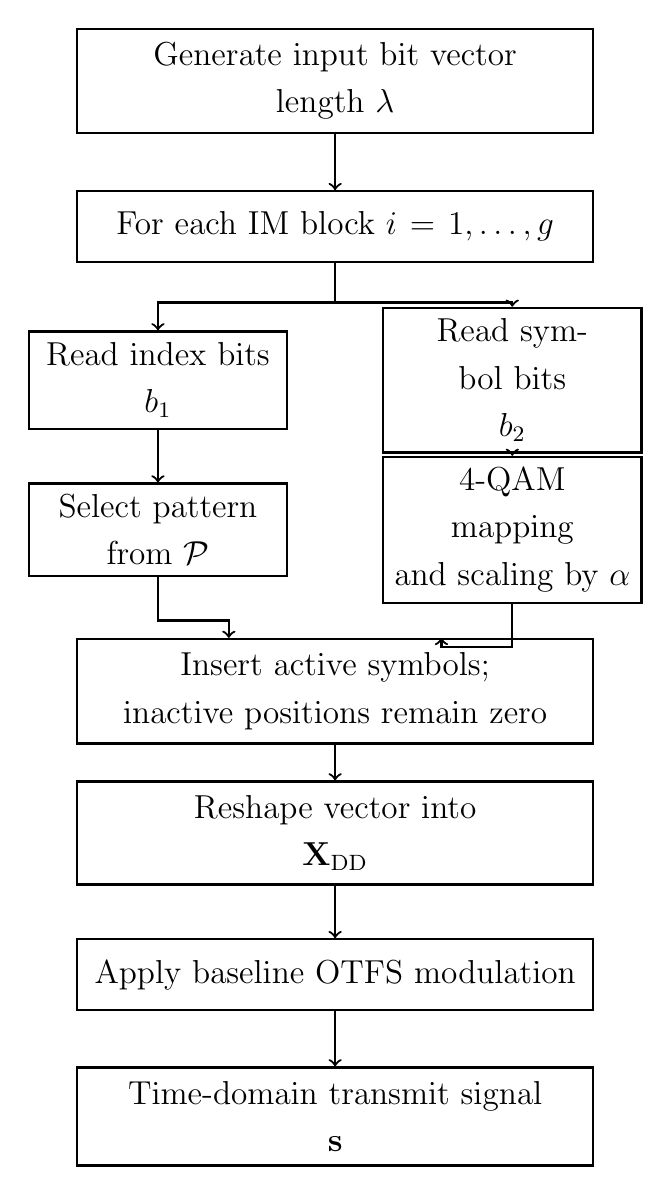
\begin{tikzpicture}[
        block/.style={
            rectangle,
            draw,
            thick,
            align=center,
            text width=6.2cm,
            minimum height=0.9cm,
            font=\small,
            inner sep=5pt
        },
        smallblock/.style={
            rectangle,
            draw,
            thick,
            align=center,
            text width=3.0cm,
            minimum height=0.85cm,
            font=\small,
            inner sep=4pt
        },
        arrow/.style={->, thick}
    ]

        \node[block] (bits) at (0,0) {Generate input bit vector\\length \(\lambda\)};
        \node[block] (loop) at (0,-1.85) {For each IM block \(i=1,\ldots,g\)};
        \node[smallblock] (idx) at (-2.25,-3.8) {Read index bits\\\(b_1\)};
        \node[smallblock] (sym) at (2.25,-3.8) {Read symbol bits\\\(b_2\)};
        \node[smallblock] (pat) at (-2.25,-5.7) {Select pattern\\from \(\mathcal{P}\)};
        \node[smallblock] (qam) at (2.25,-5.7) {4-QAM mapping\\and scaling by \(\alpha\)};
        \node[block] (insert) at (0,-7.75) {Insert active symbols;\\inactive positions remain zero};
        \node[block] (reshape) at (0,-9.55) {Reshape vector into\\\(\mathbf{X}_{\mathrm{DD}}\)};
        \node[block] (otfs) at (0,-11.35) {Apply baseline OTFS modulation};
        \node[block] (tx) at (0,-13.15) {Time-domain transmit signal\\\(\mathbf{s}\)};

        \draw[arrow] (bits.south) -- (loop.north);
        \draw[arrow] (loop.south) -- ++(0,-0.5) -| (idx.north);
        \draw[arrow] (loop.south) -- ++(0,-0.5) -| (sym.north);
        \draw[arrow] (idx.south) -- (pat.north);
        \draw[arrow] (sym.south) -- (qam.north);
        \draw[arrow] (pat.south) -- ++(0,-0.55) -| ([xshift=-1.35cm]insert.north);
        \draw[arrow] (qam.south) -- ++(0,-0.55) -| ([xshift=1.35cm]insert.north);
        \draw[arrow] (insert.south) -- (reshape.north);
        \draw[arrow] (reshape.south) -- (otfs.north);
        \draw[arrow] (otfs.south) -- (tx.north);

    \end{tikzpicture}
    \caption{OTFS-IM transmitter processing flow}
    \label{fig:otfs_im_transmitter_flow}
\end{figure}

This flow also reflects the separation between the proposed OTFS-IM mapping and the baseline OTFS modulation. The index-modulation part determines the sparse delay-Doppler grid, while the modulation part converts this grid into the transmitted time-domain waveform.

\subsubsection{Index and Symbol Bit Mapping}

For the \(i\)-th IM block, the transmitter reads \(b_1\) index bits and converts them into a decimal value. Let this value be denoted by \(q_i\). The implemented mapping then converts \(q_i\) into a Gray index:
\begin{equation}
    m_i
    =
    q_i
    \oplus
    \left\lfloor
    \frac{q_i}{2}
    \right\rfloor ,
    \label{eq:tx_gray_index}
\end{equation}
where \(\oplus\) denotes bitwise exclusive-or.
The selected activation pattern is then obtained from the pattern table:
\begin{equation}
    \mathbf{p}_{m_i}
    =
    \mathcal{P}[m_i].
    \label{eq:tx_pattern_selection}
\end{equation}
The entries of \(\mathbf{p}_{m_i}\) are local active positions inside the current IM block.

The next \(b_2\) bits are used to generate the active QAM symbols. Since
\begin{equation}
    b_2 = k\log_2(M_{\mathrm{mod}}),
\end{equation}
these bits form exactly \(k\) modulation symbols. In this thesis, \(M_{\mathrm{mod}}=4\), so each active position carries one 4-QAM symbol. The generated QAM symbols are multiplied by the normalization factor
\begin{equation}
    \alpha = \sqrt{\frac{n}{k}},
\end{equation}
which preserves the average block energy when only \(k\) out of \(n\) positions are active.

After one IM block is processed, the bit-reading position is advanced by \(b_1+b_2\) bits. This ensures that the input vector is consumed sequentially and that each block carries one index label and \(k\) active QAM symbols.

\subsubsection{Illustrative Block-Mapping Example}

To clarify the mapping process, consider the representative configuration \((n,k)=(4,3)\) with 4-QAM. In this case, there are
\begin{equation}
    \binom{4}{3}=4
\end{equation}
valid constant-weight activation patterns. Therefore,
\begin{equation}
    b_1=\left\lfloor \log_2 4 \right\rfloor=2,
    \qquad
    b_2=3\log_2(4)=6.
\end{equation}
Each IM block carries \(b_1+b_2=8\) information bits. The first two bits select one activation pattern, and the next six bits generate three 4-QAM symbols.

Suppose that the selected activation pattern is
\begin{equation}
    \mathbf{p}_{m_i}=[1,2,4].
\end{equation}
Then the first, second, and fourth local positions of the IM block are active, while the third local position is inactive. If the three scaled QAM symbols for this block are denoted by \(\alpha s_{i,1}\), \(\alpha s_{i,2}\), and \(\alpha s_{i,3}\), the local block vector becomes
\begin{equation}
    \mathbf{x}_{i}
    =
    \left[
    \alpha s_{i,1},
    \alpha s_{i,2},
    0,
    \alpha s_{i,3}
    \right]^{T}.
    \label{eq:otfs_im_local_block_example}
\end{equation}
This example shows the two-layer information structure of OTFS-IM. The nonzero symbol values carry QAM information, while the zero position carries index information because its location is part of the selected activation pattern.

For the next IM block, the same procedure is repeated on the next group of \(n\) delay-Doppler positions. Thus, the full OTFS-IM frame is not one arbitrary sparse vector. It is a structured sparse vector formed by concatenating \(g\) local IM blocks, each of which has exactly \(k\) active positions. This structure is what makes block-wise MAP detection possible at the receiver.

\subsubsection{Delay-Doppler Grid Construction}

The vectorized OTFS-IM delay-Doppler frame is denoted by \(\mathbf{x}_{\mathrm{vec}}\). It has length \(NM\) and is initialized as an all-zero vector:
\begin{equation}
    \mathbf{x}_{\mathrm{vec}} \in \mathbb{C}^{NM \times 1}.
\end{equation}
For the \(i\)-th IM block, the local positions are
\begin{equation}
    \mathcal{B}_i
    =
    \{(i-1)n+1,\ldots,in\}.
\end{equation}
If the selected local active pattern is \(\mathbf{p}_{m_i}\), then the global active positions are
\begin{equation}
    (i-1)n + \mathbf{p}_{m_i}.
    \label{eq:tx_global_active_positions}
\end{equation}
Only these positions are filled with the scaled QAM symbols. In compact form, the assignment can be written as
\begin{equation}
    \mathbf{x}_{\mathrm{vec}}\big((i-1)n+\mathbf{p}_{m_i}\big)
    =
    \alpha \mathbf{s}_i,
    \label{eq:tx_xvec_assignment}
\end{equation}
where \(\mathbf{s}_i\) contains the \(k\) QAM symbols of the \(i\)-th IM block.

All inactive positions remain zero by construction. This choice is simple but important: zeros are not missing symbols; they are intentional inactive resource elements that carry index information through their locations.

After all \(g\) IM blocks have been processed, the vector \(\mathbf{x}_{\mathrm{vec}}\) is reshaped into the \(N \times M\) delay-Doppler grid:
\begin{equation}
    \mathbf{X}_{\mathrm{DD}}
    =
    \mathrm{reshape}
    \left(
    \mathbf{x}_{\mathrm{vec}}, N, M
    \right).
    \label{eq:tx_xdd_reshape}
\end{equation}
This grid is the OTFS-IM counterpart of the full QAM delay-Doppler grid used in the baseline OTFS transmitter. The difference is that \(\mathbf{X}_{\mathrm{DD}}\) now contains both active QAM entries and inactive zero entries.

\subsubsection{Connection to the Baseline OTFS Modulation Block}

Once the OTFS-IM delay-Doppler grid has been constructed, the remaining modulation process is identical to the baseline OTFS transmitter. The OTFS-IM transmit signal can be written compactly as
\begin{equation}
    \mathbf{s}_{\mathrm{IM}}
    =
    \mathcal{M}_{\mathrm{OTFS}}
    \left\{
    \mathbf{X}_{\mathrm{DD}}
    \right\},
    \label{eq:otfs_im_common_modulation}
\end{equation}
where \(\mathcal{M}_{\mathrm{OTFS}}\{\cdot\}\) denotes the common OTFS modulation operation. The delay-Doppler grid is first transformed into the time-frequency domain using the ISFFT operation, and the time-domain transmit signal is then obtained through the discrete Heisenberg transform. Therefore, the transmitter design in this chapter does not redefine the OTFS modulation theory from Chapter 3. Instead, it changes the content of the delay-Doppler input grid before the common OTFS modulation block is applied.

This modular structure is useful for a fair comparison. Baseline OTFS and OTFS-IM share the same frame size, channel model, OTFS modulation and demodulation operations, and detector foundation. The main difference is the delay-Doppler grid construction. Consequently, the simulation results in Chapter 5 can attribute performance differences mainly to the use of index modulation and activation-pattern design rather than to a different physical-layer waveform implementation.


\subsection{OTFS-IM Receiver and Block-Wise MAP Detection}

The OTFS-IM receiver differs from the baseline OTFS receiver because it must recover both the active-position pattern and the QAM symbols placed on the active positions. Therefore, a hard symbol-by-symbol decision is not sufficient. In this thesis, the MP detector is used as a probability engine, and an additional block-wise MAP decision stage is applied to recover the index bits and symbol bits of each IM block.

\subsubsection{Overview of the OTFS-IM Receiver Processing Chain}

After transmission through the delay-Doppler channel, the received time-domain signal is demodulated by the same OTFS demodulation block used in Chapter 3. The output is a delay-Doppler-domain observation denoted by \(\mathbf{Y}_{\mathrm{DD}}\). Since the OTFS-IM transmitter scales active symbols by \(\alpha\), the receiver first normalizes the demodulated grid and the corresponding noise variance:
\begin{equation}
    \mathbf{Y}_{\mathrm{norm}}
    =
    \frac{\mathbf{Y}_{\mathrm{DD}}}{\alpha},
    \qquad
    \sigma^2_{\mathrm{norm}}
    =
    \frac{\sigma^2_{\mathrm{IM}}}{\alpha^2}.
    \label{eq:otfs_im_receiver_normalization}
\end{equation}
The normalized delay-Doppler grid is then passed to the MP detector. The detector estimates, for each delay-Doppler position, the probability that the transmitted value belongs to one of the QAM constellation points or to the inactive value zero. These probabilities are then used by the block-wise MAP stage to decide the most likely activation pattern and active QAM symbols.

Figure~\ref{fig:otfs_im_receiver_flow} summarizes the implemented OTFS-IM receiver flow.

\begin{figure}[H]
    \centering
    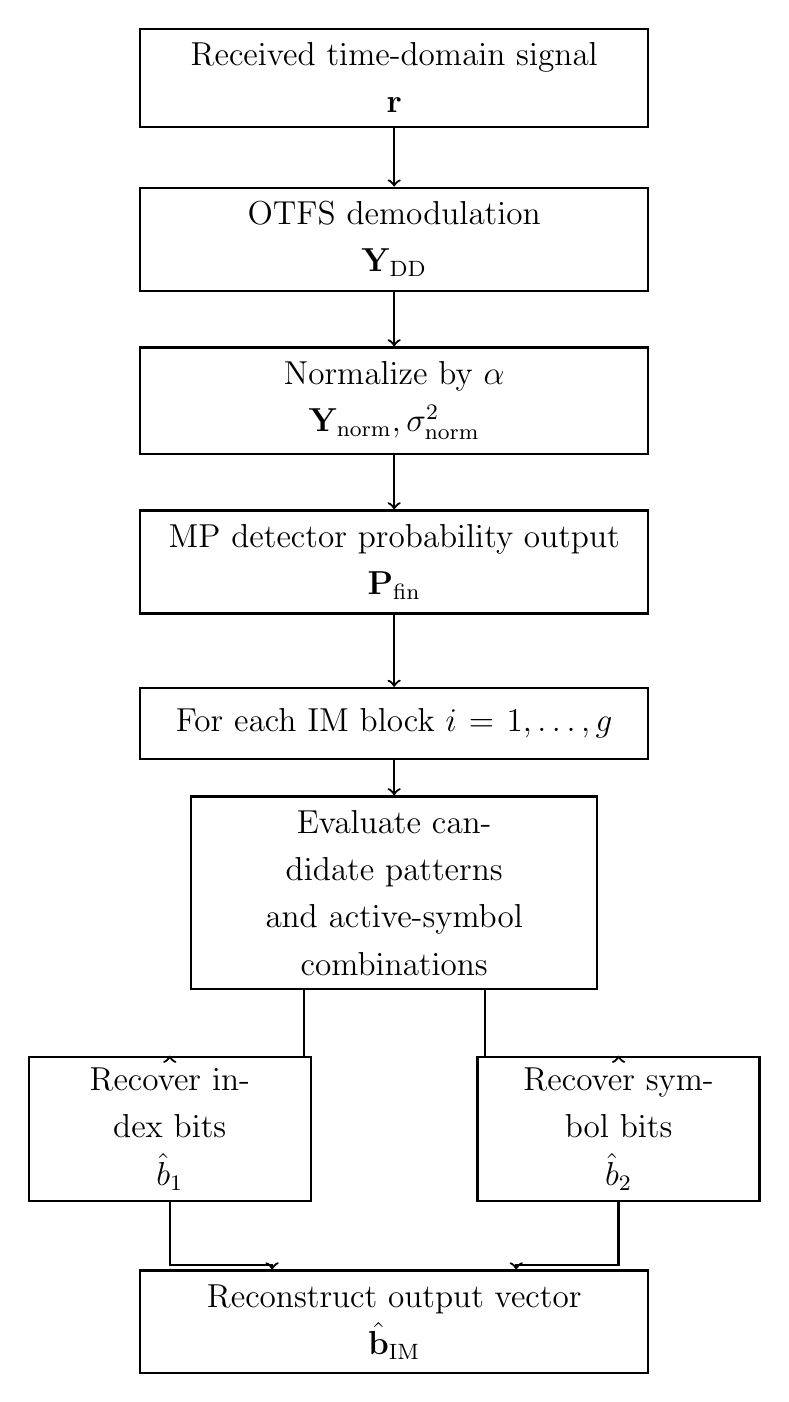
\begin{tikzpicture}[
        block/.style={
            rectangle,
            draw,
            thick,
            align=center,
            text width=6.1cm,
            minimum height=0.9cm,
            font=\small,
            inner sep=5pt
        },
        smallblock/.style={
            rectangle,
            draw,
            thick,
            align=center,
            text width=3.3cm,
            minimum height=0.85cm,
            font=\small,
            inner sep=4pt
        },
        scoreblock/.style={
            rectangle,
            draw,
            thick,
            align=center,
            text width=4.8cm,
            minimum height=0.9cm,
            font=\small,
            inner sep=5pt
        },
        arrow/.style={->, thick}
    ]

        \node[block] (rx) at (0,0) {Received time-domain signal\\\(\mathbf{r}\)};
        \node[block] (demod) at (0,-2.05) {OTFS demodulation\\\(\mathbf{Y}_{\mathrm{DD}}\)};
        \node[block] (norm) at (0,-4.10) {Normalize by \(\alpha\)\\\(\mathbf{Y}_{\mathrm{norm}}, \sigma^2_{\mathrm{norm}}\)};
        \node[block] (mp) at (0,-6.15) {MP detector probability output\\\(\mathbf{P}_{\mathrm{fin}}\)};
        \node[block] (loop) at (0,-8.20) {For each IM block \(i=1,\ldots,g\)};
        \node[scoreblock] (score) at (0,-10.35) {Evaluate candidate patterns\\and active-symbol combinations};
        \node[smallblock] (idx) at (-2.85,-13.35) {Recover index bits\\\(\hat{b}_1\)};
        \node[smallblock] (sym) at (2.85,-13.35) {Recover symbol bits\\\(\hat{b}_2\)};
        \node[block] (bits) at (0,-15.80) {Reconstruct output vector\\\(\hat{\mathbf{b}}_{\mathrm{IM}}\)};

        \draw[arrow] (rx.south) -- (demod.north);
        \draw[arrow] (demod.south) -- (norm.north);
        \draw[arrow] (norm.south) -- (mp.north);
        \draw[arrow] (mp.south) -- (loop.north);
        \draw[arrow] (loop.south) -- (score.north);
        \draw[arrow] ([xshift=-1.15cm]score.south) -- ++(0,-0.85) -| (idx.north);
        \draw[arrow] ([xshift=1.15cm]score.south) -- ++(0,-0.85) -| (sym.north);
        \draw[arrow] (idx.south) -- ++(0,-0.80) -| ([xshift=-1.55cm]bits.north);
        \draw[arrow] (sym.south) -- ++(0,-0.80) -| ([xshift=1.55cm]bits.north);

    \end{tikzpicture}
    \caption{OTFS-IM receiver processing flow with block-wise MAP detection}
    \label{fig:otfs_im_receiver_flow}
\end{figure}

\subsubsection{Probability Output from the MP Detector}

The MP detector used in this thesis is the same detector foundation as in the baseline OTFS system, but its alphabet is extended to include the inactive value. For OTFS-IM, the candidate alphabet is
\begin{equation}
    \mathcal{S}_{0}
    =
    \mathcal{S}
    \cup
    \{0\},
    \label{eq:otfs_im_extended_alphabet}
\end{equation}
where \(\mathcal{S}\) is the 4-QAM constellation and \(0\) represents an inactive delay-Doppler position.

For each resource element, the detector returns a probability vector over the extended alphabet. The final probability matrix is denoted by \(\mathbf{P}_{\mathrm{fin}}\). For one IM block, the receiver extracts two types of probabilities:
\begin{equation}
    p_{0,\ell}
    =
    \Pr(x_\ell=0),
    \qquad
    p_{\ell}(a)
    =
    \Pr(x_\ell=s_a),
    \label{eq:zero_and_symbol_probabilities}
\end{equation}
where \(\ell\) is a local position in the IM block and \(s_a\in\mathcal{S}\) is a QAM candidate symbol. A small lower bound is applied to avoid taking the logarithm of zero during MAP scoring.

This probability-based output is the key reason the same MP detector can be reused for OTFS-IM. The detector does not need to directly output index bits. Instead, it provides enough soft information for the following block-wise MAP stage to determine whether each candidate position is active or inactive.

\subsubsection{Block-Wise MAP Pattern and Symbol Detection}

For the \(i\)-th IM block, the receiver tests every candidate activation pattern stored in the pattern table \(\mathcal{P}\). For a candidate pattern \(\mathbf{p}_m\), the inactive positions are the complement of \(\mathbf{p}_m\) inside the local block. The receiver also tests all possible QAM symbol combinations on the \(k\) active positions.

The likelihood score is computed in the logarithmic domain. For a candidate pattern \(\mathbf{p}_m\) and a candidate symbol vector \(\mathbf{s}\), the score can be written as
\begin{equation}
    \Lambda(m,\mathbf{s})
    =
    \sum_{\ell \in \mathcal{I}_m^{0}}
    \log p_{0,\ell}
    +
    \sum_{u=1}^{k}
    \log p_{p_m(u)}(s_u),
    \label{eq:block_map_score}
\end{equation}
where \(\mathcal{I}_m^{0}\) denotes the inactive positions associated with the candidate pattern. The first term rewards positions that are likely to be inactive, while the second term rewards active positions that are likely to contain the tested QAM symbols.

For each candidate pattern, the receiver keeps the best symbol combination:
\begin{equation}
    \Gamma(m)
    =
    \max_{\mathbf{s}\in\mathcal{S}^{k}}
    \Lambda(m,\mathbf{s}).
    \label{eq:best_symbol_score}
\end{equation}
The detected pattern index is then obtained as
\begin{equation}
    \hat{m}
    =
    \arg\max_m
    \Gamma(m).
    \label{eq:detected_pattern_index}
\end{equation}
Once \(\hat{m}\) is found, the corresponding best QAM symbol combination is also known.

The detected pattern index is converted back to binary index bits through the inverse Gray mapping:
\begin{equation}
    \hat{\mathbf{b}}_{\mathrm{idx}}
    =
    \mathrm{de2bi}
    \left(
    \mathrm{gray\_to\_bin}(\hat{m}), b_1
    \right).
    \label{eq:receiver_index_bits}
\end{equation}
The detected QAM symbol indices are separately converted back to symbol bits. The two bit groups are then concatenated in the same order used by the transmitter:
\begin{equation}
    \hat{\mathbf{b}}_i
    =
    \left[
    \hat{\mathbf{b}}_{\mathrm{idx}}^{T},
    \hat{\mathbf{b}}_{\mathrm{sym}}^{T}
    \right]^{T}.
    \label{eq:receiver_block_bits}
\end{equation}
Repeating this process for all \(g\) IM blocks reconstructs the full received bit vector \(\hat{\mathbf{b}}_{\mathrm{IM}}\).

\subsubsection{MAP Search Complexity and Practical Interpretation}

The block-wise MAP stage is much smaller than a full-frame joint detector because the search is restricted to one IM block at a time. For each block, the receiver tests \(2^{b_1}\) candidate activation patterns. For each candidate pattern, it also evaluates the possible QAM symbol combinations on the \(k\) active positions. Therefore, the number of pattern-symbol hypotheses per IM block is
\begin{equation}
    N_{\mathrm{hyp}}
    =
    2^{b_1}
    |\mathcal{S}|^{k}.
    \label{eq:map_hypothesis_count}
\end{equation}
This expression shows why the block size \(n\), the number of active positions \(k\), and the QAM order must be selected carefully. Increasing \(k\) can improve spectral efficiency, but it also increases the number of active-symbol combinations that must be evaluated during MAP detection.

For the configurations used in this thesis, the MAP search remains practical. With 4-QAM and \((n,k)=(4,3)\), the number of index patterns is \(2^{b_1}=4\) and the number of QAM combinations per pattern is \(4^3=64\). Thus, each block requires \(4\times64=256\) pattern-symbol hypotheses. This is manageable because the decision is performed locally for each IM block rather than jointly over the full \(NM\)-element frame.

The probability output of the MP detector is essential in this process. If the receiver only had hard decisions for each delay-Doppler position, an early wrong decision could force the MAP stage into an incorrect pattern. By using soft probabilities, the receiver can compare competing explanations of the whole block. A position that is uncertain between zero and a QAM symbol is not immediately fixed; instead, its probability contributes to the likelihood score of each candidate pattern.

This is the main reason why the OTFS-IM receiver is described as a two-stage receiver. The first stage converts the channel-distorted delay-Doppler observation into a probability map. The second stage interprets that probability map according to the valid activation-pattern table. The two stages have different roles: MP detection handles sparse channel interference, while block-wise MAP detection handles index-modulation structure.

\subsubsection{Illustrative MAP Scoring Example}

The MAP score in Equation~\eqref{eq:block_map_score} can be interpreted as a consistency check between a candidate pattern and the detector probability map. Consider again a local block with \(n=4\) and \(k=3\). If the candidate pattern is \(\mathbf{p}_m=[1,2,4]\), then the inactive-position set is
\begin{equation}
    \mathcal{I}_{m}^{0}=\{3\}.
\end{equation}
The MAP score for this candidate pattern contains one inactive-position term and three active-symbol terms:
\begin{equation}
    \Lambda(m,\mathbf{s})
    =
    \log p_{0,3}
    +
    \log p_{1}(s_1)
    +
    \log p_{2}(s_2)
    +
    \log p_{4}(s_3).
    \label{eq:map_score_example}
\end{equation}
If the MP detector assigns a high zero probability to the third position and high QAM-symbol probabilities to the first, second, and fourth positions, this candidate pattern receives a strong score. If the detector instead believes that the third position is active, the term \(\log p_{0,3}\) becomes small and the score decreases.

This example highlights why index errors and symbol errors are connected. A wrong activation pattern changes which local positions are interpreted as active, so the QAM symbols may be read from the wrong positions. Conversely, if the active-symbol probabilities are weak, the receiver may prefer another pattern that gives a better total block likelihood. The MAP detector therefore performs joint pattern and symbol recovery at the block level, even though the MP detector first produces position-wise probabilities.

\subsubsection{Error Components for OTFS-IM Evaluation}

The OTFS-IM receiver naturally produces several error components. This is useful because total BER alone does not reveal whether the receiver failed because of an incorrect activation pattern or because of incorrect QAM symbol decisions on the active positions.

The total OTFS-IM BER is computed as
\begin{equation}
    \mathrm{BER}_{\mathrm{IM}}
    =
    \frac{
    N_{\mathrm{err,total}}
    }{
    \lambda N_{\mathrm{frame}}
    }.
    \label{eq:otfs_im_total_ber}
\end{equation}
The index BER is computed using only the recovered index bits:
\begin{equation}
    \mathrm{BER}_{\mathrm{idx}}
    =
    \frac{
    N_{\mathrm{err,idx}}
    }{
    g b_1 N_{\mathrm{frame}}
    },
    \label{eq:otfs_im_index_ber}
\end{equation}
and the symbol BER is computed using only the QAM symbol bits:
\begin{equation}
    \mathrm{BER}_{\mathrm{sym}}
    =
    \frac{
    N_{\mathrm{err,sym}}
    }{
    g b_2 N_{\mathrm{frame}}
    }.
    \label{eq:otfs_im_symbol_ber}
\end{equation}
The pattern error rate is defined as
\begin{equation}
    \mathrm{PER}_{\mathrm{pat}}
    =
    \frac{
    N_{\mathrm{err,pat}}
    }{
    gN_{\mathrm{frame}}
    }.
    \label{eq:otfs_im_pattern_error_rate}
\end{equation}

These quantities are reported in Chapter 5 to support a deeper interpretation of the OTFS-IM results. In particular, when pattern-selection methods are compared, the pattern error rate and index BER are more informative than total BER alone because they directly reflect the reliability of activation-pattern detection.


\subsection{OHD and Balanced-OHD Pattern Selection}

The previous sections described how OTFS-IM uses an activation-pattern table to map index bits into active delay-Doppler positions. This section focuses on how that table is selected. In the original OTFS-IM structure, any subset of valid constant-weight activation patterns can be used as long as the number of selected patterns is \(2^{b_1}\). However, different pattern tables do not necessarily have the same detection reliability. If two patterns are very similar, a small detection error in one position may cause the receiver to select the wrong index pattern. Therefore, pattern-table design becomes an important part of the implemented OTFS-IM system.

In this thesis, two deterministic selection rules are considered. The first one is the OHD method, which selects patterns with the largest minimum Hamming distance. The second one is Balanced-OHD, denoted as B-OHD, which keeps the same primary OHD objective but adds tie-breaking criteria related to average distance and carrier-usage balance.

\subsubsection{Pattern-Selection Problem Formulation}

For an IM block of length \(n\) with \(k\) active positions, the full set of constant-weight patterns is
\begin{equation}
    \mathcal{C}
    =
    \left\{
    \mathbf{p} \subset \{1,2,\ldots,n\}
    \; \middle| \;
    |\mathbf{p}| = k
    \right\}.
    \label{eq:full_pattern_candidate_set}
\end{equation}
The number of candidates is
\begin{equation}
    |\mathcal{C}|
    =
    \binom{n}{k}.
    \label{eq:number_of_candidate_patterns}
\end{equation}
Each candidate pattern contains the active local positions of one IM block. The complete set can be generated by enumerating all \(k\)-element subsets of \(\{1,2,\ldots,n\}\).

Since only \(b_1=\lfloor \log_2 \binom{n}{k} \rfloor\) index bits are assigned to one IM block, the pattern table used for transmission contains
\begin{equation}
    L
    =
    2^{b_1}
    \label{eq:number_of_selected_patterns}
\end{equation}
patterns. The design problem is therefore to select a subset
\begin{equation}
    \mathcal{M}
    \subseteq
    \mathcal{C},
    \qquad
    |\mathcal{M}| = L,
    \label{eq:selected_pattern_subset}
\end{equation}
and store it as the selected pattern table \(\mathcal{P}_{\mathrm{sel}}\), which corresponds to the activation-pattern table \(\mathcal{P}\) used in the transmitter and receiver descriptions. This table maps index bits to active positions at the transmitter and restricts the block-wise MAP search to valid candidate patterns at the receiver.

To evaluate the separation between patterns, each pattern is represented by a binary vector of length \(n\). For a pattern \(\mathbf{p}_i\), its binary representation is denoted by \(\mathbf{a}_i\), where
\begin{equation}
    a_i(\ell)
    =
    \begin{cases}
    1, & \ell \in \mathbf{p}_i,\\
    0, & \ell \notin \mathbf{p}_i.
    \end{cases}
    \label{eq:binary_pattern_representation}
\end{equation}
The Hamming distance between two candidate patterns is then
\begin{equation}
    d_{\mathrm{H}}(\mathbf{p}_i,\mathbf{p}_j)
    =
    \sum_{\ell=1}^{n}
    a_i(\ell) \oplus a_j(\ell),
    \label{eq:ohd_pattern_hamming_distance}
\end{equation}
where \(\oplus\) denotes the exclusive-or operation. The resulting pairwise distances form the Hamming-distance matrix used during pattern-table selection.

\subsubsection{OHD Criterion Based on Hamming Distance}

The purpose of the OHD method is to select a pattern table whose closest pair of patterns is as far apart as possible. For a candidate table \(\mathcal{M}\), the minimum pairwise Hamming distance is
\begin{equation}
    d_{\min}(\mathcal{M})
    =
    \min_{\mathbf{p}_i,\mathbf{p}_j \in \mathcal{M},\, i\neq j}
    d_{\mathrm{H}}(\mathbf{p}_i,\mathbf{p}_j).
    \label{eq:pattern_minimum_hamming_distance}
\end{equation}
The OHD-selected table is obtained by
\begin{equation}
    \mathcal{M}_{\mathrm{OHD}}
    =
    \arg\max_{\mathcal{M}\subseteq\mathcal{C},\,|\mathcal{M}|=L}
    d_{\min}(\mathcal{M}).
    \label{eq:ohd_selection_rule}
\end{equation}
This criterion is simple but meaningful for OTFS-IM detection. If two selected activation patterns differ in many positions, then the receiver must make more position-level mistakes before confusing one pattern with the other. As a result, a larger \(d_{\min}\) is expected to reduce the pattern error rate and, consequently, the index BER.

For exact OHD selection, all candidate pattern subsets are enumerated when the search is computationally feasible. For each subset, the method computes its minimum pairwise Hamming distance and keeps the subset with the largest value. The selected table is then used as the activation-pattern table, while diagnostic quantities such as minimum distance, distance matrix, and balance metrics are retained for analysis.

The OHD rule should be interpreted as a geometry-based table design method rather than a detector modification. It does not change the OTFS modulator, the channel model, or the MP detector equations. Instead, it changes which activation patterns are allowed to represent index bits. This distinction is important for the simulation analysis in Chapter 5, because any performance difference between OHD OTFS-IM and another OTFS-IM pattern table can be traced back to the pattern geometry.

\subsubsection{Balanced-OHD Tie-Breaking Strategy}

In many IM configurations, several candidate pattern tables can have the same maximum minimum Hamming distance. The pure OHD method only guarantees the best value of \(d_{\min}\), but it does not necessarily distinguish between tables that are tied under this primary criterion. Balanced-OHD addresses this limitation by keeping the OHD objective as the first priority and then applying additional tie-breaking rules.

For a selected table \(\mathcal{M}\), the average pairwise Hamming distance is defined as
\begin{equation}
    \bar{d}_{\mathrm{H}}(\mathcal{M})
    =
    \frac{2}{L(L-1)}
    \sum_{i<j}
    d_{\mathrm{H}}(\mathbf{p}_i,\mathbf{p}_j).
    \label{eq:average_hamming_distance}
\end{equation}
The number of closest pairs is
\begin{equation}
    N_{\min}(\mathcal{M})
    =
    \left|
    \left\{
    (i,j): i<j,\,
    d_{\mathrm{H}}(\mathbf{p}_i,\mathbf{p}_j)=d_{\min}(\mathcal{M})
    \right\}
    \right|.
    \label{eq:number_of_minimum_distance_pairs}
\end{equation}
In addition, the carrier-usage vector is
\begin{equation}
    \mathbf{u}
    =
    \sum_{\mathbf{p}_i\in\mathcal{M}}
    \mathbf{a}_i,
    \label{eq:carrier_usage_vector}
\end{equation}
where \(u_\ell\) indicates how many selected patterns use the \(\ell\)-th local position. The implemented balance metrics are
\begin{equation}
    J_{\mathrm{var}}
    =
    \sum_{\ell=1}^{n}
    \left(u_\ell-\bar{u}\right)^2,
    \qquad
    J_{\mathrm{span}}
    =
    \max_\ell u_\ell - \min_\ell u_\ell.
    \label{eq:carrier_usage_balance_metrics}
\end{equation}

The B-OHD method ranks candidate pattern tables in lexicographic order. The first priority is to maximize \(d_{\min}\). If two tables have the same \(d_{\min}\), the method selects the one with larger \(\bar{d}_{\mathrm{H}}\). If the tie still remains, it selects the table with fewer closest pairs \(N_{\min}\). Finally, if the distance statistics are still identical, it chooses the table with smaller carrier-usage variance and smaller carrier-usage span.

Therefore, B-OHD can be expressed conceptually as
\begin{equation}
    \mathcal{M}_{\mathrm{B\text{-}OHD}}
    =
    \arg\operatorname{best}_{\mathcal{M}}
    \left(
    d_{\min},
    \bar{d}_{\mathrm{H}},
    -N_{\min},
    -J_{\mathrm{var}},
    -J_{\mathrm{span}}
    \right).
    \label{eq:balanced_ohd_selection_rule}
\end{equation}
The signs in this expression indicate that larger distance metrics are preferred, while smaller closest-pair and imbalance metrics are preferred.

Figure~\ref{fig:ohd_balanced_pattern_selection_flow} summarizes the implemented OHD and B-OHD selection process.

\begin{figure}[H]
    \centering
    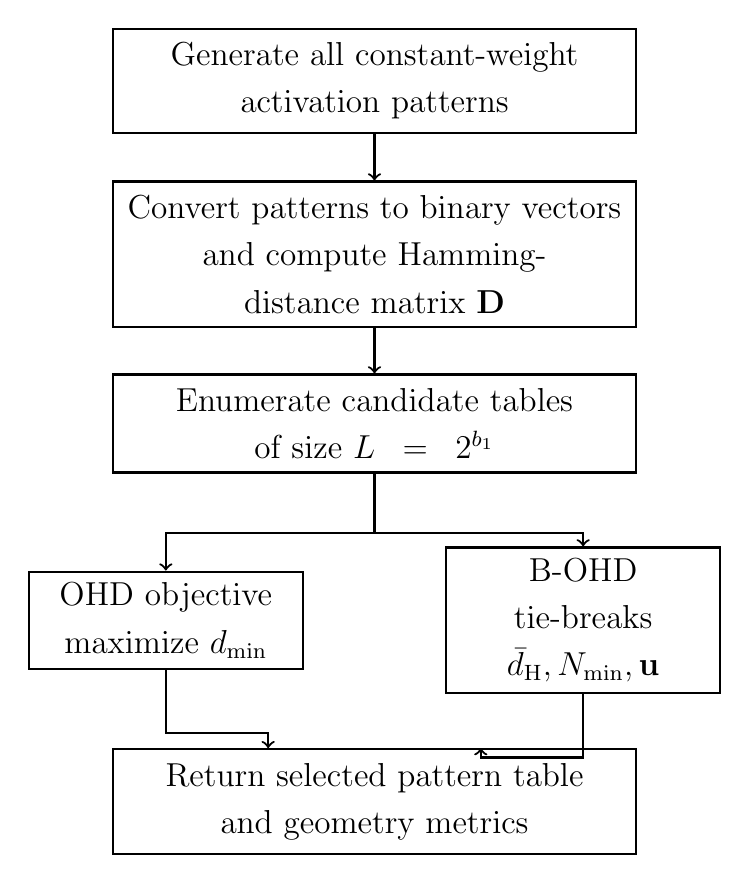
\begin{tikzpicture}[
        block/.style={
            rectangle,
            draw,
            thick,
            align=center,
            text width=6.3cm,
            minimum height=0.9cm,
            font=\small,
            inner sep=5pt
        },
        smallblock/.style={
            rectangle,
            draw,
            thick,
            align=center,
            text width=3.2cm,
            minimum height=0.85cm,
            font=\small,
            inner sep=4pt
        },
        arrow/.style={->, thick}
    ]

        \node[block] (all) at (0,0) {Generate all constant-weight\\activation patterns};
        \node[block] (bin) at (0,-2.20) {Convert patterns to binary vectors\\and compute Hamming-distance matrix \(\mathbf{D}\)};
        \node[block] (sets) at (0,-4.35) {Enumerate candidate tables\\of size \(L=2^{b_1}\)};
        \node[smallblock] (ohd) at (-2.65,-6.85) {OHD objective\\maximize \(d_{\min}\)};
        \node[smallblock] (bohd) at (2.65,-6.85) {B-OHD tie-breaks\\\(\bar{d}_{\mathrm{H}}, N_{\min}, \mathbf{u}\)};
        \node[block] (map) at (0,-9.15) {Return selected pattern table\\and geometry metrics};

        \draw[arrow] (all.south) -- (bin.north);
        \draw[arrow] (bin.south) -- (sets.north);
        \draw[arrow] (sets.south) -- ++(0,-0.75) -| (ohd.north);
        \draw[arrow] (sets.south) -- ++(0,-0.75) -| (bohd.north);
        \draw[arrow] (ohd.south) -- ++(0,-0.80) -| ([xshift=-1.35cm]map.north);
        \draw[arrow] (bohd.south) -- ++(0,-0.80) -| ([xshift=1.35cm]map.north);

    \end{tikzpicture}
    \caption{Pattern-selection flow for OHD and Balanced-OHD}
    \label{fig:ohd_balanced_pattern_selection_flow}
\end{figure}

The purpose of B-OHD is not to claim that carrier balance always dominates the pure OHD choice. Instead, it provides a controlled extension of OHD when multiple tables share the same minimum Hamming distance. This is why Chapter 5 reports OHD and B-OHD separately. If both methods select equivalent or nearly equivalent pattern tables for a given \((n,k)\), their BER curves may overlap. Such a result is not a failure of the method; it means that the selected pattern geometries are effectively the same under that configuration.

\subsubsection{Interpretation of the Pattern-Selection Outputs}

The pattern-selection stage produces more than the selected activation table. It also produces geometry indicators that help explain the BER results in Chapter 5. The most important indicator is \(d_{\min}\), because it describes the closest pair of patterns in the selected table. A larger \(d_{\min}\) generally means that a larger number of position-level mistakes is required before one valid index label can be confused with another.

The average Hamming distance \(\bar{d}_{\mathrm{H}}\) provides a complementary view. While \(d_{\min}\) focuses on the worst-separated pair, the average distance describes the overall separation of the selected table. Two tables can have the same \(d_{\min}\) but different average distances. In that case, B-OHD may prefer the table whose patterns are more separated on average, even if the worst-case pair is unchanged.

The number of closest pairs \(N_{\min}\) is also useful. If many pattern pairs achieve the minimum distance, the receiver has many vulnerable pattern confusions. If only one or two pairs are at the minimum distance, the weak part of the table is more localized. This distinction can affect the pattern error rate, especially at moderate SNR values where the MP probability map is informative but not yet fully reliable.

Finally, the carrier-usage vector \(\mathbf{u}\) indicates whether some local positions are used much more frequently than others. Strong imbalance is not always harmful by itself, but it may make the selected table less robust when certain positions have less reliable probability estimates. The balance metrics in B-OHD therefore serve as secondary tie-breakers, not as replacements for Hamming-distance separation.

\begin{table}[H]
\centering
\caption{Interpretation of pattern-selection criteria.}
\label{tab:pattern_selection_criteria_interpretation}
\begin{tabularx}{0.95\linewidth}{|p{3.2cm}|X|}
\hline
\textbf{Criterion} & \textbf{Interpretation in OTFS-IM detection} \\
\hline
\(d_{\min}\) & Worst-case separation between selected activation patterns; directly related to the most vulnerable pattern confusion. \\
\hline
\(\bar{d}_{\mathrm{H}}\) & Average geometric separation of the selected table; useful when several tables share the same \(d_{\min}\). \\
\hline
\(N_{\min}\) & Number of pattern pairs at the minimum distance; fewer closest pairs means fewer weakest confusions. \\
\hline
\(J_{\mathrm{var}}\), \(J_{\mathrm{span}}\) & Balance of local resource usage across the selected table; used only as secondary tie-breakers in B-OHD. \\
\hline
Random baseline & Diagnostic reference for checking whether deterministic table selection is actually beneficial. \\
\hline
\end{tabularx}
\end{table}

This interpretation is important because a lower total BER should not be attributed to OHD or B-OHD blindly. The selected table must also be examined through its geometry. If the selected tables have the same \(d_{\min}\), similar average distance, and similar carrier-usage statistics, then similar BER behavior is expected. Conversely, if one table has a clearly better distance profile, improvement in pattern error rate and index BER becomes more meaningful.

\subsubsection{Search Complexity and Random Diagnostic Baseline}

The exact OHD and B-OHD implementations enumerate all possible pattern tables of size \(L\) from \(\binom{n}{k}\) candidates. The number of candidate tables is
\begin{equation}
    N_{\mathrm{set}}
    =
    \binom{\binom{n}{k}}{L}.
    \label{eq:pattern_search_complexity}
\end{equation}
This search is acceptable for the small and moderate IM configurations used in this thesis, but it grows rapidly as \(n\) and \(k\) increase. For this reason, the implementation includes a guard condition that stops the exact search when the number of candidate tables exceeds a practical threshold. This keeps the simulation workflow focused on interpretable thesis configurations rather than on large-scale combinatorial optimization.

The simulation framework also includes a random-pattern diagnostic baseline. This baseline does not represent a proposed method. Its role is to test whether the deterministic pattern-selection rule provides a meaningful advantage over arbitrary valid pattern tables. In other words, random selection is used as an evaluation tool, not as a final design choice. If OHD or B-OHD gives lower pattern error rate and index BER than the random average, the result supports the claim that pattern geometry matters. If the random average is similar or better in some configurations, the result must be reported honestly and interpreted as a limitation of pure distance-based pattern selection for that configuration.

This distinction is important for the final evaluation. The baseline OTFS curve shows the effect of adding index modulation to OTFS. The OHD and B-OHD curves show the effect of deterministic pattern-table design inside OTFS-IM. The random-pattern curve, when enabled, checks whether the observed behavior is genuinely caused by the proposed table design or merely by the use of any valid activation-pattern subset.


\subsection{Design Discussion and Chapter Summary}

This section summarizes the OTFS-IM design developed in this chapter and clarifies how it will be evaluated in Chapter 5. The purpose is not to introduce another processing block, but to connect the design choices into one coherent interpretation: OTFS-IM changes the information mapping in the delay-Doppler domain, while OHD and B-OHD change the geometry of the activation-pattern table used by that mapping.

\subsubsection{Summary of the OTFS-IM Design Chain}

The implemented OTFS-IM system is built as an extension of the baseline OTFS transceiver described in Chapter 3. The baseline OTFS modulation and demodulation blocks are reused. The main modification is introduced before OTFS modulation, where the full delay-Doppler QAM grid is replaced by a sparse index-modulated grid. In each IM block, \(b_1\) bits select an activation pattern and \(b_2\) bits select the QAM symbols transmitted on the active positions.

This structure gives OTFS-IM two information-bearing mechanisms. The first one is conventional symbol modulation, represented by the QAM symbols placed on active delay-Doppler positions. The second one is index modulation, represented by the locations of those active positions. Therefore, the receiver cannot simply demodulate QAM symbols independently. It must also infer which activation pattern was transmitted in each block. This is why the MP detector is used to produce soft probability information, and a block-wise MAP stage is then applied to jointly recover index bits and symbol bits.

Table~\ref{tab:chapter4_design_summary} summarizes the main design elements introduced in this chapter and their roles in the implemented simulation model.

\begin{table}[H]
    \centering
    \caption{Summary of the implemented OTFS-IM design elements}
    \label{tab:chapter4_design_summary}
    \begin{tabularx}{\linewidth}{>{\RaggedRight\arraybackslash}p{3.2cm}
                                  >{\RaggedRight\arraybackslash}X
                                  >{\RaggedRight\arraybackslash}p{3.2cm}}
        \toprule
        Design element & Role in the OTFS-IM system & Main evaluation aspect \\
        \midrule
        IM block \((n,k)\) &
        Defines how many positions are available and how many of them are active in each block. &
        Spectral efficiency and sparsity level \\
        \midrule
        Activation-pattern table \(\mathcal{P}\) &
        Maps index bits to valid activation patterns and constrains the receiver MAP search. &
        Pattern error rate and index BER \\
        \midrule
        Power normalization \(\alpha\) &
        Compensates for the fact that only \(k\) out of \(n\) positions carry active QAM symbols. &
        Fairness of BER comparison \\
        \midrule
        MP probability output &
        Provides soft probabilities for QAM symbols and the inactive zero state. &
        Reliability of block-wise decisions \\
        \midrule
        Block-wise MAP decision &
        Recovers the most likely activation pattern and active QAM symbols per IM block. &
        Total BER, index BER, symbol BER \\
        \midrule
        OHD and B-OHD selection &
        Select deterministic pattern tables based on Hamming-distance geometry and balance criteria. &
        Pattern reliability and random baseline validation \\
        \bottomrule
    \end{tabularx}
\end{table}

The most important point from Table~\ref{tab:chapter4_design_summary} is that OTFS-IM is not only a modulation-rate modification. It changes the error structure of the receiver. A wrong activation pattern produces index-bit errors and may also place detected QAM symbols in the wrong positions. For this reason, the simulation study must report more than total BER. The separate index BER, symbol BER, and pattern error rate are necessary to explain why one configuration performs better or worse than another.

\subsubsection{BER-SE Trade-Off and Pattern Reliability}

The use of index modulation creates a trade-off between spectral efficiency and reliability. For one IM block, the number of transmitted bits is \(b_1+b_2\), while the block occupies \(n\) delay-Doppler positions. Thus, the spectral efficiency of the OTFS-IM mapping is controlled by the block parameters \((n,k)\):
\begin{equation}
    \eta_{\mathrm{IM}}
    =
    \frac{b_1+b_2}{n}.
    \label{eq:chapter4_im_se_summary}
\end{equation}
Increasing the number of active positions generally increases the number of QAM symbol bits, while changing \(n\) and \(k\) also changes the number of index bits. However, a higher spectral efficiency does not automatically imply a better system. If the chosen patterns are difficult to distinguish, the additional index bits may increase the error rate.

This is the reason OHD and B-OHD are included in the design. Their purpose is to make the activation patterns more distinguishable. The OHD method focuses on the minimum Hamming distance between selected patterns, while B-OHD additionally considers average distance, the number of closest pairs, and carrier-usage balance. These criteria are not expected to remove all detection errors, especially at low SNR where the MP detector itself may produce uncertain probability estimates. Instead, they aim to reduce pattern confusion when the receiver has enough information to benefit from a better pattern geometry.

Therefore, the final evaluation should be read in two layers. The first layer compares baseline OFDM-LMMSE, baseline OTFS, and OTFS-IM to show the effect of moving from conventional multicarrier transmission to delay-Doppler modulation and then to index modulation. The second layer compares OHD, B-OHD, and the random-pattern diagnostic baseline to show whether deterministic pattern selection improves the reliability of OTFS-IM. If a random pattern table performs close to or better than OHD in some configuration, that result should not be hidden. It indicates that minimum-distance selection alone is not always sufficient and that the benefit of OHD depends on the selected \((n,k)\) setting.

\subsubsection{Quantities to Track in the OTFS-IM Evaluation}

Because OTFS-IM has both symbol-domain and index-domain information, the simulation must track several quantities at the same time. These quantities are not interchangeable. Spectral efficiency explains how many bits are transmitted per delay-Doppler resource element, total BER describes end-to-end bit reliability, and pattern error rate describes whether the receiver selected the correct activation pattern. If only one of these quantities is reported, the behavior of the system can be misinterpreted.

\begin{table}[H]
\centering
\caption{Main quantities used to interpret OTFS-IM results.}
\label{tab:otfs_im_evaluation_quantities}
\begin{tabularx}{0.95\linewidth}{|p{3.0cm}|X|}
\hline
\textbf{Quantity} & \textbf{Reason for reporting} \\
\hline
\(\eta_{\mathrm{IM}}\) & Shows whether an OTFS-IM configuration is rate-fair with baseline OTFS or belongs to a lower-rate reliability-oriented setting. \\
\hline
\(\mathrm{BER}_{\mathrm{IM}}\) & Measures the final end-to-end bit error probability after both index and symbol bits are reconstructed. \\
\hline
\(\mathrm{BER}_{\mathrm{idx}}\) & Isolates errors caused by incorrect recovery of the activation-pattern label. \\
\hline
\(\mathrm{BER}_{\mathrm{sym}}\) & Isolates errors in the QAM symbol bits on positions detected as active. \\
\hline
\(\mathrm{PER}_{\mathrm{pat}}\) & Measures block-level activation-pattern confusion, which is directly affected by pattern-table geometry. \\
\hline
\end{tabularx}
\end{table}

Table~\ref{tab:otfs_im_evaluation_quantities} is also useful for avoiding an overly simple conclusion. A configuration may have low total BER because it transmits fewer bits per block. Another configuration may have higher BER but preserve the same spectral efficiency as baseline OTFS. Similarly, a pattern table may reduce pattern error rate while the total BER remains limited by QAM symbol errors. The evaluation in Chapter 5 is therefore designed to connect these quantities rather than judge the system from a single curve.

\subsubsection{Connection to Chapter 5 Simulation Results}

The design in this chapter directly determines the structure of the simulation results in Chapter 5. The BER overview figure compares OFDM-LMMSE, baseline OTFS, OHD OTFS-IM, and B-OHD OTFS-IM under the same channel and SNR settings. The OTFS-IM error-decomposition figure then separates total BER into index BER, symbol BER, and pattern error rate so that the source of the errors can be identified. The pattern-geometry figure connects the selected activation table to Hamming-distance and carrier-usage properties. Finally, the random-pattern validation figure checks whether the proposed deterministic tables are actually better than arbitrary valid pattern selections.

This evaluation structure follows directly from the design logic of the chapter. If OTFS-IM improves BER at a comparable or higher spectral efficiency, the result supports the usefulness of index modulation in the delay-Doppler domain. If OHD or B-OHD reduces pattern error rate or index BER compared with random selection, the result supports the importance of pattern geometry. If the improvement is small or configuration-dependent, the result still has value because it identifies the limitation of the selected pattern design and motivates further work on detector-aware or channel-aware pattern selection.

In summary, this chapter has developed the OTFS-IM system used in the thesis simulations. It defined the IM block structure, spectral-efficiency expression, activation-pattern mapping, transmitter and receiver processing chains, block-wise MAP recovery, and the OHD/B-OHD pattern-selection methods. These elements provide the technical foundation for Chapter 5, where the proposed OTFS-IM design is evaluated through BER performance, error decomposition, pattern reliability, and BER-SE trade-off analysis.

\newpage


\newpage

\section*{\shortstack[c]{CHAPTER 5. SIMULATION RESULTS AND PERFORMANCE\\[0.18cm]EVALUATION}}
\addcontentsline{toc}{section}{CHAPTER 5. SIMULATION RESULTS AND PERFORMANCE EVALUATION}

% =========================================================
% Numbering for Chapter 5
% =========================================================
\setcounter{section}{5}
\setcounter{subsection}{0}
\setcounter{subsubsection}{0}
\setcounter{figure}{0}
\setcounter{table}{0}
\setcounter{equation}{0}

\renewcommand{\thefigure}{5.\arabic{figure}}
\renewcommand{\thetable}{5.\arabic{table}}
\renewcommand{\theequation}{5.\arabic{equation}}
\renewcommand{\theHfigure}{5.\arabic{figure}}
\renewcommand{\theHtable}{5.\arabic{table}}
\renewcommand{\theHequation}{5.\arabic{equation}}

% =========================================================
% Chapter Introduction
% =========================================================
This chapter evaluates the baseline OFDM-LMMSE system, the baseline OTFS system, and the proposed OTFS-IM schemes under a common delay-Doppler channel simulation framework. The purpose is not only to compare final BER curves, but also to explain how index modulation changes the error structure of the receiver. Therefore, the results are organized from general BER comparison to equal-spectral-efficiency analysis, error decomposition, pattern-selection validation, and finally BER-SE trade-off across several \((n,k)\) configurations. This structure follows the design logic of Chapters 3 and 4 and is consistent with previous studies showing that OTFS detection and OTFS-IM performance depend jointly on channel sparsity, detector reliability, and activation-pattern design~\cite{Raviteja2018OTFSMP,Wu2024OTFSIMDetector,Liang2020OTFSIM}.

% =========================================================
% Chapter Sections
% =========================================================
% !TEX root = ../../main.tex

\subsection{Simulation Setup and Evaluation Metrics}

This section defines the simulation setting used to evaluate the baseline OFDM-LMMSE system, the baseline OTFS system, and the proposed OTFS-IM schemes. The purpose is to make the numerical results in the following sections reproducible and rate-aware. Since OTFS-IM changes both the signal structure and the number of information bits carried by each delay-Doppler block, the evaluation cannot rely only on BER curves. The simulation setup must also specify the spectral efficiency of each configuration and the error components associated with index modulation.

\subsubsection{Simulation Parameters}

All schemes are evaluated over the same delay-Doppler channel realization model and the same \(E_b/N_0\) range. The OTFS frame consists of \(N=10\) Doppler bins and \(M=12\) delay bins, resulting in \(NM=120\) resource elements per frame. The baseline OTFS and OFDM systems use 4-QAM modulation over all resource elements. The OTFS-IM system also uses 4-QAM on active positions, while additional information is conveyed by the activation pattern inside each IM block.

The channel is modeled as a discrete time-varying multipath channel with three propagation paths. The implemented delay taps are \([0,1,2]\), while the Doppler taps are randomly generated integer values in the simulated Doppler grid. Therefore, the simulation represents a Doppler-spread doubly selective channel rather than a channel tied to a specific physical velocity value. This choice is consistent with the purpose of the thesis: evaluating OTFS and OTFS-IM under delay-Doppler channel variations associated with high-mobility communication scenarios, without claiming a particular vehicular speed.

Table~\ref{tab:chapter5_simulation_parameters} summarizes the main simulation parameters used in the numerical evaluation.

\begin{table}[H]
    \centering
    \caption{Main simulation parameters}
    \label{tab:chapter5_simulation_parameters}
    \begin{tabularx}{\linewidth}{>{\RaggedRight\arraybackslash}p{4.4cm}
                                  >{\RaggedRight\arraybackslash}p{4.2cm}
                                  >{\RaggedRight\arraybackslash}X}
        \toprule
        Parameter & Value & Role in the simulation \\
        \midrule
        Doppler bins, \(N\) & 10 & Number of Doppler-domain grid points per OTFS frame \\
        \midrule
        Delay bins, \(M\) & 12 & Number of delay-domain grid points per OTFS frame \\
        \midrule
        Total resource elements & \(NM=120\) & Number of transmitted grid symbols per frame \\
        \midrule
        Baseline modulation & 4-QAM & Modulation used by OFDM-LMMSE and baseline OTFS \\
        \midrule
        Active-symbol modulation in OTFS-IM & 4-QAM & Modulation used on active IM positions \\
        \midrule
        Channel model & 3-tap delay-Doppler channel & Common channel model for OFDM, OTFS, and OTFS-IM \\
        \midrule
        Delay taps & \([0,1,2]\) & Discrete multipath delay positions \\
        \midrule
        Doppler taps & Random integer Doppler taps & Time variation and Doppler-spread behavior \\
        \midrule
        \(E_b/N_0\) range & \(0:5:20\) dB & SNR range used for BER curves \\
        \midrule
        OFDM-LMMSE frames & 1000 & Number of simulated OFDM frames per SNR point \\
        \midrule
        OTFS and OTFS-IM frames & 1000 & Number of simulated OTFS/OTFS-IM frames per SNR point \\
        \midrule
        Random-pattern diagnostic & 5 tables, 100 frames/table & Validation baseline for pattern-selection methods \\
        \bottomrule
    \end{tabularx}
\end{table}

The tested OTFS-IM configurations are selected to cover both equal-rate and reliability-oriented cases. Equal-rate configurations have the same spectral efficiency as the baseline OTFS system, while lower-rate configurations are included to show how reducing the number of transmitted bits per resource element can affect BER. For an IM block with \(n\) positions and \(k\) active positions, the number of index bits per block is
\begin{equation}
    b_1 = \left\lfloor \log_2 \binom{n}{k} \right\rfloor,
    \label{eq:chapter5_index_bits}
\end{equation}
and the number of active-symbol bits per block is
\begin{equation}
    b_2 = k \log_2 M_{\mathrm{QAM}}.
    \label{eq:chapter5_symbol_bits}
\end{equation}
Since 4-QAM is used in this thesis, \(\log_2 M_{\mathrm{QAM}}=2\). The spectral efficiency of the OTFS-IM mapping is then
\begin{equation}
    \eta_{\mathrm{IM}} = \frac{b_1+b_2}{n}.
    \label{eq:chapter5_im_spectral_efficiency}
\end{equation}

\begin{figure}[H]
    \centering
    \resizebox{0.98\linewidth}{!}{%
    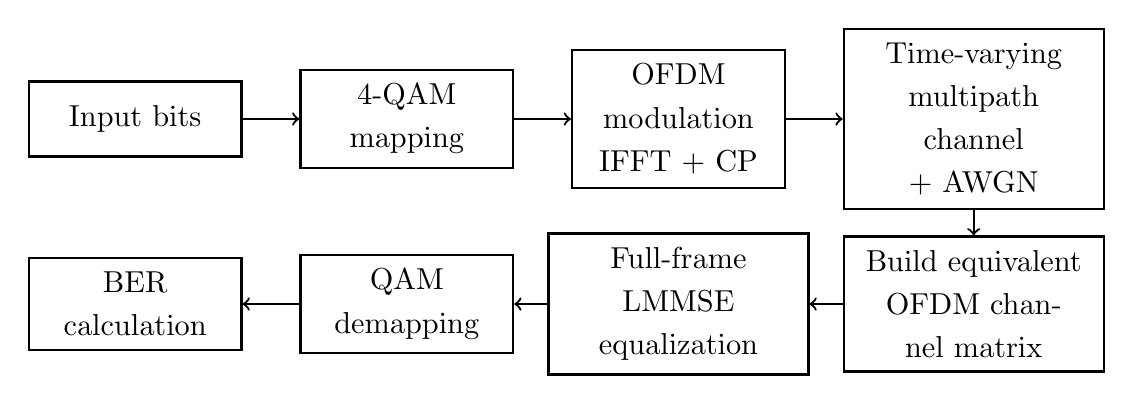
\begin{tikzpicture}[
        block/.style={
            rectangle,
            draw,
            thick,
            align=center,
            text width=2.35cm,
            minimum height=0.95cm,
            font=\footnotesize,
            inner sep=5pt
        },
        wideblock/.style={
            rectangle,
            draw,
            thick,
            align=center,
            text width=2.95cm,
            minimum height=0.95cm,
            font=\footnotesize,
            inner sep=5pt
        },
        arrow/.style={->, thick}
    ]
        \node[block] (bits) at (0,0) {Input bits};
        \node[block] (qam) at (3.45,0) {4-QAM\\mapping};
        \node[block] (ofdm) at (6.90,0) {OFDM\\modulation\\IFFT + CP};
        \node[wideblock] (chan) at (10.65,0) {Time-varying\\multipath channel\\+ AWGN};
        \node[wideblock] (hmat) at (10.65,-2.35) {Build equivalent\\OFDM channel matrix};
        \node[wideblock] (lmmse) at (6.90,-2.35) {Full-frame\\LMMSE equalization};
        \node[block] (demap) at (3.45,-2.35) {QAM\\demapping};
        \node[block] (ber) at (0,-2.35) {BER\\calculation};

        \draw[arrow] (bits.east) -- (qam.west);
        \draw[arrow] (qam.east) -- (ofdm.west);
        \draw[arrow] (ofdm.east) -- (chan.west);
        \draw[arrow] (chan.south) -- (hmat.north);
        \draw[arrow] (hmat.west) -- (lmmse.east);
        \draw[arrow] (lmmse.west) -- (demap.east);
        \draw[arrow] (demap.west) -- (ber.east);
    \end{tikzpicture}
    }
    \caption{OFDM-LMMSE baseline simulation flow}
    \label{fig:chapter5_ofdm_lmmse_flow}
\end{figure}

The OFDM-LMMSE flow in Fig.~\ref{fig:chapter5_ofdm_lmmse_flow} clarifies how the conventional multicarrier baseline is generated in the simulation. The receiver does not simply apply one-tap equalization; instead, it uses a full-frame LMMSE equalizer with channel knowledge. This makes the OFDM reference a stronger baseline for comparison with the delay-Doppler OTFS and OTFS-IM receivers.

Table~\ref{tab:chapter5_im_configurations} lists all simulated OTFS-IM configurations. The baseline OTFS and OFDM-LMMSE systems both have spectral efficiency \(2.00\) bits/symbol under 4-QAM transmission.

\begin{table}[H]
    \centering
    \caption{Simulated OTFS-IM configurations}
    \label{tab:chapter5_im_configurations}
    \begin{tabularx}{\linewidth}{>{\centering\arraybackslash}p{2.4cm}
                                  >{\centering\arraybackslash}p{1.4cm}
                                  >{\centering\arraybackslash}p{1.4cm}
                                  >{\centering\arraybackslash}p{1.4cm}
                                  >{\centering\arraybackslash}p{1.4cm}
                                  >{\centering\arraybackslash}p{2.4cm}
                                  >{\RaggedRight\arraybackslash}X}
        \toprule
        Configuration & \(n\) & \(k\) & \(b_1\) & \(b_2\) & \(\eta_{\mathrm{IM}}\) & Interpretation \\
        \midrule
        \(4\)-\(2\) & 4 & 2 & 2 & 4 & 1.50 & Lower-SE reliability-oriented case \\
        \midrule
        \(4\)-\(3\) & 4 & 3 & 2 & 6 & 2.00 & Equal-SE case \\
        \midrule
        \(5\)-\(3\) & 5 & 3 & 3 & 6 & 1.80 & Main pattern-selection validation case \\
        \midrule
        \(5\)-\(4\) & 5 & 4 & 2 & 8 & 2.00 & Equal-SE case \\
        \midrule
        \(6\)-\(3\) & 6 & 3 & 4 & 6 & 1.67 & Lower-SE reliability-oriented case \\
        \midrule
        \(6\)-\(4\) & 6 & 4 & 3 & 8 & 1.83 & Supplementary trade-off case \\
        \midrule
        \(6\)-\(5\) & 6 & 5 & 2 & 10 & 2.00 & Main larger-block equal-SE case \\
        \bottomrule
    \end{tabularx}
\end{table}

\subsubsection{Compared Schemes and Evaluation Metrics}

Four main schemes are compared in Chapter 5. The first one is OFDM-LMMSE, which is used as the conventional multicarrier reference. In the implementation, OFDM symbols are transmitted over the same time-varying channel as OTFS, and the receiver applies a full-frame LMMSE equalizer with perfect channel knowledge. Therefore, the OFDM curve should be understood as an equalized OFDM baseline, not as an unequalized OFDM receiver. This makes the comparison more meaningful because OTFS and OTFS-IM are not compared against an intentionally weak OFDM receiver.

The second scheme is the baseline OTFS system developed in Chapter 3. It uses full-grid 4-QAM mapping in the delay-Doppler domain and serves as the direct reference for evaluating whether OTFS-IM provides a useful improvement. The third scheme is OHD OTFS-IM, where the activation-pattern table is selected according to the optimized Hamming-distance criterion. The fourth scheme is B-OHD OTFS-IM, where the pattern-selection process additionally considers balance-related criteria such as carrier usage and closest-pair behavior. In configurations where OHD and B-OHD select effectively the same pattern set, their BER curves can overlap. This is not a simulation error; it means that the additional B-OHD criteria do not change the selected table for that specific \((n,k)\) setting.

Random pattern tables are also simulated as a diagnostic baseline. They are not treated as a proposed transmission method. Their role is to test whether deterministic pattern selection actually gives a meaningful advantage over arbitrary valid pattern choices. If a random table performs close to OHD or B-OHD in some SNR region, the result should be interpreted as evidence that pattern geometry alone is not always sufficient to determine the final BER.

The primary performance metric is the total bit error rate,
\begin{equation}
    \mathrm{BER} = \frac{N_{\mathrm{err}}}{N_{\mathrm{bits}}},
    \label{eq:chapter5_ber_definition}
\end{equation}
where \(N_{\mathrm{err}}\) is the number of incorrectly detected bits and \(N_{\mathrm{bits}}\) is the total number of transmitted information bits. For OTFS and OFDM, this BER directly measures the reliability of QAM symbol detection. For OTFS-IM, the total BER contains both index-bit errors and symbol-bit errors.

To explain the OTFS-IM behavior more clearly, the total BER is decomposed into index BER and symbol BER. Index BER measures the reliability of recovering the activation-pattern bits \(b_1\), while symbol BER measures the reliability of recovering the QAM bits \(b_2\) placed on active positions. In addition, the pattern error rate is reported as
\begin{equation}
    \mathrm{PER} = \frac{N_{\mathrm{wrong\ pattern}}}{N_{\mathrm{IM\ blocks}}},
    \label{eq:chapter5_pattern_error_rate}
\end{equation}
where \(N_{\mathrm{wrong\ pattern}}\) is the number of IM blocks in which the selected activation pattern is detected incorrectly. This metric is important because a wrong pattern decision can cause both index errors and symbol-placement errors.

Finally, spectral efficiency is used to distinguish equal-rate gains from rate-reliability trade-offs. A BER reduction is strongest when it is obtained at \(\eta_{\mathrm{IM}}=2.00\) bits/symbol, because this matches the spectral efficiency of the baseline OTFS system. If a configuration has lower BER but also lower spectral efficiency, the result is still useful, but it should be interpreted as a reliability-oriented trade-off rather than an unconditional improvement. For this reason, the final part of Chapter 5 presents both a configuration-level BER summary and a BER-SE trade-off plot across all simulated configurations.


% !TEX root = ../../main.tex

\subsection{Baseline BER Performance Comparison}

After defining the simulation setup, the first performance comparison is made between the conventional OFDM-LMMSE baseline, the baseline OTFS system, and the proposed OTFS-IM schemes. This comparison establishes the main BER trend before the detailed index-modulation analysis is presented. The representative configuration used in this section is \(n=6\), \(k=5\), because it has the same spectral efficiency as the baseline OTFS system:
\begin{equation}
    \eta_{\mathrm{IM}} = \eta_{\mathrm{OTFS}} = 2.00~\mathrm{bits/symbol}.
    \label{eq:chapter5_equal_se_65}
\end{equation}
Therefore, the BER comparison in this section is rate-fair. Any BER improvement of OTFS-IM over OTFS in this configuration is not obtained by reducing the number of transmitted bits per resource element.

\IfFileExists{Images/Chapter5/ber_overview_n6_k5.png}{%
\begin{figure}[H]
    \centering
    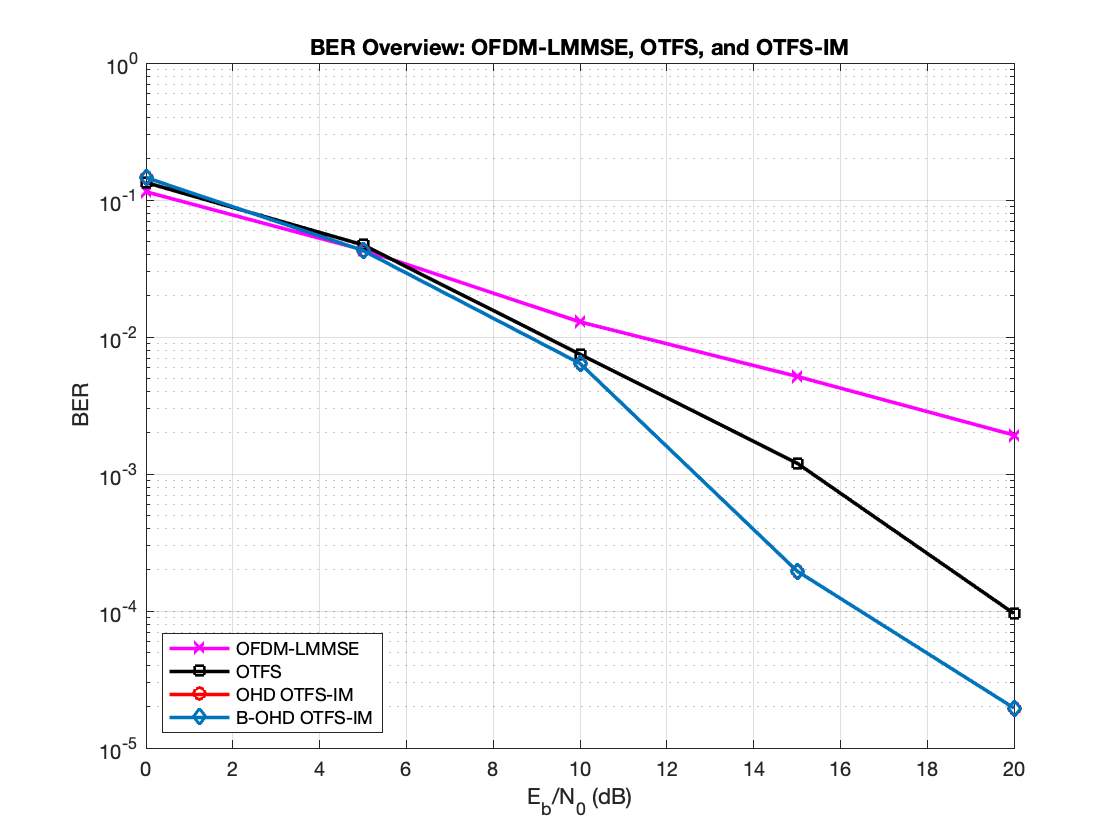
\includegraphics[width=0.88\linewidth]{Images/Chapter5/ber_overview_n6_k5.png}
    \caption{BER overview of OFDM-LMMSE, OTFS, and OTFS-IM for the \(n=6,k=5\) equal-SE configuration}
    \label{fig:chapter5_ber_overview_n6_k5}
\end{figure}
}{%
\begin{figure}[H]
    \centering
    \fbox{\begin{minipage}[c][5cm][c]{0.86\linewidth}
        \centering
        Required figure file is missing:\\
        Images/Chapter5/ber\_overview\_n6\_k5.png
    \end{minipage}}
    \caption{BER overview of OFDM-LMMSE, OTFS, and OTFS-IM for the \(n=6,k=5\) equal-SE configuration}
    \label{fig:chapter5_ber_overview_n6_k5}
\end{figure}
}

Figure~\ref{fig:chapter5_ber_overview_n6_k5} compares the BER of OFDM-LMMSE, baseline OTFS, OHD OTFS-IM, and B-OHD OTFS-IM over the simulated \(E_b/N_0\) range. The OFDM-LMMSE curve is included as the conventional multicarrier reference. Since it uses a full-frame LMMSE equalizer with perfect channel knowledge in the simulation, it should be interpreted as a meaningful OFDM benchmark rather than an unequalized OFDM receiver. The OTFS curve is the main delay-Doppler baseline, while the two OTFS-IM curves show the effect of adding index modulation and deterministic activation-pattern selection.

At low SNR, the BER of all schemes remains relatively high because the receiver is dominated by noise and uncertain symbol probabilities. In this region, the advantage of the delay-Doppler structure is not fully visible, and the additional index-detection task in OTFS-IM may even make the error behavior less stable. This can be observed around \(0\) dB, where the BER of OTFS-IM is not yet better than the baseline schemes. Such behavior is expected because the receiver must simultaneously detect both active positions and QAM symbols.

As the SNR increases, the benefit of OTFS and OTFS-IM becomes clearer. At \(10\) dB, the baseline OTFS BER is approximately \(7.49\times 10^{-3}\), while OHD OTFS-IM and B-OHD OTFS-IM both achieve approximately \(6.41\times 10^{-3}\) for the \(n=6,k=5\) configuration. This indicates a moderate but rate-fair improvement over baseline OTFS. The OFDM-LMMSE BER at the same SNR is approximately \(1.29\times 10^{-2}\), which is higher than the OTFS-based schemes under the same channel conditions.

The difference becomes more pronounced at higher SNR. At \(15\) dB, the baseline OTFS BER is approximately \(1.20\times 10^{-3}\), while OHD and B-OHD OTFS-IM decrease to about \(2.00\times 10^{-4}\). This is the most important region for interpreting the BER overview, because the noise level is low enough for the activation-pattern structure to become useful, but the error rate is still high enough to compare the schemes meaningfully. At \(20\) dB, the OTFS-IM curves approach the Monte Carlo resolution limit of the simulation. Therefore, the \(20\) dB point should be used cautiously and not over-interpreted as an exact zero-error result.

Table~\ref{tab:chapter5_representative_ber_n6_k5} gives the numerical BER values for the representative equal-SE configuration. The table is included to support the visual trend in Figure~\ref{fig:chapter5_ber_overview_n6_k5} and to make the comparison easier to reference in the discussion.

\begin{table}[H]
    \centering
    \caption{Representative BER values for the \(n=6,k=5\) equal-SE configuration}
    \label{tab:chapter5_representative_ber_n6_k5}
    \begin{tabularx}{\linewidth}{>{\centering\arraybackslash}p{2.1cm}
                                  >{\centering\arraybackslash}p{3.0cm}
                                  >{\centering\arraybackslash}p{2.4cm}
                                  >{\centering\arraybackslash}p{2.6cm}
                                  >{\Centering\arraybackslash}X}
        \toprule
        \(E_b/N_0\) (dB) & OFDM-LMMSE BER & OTFS BER & OHD OTFS-IM BER & B-OHD OTFS-IM BER \\
        \midrule
        0  & \(1.1480\times10^{-1}\) & \(1.3407\times10^{-1}\) & \(1.4573\times10^{-1}\) & \(1.4573\times10^{-1}\) \\
        \midrule
        5  & \(4.3280\times10^{-2}\) & \(4.7030\times10^{-2}\) & \(4.2800\times10^{-2}\) & \(4.2800\times10^{-2}\) \\
        \midrule
        10 & \(1.2880\times10^{-2}\) & \(7.4900\times10^{-3}\) & \(6.4100\times10^{-3}\) & \(6.4100\times10^{-3}\) \\
        \midrule
        15 & \(5.1600\times10^{-3}\) & \(1.2000\times10^{-3}\) & \(2.0000\times10^{-4}\) & \(2.0000\times10^{-4}\) \\
        \midrule
        20 & \(1.9300\times10^{-3}\) & \(1.0000\times10^{-4}\) & \(0\) & \(0\) \\
        \bottomrule
    \end{tabularx}
\end{table}

The table also shows that OHD and B-OHD have identical BER values in this configuration. This happens because the selected activation-pattern tables are effectively the same for \(n=6,k=5\). Since the valid pattern space is highly constrained in this case, the additional balancing criteria of B-OHD do not change the final selected pattern set. This observation is important for the following sections: B-OHD should not be expected to outperform OHD in every configuration. Its value becomes clearer only when the pattern space is large enough for the balance criterion to alter the selected table.

To illustrate a configuration where OHD and B-OHD do not completely overlap, Figure~\ref{fig:chapter5_ber_overview_n5_k3} shows the BER overview for \(n=5,k=3\). Unlike the previous equal-SE case, this configuration has
\begin{equation}
    \eta_{\mathrm{IM}} = 1.80~\mathrm{bits/symbol},
    \label{eq:chapter5_se_53}
\end{equation}
which is lower than the baseline OTFS spectral efficiency. Therefore, the \(n=5,k=3\) result should be interpreted as a reliability-rate trade-off rather than a direct rate-fair improvement.

\IfFileExists{Images/Chapter5/ber_overview_n5_k3.png}{%
\begin{figure}[H]
    \centering
    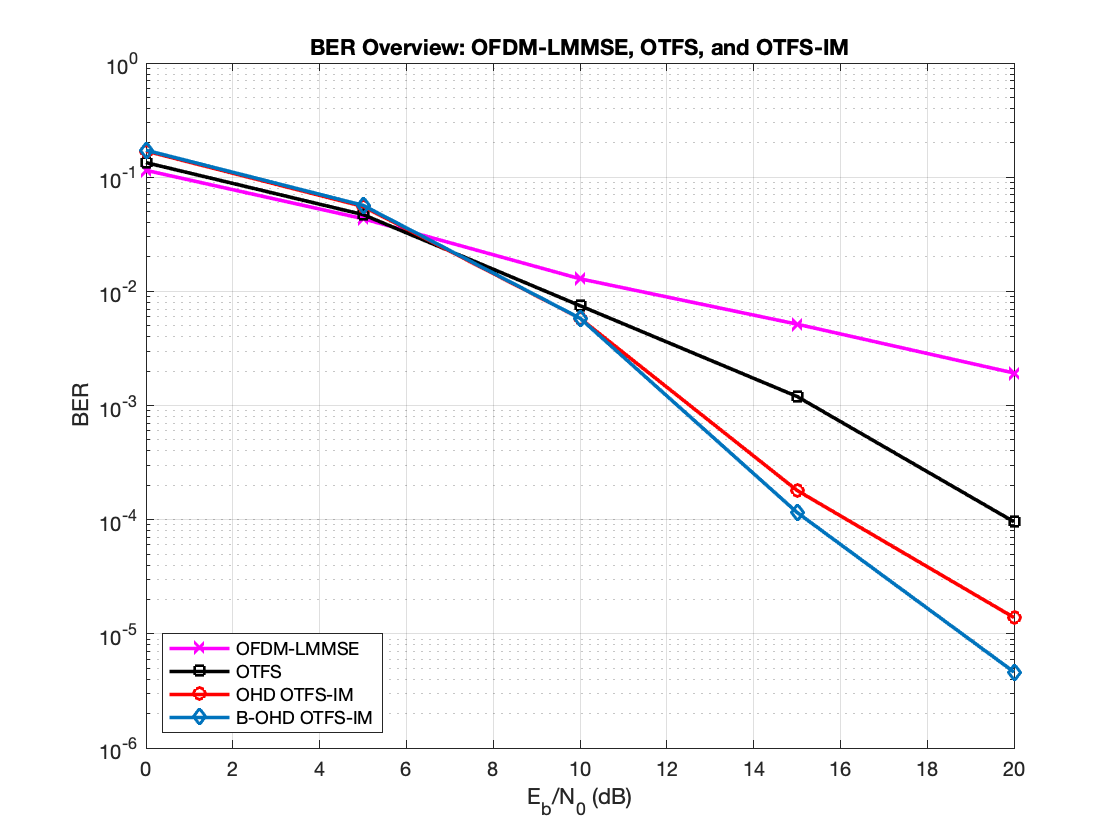
\includegraphics[width=0.88\linewidth]{Images/Chapter5/ber_overview_n5_k3.png}
    \caption{BER overview of OFDM-LMMSE, OTFS, and OTFS-IM for the \(n=5,k=3\) trade-off configuration}
    \label{fig:chapter5_ber_overview_n5_k3}
\end{figure}
}{%
\begin{figure}[H]
    \centering
    \fbox{\begin{minipage}[c][5cm][c]{0.86\linewidth}
        \centering
        Required figure file is missing:\\
        Images/Chapter5/ber\_overview\_n5\_k3.png
    \end{minipage}}
    \caption{BER overview of OFDM-LMMSE, OTFS, and OTFS-IM for the \(n=5,k=3\) trade-off configuration}
    \label{fig:chapter5_ber_overview_n5_k3}
\end{figure}
}

For \(n=5,k=3\), OHD and B-OHD no longer represent the same selected table. At \(10\) dB, both deterministic OTFS-IM schemes achieve approximately \(5.81\times10^{-3}\), which is lower than the baseline OTFS BER of approximately \(7.49\times10^{-3}\). At \(15\) dB, B-OHD becomes better than OHD, with a BER of about \(1.16\times10^{-4}\) compared with \(1.81\times10^{-4}\) for OHD. This behavior shows that the balancing criterion can change the high-SNR error trend, but the result must still be interpreted as a reliability-rate trade-off because \(\eta_{\mathrm{IM}}<\eta_{\mathrm{OTFS}}\). This configuration is therefore useful for pattern-selection analysis, while the \(n=6,k=5\) case remains the main rate-fair BER evidence.

Overall, this baseline comparison shows three important trends. First, OTFS-based transmission becomes more reliable than OFDM-LMMSE as the SNR increases under the considered delay-Doppler channel. Second, OTFS-IM can improve BER over baseline OTFS while maintaining the same spectral efficiency in the representative \(n=6,k=5\) case. Third, when the pattern table changes as in \(n=5,k=3\), OHD and B-OHD can produce different BER behavior, but the result must be interpreted together with spectral efficiency. For this reason, the next section focuses specifically on equal-spectral-efficiency OTFS-IM configurations before moving to pattern-level error analysis.


% !TEX root = ../../main.tex

\subsection{Equal Spectral Efficiency OTFS-IM Results}

The most important OTFS-IM results are obtained from configurations whose spectral efficiency is equal to that of the baseline OTFS system. In these cases, the comparison is not biased by a lower transmission rate. From Table~\ref{tab:chapter5_im_configurations}, the equal-SE configurations are \(n=4,k=3\), \(n=5,k=4\), and \(n=6,k=5\). All three cases satisfy
\begin{equation}
    \eta_{\mathrm{IM}} = 2.00~\mathrm{bits/symbol}
    =
    \eta_{\mathrm{OTFS}}.
    \label{eq:chapter5_equal_se_condition}
\end{equation}
Therefore, these configurations are used to evaluate whether OTFS-IM can improve the BER performance without sacrificing spectral efficiency.

Table~\ref{tab:chapter5_equal_se_ber_summary} summarizes the BER values of the equal-SE configurations at \(10\) dB and \(15\) dB. These two SNR points are more informative than the extreme high-SNR point because they avoid over-interpreting zero-error or near-zero-error outcomes caused by finite Monte Carlo simulation length.

\begin{table}[H]
    \centering
    \caption{BER summary of equal-SE OTFS-IM configurations}
    \label{tab:chapter5_equal_se_ber_summary}
    \begin{tabularx}{\linewidth}{>{\centering\arraybackslash}p{2.4cm}
                                  >{\centering\arraybackslash}p{1.6cm}
                                  >{\centering\arraybackslash}p{2.0cm}
                                  >{\centering\arraybackslash}p{2.2cm}
                                  >{\centering\arraybackslash}p{2.2cm}
                                  >{\Centering\arraybackslash}X}
        \toprule
        Configuration & \(E_b/N_0\) & OTFS BER & OHD OTFS-IM BER & B-OHD OTFS-IM BER & Interpretation \\
        \midrule
        \(4\)-\(3\) & 10 dB & \(7.49\times10^{-3}\) & \(6.71\times10^{-3}\) & \(6.71\times10^{-3}\) & Slight rate-fair gain \\
        \midrule
        \(4\)-\(3\) & 15 dB & \(1.20\times10^{-3}\) & \(2.20\times10^{-4}\) & \(2.20\times10^{-4}\) & Clear high-SNR gain \\
        \midrule
        \(5\)-\(4\) & 10 dB & \(7.49\times10^{-3}\) & \(6.64\times10^{-3}\) & \(6.64\times10^{-3}\) & Slight rate-fair gain \\
        \midrule
        \(5\)-\(4\) & 15 dB & \(1.20\times10^{-3}\) & \(3.20\times10^{-4}\) & \(3.20\times10^{-4}\) & Clear high-SNR gain \\
        \midrule
        \(6\)-\(5\) & 10 dB & \(7.49\times10^{-3}\) & \(6.41\times10^{-3}\) & \(6.41\times10^{-3}\) & Best 10 dB equal-SE case \\
        \midrule
        \(6\)-\(5\) & 15 dB & \(1.20\times10^{-3}\) & \(2.00\times10^{-4}\) & \(2.00\times10^{-4}\) & Strong equal-SE gain \\
        \bottomrule
    \end{tabularx}
\end{table}

The table shows a consistent trend. At \(10\) dB, all equal-SE OTFS-IM configurations improve slightly over baseline OTFS. The improvement is moderate because the receiver still needs to estimate both the active pattern and the active QAM symbols. At \(15\) dB, the improvement becomes more visible. In this SNR region, the noise level is low enough for the activation-pattern structure to contribute to more reliable detection.

Among the equal-SE configurations, \(n=6,k=5\) gives the best BER at both \(10\) dB and \(15\) dB in the deterministic OHD/B-OHD comparison. This is why it is used as the representative equal-SE case in Figure~\ref{fig:chapter5_ber_zoom_n6_k5}. The figure zooms into the \(5\)-\(20\) dB region and compares baseline OTFS with OHD and B-OHD OTFS-IM.

\IfFileExists{Images/Chapter5/ber_zoom_n6_k5.png}{%
\begin{figure}[H]
    \centering
    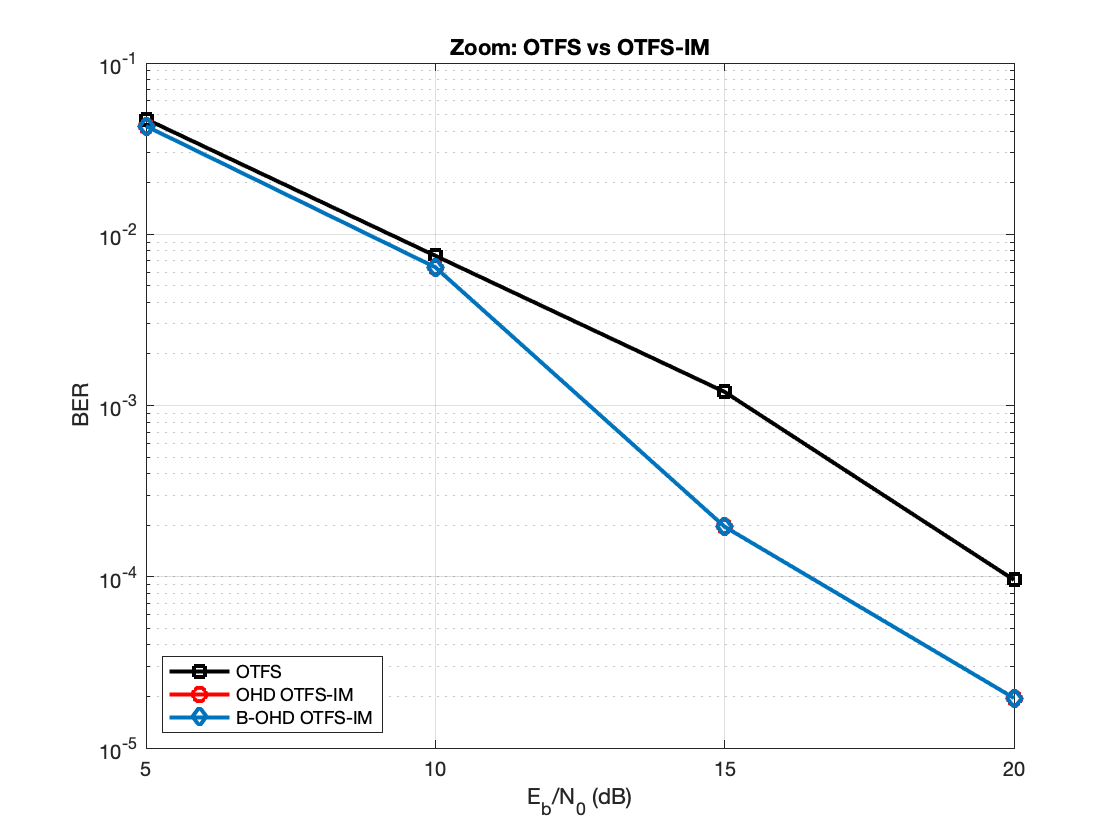
\includegraphics[width=0.88\linewidth]{Images/Chapter5/ber_zoom_n6_k5.png}
    \caption{BER zoom of baseline OTFS and equal-SE OTFS-IM for the \(n=6,k=5\) configuration}
    \label{fig:chapter5_ber_zoom_n6_k5}
\end{figure}
}{%
\begin{figure}[H]
    \centering
    \fbox{\begin{minipage}[c][5cm][c]{0.86\linewidth}
        \centering
        Required figure file is missing:\\
        Images/Chapter5/ber\_zoom\_n6\_k5.png
    \end{minipage}}
    \caption{BER zoom of baseline OTFS and equal-SE OTFS-IM for the \(n=6,k=5\) configuration}
    \label{fig:chapter5_ber_zoom_n6_k5}
\end{figure}
}

Figure~\ref{fig:chapter5_ber_zoom_n6_k5} confirms that the OTFS-IM curves become lower than the baseline OTFS curve from the medium-SNR region onward. At \(5\) dB, the schemes are close because detection is still noise-limited. At \(10\) dB and above, the index-modulated structure begins to provide a measurable BER reduction. Since the spectral efficiency is unchanged, this result is stronger than a lower-rate BER gain.

Another important observation is that OHD and B-OHD overlap in all three equal-SE configurations listed in Table~\ref{tab:chapter5_equal_se_ber_summary}. This does not indicate a plotting error. For \(n=4,k=3\), the number of valid activation patterns is \(\binom{4}{3}=4\), and the number of index-addressable patterns is also four. Therefore, all valid patterns are selected, leaving no additional freedom for B-OHD to improve the table. For \(n=5,k=4\) and \(n=6,k=5\), the valid pattern sets are also highly constrained, so the OHD and B-OHD selection criteria lead to the same effective pattern table.

This result clarifies the role of B-OHD in the thesis. B-OHD is not expected to improve every configuration. Its advantage can only appear when there is enough freedom to choose among multiple candidate pattern sets with the same minimum Hamming distance. In equal-SE configurations with a small or constrained pattern space, OHD and B-OHD may naturally become identical. This is why the \(n=5,k=3\) configuration is later used for pattern-selection validation, while the equal-SE configurations are used mainly to prove that OTFS-IM can improve BER without reducing spectral efficiency.

In summary, the equal-SE results provide the most important evidence for the usefulness of OTFS-IM in this thesis. Across \(4\)-\(3\), \(5\)-\(4\), and \(6\)-\(5\), OTFS-IM maintains the same spectral efficiency as baseline OTFS and still obtains lower BER in the medium and high SNR regions. The improvement is not uniform at all SNR values, but the trend is consistent enough to justify a deeper error-decomposition analysis in the next section.


% !TEX root = ../../main.tex

\subsection{OTFS-IM Error Decomposition}

The BER curves in the previous sections show the final end-to-end performance of OTFS-IM. However, total BER alone does not explain where the errors are produced inside the index-modulated receiver. In OTFS-IM, a detected bit can be wrong because the receiver selects an incorrect active-position pattern, because it detects an incorrect QAM symbol on an active position, or because both events occur in the same IM block. Therefore, this section decomposes the OTFS-IM result into index BER, symbol BER, and pattern error rate.

The decomposition is especially useful for interpreting whether the performance of a pattern-selection method is limited by the geometry of the selected activation patterns or by the reliability of the symbol decisions after the active positions have already been estimated. In the simulation, the index BER is computed from the recovered pattern bits, the symbol BER is computed from the recovered QAM bits on the active positions, and the pattern error rate measures the probability that the active-position pattern of an IM block is detected incorrectly.

\IfFileExists{Images/Chapter5/error_decomposition_n6_k5.png}{%
\begin{figure}[H]
    \centering
    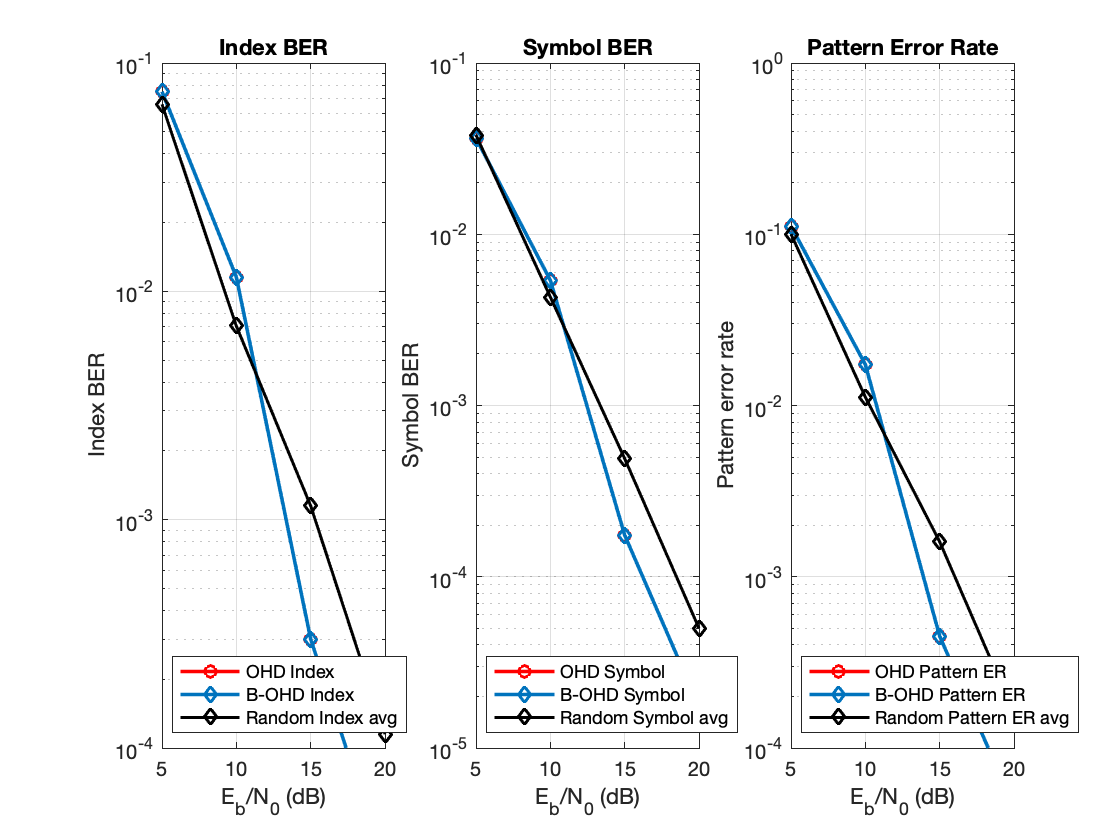
\includegraphics[width=0.95\linewidth]{Images/Chapter5/error_decomposition_n6_k5.png}
    \caption{Error decomposition of OHD and B-OHD OTFS-IM for \(n=6,k=5\)}
    \label{fig:chapter5_error_decomposition_n6_k5}
\end{figure}
}{%
\begin{figure}[H]
    \centering
    \fbox{%
        \begin{minipage}[c][0.25\textheight][c]{0.88\linewidth}
            \centering
            Required figure file is missing:\\
            Images/Chapter5/error\_decomposition\_n6\_k5.png
        \end{minipage}
    }
    \caption{Error decomposition of OHD and B-OHD OTFS-IM for \(n=6,k=5\)}
    \label{fig:chapter5_error_decomposition_n6_k5}
\end{figure}
}

Figure~\ref{fig:chapter5_error_decomposition_n6_k5} presents the error decomposition for the equal-spectral-efficiency configuration \(n=6,k=5\). This configuration is selected because it was used as the main equal-SE case in the previous section, where OTFS-IM and baseline OTFS both transmit \(2.00\) bits per resource element. As a result, the decomposition can be interpreted without the ambiguity of a rate advantage or a rate penalty.

At low SNR, both the index and symbol components are relatively large. This behavior is expected because the MP detector receives unreliable soft information from the delay-Doppler grid. Under this condition, the receiver may confuse the active positions and may also assign incorrect QAM symbols to positions that are detected as active. Therefore, the BER of OTFS-IM is not yet clearly separated into a purely index-limited or purely symbol-limited regime.

At medium SNR, the decomposition becomes more informative. For the \(n=6,k=5\) case, the OHD and B-OHD pattern tables are identical in the implemented simulation, so the two curves overlap. At \(E_b/N_0=10~\mathrm{dB}\), the total BER is approximately \(6.41\times10^{-3}\), while the measured index BER and symbol BER are approximately \(1.16\times10^{-2}\) and \(5.39\times10^{-3}\), respectively. In the bit-level contribution reported by the simulation, the symbol component accounts for about \(70\%\) of the total erroneous bits and the index component accounts for about \(30\%\). This means that, although pattern detection is important, the final BER is also strongly affected by the reliability of QAM symbol decisions on the detected active positions.

The pattern error rate provides a complementary view. At \(10~\mathrm{dB}\), the pattern error rate is approximately \(1.74\times10^{-2}\), which is higher than the total BER because one wrong pattern event is counted at the block level rather than at the bit level. A single pattern error does not necessarily imply that all bits in the IM block are wrong. Some symbol bits may still be recovered correctly, and some wrong active-position decisions may affect only part of the index-bit representation. For this reason, pattern error rate should not be compared directly with total BER as if they were the same metric. It is better interpreted as a diagnostic indicator of active-position reliability.

At higher SNR, the index and symbol components both decrease sharply. In the reported \(n=6,k=5\) result, the OTFS-IM BER approaches the Monte Carlo resolution at \(20~\mathrm{dB}\), and both index and symbol BER become nearly zero. This confirms that the detector is able to exploit the delay-Doppler representation effectively when the noise level is sufficiently low. It also shows that the performance gain observed in the BER curves is not produced by only one part of the receiver. Instead, it comes from the combined improvement in active-pattern detection and active-symbol detection.

The main conclusion from this decomposition is that OTFS-IM performance is jointly limited by pattern reliability and symbol reliability. Pattern selection can reduce the probability of confusing activation patterns, but it cannot fully determine the BER by itself. Once the active pattern is detected with reasonable reliability, the remaining errors are increasingly dominated by the QAM decisions on the active positions. This observation is important for the following section, where deterministic pattern selection is compared with random pattern selection. A good pattern table is beneficial, but its advantage is configuration-dependent and must be evaluated together with the detector behavior and the operating SNR range.


% !TEX root = ../../main.tex

\subsection{Pattern Selection Validation}

The previous sections evaluated OTFS-IM as an end-to-end transmission scheme. This section focuses on the pattern-selection component itself. In the proposed OTFS-IM transmitter, only a subset of all possible activation patterns is used for mapping the index bits. The purpose of OHD and B-OHD selection is to choose this subset more carefully than a purely arbitrary pattern table. The validation therefore compares deterministic pattern selection with a random-pattern diagnostic baseline.

The configuration \(n=5,k=3\) is used as the main validation case because it provides a non-trivial pattern-selection problem while keeping the exact OHD search feasible. For this configuration, there are \(\binom{5}{3}=10\) possible constant-weight activation patterns, and the system selects \(2^{b_1}=8\) patterns for index-bit mapping. Hence, OHD and B-OHD are forced to discard some candidate patterns, but the candidate set is still small enough to allow an exact comparison. This makes the configuration suitable for explaining the effect of pattern geometry without making the pattern-selection result visually or computationally excessive.

\IfFileExists{Images/Chapter5/pattern_geometry_n5_k3.png}{%
\begin{figure}[H]
    \centering
    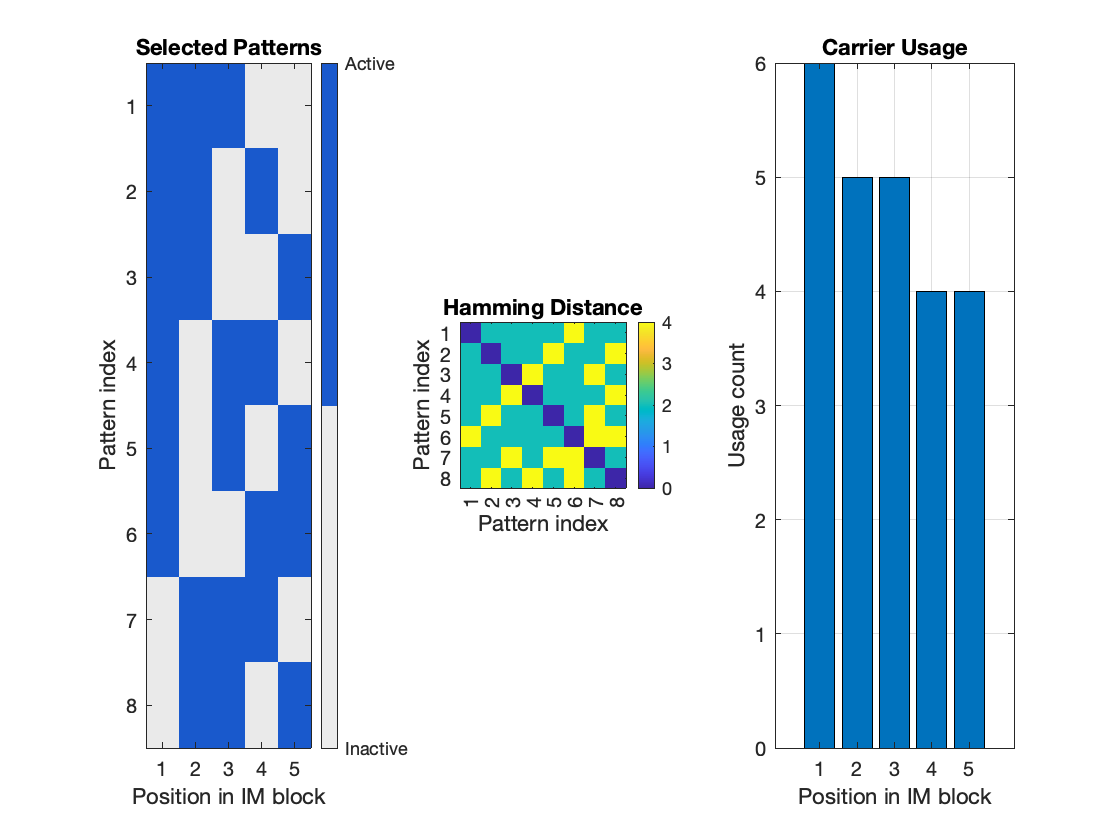
\includegraphics[width=0.92\linewidth]{Images/Chapter5/pattern_geometry_n5_k3.png}
    \caption{Selected pattern geometry for OHD-based OTFS-IM with \(n=5,k=3\)}
    \label{fig:chapter5_pattern_geometry_n5_k3}
\end{figure}
}{%
\begin{figure}[H]
    \centering
    \fbox{%
        \begin{minipage}[c][0.25\textheight][c]{0.88\linewidth}
            \centering
            Required figure file is missing:\\
            Images/Chapter5/pattern\_geometry\_n5\_k3.png
        \end{minipage}
    }
    \caption{Selected pattern geometry for OHD-based OTFS-IM with \(n=5,k=3\)}
    \label{fig:chapter5_pattern_geometry_n5_k3}
\end{figure}
}

Figure~\ref{fig:chapter5_pattern_geometry_n5_k3} illustrates the selected activation patterns and their geometric properties. The selected-pattern map shows which positions are active in each IM block. The Hamming-distance map indicates how different the selected patterns are from each other, while the carrier-usage plot shows whether the active positions are distributed evenly across the block. These three views are useful because pattern selection in OTFS-IM is not only about maximizing pairwise distance. A pattern table with good distance but unbalanced carrier usage may still create unequal position reliability.

For the \(n=5,k=3\) configuration, the spectral efficiency is
\begin{equation}
    \eta_{\mathrm{IM}}
    =
    \frac{\left\lfloor \log_2 \binom{5}{3} \right\rfloor + 3\log_2 4}{5}
    =
    \frac{3+6}{5}
    =
    1.80~\text{bits/symbol}.
    \label{eq:chapter5_se_53_validation}
\end{equation}
This rate is lower than the baseline OTFS rate of \(2.00~\text{bits/symbol}\), so this configuration should be interpreted as a reliability-oriented OTFS-IM setting rather than a strict equal-SE comparison. The BER improvement obtained in this case therefore represents a BER-SE trade-off: the system sacrifices \(10\%\) spectral efficiency to improve reliability in the medium-to-high-SNR region.

The geometry result also explains the difference between OHD and B-OHD. With OHD, the selected pattern table has carrier usage \([6,5,5,4,4]\), which indicates that the first position is activated more often than the last two positions. B-OHD preserves the same minimum Hamming distance but improves the usage balance to approximately \([5,4,5,5,5]\). This does not change the basic OTFS-IM structure, but it makes the selected pattern table less biased toward a small number of positions. Such balancing is expected to be more useful when the detector output is already reliable enough for the remaining pattern-geometry differences to matter.

\IfFileExists{Images/Chapter5/pattern_validation_n5_k3.png}{%
\begin{figure}[H]
    \centering
    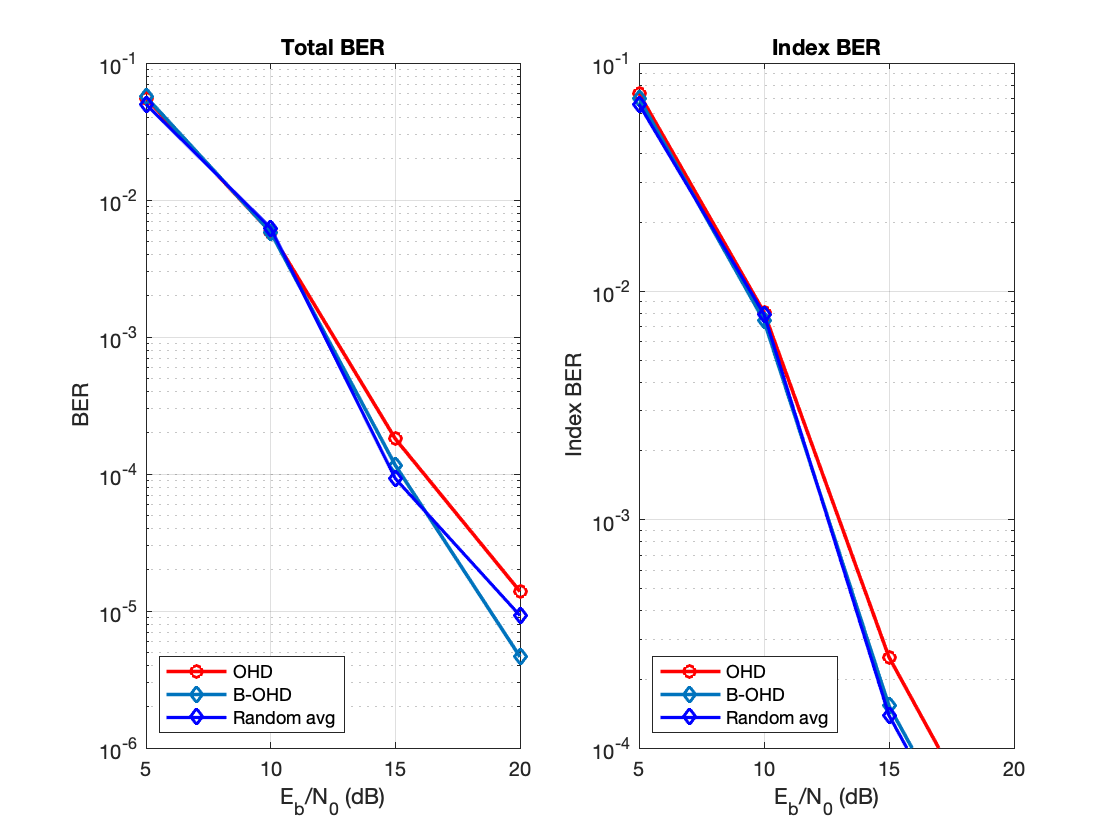
\includegraphics[width=0.95\linewidth]{Images/Chapter5/pattern_validation_n5_k3.png}
    \caption{Validation of OHD and B-OHD pattern selection against random pattern tables for \(n=5,k=3\)}
    \label{fig:chapter5_pattern_validation_n5_k3}
\end{figure}
}{%
\begin{figure}[H]
    \centering
    \fbox{%
        \begin{minipage}[c][0.28\textheight][c]{0.88\linewidth}
            \centering
            Required figure file is missing:\\
            Images/Chapter5/pattern\_validation\_n5\_k3.png
        \end{minipage}
    }
    \caption{Validation of OHD and B-OHD pattern selection against random pattern tables for \(n=5,k=3\)}
    \label{fig:chapter5_pattern_validation_n5_k3}
\end{figure}
}

Figure~\ref{fig:chapter5_pattern_validation_n5_k3} compares OHD, B-OHD, and the random-pattern average. The random curve is not used as a proposed design method in this thesis. Instead, it is used as a diagnostic reference to check whether the deterministic selection rules provide a meaningful advantage over arbitrary pattern choices. This comparison is necessary because a random pattern table can sometimes have favorable distance or usage properties, especially when the candidate set is small.

At \(10~\mathrm{dB}\), the total BER values are approximately \(5.81\times10^{-3}\), \(5.81\times10^{-3}\), and \(6.24\times10^{-3}\) for OHD, B-OHD, and random selection, respectively. At this SNR point, deterministic pattern selection provides a modest but visible improvement over the random average. The index BER values are also close: \(8.10\times10^{-3}\) for OHD, \(7.43\times10^{-3}\) for B-OHD, and \(7.94\times10^{-3}\) for the random average. This indicates that B-OHD slightly improves the index reliability compared with OHD while remaining competitive with the random baseline.

At \(15~\mathrm{dB}\), the performance difference becomes more visible in the total BER. OHD reaches approximately \(1.81\times10^{-4}\), B-OHD reaches \(1.16\times10^{-4}\), and the random average reaches \(9.0\times10^{-5}\). The random average is slightly lower at this point, but B-OHD still improves over the original OHD table. This result should not be interpreted as a failure of deterministic pattern selection. Rather, it shows that random pattern tables can occasionally be strong, and that the proposed deterministic design should be evaluated against them instead of only against the OTFS baseline.

The pattern error rate provides an additional explanation. At \(10~\mathrm{dB}\), the pattern error rates are approximately \(1.47\times10^{-2}\), \(1.36\times10^{-2}\), and \(1.49\times10^{-2}\) for OHD, B-OHD, and random selection, respectively. B-OHD gives the lowest pattern error rate in this region, which is consistent with its improved carrier-usage balance. At \(15~\mathrm{dB}\), all three methods have very small pattern error rates, and the remaining BER differences become sensitive to both symbol decisions and Monte Carlo variation.

Overall, the \(n=5,k=3\) validation gives a clearer pattern-selection story than configurations where OHD and B-OHD overlap. OHD provides a structured pattern table based on Hamming-distance separation, while B-OHD improves the balance of the selected table without changing the OTFS-IM receiver. The results show that B-OHD can improve OHD, especially in the medium-to-high-SNR region. At the same time, the random baseline remains important because it shows that pattern selection is configuration-dependent and that Hamming distance alone does not guarantee universal superiority. This observation motivates future channel-aware or detector-aware pattern selection methods, while still supporting the use of structured pattern design in the present OTFS-IM system.


% !TEX root = ../../main.tex

\subsection{BER-SE Trade-Off Across Configurations}

The previous sections examined representative OTFS-IM configurations in detail. This section combines the available simulation results into a configuration-level comparison. The purpose is not only to identify the lowest BER curve, but also to interpret each result together with its spectral efficiency. This distinction is important because an OTFS-IM configuration may improve BER by reducing the number of transmitted information bits per block, while another configuration may preserve the same spectral efficiency as the baseline OTFS system.

Two summary figures are used for this comparison. The first figure compares the BER values of different OTFS-IM configurations at selected SNR points. This view is useful for quickly identifying which configurations operate below the OTFS reference curve. The second figure places the same BER values against spectral efficiency. This view clarifies whether a BER improvement is obtained at equal spectral efficiency or by accepting a lower-rate transmission mode.

\IfFileExists{Images/Chapter5/configuration_ber_summary.png}{%
\begin{figure}[H]
    \centering
    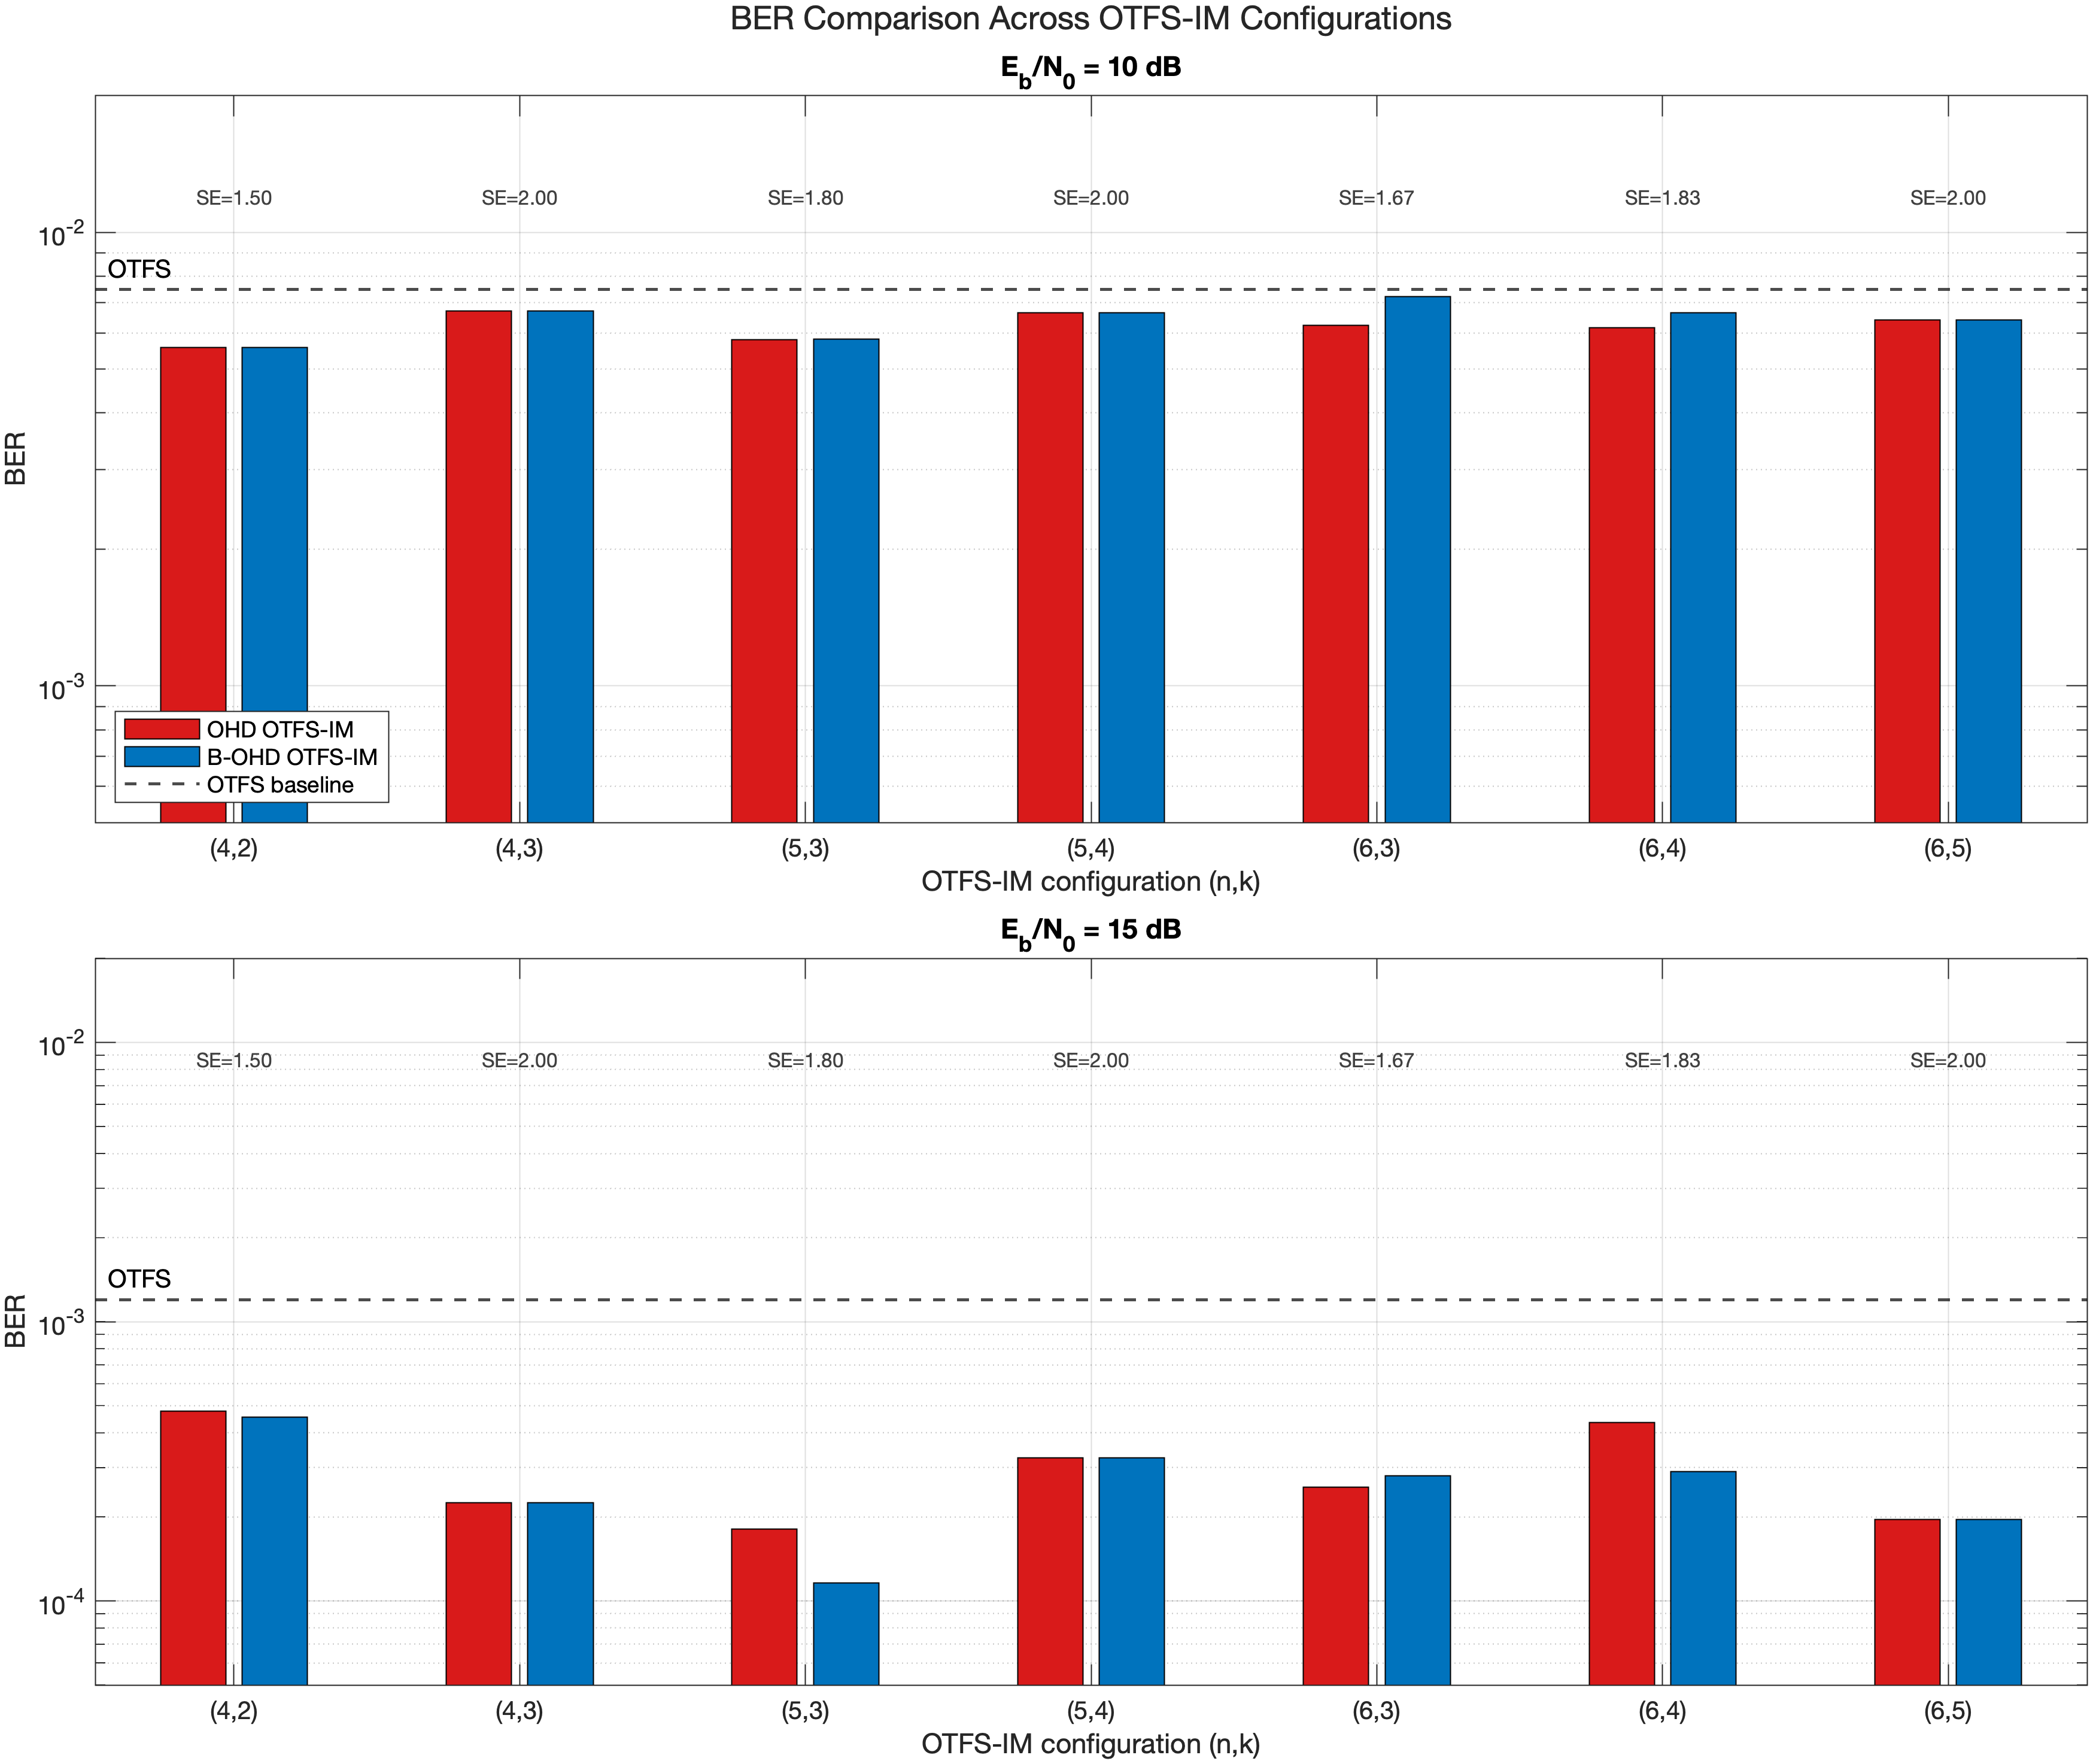
\includegraphics[width=0.95\linewidth]{Images/Chapter5/configuration_ber_summary.png}
    \caption{Configuration-level BER comparison for OHD and B-OHD OTFS-IM at selected SNR points}
    \label{fig:chapter5_configuration_ber_summary}
\end{figure}
}{%
\begin{figure}[H]
    \centering
    \fbox{%
        \begin{minipage}[c][0.28\textheight][c]{0.88\linewidth}
            \centering
            Required figure file is missing:\\
            Images/Chapter5/configuration\_ber\_summary.png
        \end{minipage}
    }
    \caption{Configuration-level BER comparison for OHD and B-OHD OTFS-IM at selected SNR points}
    \label{fig:chapter5_configuration_ber_summary}
\end{figure}
}

Figure~\ref{fig:chapter5_configuration_ber_summary} summarizes the BER of the simulated OTFS-IM configurations at \(E_b/N_0=10~\mathrm{dB}\) and \(E_b/N_0=15~\mathrm{dB}\). The dashed horizontal line represents the baseline OTFS BER at the same SNR value. Therefore, a bar below this line indicates that the corresponding OTFS-IM configuration achieves a lower BER than baseline OTFS at that operating point.

At \(10~\mathrm{dB}\), most OTFS-IM configurations are already below the OTFS baseline. However, the separation is moderate because the detector still operates in a region where both index errors and symbol errors contribute to the total BER. In this region, changing the pattern table from OHD to B-OHD does not always create a large visible gain. This behavior is consistent with the error-decomposition results: when the received reliability is still limited, the total BER is dominated not only by the geometric distance between activation patterns, but also by the quality of the MP detector output.

At \(15~\mathrm{dB}\), the difference between configurations becomes clearer. Several OTFS-IM configurations move further below the OTFS baseline, showing that index modulation can be beneficial in the medium-to-high-SNR region. The \(n=5,k=3\) case is particularly useful for pattern-selection validation because B-OHD improves over OHD while keeping the same IM block size and modulation order. This confirms that the balancing term in B-OHD can be meaningful when the selected pattern table is not identical to the OHD table. By contrast, in configurations such as \(n=6,k=5\), OHD and B-OHD may select effectively the same pattern table, so their BER curves overlap.

\IfFileExists{Images/Chapter5/ber_se_tradeoff.png}{%
\begin{figure}[H]
    \centering
    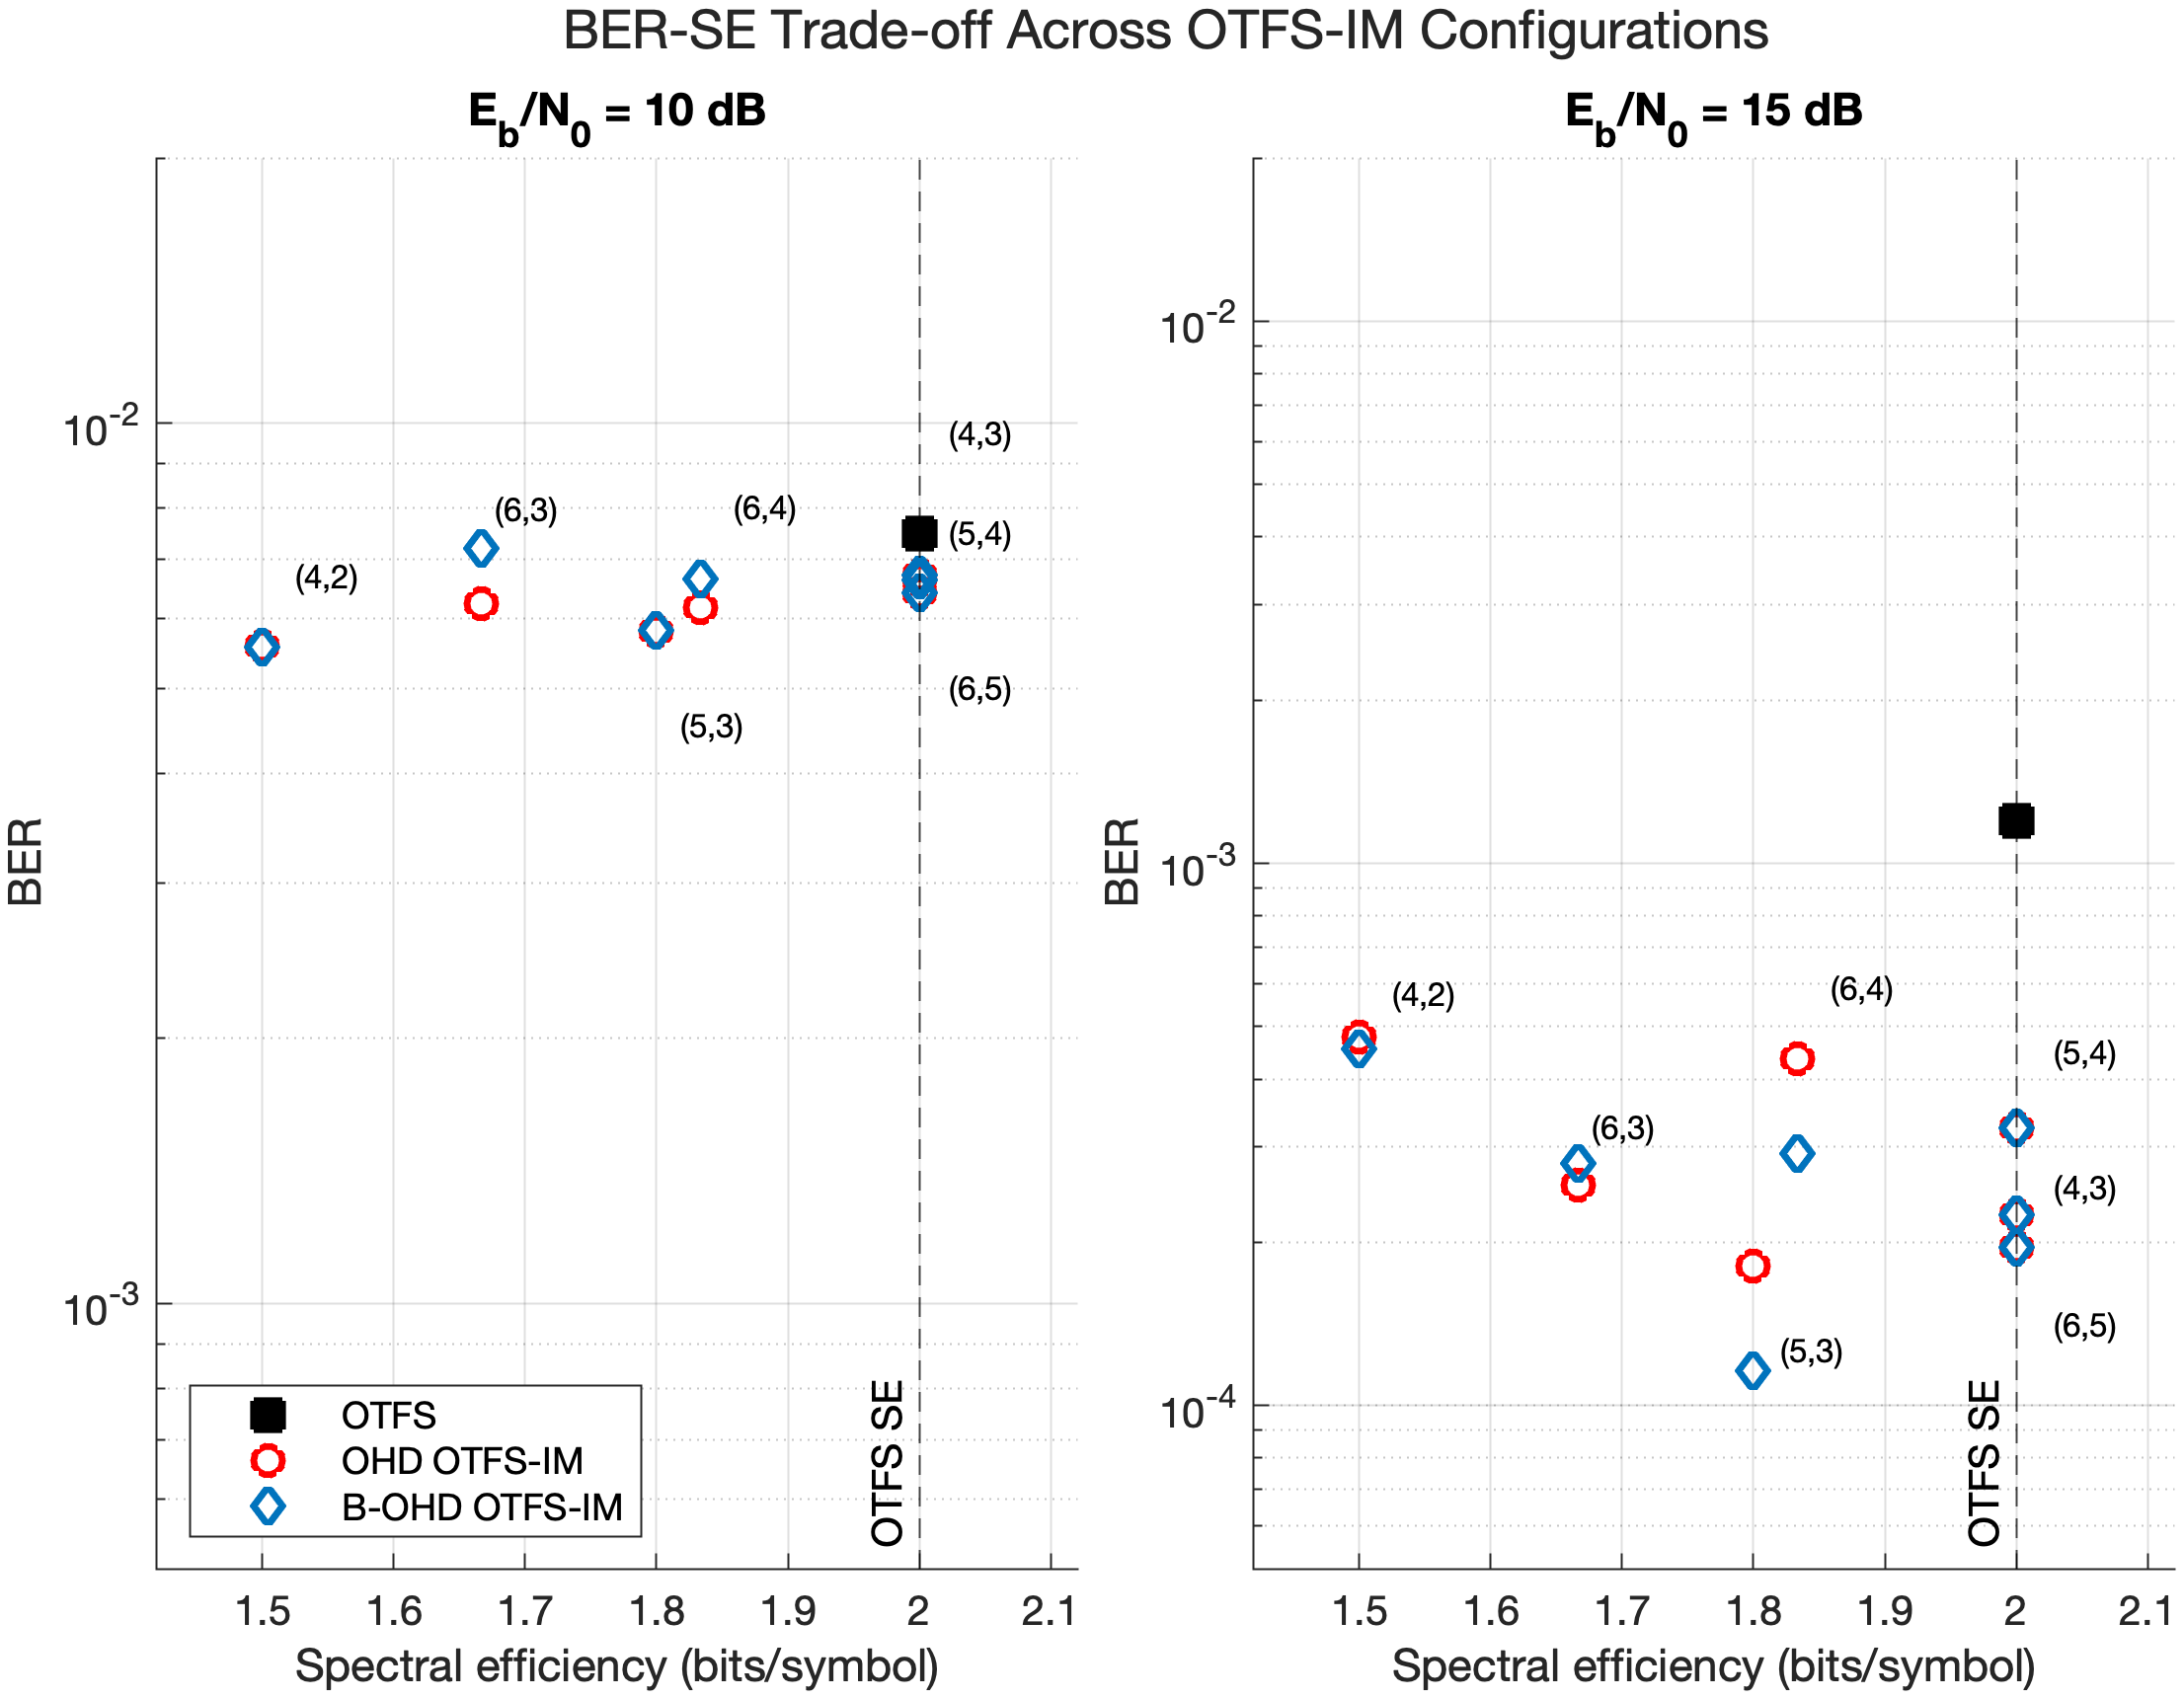
\includegraphics[width=0.95\linewidth]{Images/Chapter5/ber_se_tradeoff.png}
    \caption{BER-SE trade-off across OTFS-IM configurations at selected SNR points}
    \label{fig:chapter5_ber_se_tradeoff}
\end{figure}
}{%
\begin{figure}[H]
    \centering
    \fbox{%
        \begin{minipage}[c][0.28\textheight][c]{0.88\linewidth}
            \centering
            Required figure file is missing:\\
            Images/Chapter5/ber\_se\_tradeoff.png
        \end{minipage}
    }
    \caption{BER-SE trade-off across OTFS-IM configurations at selected SNR points}
    \label{fig:chapter5_ber_se_tradeoff}
\end{figure}
}

Figure~\ref{fig:chapter5_ber_se_tradeoff} gives a more complete interpretation of the same results. The vertical dashed line marks the spectral efficiency of the baseline OTFS system, which is \(2.00~\text{bits/symbol}\) for 4-QAM. Points located on this line correspond to equal-SE OTFS-IM configurations, while points to the left correspond to lower-SE configurations. This representation is important because a lower BER at a smaller spectral efficiency should not be interpreted in the same way as a lower BER at equal spectral efficiency.

The equal-SE configurations, including \(n=4,k=3\), \(n=5,k=4\), and \(n=6,k=5\), are the most direct comparison against baseline OTFS. These cases show that OTFS-IM can preserve the same nominal spectral efficiency while improving BER in the simulated delay-Doppler channel. Among them, the \(n=6,k=5\) configuration is the main equal-SE example used in this chapter because it has a larger IM block and provides clearer high-SNR performance separation from baseline OTFS. However, the overlap between OHD and B-OHD in this case also shows that the proposed balancing criterion does not always change the selected pattern table.

The lower-SE configurations, such as \(n=4,k=2\), \(n=5,k=3\), \(n=6,k=3\), and \(n=6,k=4\), occupy the left side of the trade-off plot. Their BER values are generally competitive because they transmit fewer information bits per block. These configurations are useful when reliability is prioritized over throughput, but their gains must be described as BER-SE trade-offs rather than pure improvements over baseline OTFS. In particular, the \(n=5,k=3\) case is valuable because it demonstrates the difference between OHD and B-OHD in a setting where exact pattern selection remains feasible and the pattern table is not trivially identical.

The comparison also shows that B-OHD should be interpreted as a refinement of OHD rather than a universally dominant detector or modulation method. B-OHD does not change the OTFS-IM signal model, the MP detector, or the modulation order. It only changes the selected activation-pattern table by adding a carrier-usage balancing criterion. Therefore, its gain appears mainly when the selected table has room for improvement in usage balance and when the detector output is reliable enough for such pattern-level differences to affect the final decision.

Overall, the BER-SE summary supports three design insights. First, OTFS-IM can outperform baseline OTFS in the simulated high-Doppler delay-Doppler channel, especially from the medium-SNR region onward. Second, equal-SE configurations are the strongest evidence that OTFS-IM is not merely improving BER by lowering the information rate. Third, pattern selection remains configuration-dependent: B-OHD can improve OHD when the OHD table is unbalanced, but random or structurally similar tables can sometimes perform competitively. For this reason, the final evaluation should report both the absolute BER curves and the BER-SE trade-off, rather than relying on a single BER plot.


% !TEX root = ../../main.tex

\subsection{Design Insights and Chapter Summary}

This chapter evaluated the baseline OFDM-LMMSE, baseline OTFS, and OTFS-IM systems under the same delay-Doppler channel and modulation assumptions. The results show that OTFS-IM is not simply an additional mapping layer placed on top of OTFS. Its performance depends jointly on the IM block size, the number of active positions, the spectral efficiency, the selected activation-pattern table, and the reliability of the detector output. Therefore, the most meaningful conclusion is obtained by reading the BER curves together with the error-decomposition and BER-SE trade-off results.

The first important observation is that OTFS-IM can improve BER over baseline OTFS in the simulated high-Doppler delay-Doppler channel. This is most clearly shown in the medium-to-high-SNR region, where the detector output becomes reliable enough for the activation pattern and symbol decisions to separate more cleanly. In the equal-spectral-efficiency cases, especially \(n=6,k=5\), OTFS-IM preserves the same nominal rate as baseline OTFS while reducing BER. This is the strongest result in the chapter because it shows that the gain does not only come from lowering the number of transmitted information bits.

At low SNR, the advantage of OTFS-IM is less consistent. In this region, the received samples are strongly affected by noise, and the MP detector has difficulty distinguishing both the active positions and the transmitted QAM symbols. As a result, the total BER is influenced more by detector uncertainty than by the exact geometry of the selected pattern table. This explains why OHD, B-OHD, and random selection can be close to each other at some SNR points. It also explains why pattern selection alone cannot be expected to solve all low-SNR errors.

The error-decomposition results provide a more detailed view of the OTFS-IM error mechanism. The total BER is produced by two different sources: index-bit errors and symbol-bit errors. Index errors occur when the receiver selects the wrong active-position pattern, while symbol errors occur when the active positions are detected but the QAM symbols are decoded incorrectly. In the simulated results, symbol errors remain a major contribution to the total BER, especially at moderate SNR. This means that improving pattern geometry is useful, but it should be combined with reliable detection and symbol estimation. A pattern table with good Hamming-distance properties cannot fully compensate for poor detector reliability.

The comparison between OHD and B-OHD gives a more careful interpretation of the proposed pattern-selection improvement. OHD selects activation patterns by prioritizing Hamming-distance separation. B-OHD keeps this idea but additionally considers carrier-usage balance. This makes B-OHD a refinement of OHD rather than a different receiver or a different modulation scheme. The gain of B-OHD appears when the OHD table is unbalanced and when the selected table can be modified without reducing the minimum Hamming distance. The \(n=5,k=3\) configuration illustrates this behavior because B-OHD improves the usage distribution and provides better performance than OHD at the selected operating points.

However, B-OHD does not always produce a different pattern table. In configurations such as \(n=6,k=5\), the selected OHD and B-OHD tables can become effectively identical, leading to overlapping BER curves. This is not a simulation error. It means that the OHD solution is already balanced enough under that configuration, or that the available candidate patterns do not allow B-OHD to produce a meaningfully different table. This result is useful because it prevents an overclaimed conclusion: B-OHD is beneficial when the pattern-selection problem has room for balancing, but it is not universally superior in every \((n,k)\) setting.

The random-pattern baseline also plays an important role in the evaluation. It shows whether a deterministic pattern-selection rule is truly useful or whether similar performance could be obtained from an arbitrary pattern table. In some cases, the random average is competitive with OHD or B-OHD, particularly when the number of candidate patterns is small or when several pattern tables have similar distance properties. Therefore, the random baseline should not be removed from the analysis. Its presence makes the evaluation more honest and strengthens the conclusion that pattern selection is configuration-dependent.

The BER-SE trade-off analysis further clarifies how the configurations should be interpreted. Equal-SE configurations such as \(n=4,k=3\), \(n=5,k=4\), and \(n=6,k=5\) provide the fairest direct comparison with baseline OTFS because they preserve the same spectral efficiency of \(2.00~\text{bits/symbol}\). Lower-SE configurations, such as \(n=4,k=2\), \(n=5,k=3\), \(n=6,k=3\), and \(n=6,k=4\), may achieve lower BER, but part of that improvement comes from transmitting fewer information bits per IM block. These lower-SE configurations are still useful because practical communication systems may choose reliability over rate in difficult channel conditions, but their results should be described as a rate-reliability trade-off rather than a strict performance gain at equal rate.

From a design perspective, the simulation results suggest that the choice of \((n,k)\) should not be made only from the spectral-efficiency formula. A larger \(k\) can help preserve rate, while a smaller \(k\) may improve reliability by reducing the number of active symbols and changing the pattern-detection problem. At the same time, increasing \(n\) enlarges the pattern space and can make exact pattern selection more expensive. Therefore, the final OTFS-IM design must balance spectral efficiency, BER performance, pattern-selection complexity, and detector reliability.

The results also reveal several limitations of the present simulation framework. First, the channel is modeled in the delay-Doppler domain with discrete delay and Doppler taps, but the simulation does not sweep a physical velocity parameter. Therefore, the results support the evaluation of a high-Doppler or doubly selective channel model, while a separate velocity-based study would be needed to quantify performance at specific speeds such as vehicular, railway, or UAV scenarios. Second, the Monte Carlo simulation uses a finite number of frames, so very low BER points may still contain statistical variation. Third, the receiver uses the same general MP detection principle for the compared OTFS-IM designs; more advanced channel-aware, detector-aware, or soft-output detection methods may further change the relative performance.

In summary, this chapter confirms that OTFS-IM is a meaningful extension of baseline OTFS for delay-Doppler-domain transmission. The simulations show that OTFS-IM can improve BER, including in equal-SE cases, and that pattern-table design affects the reliability of index detection. The proposed B-OHD method improves OHD when carrier-usage balancing changes the selected pattern table, but its gain is configuration-dependent. These findings provide the basis for the final conclusion of the thesis: OTFS-IM offers a flexible BER-SE design space for high-mobility-oriented wireless channels, and structured pattern selection is a useful but not standalone component of that design.


\newpage

\section*{CHAPTER 6. CONCLUSION AND FUTURE WORK}
\addcontentsline{toc}{section}{CHAPTER 6. CONCLUSION AND FUTURE WORK}

% =========================================================
% Numbering for Chapter 6
% =========================================================
\setcounter{section}{6}
\setcounter{subsection}{0}
\setcounter{subsubsection}{0}
\setcounter{figure}{0}
\setcounter{table}{0}
\setcounter{equation}{0}

\renewcommand{\thefigure}{6.\arabic{figure}}
\renewcommand{\thetable}{6.\arabic{table}}
\renewcommand{\theequation}{6.\arabic{equation}}
\renewcommand{\theHfigure}{6.\arabic{figure}}
\renewcommand{\theHtable}{6.\arabic{table}}
\renewcommand{\theHequation}{6.\arabic{equation}}

% =========================================================
% Chapter Introduction
% =========================================================
This chapter concludes the thesis by summarizing the main contributions, key simulation findings, remaining limitations, and possible future extensions. The work has focused on the design and performance evaluation of OTFS with index modulation for high-mobility-oriented delay-Doppler channels, with particular attention to BER performance, spectral-efficiency trade-offs, and activation-pattern selection.

% =========================================================
% Chapter Sections
% =========================================================
\subsection{Main Contributions}

The first contribution of this thesis is the construction of a complete baseline OTFS simulation framework. The system includes delay-Doppler-domain symbol placement, OTFS modulation and demodulation, a discrete delay-Doppler channel model with multipath delay and Doppler taps, AWGN addition, and MP-based detection. This framework provides the reference system used to evaluate the behavior of OTFS under a doubly selective channel and also serves as the foundation for the OTFS-IM extension.

The second contribution is the implementation of an OTFS-IM transmission and reception structure. Instead of activating all delay-Doppler resource elements as in conventional OTFS, the OTFS-IM system divides the grid into IM blocks and transmits information through both QAM symbols and active-position indices. This design makes it possible to study how index modulation changes the BER behavior and spectral-efficiency trade-off of the baseline OTFS system.

The third contribution is the integration of structured activation-pattern selection into the OTFS-IM system. The OHD method is used to select pattern tables with large Hamming-distance separation between activation patterns, while the proposed B-OHD refinement additionally considers carrier-usage balance. This allows the thesis to evaluate not only whether OTFS-IM improves over OTFS, but also whether the geometry of the selected activation patterns affects index detection reliability.

The fourth contribution is the inclusion of a random-pattern validation baseline. Random pattern selection is not treated as the proposed method, but as a diagnostic reference. By comparing OHD and B-OHD with random pattern tables, the thesis avoids relying only on idealized deterministic selection and provides a more honest evaluation of whether structured pattern design gives a meaningful advantage.

The final contribution is the simulation-based performance analysis across multiple OTFS-IM configurations. The evaluation considers total BER, index BER, symbol BER, pattern error rate, and BER-SE trade-off. This makes the analysis deeper than a single BER comparison because it separates equal-spectral-efficiency gains from rate-reliability trade-offs and explains when B-OHD improves OHD and when both methods become effectively identical.

\begin{table}[htbp]
    \centering
    \footnotesize
    \caption{Summary of thesis contributions and possible extensions}
    \label{tab:chapter6_contribution_summary}
    \renewcommand{\arraystretch}{1.22}
    \setlength{\tabcolsep}{4pt}
    \begin{tabularx}{\linewidth}{>{\RaggedRight\arraybackslash}p{0.16\linewidth}
    >{\RaggedRight\arraybackslash}X
    >{\RaggedRight\arraybackslash}X
    >{\RaggedRight\arraybackslash}X}
        \toprule
        \textbf{Aspect} & \textbf{Completed in this thesis} & \textbf{Main finding} & \textbf{Possible extension} \\
        \midrule
        Baseline OTFS system
        & Implemented OTFS modulation, demodulation, delay-Doppler channel, AWGN, and MP detection
        & OTFS is a robust reference under the simulated doubly selective channel
        & Use standardized velocity-based channel models \\
        \addlinespace
        OTFS-IM design
        & Added block-wise index modulation with active delay-Doppler positions and QAM symbols
        & BER can improve at equal SE or through a BER-SE trade-off
        & Study adaptive IM modes for SNR and mobility changes \\
        \addlinespace
        Pattern selection
        & Evaluated OHD and B-OHD activation-pattern selection
        & B-OHD helps when carrier balancing changes the selected table
        & Develop channel-aware and detector-aware selection \\
        \addlinespace
        Validation baseline
        & Compared deterministic tables with random-pattern averages
        & Random tables can be competitive in some configurations
        & Add larger ensembles and confidence analysis \\
        \addlinespace
        Performance evaluation
        & Analyzed BER, index BER, symbol BER, PER, and BER-SE trade-off
        & Equal-SE cases give the strongest OTFS-IM evidence
        & Add coding, soft-output detection, and complexity analysis \\
        \bottomrule
    \end{tabularx}
\end{table}

\subsection{Key Simulation Findings}

The simulation results confirm that OTFS provides a more suitable baseline than OFDM-LMMSE under the considered delay-Doppler channel. The OFDM-LMMSE curve improves with SNR, but its performance degrades more significantly in the presence of Doppler-induced time variation. In contrast, OTFS operates directly with the delay-Doppler representation and shows stronger robustness in the simulated doubly selective environment. This result supports the motivation for using OTFS as the main waveform for high-mobility-oriented communication scenarios.

The OTFS-IM results show that index modulation can further improve the BER performance of baseline OTFS. The improvement is most visible in the medium-to-high-SNR region, where the MP detector becomes sufficiently reliable for both active-position and QAM-symbol decisions. Equal-spectral-efficiency configurations are especially important because they demonstrate that OTFS-IM can improve BER without reducing the nominal spectral efficiency of the baseline OTFS system. The \(n=6,k=5\) configuration is the clearest example in this thesis, as it preserves the same spectral efficiency as baseline OTFS while achieving lower BER in the evaluated SNR range.

The lower-spectral-efficiency configurations also provide useful insight, but they must be interpreted differently. Configurations such as \(n=5,k=3\) reduce the information rate compared with baseline OTFS, so their BER improvement represents a rate-reliability trade-off rather than a strict equal-rate gain. These configurations are still meaningful because a practical system may choose a lower-rate mode when reliability is more important than throughput. However, the analysis must clearly separate these cases from equal-SE comparisons.

The error-decomposition results show that the OTFS-IM BER is determined by both index-bit errors and symbol-bit errors. At moderate SNR, symbol errors still contribute significantly to the total BER, while index errors are strongly related to pattern detection reliability. This means that activation-pattern design alone cannot fully determine system performance. The detector output quality and the QAM-symbol decision reliability remain essential parts of the overall OTFS-IM performance.

The comparison between OHD and B-OHD shows that pattern-selection improvement is configuration-dependent. B-OHD can improve OHD when the original OHD table has an unbalanced usage of active positions, as observed in the \(n=5,k=3\) configuration. In this case, the balancing criterion improves the selected pattern table and leads to better BER behavior at the selected operating points. However, for configurations such as \(n=6,k=5\), OHD and B-OHD may select nearly identical or effectively identical pattern tables, resulting in overlapping BER curves. This confirms that B-OHD is a useful refinement, but not a universally dominant method for every IM configuration.

The random-pattern validation baseline also leads to an important conclusion. Random pattern tables can sometimes perform competitively with deterministic OHD-based tables, especially when the candidate pattern space is small or when several pattern tables have similar distance properties. Therefore, the proposed pattern-selection methods should not be evaluated only against baseline OTFS. They should also be compared with random pattern selection to verify whether the deterministic design truly provides a meaningful advantage. This makes the final evaluation more balanced and avoids overclaiming the benefit of pattern selection.

Overall, the simulation findings indicate that OTFS-IM provides a flexible BER-SE design space. Equal-SE configurations are suitable when the system must preserve throughput, while lower-SE configurations can be used when reliability is prioritized. Pattern selection improves this design space, but its effectiveness depends on the relationship between IM block size, number of active positions, candidate-pattern geometry, and detector reliability.

\subsection{Limitations of the Present Work}

Although the simulation results provide useful evidence for the OTFS-IM design, several limitations remain. The first limitation is that the channel model is represented through discrete delay and Doppler taps rather than a full physical mobility model. This is suitable for studying the behavior of OTFS in a doubly selective delay-Doppler channel, but it does not directly map each simulation case to a specific user velocity, carrier frequency, or Doppler spread in hertz. Therefore, the thesis supports the high-Doppler motivation of OTFS, but a separate velocity-based simulation would be needed to evaluate concrete scenarios such as vehicular, high-speed railway, or UAV communications.

The second limitation is the finite Monte Carlo simulation length. The BER curves are estimated by transmitting a limited number of frames for each SNR point and configuration. This is sufficient to observe the main performance trends, but very small BER values at high SNR may still be affected by statistical variation. As a result, small differences between two close curves should be interpreted carefully, especially when the BER values are already near the lower end of the simulated range.

The third limitation is related to the receiver. The simulations use an MP-based detector, which is suitable for sparse delay-Doppler-domain detection and is consistent with the OTFS receiver structure used in this thesis. However, the detector is not the only possible receiver design. Other approaches such as MMSE-based detection, maximum-likelihood detection for small systems, hybrid detection, or soft-output iterative detection may change the relative performance of OTFS and OTFS-IM. Therefore, the reported gains should be understood as results under the selected MP detection framework.

The fourth limitation concerns pattern selection. OHD and B-OHD are based on activation-pattern geometry, mainly Hamming distance and carrier-usage balance. These criteria are useful because they are simple, interpretable, and independent of a specific instantaneous channel realization. However, they are not fully channel-aware or detector-aware. A pattern table that is geometrically good may not always be optimal after propagation through a particular delay-Doppler channel and detection process. This explains why random pattern tables can sometimes perform competitively and why B-OHD does not improve OHD in every configuration.

The final limitation is computational scalability. Exact OHD pattern search becomes expensive when the IM block size and the number of selected patterns increase. In this thesis, the tested configurations are chosen so that exact or controlled pattern selection remains feasible. For larger OTFS-IM systems, approximate, greedy, or learning-based pattern-selection methods may be required to avoid excessive search complexity.

\subsection{Future Work}

Several future research directions can extend the work presented in this thesis. The first direction is to develop a velocity-based channel simulation. Instead of specifying only discrete Doppler taps, the channel can be parameterized by carrier frequency, subcarrier spacing, mobile speed, maximum Doppler shift, and standardized delay profiles. This would allow the OTFS-IM system to be evaluated under concrete mobility scenarios, such as vehicular communications, high-speed trains, UAV links, and other 5G/6G high-mobility use cases.

The second direction is channel-aware pattern selection. In the present work, OHD and B-OHD select activation patterns based on Hamming distance and carrier-usage balance. A channel-aware design could select or adapt the pattern table according to the delay-Doppler channel structure, path distribution, or position-dependent reliability. Such a method may avoid using active positions that are more vulnerable under a given channel realization and may provide stronger gains than purely geometry-based selection.

The third direction is detector-aware pattern selection. Since the simulation results show that pattern selection and MP detector reliability are closely related, future methods can design the activation table by considering the receiver behavior directly. For example, candidate pattern tables could be evaluated using approximate detection likelihoods, expected index-error probability, or message-passing convergence behavior. This direction is promising because a pattern table that is optimal in Hamming distance is not necessarily optimal after iterative detection.

The fourth direction is to combine OTFS-IM with channel coding and soft-output detection. Coding can reduce both index-bit and symbol-bit errors, while soft-output detectors can provide reliability information to the decoder. This would make the system closer to practical communication standards and may improve the robustness of OTFS-IM in lower-SNR regions where uncoded detection still produces many errors.

The fifth direction is to compare multiple receiver algorithms. The MP detector used in this thesis is suitable for sparse OTFS detection, but future work can compare it with LMMSE, MMSE with interference cancellation, maximum-likelihood detection for small systems, and hybrid low-complexity detectors. Such a comparison would clarify whether the observed OTFS-IM gains are mainly produced by the modulation structure, the detector, or their interaction.

Finally, future work should consider complexity and scalability more deeply. Exact OHD search becomes impractical for large pattern spaces, so approximate or greedy B-OHD methods may be required. The computational cost of pattern selection, modulation, detection, and BER simulation should also be measured more systematically. This would help determine which OTFS-IM configurations are not only strong in BER performance, but also practical for larger delay-Doppler grids and real-time communication systems.

\newpage


% =========================================================
% REFERENCES
% =========================================================
\newpage
\phantomsection
\addcontentsline{toc}{section}{REFERENCES}

\nocite{Hadani2018OTFS,Hong2019OTFSTutorial,Wu2024OTFSIMDetector,Hadani2017OTFSWCNC,Wei2020OTFSPromising,Liang2020OTFSIM,Raviteja2018OTFSMP,Raviteja2018OTFSInterference,Basar2016IndexMod5G,Cheng2017IndexMod5G,DoganTusha2020MultidimIM,Wen2017OFDMIM,FastOFDMIMNBIoT,Farhang2018LowComplexityModem,Shen2019OTFSMassiveMIMO,Yuan2020UAMPOTFS,Thaj2020RakeDFE,Surabhi2020LinearEqualization,Mohammed2023MathFoundationOTFS,Qian2022BlockWiseOTFSIM,Qian2023ReceiverOTFSIM,HadaniMonk2018NewGenerationOTFS,Ozden2025OTFSCIM}
\bibliographystyle{IEEEtran}
\bibliography{Bibliography/TaiLieuThamKhao}

% =========================================================
% APPENDIX
% =========================================================
\newpage
\section*{APPENDIX}
\phantomsection
\addcontentsline{toc}{section}{APPENDIX}
\setcounter{table}{0}
\setcounter{figure}{0}
\setcounter{equation}{0}
\renewcommand{\thetable}{A.\arabic{table}}
\renewcommand{\thefigure}{A.\arabic{figure}}
\renewcommand{\theequation}{A.\arabic{equation}}
\renewcommand{\theHtable}{A.\arabic{table}}
\renewcommand{\theHfigure}{A.\arabic{figure}}
\renewcommand{\theHequation}{A.\arabic{equation}}

This appendix documents the MATLAB implementation used to generate the numerical results in Chapter 5. The purpose is not to repeat the theoretical derivations or the simulation tables already presented in the main chapters, but to provide a compact reference for the source-code organization and the reproduction workflow.

\subsection*{Appendix A. MATLAB Source-Code Organization}

The simulation framework is organized according to the same technical structure used in the thesis. The baseline OTFS files implement the transmitter, channel, demodulator, and detector described in Chapter 3. The OTFS-IM files implement the index-modulation mapping and pattern-selection procedures developed in Chapter 4. The simulation and reporting scripts generate the BER, error-decomposition, pattern-validation, and BER-SE trade-off results discussed in Chapter 5.

\begin{small}
\begin{longtable}{|>{\RaggedRight\arraybackslash}p{0.42\linewidth}|>{\RaggedRight\arraybackslash}p{0.48\linewidth}|}
\caption{MATLAB source files used in the thesis simulation framework}
\label{tab:appendix_matlab_files}\\
\hline
\textbf{File} & \textbf{Role in the simulation} \\
\hline
\endfirsthead

\hline
\textbf{File} & \textbf{Role in the simulation} \\
\hline
\endhead

\path{OTFS_sample_code.m} & Main experiment runner. It loads the configuration, generates OHD and B-OHD pattern tables, runs OFDM-LMMSE, OTFS, OTFS-IM, and random-pattern diagnostics, saves results, and generates figures. \\
\hline
\path{config/config_otfs_im.m} & Defines the numerical simulation setup, including grid size, frame count, SNR range, modulation order, IM block size, random seeds, and reporting options. \\
\hline
\path{OTFS_modulation.m} & Implements baseline OTFS modulation from the delay-Doppler grid to the time-domain transmit signal. \\
\hline
\path{OTFS_demodulation.m} & Implements the receiver-side OTFS demodulation stage and recovers the delay-Doppler-domain observation grid. \\
\hline
\path{OTFS_channel_gen.m} & Generates the discrete multipath delay-Doppler channel taps used in the Monte Carlo simulations. \\
\hline
\path{OTFS_channel_output.m} & Applies the time-varying multipath channel and complex AWGN to the transmitted time-domain signal. \\
\hline
\path{OTFS_mp_detector.m} & Implements the message passing detector used for delay-Doppler symbol detection. \\
\hline
\path{simulation/simulate_baseline_ofdm.m} & Simulates the OFDM-LMMSE reference system used as the conventional multicarrier benchmark. \\
\hline
\path{simulation/simulate_baseline_otfs.m} & Simulates the baseline OTFS system without index modulation. \\
\hline
\path{simulation/simulate_otfs_im.m} & Simulates OTFS-IM using a selected activation-pattern table and records total BER, index BER, symbol BER, and pattern error rate. \\
\hline
\path{simulation/compare_random_patterns.m} & Evaluates random activation-pattern tables as a diagnostic baseline for pattern-selection validation. \\
\hline
\path{pattern_selection/select_patterns_ohd.m} & Selects activation patterns according to the optimized Hamming-distance criterion. \\
\hline
\path{pattern_selection/select_patterns_balanced_ohd.m} & Refines OHD selection by adding a carrier-usage balancing criterion when multiple candidate sets have similar distance properties. \\
\hline
\path{pattern_selection/evaluate_pattern_table.m} & Computes pattern-table metrics, including Hamming-distance statistics and carrier-usage distribution. \\
\hline
\path{reporting/save_simulation_results.m} & Saves the configuration metadata, numerical BER results, pattern information, and generated output files. \\
\hline
\path{reporting/plot_pattern_method_results.m} & Generates per-configuration figures such as BER overview, BER zoom, error decomposition, pattern geometry, and pattern-validation plots. \\
\hline
\path{reporting/plot_se_ber_tradeoff_from_results.m} & Combines saved results from multiple configurations to produce the cross-configuration BER-SE trade-off figures. \\
\hline
\end{longtable}
\end{small}

\subsection*{Appendix B. Reproduction Workflow}

The main numerical results are generated by running \path{OTFS_sample_code.m} once for each selected OTFS-IM configuration. Before each run, the IM block size \(n\) and number of active positions \(k\) are set in \path{config/config_otfs_im.m}. The mathematical definitions of \(b_1\), \(b_2\), spectral efficiency, and the selected \((n,k)\) configurations are already given in Section 5.1, so they are not repeated here.

The basic execution sequence is shown below.

\begin{lstlisting}[language=Matlab,basicstyle=\ttfamily\small,frame=single]
% Step 1: set cfg.n and cfg.k in config/config_otfs_im.m

% Step 2: run the main experiment for this configuration
OTFS_sample_code

% Step 3: after all selected configurations have been saved,
% generate the cross-configuration BER-SE figures
run_plot_se_ber_tradeoff
\end{lstlisting}

For reproducibility, the implementation fixes separate random seeds for the main simulation, the baseline comparison, the OTFS-IM comparison, and the random-pattern diagnostic. This makes it possible to rerun the same configuration while keeping the channel and random-pattern comparison behavior consistent. The main reproducibility-related options are summarized in Table~\ref{tab:appendix_reproducibility_options}.

\begin{table}[H]
\centering
\caption{Main reproducibility and reporting options}
\label{tab:appendix_reproducibility_options}
\footnotesize
\setlength{\tabcolsep}{3pt}
\begin{tabular}{|p{0.46\linewidth}|p{0.10\linewidth}|p{0.34\linewidth}|}
\hline
\textbf{Configuration variable} & \textbf{Value} & \textbf{Purpose} \\
\hline
\texttt{cfg.rng\_seed} & 1 & Main random seed for the experiment runner. \\
\hline
\texttt{cfg.rng\_seed\_baseline} & 11 & Shared seed for OFDM-LMMSE and baseline OTFS comparison. \\
\hline
\texttt{cfg.rng\_seed\_im\_compare} & 22 & Shared seed for OHD and B-OHD OTFS-IM comparison. \\
\hline
\texttt{cfg.rng\_seed\_random\_patterns} & 101 & Seed used for random-pattern table generation. \\
\hline
\texttt{cfg.enable\_random\_compare} & true & Enables the random-pattern diagnostic baseline. \\
\hline
\texttt{cfg.num\_random\_tables} & 5 & Number of random pattern tables used for averaging. \\
\hline
\texttt{cfg.save\_results} & true & Saves numerical results and configuration metadata. \\
\hline
\texttt{cfg.results\_dir} & \texttt{results} & Output directory for saved simulation results. \\
\hline
\end{tabular}
\end{table}

\subsection*{Appendix C. Generated Result Files}

Each run produces configuration-specific result files under the \path{results} directory. The exact numerical results are then used by the reporting functions to generate the figures included in Chapter 5. The most important generated figure categories are summarized in Table~\ref{tab:appendix_generated_outputs}.

\begin{table}[H]
\centering
\caption{Generated result categories}
\label{tab:appendix_generated_outputs}
\begin{tabular}{|p{0.32\linewidth}|p{0.58\linewidth}|}
\hline
\textbf{Result category} & \textbf{Purpose} \\
\hline
BER overview & Compares OFDM-LMMSE, baseline OTFS, OHD OTFS-IM, and B-OHD OTFS-IM for one \((n,k)\) configuration. \\
\hline
BER zoom & Focuses on the OTFS and OTFS-IM curves in the medium-to-high-SNR region. \\
\hline
Error decomposition & Separates OTFS-IM errors into index BER, symbol BER, and pattern error rate. \\
\hline
Pattern geometry & Shows selected activation patterns, Hamming-distance structure, and carrier-usage distribution. \\
\hline
Random-pattern validation & Compares OHD and B-OHD pattern selection with random pattern tables. \\
\hline
Configuration BER summary & Summarizes BER across several \((n,k)\) configurations at selected SNR points. \\
\hline
BER-SE trade-off & Relates BER performance to spectral efficiency across all simulated configurations. \\
\hline
\end{tabular}
\end{table}

No additional appendix figures are required because the representative figures are already included in Chapter 5 at the point where they are analyzed. Adding the same result figures again in the appendix would duplicate the main discussion. The appendix is therefore kept as an implementation and reproducibility reference.


\end{document}
